\documentclass[10pt,openright]{book}\usepackage[]{graphicx}\usepackage[]{color}
%% maxwidth is the original width if it is less than linewidth
%% otherwise use linewidth (to make sure the graphics do not exceed the margin)
\makeatletter
\def\maxwidth{ %
  \ifdim\Gin@nat@width>\linewidth
    \linewidth
  \else
    \Gin@nat@width
  \fi
}
\makeatother

\definecolor{fgcolor}{rgb}{0.345, 0.345, 0.345}
\newcommand{\hlnum}[1]{\textcolor[rgb]{0.686,0.059,0.569}{#1}}%
\newcommand{\hlstr}[1]{\textcolor[rgb]{0.192,0.494,0.8}{#1}}%
\newcommand{\hlcom}[1]{\textcolor[rgb]{0.678,0.584,0.686}{\textit{#1}}}%
\newcommand{\hlopt}[1]{\textcolor[rgb]{0,0,0}{#1}}%
\newcommand{\hlstd}[1]{\textcolor[rgb]{0.345,0.345,0.345}{#1}}%
\newcommand{\hlkwa}[1]{\textcolor[rgb]{0.161,0.373,0.58}{\textbf{#1}}}%
\newcommand{\hlkwb}[1]{\textcolor[rgb]{0.69,0.353,0.396}{#1}}%
\newcommand{\hlkwc}[1]{\textcolor[rgb]{0.333,0.667,0.333}{#1}}%
\newcommand{\hlkwd}[1]{\textcolor[rgb]{0.737,0.353,0.396}{\textbf{#1}}}%
\let\hlipl\hlkwb

\usepackage{framed}
\makeatletter
\newenvironment{kframe}{%
 \def\at@end@of@kframe{}%
 \ifinner\ifhmode%
  \def\at@end@of@kframe{\end{minipage}}%
  \begin{minipage}{\columnwidth}%
 \fi\fi%
 \def\FrameCommand##1{\hskip\@totalleftmargin \hskip-\fboxsep
 \colorbox{shadecolor}{##1}\hskip-\fboxsep
     % There is no \\@totalrightmargin, so:
     \hskip-\linewidth \hskip-\@totalleftmargin \hskip\columnwidth}%
 \MakeFramed {\advance\hsize-\width
   \@totalleftmargin\z@ \linewidth\hsize
   \@setminipage}}%
 {\par\unskip\endMakeFramed%
 \at@end@of@kframe}
\makeatother

\definecolor{shadecolor}{rgb}{.97, .97, .97}
\definecolor{messagecolor}{rgb}{0, 0, 0}
\definecolor{warningcolor}{rgb}{1, 0, 1}
\definecolor{errorcolor}{rgb}{1, 0, 0}
\newenvironment{knitrout}{}{} % an empty environment to be redefined in TeX

\usepackage{alltt}
\usepackage{hyperref}
\usepackage[utf8]{inputenc}
\usepackage[spanish,activeacute,english]{babel}
\usepackage{amsmath,amsfonts,amssymb,amsthm,amscd,enumerate, mathtools}
\usepackage{makeidx}
\usepackage[full]{harvard}
\usepackage{booktabs}
\usepackage{multirow}
\usepackage{bigstrut}
\usepackage[framemethod=default]{mdframed}
\makeindex
\decimalpoint
%----------------------Margenes y tamano del libro--------------------------------
\usepackage[right=3cm,left=3cm,top=3cm,bottom=3cm]{geometry}
\setlength{\parindent}{0pt}
\setlength\parskip{1.5mm}
%
\usepackage{fancyhdr}
\pagestyle{fancy}
\renewcommand{\chaptermark}[1]{\markboth{\thechapter.\ #1}{}}
  \renewcommand{\sectionmark}[1]{\markright{\thesection.\ #1}}
    \fancyhf{}
    \fancyhead[LE,RO]{\bfseries\sffamily\thepage}
    \fancyhead[LO]{\sffamily\rightmark}
    \fancyhead[RE]{\sffamily\leftmark}
    \renewcommand{\headrulewidth}{0.5pt}
    %--------------------------------------------------------------------------------
      %----------------------Hacer que quepan mas tablas por pagina--------------------
    \renewcommand{\topfraction}{0.95}
    \renewcommand{\bottomfraction}{0.95}
    \renewcommand{\textfraction}{0.05}
    \renewcommand{\floatpagefraction}{0.35}
    \setcounter{topnumber}{3}
    \setcounter{bottomnumber}{3}
    \setcounter{totalnumber}{6}
    %--------------------------------------------------------------------------------
      %--------------------------------------------------------------------------------
\IfFileExists{upquote.sty}{\usepackage{upquote}}{}
\begin{document}
%\SweaveOpts{concordance=TRUE}
%\SweaveOpts{concordance=TRUE}

    \selectlanguage{spanish}
    \bibliographystyle{agsm}
    
    % --------------------------------------------------------------------------------
    \numberwithin{equation}{section}
    \def\bPi{\mbox{\boldmath$\Pi$}}
    \def\bGamma{\mbox{\boldmath$\Gamma$}}
    \def\bgamma{\mbox{\boldmath$\gamma$}}
    \def\beps{\mbox{\boldmath$\varepsilon$}}
    \def\bbeta{\mbox{\boldmath$\beta$}}
    \def\bLambda{\mbox{\boldmath$\Lambda$}}
    \def\blambda{\mbox{\boldmath$\lambda$}}
    \def\bBeta{\mbox{\boldmath$\Beta$}}
    \def\bEta{\mbox{\boldmath$\eta$}}
    \def\balpha{\mbox{\boldmath$\alpha$}}
    \def\btheta{\mbox{\boldmath$\theta$}}
    \def\bmu{\mbox{\boldmath$\mu$}}
    \def\bSigma{\mbox{\boldmath$\Sigma$}}
    \def\bphi{\mbox{\boldmath$\phi$}}
    \def\bpi{\mbox{\boldmath$\pi$}}
    \def\bxi{\mbox{\boldmath$\xi$}}
    
    \theoremstyle{definition}
    \newtheorem{Eje}{Ejemplo}
    \numberwithin{Eje}{section}
    
    \newtheoremstyle{mydef}{}{}{\slshape}{}{\bfseries}{.}{ }{}
    \theoremstyle{mydef}
    \newtheorem{Res}{Resultado}
    \numberwithin{Res}{section}
    \newtheorem{Defi}{Definici\'on}
    \numberwithin{Defi}{section}
    % --------------------------------------------------------------------------------
    \renewcommand{\tablename}{Tabla}
    \renewcommand{\listtablename}{\'Indice de Tablas}
    \renewcommand{\contentsname}{Contenido}
    \renewcommand{\proofname}{\bfseries \slshape Prueba}
    \renewcommand{\qedsymbol}{$\blacksquare$}
    % --------------------------------------------------------------------------------
      
      % --------------------------------------------------------------------------------
      \pagestyle{empty}
  %  knit_child('portada.Rnw')
    \frontmatter
    \tableofcontents
    % --------------------------------------------------------------------------------
      \mainmatter
   \pagestyle{fancy}


  %--------------------
  
\chapter{Tópicos básicos}

\section{Teoría de la decisión}

El problema estadístico de estimar un parámetro se puede ver dentro del contexto de la teoría de decisión: la estimación que proveemos, sea en el ámbito de la estadística clásica o la estadística bayesiana, depende de los datos muestrales, $\mathbf{X}$, de tal forma que si éstos cambian, nuestra estimación también cambia. De esta manera, el proceso de estimación puede ser representado como una función que toma un conjunto de datos muestrales y los convierte en una estimación de nuestro parámetro de interés, $A(\mathbf{X})$ o simplemente $A$. En la teoría de decisión, la anterior función se conoce como una regla de decisión.

Así como en la vida cotidiana, por la incertidumbre del futuro(en el ámbito estadístico, por la incertidumbre acerca del parámetro), toda acción que uno toma (toda estimación que uno provea) puede traer consigo un grado de falla o riesgo. Y es necesario tomar la acción óptima que de alguna forma minimice ese riesgo. Formalizando esta idea intuitiva, tenemos la función de pérdida $L$ que asocia cada dupla de la acción tomada y el parámetro de interés $\theta$, $(A, \ \theta)$ con un número no negativo que cuantifica la pérdida que ocasiona la acción (o la estimación) $A$ con respecto al parámetro $\theta$.

Es claro que se desea escoger aquella acción que minimice de alguna forma la pérdida que ésta ocasiona, pero la función $L$ no se puede minimizar directamente, puesto que:
\begin{itemize}
    \item En el ámbito de la estadística clásica, el parámetro $\theta$ se considera fijo, y los datos muestrales $\mathbf{X}$ aleatorios, así como la función de pérdida $L$ depende de $\mathbf{X}$, entonces ésta también será una variable aleatoria, y no se puede minimizar directamente. Por lo tanto se define el riesgo o la pérdida promedio como la esperanza matemática de $L$; denotando el riesgo como $R$, éste está definido como $R=E(L)$ (la esperanza se toma con respecto a la distribución probabilística de $\mathbf{X}$).
    \item En el ámbito de la estadística bayesiana, $\theta$ es una cantidad aleatoria, y la herramienta fundamental para conocer características de $\theta$ es su función de densidad posterior $p(\theta|\mathbf{X})$. En este caso, el riesgo $R$ se define como
        \begin{equation*}
        R=E(L)=\int L(A, \theta)p(\theta|\mathbf{X})d\theta
        \end{equation*}
\end{itemize}

En cualquier de los dos casos anteriores, buscaremos la estimación que minimice el riesgo $R$. Ilustramos los anteriores conceptos en los siguientes ejemplos tanto en la estadística clásica como en la estadística bayesiana.

\begin{Eje}
Sea $X_i$ con $i=1,\cdots, n$ una muestra aleatoria con media $\theta$ y varianza $\sigma^2$, ambas fijas, y suponga que se desea encontrar el mejor estimador de $\theta$ bajo la función de pérdida cuadrática dada por
\begin{equation*}
L(A,\theta)=(A-\theta)^2
\end{equation*}

cuyo riesgo asociado está dado por $R=E(A-\theta)^2$. En primer lugar buscaremos dicho estimador dentro de todas las formas lineales de $X_i$, es decir, los estimadores de la forma $A=\sum_{i=1}^nc_iX_i$, de esta forma, el riesgo se puede expresar como
\begin{align*}
R=E(A-\theta)^2&=Var(A)+(E(A)-\theta)^2\\
&=\sum_{i=1}^nc_i^2\sigma^2+\theta^2(\sum_{i=1}^nc_i-1)^2
\end{align*}

Y al buscar los coeficientes $c_i$ que minimizan la anterior expresión, encontramos que $c_i=\theta^2/(\sigma^2+n\theta^2)$ para todo $i$. Como estos coeficientes conducen a un estimador que depende del parámetro desconocido, concluimos que no hay ningún estimador que minimiza el riesgo.

Para encontrar una solución, es necesario restringir aún más el rango de estimadores, para eso, se restringe que $\sum_{i=1}^nc_i=1$, de esta forma el riesgo está dado por $R=\sum c_i^2\sigma^2$, y al minimizar $\sum c_i^2$ sujeto a la restricción de $\sum c_i=1$. La solución está dada por $c_i=1/n$ para todo $i$, y así encontramos que el mejor estimador (en el sentido de minimizar el riesgo de la función de pérdida cuadrática) dentro de todas formas lineales con $\sum c_i=1$ es la media muestral $\bar{X}$.
\end{Eje}

\begin{Eje}
Suponga que se desea estimar un parámetro de interés $\theta$ en el contexto de la estadística bayesiana y denotamos la función de densidad posterior de $\theta$ como $p(\theta|\mathbf{X})$, entonces si utilizamos la función de pérdida cuadrática, entonces el riesgo asociado será
\begin{align*}
R&=E(L(A,\theta))=E (A-\theta)^2=Var(\theta)+(E(\theta)-A)^2
\end{align*}

que es minimizado si $A=E(\theta)$. Es decir la mejor acción para estimar $\theta$ es utilizar la esperanza de $\theta$ tomada con respecto a la distribución posterior $p(\theta|\mathbf{X})$.
\end{Eje}

\begin{Eje}
En el mismo contexto del ejemplo anterior, si cambiamos la función de pérdida a la siguiente
\begin{equation*}
L(A,\theta)=|A-\theta|=(A-\theta)I_{(A\geq\theta)}+(\theta-A)I_{(\theta>A)}
\end{equation*}

Y el riesgo está dado por
\begin{align*}
R&=E(L(A,\theta))\\
&=\int L(A,\theta)p(\theta|\mathbf{X})d\theta\\
&=\int_{(A\geq\theta)}(A-\theta)p(\theta|\mathbf{X})d\theta+\int_{(\theta>A)}(\theta-A)p(\theta|\mathbf{X})d\theta
\end{align*}

Derivando el riesgo con respecto a la acción $A$, se tiene que
\begin{equation*}
\frac{\partial R}{\partial A}=\int_{(A\geq\theta)}p(\theta|\mathbf{X})d\theta-\int_{(\theta>A)}p(\theta|\mathbf{X})d\theta
\end{equation*}

Igualando a cero, tenemos que
\begin{equation*}
\int_{(A\geq\theta)}p(\theta|\mathbf{X})d\theta=\int_{(\theta>A)}p(\theta|\mathbf{X})d\theta=0.5
\end{equation*}

Y concluimos que la acción $A$ que induce menor riesgo corresponde al percentil 50\% o la mediana de la distribución posterior de $\theta$.
\end{Eje}

De los anteriores ejemplos vemos que bajo un mismo contexto, cuando se utilizan diferentes funciones de pérdidas, también obtenemos distintas estimaciones.

\section{Algunos resultados de probabilidad}

A continuación se presentan definiciones y resultados de probabilidad en términos de notación se utilizará indistintamente la expresión de integral, $\int$, que implicará la integral, en el caso de las variables aleatorias continuas, o la sumatoria, en el caso de las variables aleatorias discretas.

\begin{Defi}
Sean $\mathbf{X}=(X_1,\ldots,X_p)'$, $\mathbf{Y}=(Y_1,\ldots,Y_q)'$ dos vectores aleatorios definidos sobre los espacios de  muestreo $\mathcal{X}$, $\mathcal{Y}$, respectivamente. Suponga que la distribución conjunta de estos vectores aleatorios está dada por $p(\mathbf{X},\mathbf{Y})$. La distribución marginal de $\mathbf{X}$ está dada por
\begin{equation}
p(\mathbf{X})=\int p(\mathbf{X},\mathbf{Y})\ d\mathbf{Y}
\end{equation}
y la distribución condicional de $\mathbf{X}$ dado $\mathbf{Y}$ como
\begin{equation}
p(\mathbf{X} \mid \mathbf{Y})
=\frac{p(\mathbf{X},\mathbf{Y})}{p(\mathbf{Y})}
\end{equation}
\end{Defi}

\begin{Res}\label{Res121}
Suponga los vectores $\mathbf{X}$, $\mathbf{Y}$ y un tercer vector $\mathbf{Z}=(Z_1,\ldots,Z_r)'$ definido sobre el espacio de muestreo  $\mathcal{Z}$. Entonces se tiene que
\begin{equation}
p(\mathbf{X} \mid \mathbf{Z})=\int p(\mathbf{X},\mathbf{Y} \mid \mathbf{Z})\ d\mathbf{Y}
\end{equation}
y
\begin{equation}
p(\mathbf{X} \mid \mathbf{Y},\mathbf{Z})=\frac{p(\mathbf{X},\mathbf{Y} \mid \mathbf{Z})}{p(\mathbf{Y} \mid \mathbf{Z})}
\end{equation}
\end{Res}

\begin{proof}
En primer lugar, nótese que
\begin{align*}
\int p(\mathbf{X},\mathbf{Y} \mid \mathbf{Z})\ d\mathbf{Y}&=
\int \frac{p(\mathbf{X},\mathbf{Y},\mathbf{Z})}{p(\mathbf{Z})}\ d\mathbf{Y}\\
&=\frac{1}{p(\mathbf{Z})} \int p(\mathbf{X},\mathbf{Y},\mathbf{Z}) \ d\mathbf{Y}\\
&=\frac{1}{p(\mathbf{Z})} p(\mathbf{X},\mathbf{Z})=p(\mathbf{X} \mid \mathbf{Z})
\end{align*}

Por otro lado,

\begin{align*}
\frac{p(\mathbf{X},\mathbf{Y} \mid \mathbf{Z})}{p(\mathbf{Y} \mid \mathbf{Z})}=
\frac{p(\mathbf{X},\mathbf{Y},\mathbf{Z})}{p(\mathbf{Z})} \diagup
\frac{p(\mathbf{Y},\mathbf{Z})}{p(\mathbf{Z})}
=\frac{p(\mathbf{X},\mathbf{Y},\mathbf{Z})}{p(\mathbf{Y},\mathbf{Z})}=p(\mathbf{X} \mid \mathbf{Y},\mathbf{Z})
\end{align*}
\end{proof}

\begin{Defi}
Sean $\mathbf{X}$, $\mathbf{Y}$, $\mathbf{Z}$ vectores aleatorios, se dice que $\mathbf{X}$ es condicionalmente independiente de $\mathbf{Y}$ con respecto a $\mathbf{Z}$ si satisfacen la siguiente expresión
\begin{equation}
p(\mathbf{X},\mathbf{Y} \mid \mathbf{Z})=p(\mathbf{X} \mid \mathbf{Z})p(\mathbf{Y} \mid \mathbf{Z})
\end{equation}
\end{Defi}

\begin{Res}\label{Res122}
Si $\mathbf{X}$ es condicionalmente independiente de $\mathbf{Y}$ con respecto a $\mathbf{Z}$, entonces se tiene que
\begin{equation}
p(\mathbf{X} \mid \mathbf{Y},\mathbf{Z})=p(\mathbf{X} \mid \mathbf{Z})
\end{equation}
\end{Res}

\begin{proof}
Como $p(\mathbf{X},\mathbf{Y} \mid \mathbf{Z})=\dfrac{p(\mathbf{X},\mathbf{Y},\mathbf{Z})}{p(\mathbf{Z})}$, entonces

\begin{align*}
p(\mathbf{X} \mid \mathbf{Y},\mathbf{Z})=\frac{p(\mathbf{X},\mathbf{Y},\mathbf{Z})}{p(\mathbf{Y},\mathbf{Z})}
=\frac{p(\mathbf{X},\mathbf{Y} \mid \mathbf{Z})p(\mathbf{Z})}{p(\mathbf{Y},\mathbf{Z})}
=\frac{p(\mathbf{X} \mid \mathbf{Z})p(\mathbf{Y} \mid \mathbf{Z})}{p(\mathbf{Y} \mid \mathbf{Z})}=p(\mathbf{X} \mid \mathbf{Z})
\end{align*}
\end{proof}

\begin{Res}
Si $\mathbf{X}$ es independiente de $\mathbf{Y}$, entonces $\mathbf{X}$ es condicionalmente independiente de $\mathbf{Y}$ dada cualquier otro vector, digamos $\mathbf{Z}$.
\end{Res}

\begin{proof}
Nótese que
\begin{equation*}
p(\mathbf{X},\mathbf{Y}\mid \mathbf{Z})=p(\mathbf{X} \mid \mathbf{Y},\mathbf{Z})p(\mathbf{Y} \mid \mathbf{Z})=p(\mathbf{X} \mid \mathbf{Z})p(\mathbf{Y} \mid \mathbf{Z})
\end{equation*}

puesto que, utilizando la hipótesis de independencia, se tiene que
\begin{equation*}
p(\mathbf{X} \mid \mathbf{Y})=p(\mathbf{X})
\end{equation*}
\end{proof}

\section{Teorema de Bayes}

Desde la revolución estadística de Pearson y Fisher, la inferencia estadística busca encontrar los valores que parametrizan a la distribución desconocida de los datos. El primer enfoque, propuesto por Pearson, afirmaba que si era posible observar a la variable de interés en todos y cada uno de los individuos de una población, entonces era posible calcular los parámetros de la distribución de la variable de interés; por otro lado, si sólo se tenía acceso a una muestra representativa, entonces era posible calcular una estimación de tales parámetros. Sin embargo, Fisher discrepó de tales argumentos, asumiendo que las observaciones están sujetas a un error de medición y por lo tanto, así se tuviese acceso a toda la población, es imposible calcular los parámetros de la distribución de la variable de interés.

Del planteamiento de Fisher resultaron una multitud de métodos estadísticos para la estimación de los parámetros poblacionales. Es decir, si la distribución de $\mathbf{Y}$ está parametrizada por $\btheta=(\theta_1,\ldots,\theta_K)$, $\btheta \in \Theta$ con $\Theta$ el espacio paramétrico inducido por el comportamiento de la variable de interés, el objetivo de la teoría estadística inferencial es calcular una estimación $\hat{\btheta}$ del parámetro $\btheta$ por medio de los datos observados. En este enfoque, los parámetros se consideran cantidades fijas y constantes. Sin embargo, en la última mitad del siglo XX, algunos investigadores estadísticos comenzaron a reflexionar acerca de la naturaleza de $\btheta$ y enfocaron la inferencia estadística de una manera distinta: asumiendo que la distribución de la variable de interés está condicionada a valores específicos de los parámetros. Es decir, en términos de notación, si la variable de interés es $\mathbf{Y}$, su distribución condicionada a los parámetros toma la siguiente forma $p(\mathbf{Y} \mid \btheta)$. Esto implica claramente que en este nuevo enfoque la naturaleza de los parámetros no es constante sino estocástica.

En términos de inferencia para $\btheta$, es necesario encontrar la distribución de los parámetros condicionada a la observación de los datos. Para este fin, es necesario definir la distribución conjunta de la variable de interés con el vector de parámetros.
\begin{equation*}
p(\btheta,\mathbf{Y})=p(\btheta)p(\mathbf{Y} \mid \btheta)
\end{equation*}

A la distribución $p(\btheta)$ se le conoce con el nombre de distribución \emph{previa} y en ella se enmarcan todas y cada una de las creencias que se tienen acerca del comportamiento estocástico del vector de parámetros antes de que ocurra la recolección de los datos y $p(\mathbf{Y} \mid \btheta)$ es la distribución de muestreo o verosimilitud o distribución de los datos. Por otro lado, la distribución del vector de parámetros condicionada a los datos observados está dada por
\begin{equation}\label{Bayes}
p(\btheta \mid \mathbf{Y})=\frac{p(\btheta,\mathbf{Y})}{p(\mathbf{Y})}=\frac{p(\btheta)p(\mathbf{Y} \mid \btheta)}{p(\mathbf{Y})}
\end{equation}

A la distribución $p(\btheta \mid \mathbf{Y})$ se le conoce con el nombre de distribución \emph{posterior} y en ella se enmarcan las creencias actualizadas acerca del comportamiento estocástico del vector de parámetros teniendo en cuenta los datos observados $\mathbf{Y}$. Nótese que la expresión (\ref{Bayes}) se compone de una fracción cuyo denominador no depende del vector de parámetros y considerando a los datos observados como fijos, corresponde a una constante y puede ser obviada. Por lo tanto, otra representación de la regla de Bayes está dada por
\begin{align}\label{Bayes1}
p(\btheta \mid \mathbf{Y})\propto p(\mathbf{Y} \mid \btheta)p(\btheta)
\end{align}

\citeasnoun{Gelman03} menciona que esta expresión se conoce como la distribución \emph{a posterior no-normalizada} y encierra el núcleo técnico de la inferencia bayesiana. La constante $p(\mathbf{Y})$ faltante en la expresión {\ref{Bayes1}} se da a continuación:

\begin{Res}\label{Res131}
La expresión $p(\mathbf{Y})$ corresponde a una constante $k$ tal que
\begin{equation*}
k=p(\mathbf{Y})=E_{\btheta}[p(Y \mid \btheta)]
\end{equation*}
\end{Res}

\begin{proof}
Nótese que
\begin{equation*}
k=p(\mathbf{Y})=\int p(\mathbf{Y},\btheta)\ d\btheta=\int p(\btheta)p(\mathbf{Y} \mid \btheta)\ d\btheta.
\end{equation*}
entonces
\begin{align*}
k&=\int p(\mathbf{Y} \mid \btheta)p(\btheta)\ d\btheta\\
&=E_{\btheta}[p(Y \mid \btheta)]
\end{align*}
\end{proof}

Curiosamente, el reverendo Thomas Bayes nunca publicó este resultado, sino que después de su fallecimiento, su amigo, el filósofo Richard Price, encontró los escritos dentro de sus pertenencias, y éstos fueron publicados en el 1764 en \emph{Philosophical Transactions of the Royal Society of London}. Aunque el teorema de Bayes fue nombredo a honor de Thomas Bayes, estamos casi seguros que de que él mismo no sospechaba del gran impacto de este hermoso resultado. De hecho, aproximadamente una década más tarde el gran Pierre-Simon Laplace también descrubrió el mismo principio, y dedicó gran parte de su vida extendiéndolo y formalizándolo. Más aún, él analizó grandes volumenes de datos relacionados a los nacimientos en diferentes paises para confirmar esta teoría, y sentó las bases de ésta. A continuación se presenta un ejemplo simple de este sencillo pero poderoso teorema.

\begin{Eje}

Uno de los primeros acercamientos de cualquier profesional a la estadística bayesiana se da en un curso básico de probabilidades en donde el docente presenta con cierta rigurosidad los conceptos básicos e introductorios de la teoría de probabilidad. En un sobrevuelo de tales conceptos es posible recordar términos como experimento, espacio muestral, función de probabilidad y sigma álgebra. Justo después del repaso de rigor acerca de los axiomas de probabilidades y sus teoremas más significativos, el curso da una curva cerrada y el alumno es introducido en conceptos más profundos como la probabilidad condicional.

En estos tópicos, tanto el maestro como el alumno asumen que los temas básicos ya están entendidos y que no existe necesidad de volver atrás. A manera de introducción, los autores desean hacer notar a los lectores que requieren de herramientas de modelamiento más sofisticadas, que es necesario volver atrás - al menos en esta primera página - para sentar las bases de la autopista de alta velocidad como lo es el análisis bayesiano. No tiene sentido que el investigador utilice las poderosas herramientas bayesianas si no entiende que sus bases probabilísticas están bien sustentadas.

Para entrar en detalle, vamos a utilizar un ejemplo en donde el lector se sentirá identificado con aquellas épocas universitarias de un curso de probabilidades: suponga que una fábrica del sector industrial produce bolígrafos y que la producción está a cargo de tres máquinas. La primera máquina produce el 50\% del total de bolígrafos en el año, la segunda máquina produce el 30\% y la última maquina produce el restante 20\%. Por supuesto, esta producción esta sujeta al error y por tanto, basados en la experiencia, es posible reconocer que, de los artículos producidos por la primera máquina, el 5\% resultan defectuosos; de los artículos producidos por la segunda máquina, el 2\% resultan defectuosos y , de los artículos producidos por la última máquina, el 6\% resultan defectuosos.

\begin{figure}[!h]
\centering
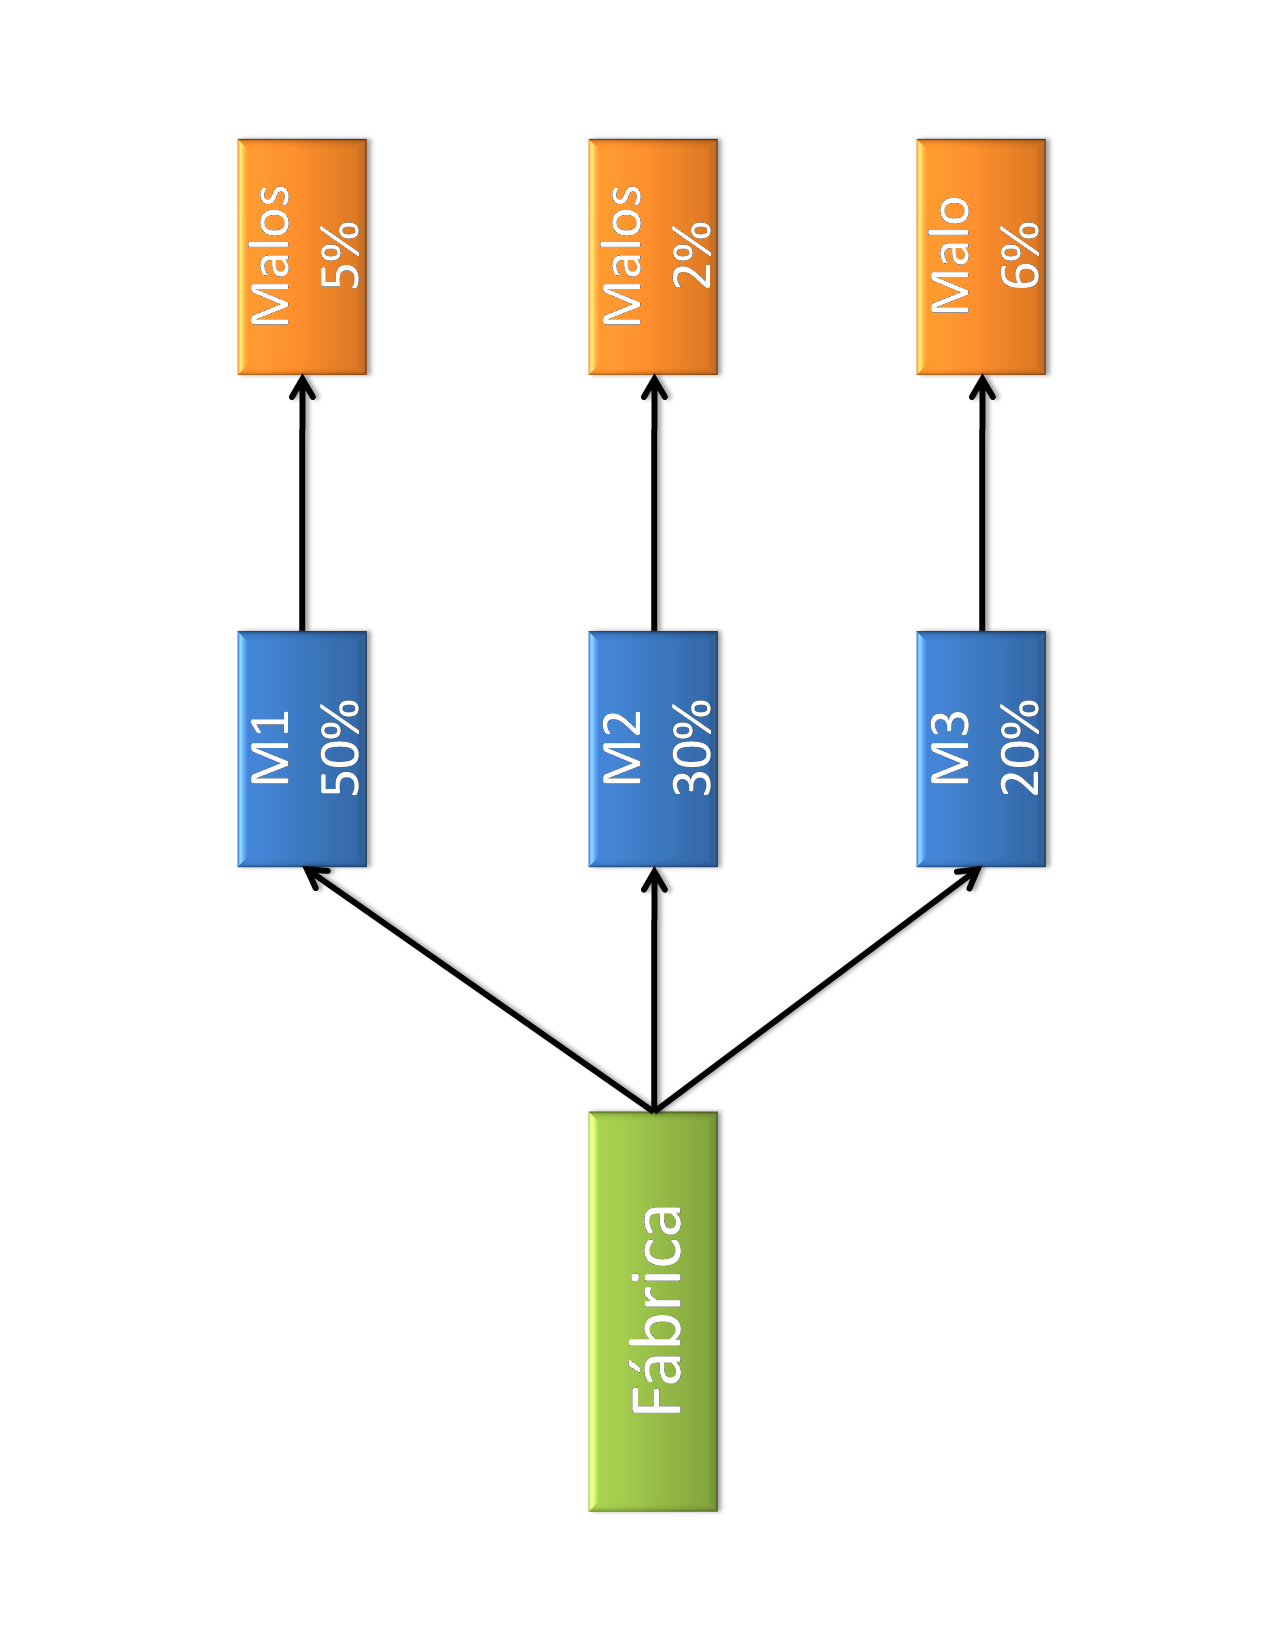
\includegraphics[angle=-90, scale=0.5]{Fabrica1.pdf}
\caption{\emph{Plano del proceso industrial en la fábrica de bolígrafos}}
\end{figure}

Una pregunta natural que surge es acerca de la probabilidad de selección de un artículo defectuoso y para responder a esta pregunta con <<rigurosidad de probabilísta>> es necesario enfocar nuestra atención en los tópicos básicos que dejamos atrás. En primer lugar el experimento en cuestión es la selección de un bolígrafo. Para este experimento, una terna $(\Omega, \mathfrak{F}, P)$ \footnote{$\Omega$ denota el conjunto de todos lo posibles resultados del experimento, $\mathfrak{F}$ denota una $\sigma$-álgebra y $P$ hace referencia ana medida de probabilidad propiamente definida.}, llamada comúnmente espacio de medida o espacio de probabilidad, está dada por
\begin{enumerate}
  \item El espacio muestral: $\Omega=\{\text{defectuoso}, \text{No defectouso}\}$
  \item La $\sigma$-álgebra: $\mathfrak{F}=\{\Omega, \phi, \{\text{Defectuoso}\}, \{\text{No Defectuoso}\}\}$
  \item La función de probabilidad:
  \begin{align*}
  p: \mathfrak{F} &\longrightarrow [0,1]\\
     \Omega &\longrightarrow 1\\
     \phi &\longrightarrow 0\\
     \{Defectuoso\}&\longrightarrow P(D)\\
     \{Defectuoso\}&\longrightarrow 1-P(D)
  \end{align*}
  en donde, acudiendo al teorema de probabilidad total, se define
  \begin{equation*}
  p(D)=p(D \mid M1)P(M1)+p(D \mid M2)P(M2)+p(D \mid M3)P(M3)
  \end{equation*}
\end{enumerate}

Sin embargo, también es posible plantearse otro tipo de preguntas que sirven para calibrar el proceso de producción de artículos defectuosos. Por ejemplo, cabe preguntarse acerca de la probabilidad de que habiendo seleccionado un artículo defectuoso, éste provenga de la primera máquina\footnote{Por supuesto que la pregunta también es válida al indagar por la probabilidad de que habiendo seleccionado un artículo defectuoso, éste provenga de la segunda o tercera máquina.}. En esta ocasión, el experimento ha cambiado y ahora se trata de seleccionar un artículo defectuoso y para responder a tal cuestionamiento, se debe establecer rigurosamente el espacio de probabilidad que puede estar dado por
\begin{enumerate}
  \item El espacio muestral: $\Omega=\{M1, M2, M3 \}$
  \item La $\sigma$-álgebra: $\mathfrak{F}^+=\{\Omega, \phi, \{M1\}, \{M2,M3\}\}$
  \item La función de probabilidad:
  \begin{align*}
  p: \mathfrak{F}^+ &\longrightarrow [0,1]\\
     \Omega &\longrightarrow 1\\
     \phi &\longrightarrow 0\\
     \{M1\}&\longrightarrow p(M1 \mid D)\\
     \{M2,M3\}&\longrightarrow 1-p(M1 \mid D)
  \end{align*}
  en donde, acudiendo a la definición de probabilidad condicional, se define
  \begin{equation*}
  p(M1 \mid D)=\frac{p(D \mid M1)P(M1)}{p(D \mid M1)P(M1)+p(D \mid M2)P(M2)+p(D \mid M3)P(M3)}
  \end{equation*}
\end{enumerate}

La anterior función de probabilidad se conoce con el nombre de regla de probabilidad de Bayes y, aparte de ser el baluarte de la mayoría de investigaciones estadísticas que se plantean hoy en día, ha sido la piedra de tropiezo de muchos investigadores radicales que trataron de estigmatizar este enfoque tildando a sus seguidores de mediocres matemáticos y pobres probabilistas afirmando que la regla de probabilidad de Bayes es sólo un artilugio diseñado para divertirse en el tablero.

Pues bien, la interpretación de la regla de bayes se puede realizar en el sentido de actualización de la estructura probabilística que gobierna el experimento. Y esta actualización tiene mucho sentido práctico cuando se cae en la cuenta de que la vida real está llena de calibradores y que las situaciones generadas son consecuencia de algún cambio estructural. De esta forma, el conocimiento de la probabilidad de que el artículo sea producido por la primera máquina se actualiza al conocer que este artículo particular es defectuoso y de esta manera calibra la estructura aleatoria que existe detrás del contexto de la fábrica de bolígrafos. Aparte de servir para resolver problemas como el anteriormente mencionado, la regla de bayes ha marcado el comienzo de un nuevo enfoque de análisis de datos, no solamente porque hace explícitas las relaciones causales entre los procesos aleatorios, sino también porque facilita la inferencia estadística y la interpretación de los resultados.
\end{Eje}

En el campo de la medicina, también se ha visto un gran número de la aplicación del teorema de Bayes. A continuación se enuncia uno de ellos:

\begin{Eje}
El Grupo de Trabajo de Servicios Preventivos de los Estados Unidos (USPSTF por sus siglas en inglés) hizo unas nuevas y controversiales recomendaciones sobre la detección del cáncer de mama (ver página $http://www.uspreventiveservicestaskforce.org/uspstf/uspsbrca.htm$), dentro de los cuales, no recomienda el examen de la mamografía en mujeres entre 40 y 49 años de edad, afirmando que la práctica bienal de este examen debe ser una decisión individual según el contexto particular de la paciente, mientras que por muchos años, se han dicho a las mujeres que se debe realizar la mamografía una vez cumplidos los 40 años. Por otro lado, USPSTF sí recomienda tal práctica de forma bienal en grupos de mujeres de entre 50 y 74 años de edad, puesto que USPSTF no encontró suficiente evidencia de beneficio o daño adicional en realizar este examen en mujeres mayores que los 74 años. Otra recomendación que hizo USPSTF es no realizar auto exámanes de senos, contrario a las recomendaciones y consejos que da la mayoría de los profesionales y organizaciones de la salud, incluyendo la \emph{Amerian Cancer Society} (ver $http://www.cancer.org/acs/groups/cid/documents/webcontent/003164-pdf.pdf$).

El autor del blog, después de algunas averiguaciones, encontró que 
\begin{itemize}
    \item Los expertos estiman que un 12.3\% de las mujeres desarrollan formas invasivas del cáncer de mama durante la vida.
    \item La probabilidad de que una mujer desarrolle el cáncer de mama entre los 40 y los 49 años de edad es 1 en 69, y esta probabilidad aumenta a medida que envejezca, de tal forma que llega a ser de 1 en 38 en mujeres de entre 50 y 59 años.
    \item El cáncer de mama es más difícil de detectar en mujeres jóvenes puesto que el tejido mamario es más denso y fibroso. Los expertos estiman que la tasa de un falso positivo es de 97.8 por cada 1000 mujeres de 40 y 49 años, y esta tasa disminuye a 86.6 por cada 1000 mujeres entre 50 y 59 años. 
    \item La tasa de un falso negativo es de 1 por cada 1000 mujeres de 40 y 49 años, y es de 1.1 por cada 1000 mujeres entre 50 y 59 años.
\end{itemize}

Resumiendo las anteriores afirmaciones, tenemos las siguientes probabilidades
\begin{table}[!h]
\centering
  \begin{tabular}{|c|c|c|}\hline
  Probabilidad&\multicolumn{2}{|c|}{Edad}\\\cline{2-3}
  &40 - 49 años&50 - 59 años\\\hline
  $p(\text{Cáncer})$&1/69=0.01449&1/38=0.02632\\
  $p(\text{No cáncer})$&68/69=0.9855&37/38=0.97368\\
  $p(\text{Positivo}|\text{ No cáncer})$&0.0978&0.0866\\
  $p(\text{Negativo}|\text{ No cáncer})$&0.9022&0.9134\\
  $p(\text{Negativo}|\text{ Cáncer})$&0.001&0.0011\\
  $p(\text{Positivo}|\text{ Cáncer})$&0.999&0.9989\\\hline
  \end{tabular}
\end{table}

Utilizando la regla de Bayes, se puede calcular las siguientes probabilidades para mujeres de 40 y 49 años: 
\begin{align*}
P(\text{Cáncer}|\text{Positivo})&=\frac{P(\text{Positivo}|\text{Cáncer})P(\text{Cáncer})}{P(\text{Positivo}|\text{Cáncer})P(\text{Cáncer})+P(\text{Positivo}|\text{No cáncer})P(\text{No cáncer})}\\
&=\frac{0.999*0.01449}{0.999*0.01449+0.0978*0.9855}\\
&=0.1305
\end{align*}

\begin{align*}
P(\text{Cáncer}|\text{Negativo})&=\frac{P(\text{Negativo}|\text{Cáncer})P(\text{Cáncer})}{P(\text{Negativo}|\text{Cáncer})P(\text{Cáncer})+P(\text{Negativo}|\text{No cáncer})P(\text{No cáncer})}\\
&=\frac{0.001*0.01449}{0.001*0.01449+0.9022*0.9855}\\
&=0.0000163
\end{align*}

Similarmente, se puede calcular estas dos probabilidades para las mujeres de 50 y 59 años.
\begin{table}[!h]
\centering
  \begin{tabular}{|c|c|c|}\hline
  Probabilidad&\multicolumn{2}{|c|}{Edad}\\\cline{2-3}
  &40 - 49 años&50 - 59 años\\\hline
  $P(\text{Cáncer}|\text{Positivo})$&0.1305985&0.23769\\
  $P(\text{Cáncer}|\text{Negativo})$&0.0000163&0.0000326\\
  $P(\text{No cáncer}|\text{Positivo})$&0.8694223&0.7623123\\
  $P(\text{No cáncer}|\text{Negativo})$&0.9999837&0.9999674\\\hline
  \end{tabular}
\end{table}
Los resultados de la anterior tabla muestran cómo se cambia la probabilidad de tener cancer condicionado en los resultados de la pruebe. Entre estos valores se puede ver que, con un resultado positivo en el examen, la probabilidad de tener efectivamente el cáncer es aproximadamente diez puntos porcentuales más bajo en mujeres de edad de 40 y 49 años, de donde se puede sustentar la recomendación de no efectuar este examen en mujeres de este rango de edad.
\end{Eje}

\section{Inferencia bayesiana}

El enfoque bayesiano, además de especificar un modelo para los datos observados $\mathbf{Y}=(y_1,\ldots,y_n)$ dado un vector de parámetros desconocidos $\btheta=(\theta_1,\ldots,\theta_K)$, usualmente en forma de densidad condicional  $p(\mathbf{Y} \mid \btheta)$, supone que $\btheta$ es aleatorio y que tiene un densidad \emph{previa} $p(\btheta \mid \bEta)$, donde $\bEta$ es un vector de hiper-parámetros. De esta forma, la inferencia concerniente a $\btheta$ se basa en una densidad \emph{posterior} $p(\btheta \mid \mathbf{Y})$.

En términos de estimación, inferencia y predicción, el enfoque Bayesiano supone dos momentos o etapas:

\begin{enumerate}
  \item Antes de la recolección de las datos, en donde el investigador propone, basado en su conocimiento, experiencia o fuentes externas, una distribución de probabilidad \emph{previa} para el parámetro de interés. Con esta distribución es posible calcular estimaciones puntuales y por intervalo con el fin de confirmar que la distribución propuesta se ajusta al problema de estudio. En esta etapa, basados en la distribución \emph{previa}, también es posible hacer predicciones de cantidades observables.
  \item Después de la recolección de los datos. Siguiendo el teorema de Bayes, el investigador actualiza su conocimiento acerca del comportamiento probabilístico del parámetro de interés mediante la distribución \emph{posterior} de este. Con esta distribución es posible calcular estimaciones puntuales y por intervalo justo como en el enfoque frecuentista. En esta etapa, basados en la distribución \emph{posterior}, también es posible hacer predicciones de cantidades observables y pruebas de hipótesis acerca de la adecuación del mejor modelo a los datos observados.
\end{enumerate}

\subsection{Inferencia \emph{previa}}

Con las anteriores expresiones es posible calcular la probabilidad \emph{previa} de que $\btheta$ esté en una determinada región $G$ como
\begin{equation}
Pr(\btheta\in G)=\int_G p(\btheta \mid \bEta)\ d\btheta
\end{equation}

En esta primera etapa también es posible calcular, con fines confirmatorios \cite{Carlin96}, la estimación puntual para el vector $\btheta$ dada por alguna medida de tendencia central para la distribución $p(\btheta \mid \bEta)$. En particular, si se escoge la media, entonces
\begin{equation}\label{est.prio}
\hat{\btheta}=E(\btheta)=\int \btheta \ p(\btheta \mid \bEta)\ d\btheta
\end{equation}

También es posible calcular una región $C$ de $100\times(1-\alpha)\%$ de credibilidad\footnote{La interpretación de las regiones de credibilidad bayesianas difiere de la interpretación de las regiones de confianza frecuentistas. La primera se refiere a la probabilidad de que el verdadero valor de $\btheta$ esté en la región. La segunda se refiere a la región de la distribución muestral para $\btheta$ tal que, dados los datos observados, se podría esperar que el $100\times\alpha\%$ de las futuras estimaciones de $\btheta$ no pertenecieran a dicha región.} para $\btheta$ que en esta primera etapa es tal que
\begin{equation}
1-\alpha \leq Pr(\btheta \in C)=\int_Cp(\btheta \mid \bEta)\ d\btheta
\end{equation}

\subsection{Inferencia \emph{posterior}}
Una vez recolectados los datos, se actualizan las cálculos descritos en la sección anterior. Podemos calcular la probabilidad \emph{posterior} de que $\btheta$ esté en la región $G$ dados los datos observados como
\begin{equation}
Pr(\btheta\in G  \mid \mathbf{Y})=\int_G p(\btheta \mid \mathbf{Y})\ d\btheta
\end{equation}

También es posible calcular la estimación puntual para el vector $\btheta$ dados los datos observados. Ésta está dada por alguna medida de tendencia central para la distribución $p(\btheta \mid \mathbf{Y})$. En particular, si se escoge la media, entonces
\begin{equation}
\hat{\btheta}=E(\btheta \mid \mathbf{Y})=\int \btheta \ p(\btheta \mid \mathbf{Y})\ d\btheta
\end{equation}

La región $C$ de $100\times(1-\alpha)\%$ de credibilidad es tal que
\begin{equation}
1-\alpha \leq Pr(\btheta \in C \mid \mathbf{Y})=\int_Cp(\btheta \mid \mathbf{Y})\ d\btheta
\end{equation}

También la distribución posterior del parámetro $\btheta$ es útil para el procedimiento de juzgamiento de hipótesis en el ámbito del análisis bayesiano. Esto se lleva a cabo por medio del factor de Bayes que se presentará más adelante.

\subsection{Inferencia predictiva}

En términos de inferencia predictiva existen dos etapas que cubren las <<actuales>> suposiciones acerca del vector de parámetros $\btheta$. En una primera etapa - antes de la observación de los datos - la suposición <<actual>> de $\btheta$ está dada por la densidad  \emph{previa} $p(\btheta \mid \bEta)$. En estos términos, utilizando el Resultado \ref{Res131},  la distribución predictiva  \emph{previa} de $\mathbf{Y}$ está dada por
\begin{equation}
p(\mathbf{y})=\int p(\mathbf{Y} \mid \btheta)p(\btheta \mid \bEta)\ d\btheta
\end{equation}

La segunda etapa - después de la recolección de los datos - actualiza las suposiciones acerca de $\btheta$ puesto que ahora éste sigue una distribución \emph{posterior} dada por (\ref{Bayes}). Por lo tanto, la distribución predictiva  \emph{posterior} de $\mathbf{Y}$ está dada por
\begin{align}\label{predictpos}
p(\tilde{\mathbf{y}} \mid \mathbf{Y})&=\int p(\tilde{\mathbf{y}},\btheta \mid \mathbf{y})\ d\btheta \notag \\
&=\int p(\tilde{\mathbf{y}} \mid \btheta,\mathbf{Y})p(\btheta \mid \mathbf{Y})\ d\btheta \notag \\
&=\int p(\tilde{\mathbf{y}} \mid \btheta)p(\btheta \mid \mathbf{Y})\ d\btheta
\end{align}
donde $p(\tilde{\mathbf{y}} \mid \btheta)$ es la distribución de los datos evaluada en los nuevos valores $\tilde{\mathbf{y}}$. La segunda línea de la anterior igualdad se obtiene utilizando el resultado \ref{Res121}  y la última línea se obtiene del resultado \ref{Res122} de la independencia condicional.

\section{Información \emph{previa}}

La escogencia de una distribución previa es muy importante en el análisis bayesiano, puesto que ésta afecta directamente en la distribución posterior, tal como lo ilustra el teorema de Bayes. En primer lugar, la distribución previa debe describir adecuadamente los conocimientos previos sobre los parámetros objetivos de estimación. Por ejemplo, si se cree que un parámetro toma valores cercanos a 10, entonces la distribución escogida para representarla también debe tomar valores cercanos a 10, por ejemplo, una distribución normal centrada en ese valor. Por otro lado, dado que en la literatura existe un gran número de distribuciones, algunas muy similares entre ellas, a la hora de escoger una distribución previa también debe tener en cuenta las implicaciones a la hora de efectuar cálculos de la estimación puntual o de intervalo de crediblidad, procurando en la mayoría de casos, obtener una distribución posterior fácil de manejar. A continuación exponemos algunos aspectos generales relacionados con esta distribución previa.

\subsection{Distribuciones conjugadas}

Como se verá en los capítulos siguientes, muchos problemas de inferencia bayesiana comparten la agradable cualidad de que la forma funcional de la distribución \emph{previa} para el parámetro de interés resulta ser la misma de la distribución \emph{posterior}. Por ejemplo:

\begin{itemize}
  \item Cuando se tiene una muestra aleatoria de variables con distribución Bernoulli de parámetro $\theta$, es factible pensar que una distribución \emph{previa} apropiada para este parámetro es la distribución Beta; bajo este escenario, la distribución \emph{posterior} también resulta ser Beta.
  \item En el caso en que se quiera modelar el parámetro $\theta$ concerniente a una variable aleatoria con distribución Poisson, es posible asignar como candidata para distribución \emph{previa} a la distribución Gamma; en este caso la distribución \emph{posterior} también resulta ser Gamma.
\end{itemize}

Las distribuciones conjugadas son deseadas en el análisis bayesiano pues en primer lugar, la distribución posterior del parámetro $\theta$ es considerada como la actualización del conocimiento acerca de este después de la recolección de los datos, entonces al tener la misma forma funcional que la distribución previa, puede ser comparada a ésta y así ver claramente cómo es la influencia de los datos observados sobre la creencia acerca de $\theta$; en segundo lugar, el hecho de que la distribución posterior sea de la misma forma funcional que la previa permite que la actualización de información se pueda llevar a cabo sistemáticamente, pues cada vez que se observan nuevos datos, la anterior distribución posterior puede ser tomada como la distribución previa y así producir una nueva distribución posterior. 

A continuación exponemos la definición rigurosa de las distribuciones conjungadas y algunos tópicos relacionados.

\begin{Defi}
Sea $\mathcal{F}=\{p(\mathbf{Y} \mid \btheta)\}$ una familia de distribuciones de probabilidad. Una familia de distribuciones $\mathcal{P}$ se dice conjugada con respecto a $\mathcal{F}$ si para toda distribución \emph{previa} $p(\btheta) \in \mathcal{P}$ y para toda distribución de muestreo o verosimilitud de las observaciones $p(\mathbf{Y} \mid \btheta)$, $p(\btheta \mid \mathbf{Y})$ también pertenece a la familia $\mathcal{P}$.
\end{Defi}

Esta definición es en la mayoría de los casos prácticos muy útil. Sin embargo, \citeasnoun{Migon} describe los siguientes dos casos en donde esta definición es completamente inútil:

\begin{enumerate}
\item (Caso amplio) Sea $\mathcal{P}=\{\emph{Todas las distribuciones de probabilidad}\}$ y $\mathcal{F}$ cualquier familia de distribuciones de probabilidad. Entonces $\mathcal{P}$ es conjugada con respecto a $\mathcal{F}$ puesto que toda posible distribución \emph{posterior} será un miembro de $\mathcal{P}$.
\item (Caso restringido) Sea $\mathcal{P}=\{p  \mid  p(\theta=\theta_0)=1\}$, esto es, $\mathcal{P}$ corresponde a todas las distribuciones concentradas en un punto. Sea $\mathcal{F}$ cualquier familia de distribuciones de probabilidad. De esta manera, la distribución \emph{posterior} de $\theta$ estará dada por
    \begin{align*}
    p(\theta \mid Y)\propto
    p(Y \mid \theta)p(\theta)
    &=
    \begin{cases}
    p(Y \mid \theta)\times 1 \ \ \ \ \text{si $\theta=\theta_0$}\\
    p(Y \mid \theta)\times 0 \ \ \ \ \text{si $\theta\neq\theta_0$}\\
    \end{cases}\\
    &=
    \begin{cases}
    p(Y \mid \theta) \ \ \ \ \text{si $\theta=\theta_0$}\\
    0           \ \ \ \ \text{si $\theta\neq\theta_0$}\\
    \end{cases}
    \end{align*}

    De lo anterior y dado que $\int p(\theta \mid Y)\ d\theta=1$, entonces $p(Y \mid \theta)=1$ si y sólo si $\theta=\theta_0$. Con el anterior razonamiento, se concluye que $\mathcal{P}$ es conjugada con respecto a $\mathcal{F}$.
\end{enumerate}

Por lo tanto, se deben buscar distribuciones \emph{previa} que sean conjugadas de una forma tan amplia que permita proponer una distribución \emph{previa} adecuada, pero al mismo tiempo tan restringida para que la definición de conjugada tenga sentido práctico. Ahora introducimos una familia de distribuciones muy importante para el desarrollo de la teoría estadística, tanto en el ámbito bayesiano como en el clásico.

\subsubsection*{Familia exponencial}

Dependiendo de la naturaleza del parámetro $\theta$, la familia exponencial puede ser uniparamétrica o multiparamétrica. En el primer caso, una distribución de probabilidad pertenece a la familia exponencial uniparamétrica si se puede escribir de la forma
\begin{equation}\label{uniexpo}
p(Y \mid \theta)=\exp\{d(\theta)T(y)-c(\theta)\}h(y)
\end{equation}

donde $T(y)$ y $h(y)$ son funciones que dependen de $y$ únicamente, y $d(\theta)$ y $c(\theta)$ son funciones que depende de $\theta$ únicamente. Análogamente, una distribución de probabilidad pertenece a la familia exponencial multi-paramétrica si se puede escribir de la forma
\begin{equation}\label{multiexpo}
p(Y \mid \btheta)=\exp\{\mathbf{d}(\btheta)'\mathbf{T}(y)-c(\btheta)\}h(y)
\end{equation}
donde $\mathbf{T}(y)$ y $\mathbf{d}(\btheta)$ son funciones vectoriales, $h(y)$ y $c(\btheta)$ son funciones reales.

La ventaja de la familia exponencial radica en que es una familia relativamente restringuida de distribuciones y a la vez conserva la propiedad de ser distribuciones conjugadas, tal como muestra el siguiente resultado:

\begin{Res}\label{FE1}
Sea $Y$ una variable aleatoria con función de densidad perteneciente a la familia exponencial uniparamétrica, entonces la familia exponencial uniparamétrica es conjugada con respecto a sí misma.
\end{Res}

\begin{proof}
Observando la expresión (1.5.1), se debe encontrar una distribución \emph{previa} en la familia exponencial uniparamétrica, tal que la distribución \emph{posterior}, resultante del producto de la distribución \emph{previa} con la verosimilitud, sea también miembro de la familia exponencial uniparamétrica. Con base en lo anterior, la distribución \emph{previa}, parametrizada por el hiperparámetro $\alpha$, debe ser una función exponencial de los términos $d(\theta)$ y $c(\theta)$ como lo afirma \citeasnoun{Jordan}. Esto es,
\begin{equation}
p(\theta \mid \alpha)\propto\exp\{w(\alpha) d(\theta)-\delta c(\theta)\},
\end{equation}

donde $\delta$ es una constante real (posiblemente dependiente de $\alpha$). Por otro lado, para garantizar que $p(\theta \mid \alpha)$ sea una auténtica función de densidad se normaliza de la siguiente manera
\begin{equation}
p(\theta \mid \alpha)=\frac{1}{k(\alpha,\delta)}\exp\{w(\alpha) d(\theta)-\delta c(\theta)\},
\end{equation}

con
\begin{equation*}
k(\alpha,\delta)=\int\exp\{w(\alpha) d(\theta)-\delta c(\theta)\} \ d\theta.
\end{equation*}

De esta manera, no es difícil comprobar que la definición de distribución \emph{previa}, parametrizada por el hiper-parámetro $\alpha$, pertenece a la familia exponencial, puesto que
\begin{equation}
p(\theta \mid \alpha)=\exp\{\underbrace{w(\alpha)}_{d(\alpha)} \underbrace{d(\theta)}_{T(\theta)} - \underbrace{\ln k(\alpha,\delta)}_{c(\alpha)}\}\underbrace{\exp\{-\delta c(\theta)\}}_{h(\theta)}.
\end{equation}

Por otro lado, del teorema de Bayes se tiene que
\begin{align*}
p(\theta \mid Y) &\propto p(Y \mid \theta)p(\theta \mid \alpha)\\
&=\exp\{w(\alpha) d(\theta) + d(\theta)T(y) - c(\theta) -\ln k(\alpha,\delta) \}\exp\{-\delta c(\theta)\}h(y)\\
&=\exp\{\underbrace{[\alpha+T(y)]}_{d(y)} \underbrace{d(\theta)}_{T(\theta)} -\underbrace{[\ln k(\alpha,\delta)-\ln h(y)]}_{c(y)}\} \underbrace{\exp\{-(\delta+1) c(\theta)\}}_{h(\theta)}\\
&\propto \exp\{[w(\alpha)+T(y)] d(\theta)\}\exp\{-(\delta+1) c(\theta)\}.
\end{align*}

Por lo tanto, la distribución \emph{posterior} resultante también pertenece a la familia exponencial uniparamétrica.
\end{proof}

La extensión del anterior resultado para el caso cuando tenemos una muestra aleatoria de observaciones es sencilla, tal como se expone a continuación:
\begin{Res}
Sean $\mathbf{Y}=\{Y_1, \ldots, Y_n\}$ una muestra aleatoria de variables distribuidas con función de densidad común perteneciente a la familia exponencial uniparamétrica, cuya función de densidad conjunta $p(\mathbf{Y} \mid \theta)$ también pertenece a la familia exponencial uniparamétrica. Bajo las anteriores condiciones la familia exponencial uniparamétrica es conjugada con respecto a sí misma.
\end{Res}

\begin{proof}
La demostración es inmediata utilizando el resultado anterior y notando que la forma funcional de la densidad conjunta para $\mathbf{Y}$ es
\begin{equation}
p(\mathbf{Y} \mid \theta)=\exp\left\{d(\theta)\sum_{i=1}^nT(y_i)-nc(\theta)\right\}\prod_{i=1}^nh(y_i)
\end{equation}
la cual hace parte de la familia exponencial.
\end{proof}

Otra extensión del resultado \ref{FE1} corresponde al caso cuando la distribución de la observación está reparametrizado por un vector de parámetros $\btheta$. A continuación se expone el resultado y la prueba correspondiente.

\begin{Res}
Sean $Y$ una variable aleatoria con función de densidad perteneciente a la familia exponencial multiparamétrica. Sea $\btheta$ el parámetro de interés con distribución \emph{previa} parametrizada por un vector de hiperparámetros $\bEta$ y perteneciente a la familia exponencial multiparamétrica. Entonces la familia exponencial multiparamétrica es conjugada con respecto a sí misma.
\end{Res}

\begin{proof}
En primer lugar, la distribución de probabilidad de $Y$ perteneciente a la familia exponencial  multiparamétrica está dada por (1.5.2). Siguiendo el mismo razonamiento de la demostración del Resultado 1.5.1, la distribución \emph{previa} del parámetro de interés debe estar definida de la siguiente manera
\begin{equation}
p(\btheta \mid \bEta)=\exp\left\{\underbrace{w(\bEta)'}_{\mathbf{d}(\bEta)}
\underbrace{\mathbf{d}(\btheta)}_{\mathbf{T}(\btheta)} - \underbrace{\ln k(\bEta,\delta)}_{c(\bEta)}\right\}\underbrace{\exp\{-\delta c(\btheta)\}}_{h(\btheta)},
\end{equation}

con
\begin{equation*}
k(\bEta,\delta)=\int\exp\{w(\bEta)'\mathbf{d}(\btheta)-\delta c(\btheta)\} \ d\btheta.
\end{equation*}

Utilizando el teorema de Bayes, se tiene que, la distribución \emph{posterior} del parámetro $\theta$ es
\begin{align*}
p(\btheta \mid Y) &\propto p(Y \mid \btheta)p(\btheta \mid \bEta)\\
&= \exp\{\mathbf{T}(y)'\mathbf{d}(\btheta) - c(\btheta) + w(\bEta)' \mathbf{d}(\btheta) - \delta c(\btheta) - \ln k(\bEta,\delta) +\ln h(y)\}\\
& =
\exp\left\{\underbrace{(w(\bEta)+\mathbf{T}(y))'}_{\mathbf{d}(y)}
\underbrace{\mathbf{d}(\btheta)}_{\mathbf{T}(\theta)} - \underbrace{\left[\ln k(\bEta,\delta)-\ln h(y)\right]}_{c(y)}\right\}\underbrace{\exp\{-(\delta+1)c(\btheta)\}}_{h(\btheta)}
\end{align*}

La anterior expresión también hace parte de la familia exponencial biparamétrica y con esto se concluye la demostración
\end{proof}

Nótese que el anterior resultado también cobija situaciones donde la verosimilitud sea perteneciente a la familia exponencial uniparamétrica. Más aún, a cualquier familia exponencial multiparamétrica de orden menor o igual al orden de la distribución \emph{previa}.

\begin{Res}
Sean $\mathbf{Y}=\{Y_1, \ldots, Y_n\}$ una muestra aleatoria con función de densidad conjunta o verosimilitud dada (1.4.4). Bajo este escenario la familia exponencial multi-paramétrica es conjugada con respecto a sí misma.
\end{Res}

\begin{proof}
La demostración sigue los mismos lineamentos que la demostración del resultado anterior concluyendo que la distribución \emph{posterior} de $\btheta$ está dada por
\begin{align*}
&p(\btheta \mid \mathbf{Y}) \propto p(\mathbf{Y} \mid \btheta)p(\btheta \mid \bEta)\\
&= \exp\left\{\sum_{i=1}^n\mathbf{T}(y_i)'\mathbf{d}(\btheta) - nc(\btheta) + \bEta' \mathbf{d}(\btheta) - \delta c(\btheta) - \ln k(\bEta,\delta) +\sum_{i=1}^n\ln h(y_i)\right\}\\
& =\exp\left\{\underbrace{\left(\bEta+\sum_{i=1}^n\mathbf{T}(y_i)\right)'}_{\mathbf{d}(\mathbf{y})}
\underbrace{\mathbf{d}(\btheta)}_{\mathbf{T}(\theta)} - \underbrace{\left[\ln k(\bEta,\delta)-\sum_{i=1}^n\ln h(y_i)\right]}_{c(\mathbf{y})}\right\} \\
&  \times \underbrace{\exp\left\{-(\delta+n)c(\btheta)\right\}}_{h(\btheta)}
\end{align*}
La anterior expresión también hace parte de la familia exponencial.
\end{proof}

Ahora, estudiamos las expresiones relacionadas con la distribución predictiva de nuevas observaciones dentro del contexto de la familia exponencial:
\begin{Res}
Sea $Y$ una variable aleatoria con función de densidad perteneciente a la familia exponencial, dada por (\ref{uniexpo}). Sea $\theta$ el parámetro de interés con distribución \emph{previa} en la familia exponencial biparamétrica. La distribución predictiva \emph{previa} de $Y$ está dada por
\begin{equation}
p(Y)=\frac{k(\alpha+T(y),\delta+1)}{k(\alpha,\delta)}h(y)
\end{equation}

donde 
\begin{equation*}
k(a,b)=\int \exp\{w(a) d(\theta)-b c(\theta)\}\ d\theta
\end{equation*}
\end{Res}

\begin{proof}
\begin{align*}
p(Y)&=\int p(\theta)p(Y \mid \theta)\ d\theta\\
&=\int \exp\{w(\alpha) d(\theta)-\ln k(\alpha,\delta)-\delta c(\theta)\}\exp\{d(\theta)T(y)-c(\theta)\}h(y)d\theta\\
&=\frac{h(y)}{k(\alpha,\delta)}\int \exp\{[w(\alpha)+T(y)]d(\theta)-(\delta+1)c(\theta)\}d\theta\\
&=\frac{k(\alpha+T(y),\delta+1)h(y)}{k(\alpha,\delta)}
\end{align*}

donde
\begin{equation*}
k(\alpha,\delta)=\int \exp\{w(\alpha) d(\theta)-\delta c(\theta)\}\ d\theta
\end{equation*}

y
\begin{equation*}
k(\alpha+T(y),\delta+1)=\int \exp\{[w(\alpha)+T(y)]d(\theta)-(\delta+1)c(\theta)\} \ d\theta.
\end{equation*}
\end{proof}

La extensión al caso de contar con una muestra aleatoria de observaciones se encuentra a continuación:

\begin{Res}
Sea $\mathbf{Y}=\{Y_1\ldots,Y_n\}$ una muestra aleatoria con función de densidad conjunta perteneciente a la familia exponencial, dada por (1.4.4). Sea $\theta$ el parámetro de interés con distribución \emph{previa} dada por (1.4.5). La distribución predictiva \emph{previa} de $\mathbf{Y}$ está dada por

\begin{equation}
p(\mathbf{Y})=\frac{k(\alpha+T(\mathbf{y}),\delta+n)}{k(\alpha,\beta)}h(\mathbf{y})
\end{equation}
donde $k$ se define tal como en el resultado anterior.
\end{Res}

\begin{proof}
La prueba se tiene de inmediato siguiendo los lineamentos de la demostración del anterior resultado.
\end{proof}

\begin{Res}
En términos de la distribución predictiva \emph{posterior}, se tiene que para una sola observación $\tilde{y}$, ésta está dada por
\begin{equation}
p(\tilde{y} \mid Y)=\frac{k(\alpha+T(y)+T(\tilde{y}),\delta+2)}{k(\alpha+T(y),\delta+1)}h(\tilde{y})
\end{equation}
y en el caso en donde se tiene una muestra aleatoria, entonces la distribución predictiva \emph{posterior} para una nueva muestra $\tilde{\mathbf{y}}=\{\tilde{y}_1,\ldots,\tilde{y}_{n^*}\}$ de tamaño $n^*$ está dada por
\begin{equation}
p(\tilde{\mathbf{y}} \mid \mathbf{Y})=
\frac{k(\alpha+T(\mathbf{y})+T(\tilde{\mathbf{y}}),\delta+n+n^*)}
{k(\alpha+T(\mathbf{y}),\delta+n)}h(\tilde{\mathbf{y}})
\end{equation}
\end{Res}

\begin{proof}
De la definición de distribución predictiva \emph{posterior} dada por la expresión (\ref{predictpos}) se tiene que
\begin{align*}
p(\tilde{y} \mid Y)&=\int p(\tilde{y} \mid \theta)p(\theta \mid y)\ d\theta\\
&=\int \exp\{d(\theta)T(\tilde{y})-c(\theta)\}h(\tilde{y})\dfrac{\exp\{[w(\alpha)+T(y)]d(\theta)-(\delta+1)c(\theta)\}}{k(\alpha+T(y),\delta+1)}\ d\theta\\
&=\frac{h(\tilde{y})}{k(w(\alpha)+T(y),\delta+1)}\int \exp\{[\alpha+T(y)+T(\tilde{y})]d(\theta)-(\delta+2)c(\theta)\}\ d\theta\\
&=\frac{k(\alpha+T(y)+T(\tilde{y}),\delta+2)}{k(\alpha+T(y),\delta+1)}h(\tilde{y}),
\end{align*}

con
\begin{equation*}
k(\alpha+T(y)+T(\tilde{y}),\delta+2)=\int \exp\{[w(\alpha)+T(y)+T(\tilde{y})]d(\theta)-(\delta+2)c(\theta)\}\ d\theta.
\end{equation*}

La demostración para la nueva muestra se lleva a cabo de manera análoga.
\end{proof}

\subsection{Distribuciones \emph{previa} no informativas}

Cuando no existe una base poblacional sobre el parámetro de interés o cuando existe total ignorancia de parte del investigador acerca del comportamiento de probabilístico del parámetro, es necesario definir distribuciones \emph{previa} que sean no informativas. Es decir, definir distribuciones \emph{previa} que jueguen un papel mínimo en términos de influencia en la distribución \emph{posterior}. Una característica de estas distribuciones es que su forma es vaga, plana o difusa, cumpliendo así el objetivo de no influenciar a la distribución \emph{posterior}. Por tanto la pregunta de interés que surge en este instante es: ¿cómo seleccionar distribuciones \emph{previa} no informativas\footnote{Existen muchas denominaciones para las distribuciones uniformes que no son informativas. Por ejemplo, Box Tiao proponen el nombre de distribuciones localmente uniformes para asegurar que cumplan con las condiciones de función de densidad de probabilidad en un rango particular del espacio paramétrico. Sin embargo, en este texto vamos a utilizar la expresión <<no informativa>> al referirse a este tipo de distribuciones a previa.} sobre el parámetro de interés?

En los anteriores términos, la distribución uniforme define una distribución \emph{previa} que cumple con las características de no información en la mayoría de escenarios. Específicamente en aquellos problemas en donde el parámetro de interés está limitado a un espacio de muestreo acotado. Por ejemplo, en la distribución Binomial, el parámetro de interés está limitado al espacio de muestreo $[0,1]$. Sin embargo, no en todos los problemas encaja la distribución uniforme. Nótese, por ejemplo, que en el caso en que la distribución exponencial se acomode a los datos como candidata a verosimilitud, entonces el espacio de muestreo del parámetro de interés estaría dado por $(0,\infty)$ en cuyo caso la distribución uniforme no sería conveniente puesto que sería una distribución impropia en el espacio de muestreo del parámetro de interés. Es decir
\begin{equation*}
\text{si } p(\theta)\propto kI_{\Theta}(\theta) \text{, entonces } \int_{\Theta}p(\theta) \ d(\theta)\longrightarrow \infty.
\end{equation*}

donde $\Theta$ denota espacio de muestreo del parámetro $\theta$ y $I$ denota la función indicadora. Por otro lado, una característica importante que debe tener una distribución \emph{previa} no informativa es que sea invariante en términos de transformaciones matemáticas. Es decir, si el parámetro de interés es $\theta$ con distribución \emph{previa} no informativa dada por $p(\theta)$, y sea $\phi=h(\theta)$ una transformaición de $\theta$ por medio de la función $h$, entonces la distribución \emph{previa} de $\phi$ también debería ser no informativa. Sin embargo, la teoría de probabilidad afirma que la distribución de probabilidad de una transformación está dada por
\begin{equation}\label{teo_transf}
p(\phi)=p(\theta) \mid \frac{d\theta}{d\phi} \mid =p(\theta) \mid h'(\theta) \mid ^{-1}
\end{equation}

y claramente si la función $h$ no es una función lineal, entonces los resultados encontrados por medio de este enfoque indicarían que la distribución \emph{previa} $p(\phi)$ sería informativa contradiciendo los supuestos de $p(\theta)$. El siguiente ejemplo ilustra este planteamiento:

\begin{Eje}
Suponga que el parámetro de interés es $\theta$ y que está restringido a un espacio de muestreo dado por el intervalo $[0,1]$. Si se supone completa ignorancia acerca del comportamiento del parámetro, entonces una buena opción, con respecto a la distribución \emph{previa}, sería la distribución uniforme en el intervalo $[0,1]$. Es decir, la distribución \emph{previa} no informativa estaría dada por
\begin{equation*}
p(\theta) = I_{[0,1]}(\theta)
\end{equation*}

Suponga ahora que existe una transformación del parámetro de interés dada por $\phi=h(\theta)=\ln(\theta)$. Por tanto, siguiendo (\ref{teo_transf}) se tiene que la distribución de $\phi$ está dada por
\begin{equation*}
p(\phi)=I_{(-\infty,0)}(\phi)e^{\phi}
\end{equation*}

la cual es informativa con respecto al parámetro $\phi$. Sin embargo, es el mismo problema y existe una contradicción en términos de que para $\theta$ se desconoce todo, pero para una función $\phi$ existe evidencia de que el parámetro se comporta de cierta manera.
\end{Eje}

Para palear las anteriores diferencias, es necesario encontrar una distribución \emph{previa} no informativa que sea invariante a transformaciones matemáticas. La distribución \emph{previa} no informativa de Jeffreys, definida a continuación, cuenta con esta agradable propiedad.

\begin{Defi}
Si la verosimilitud de los datos está determinada por un único parámetro $\theta$, la distribución \emph{previa} no informativa de Jeffreys tiene distribución de probabilidad dada por
\begin{equation}
p(\theta)\propto (I(\theta))^{1/2}
\end{equation}

con $I(\theta)$ la información de Fisher definida como
\begin{align*}
I(\theta)&=E\left\{\left[\frac{\partial}{\partial\theta}\log{p(\mathbf{Y}\mid\theta)}\right]^2\right\}\\
&=-E\left\{\dfrac{\partial^2}{\partial\theta^2}\log{p(\mathbf{Y}\mid\theta)}\right\}
\end{align*}

Si la verosimilitud de los datos está determinada por un vector de parámetros $\btheta$, la distribución \emph{previa} no informativa de Jeffreys tiene distribución de probabilidad dada por
\begin{equation}
p(\theta)\propto |\mathbf{I}(\btheta)|^{1/2}
\end{equation}

donde $\mathbf{I}$ es la matriz de información de Fisher, cuyo elemento en la fila $i$ y columna $j$ está definida como
\begin{align*}
\mathbf{I}_{[ij]}(\btheta)&=E\left\{\left[\frac{\partial}{\partial\theta_i}\log{p(\mathbf{Y}\mid\theta)}\right]\left[\frac{\partial}{\partial\theta_j}\log{p(\mathbf{Y}\mid\btheta)}\right]\right\}\\
&=-E\left\{\dfrac{\partial^2}{\partial\theta_i\partial\theta_j}\log{p(\mathbf{Y}\mid\btheta)}\right\}
\end{align*}
donde $\theta_i$ y $\theta_j$ son los elementos $i$ y $j$ del vector $\btheta$.
\end{Defi}

Nótese que si la verosimilitud de las observaciones pertenecen a la familia de distribuciones exponencial, entonces la distribución previa de Jeffreys no es difícil de calcular. Por otro lado nótese que la distribución previa no informativa de Jeffreys depende, de cierta manera, del mecanismo probabilístico que rige a los datos. Lo anterior hace que ciertos críticos de la estadística bayesiana critiquen este enfoque puesto que se supone que la formulación de la distribución a previa es independiente de los datos observados.

A continuación se evidencia la propiedad de esta distribución previa de seguir siendo no informativa con diferentes parametrizaciones. 
\begin{Res}
La distribución \emph{previa} no informativa de Jeffreys es invariante a transformaciones uno a uno. Es decir, si $\phi=h(\theta)$, entonces $p(\phi)\propto(I(\phi))^{1/2}$.
\end{Res}

\begin{proof}
En primer lugar nótese que
\begin{align*}
I(\theta)=\mathbf{J}(\phi) \mid \frac{\partial\phi}{\partial\theta} \mid ^{2}
\end{align*}

puesto que al utilizar la regla de la cadena del cálculo matemático se tiene que
\begin{align*}
\mathbf{J}(\phi)= - E\left[\frac{\partial^2 \log p(\mathbf{Y} \mid \phi)}{\partial\phi^2}\right]
&= - E\left[\frac{\partial}{\partial\phi}\left(\frac{\partial \log p(\mathbf{Y} \mid \phi)}{\partial\phi}\right)\right]\\
&= - E\left[\frac{\partial}{\partial\theta}\left(\frac{\partial \log p(\mathbf{Y} \mid \phi)}{\partial\phi}\right) \mid \frac{\partial\theta}{\partial\phi} \mid \right]\\
&= - E\left[\frac{\partial^2 \log p(\mathbf{Y} \mid \phi)}{d\theta^2} \mid \frac{\partial\theta}{\partial\phi} \mid ^{2}\right]\\
&= - E\left[\frac{\partial^2 \log p(\mathbf{Y} \mid \theta =h^{-1}(\phi))}{d\theta^2} \mid \frac{\partial\theta}{\partial\phi} \mid ^{2}\right]\\
&= I(\theta) \mid \frac{\partial\theta}{\partial\phi} \mid ^{2}
\end{align*}

Ahora, de la definición de función de distribución para una función y utilizando (1.4.11), se tiene que
\begin{align*}
p(\phi)&=p(\theta) \mid \frac{\partial\theta}{\partial\phi} \mid
\propto (I(\theta))^{1/2} \mid \frac{\partial\theta}{\partial\phi} \mid
\propto I(\phi)^{1/2} \mid \frac{\partial\phi}{\partial\theta} \mid  \mid \frac{d\theta}{\partial\phi} \mid =I(\phi)^{1/2}
\end{align*}
\end{proof}

En \citeasnoun[p. 59]{BoxTiao} citan una Tabla de resumen en donde se encuentran distribuciones a previa no informativas para las distribuciones probabilísticas más comunes. A continuación se exponen algunos ejemplos que utilizan este enfoque.

\begin{Eje}
Si $Y$ es una variable aleatoria con distribución Binomial, entonces el espacio de muestreo del parámetro de interés será el intervalo $[0,1]$; sería conveniente utilizar la función de distribución uniforme sobre este intervalo como distribución \emph{previa} no informativa. Con el enfoque de Jeffreys se llega a este mismo resultado puesto que: la información de Fisher para la distribución binomial es $J(\theta)=n/\theta(1- \theta)$ dado que
\begin{equation*}
\log p(Y \mid \theta)=\log \binom{n}{y} + y\log(\theta)+(n-y)\log(1-\theta)
\end{equation*}
y
\begin{equation*}
\frac{\partial^2 \log p(Y \mid \theta)}{\partial\theta^2}=-\frac{y}{\theta^2}-\frac{n-y}{(1-\theta)^2}
\end{equation*}
Por lo tanto al calcular la esperanza, y por consiguiente la información de Fisher, se tiene que
\begin{equation*}
I(\theta)=- E\left[\frac{d^2 \log p(Y \mid \theta)}{d\theta^2}\right]
=\frac{n\theta}{\theta^2}+\frac{n-n\theta}{(1-\theta)^2}= \frac{n}{\theta(1-\theta)}
\end{equation*}
Es decir, la distribución \emph{previa} no informativa para el parámetro de interés $\theta$ es proporcional a $\theta^{-1/2}(1-\theta)^{-1/2}$, la cual comparte la misma forma estructural de una distribución $Beta(1/2,1/2)$ que a su vez es idéntica a la distribución uniforme.  En términos de la distribución \emph{posterior} para el parámetro de interés, se tiene que
\begin{align*}
p(\theta \mid Y) &\propto p(Y \mid \theta) p(\theta)\\
&\propto \theta^{y}(1-\theta)^{n-y}\theta^{-1/2}(1-\theta)^{-1/2}\\
&=\theta^{y+1/2-1}(1-\theta)^{n-y+1/2-1}
\end{align*}
Por tanto, la distribución de $\theta \mid Y$ es $Beta(y+1/2,n-y+1/2)$. Por construcción, esta distribución no está alterada ni influenciada por la distribución \emph{previa} pues la misma es no informativa.
\end{Eje}

\begin{Eje}
\label{EjemPoisson}
Si $\mathbf{Y}=\{Y_1,\ldots,Y_n\}$ es una muestra aleatoria de variables con distribución de Poisson, entonces el espacio de muestreo del parámetro de interés será el intervalo $(0,\infty)$; por tanto utilizar la distribución uniforme como distribución \emph{previa} no informativa no es conveniente. Ahora, la información de Fisher para la distribución conjunta es $I(\theta)=n/\theta$ puesto que
\begin{equation*}
\log p(\mathbf{Y} \mid \theta)=-n\theta+\log(\theta)\sum_{i=1}^ny_i-\sum_{i=1}^n\log(y_i!)
\end{equation*}
y
\begin{equation*}
\frac{\partial^2 \log p(\mathbf{Y} \mid \theta)}{\partial\theta^2}=-\frac{\sum_{i=1}^ny_i}{\theta^2}
\end{equation*}
Por lo tanto al calcular la esperanza, y por consiguiente la información de Fisher, se tiene que
\begin{equation*}
I(\theta)=- E\left[\frac{\partial^2 \log p(\mathbf{Y} \mid \theta)}{\partial\theta^2}\right]
=\frac{\sum_{i=1}^nE(y_i)}{\theta^2}=\frac{n}{\theta}
\end{equation*}
Es decir, la distribución \emph{previa} no informativa para el parámetro de interés es proporcional a $\theta^{-1/2}$. En términos de la distribución \emph{posterior} para el parámetro de interés, se tiene que
\begin{align*}
p(\theta \mid Y) \propto p(Y \mid \theta) p(\theta) \propto e^{-n\theta} \theta^{\sum_{i=1}^ny_i}\theta^{-1/2}
=e^{-n\theta} \theta^{\sum_{i=1}^ny_i-1/2}
\end{align*}
Por tanto, la distribución de $\theta \mid \mathbf{Y}$ es $Gamma(\sum_{i=1}^ny_i+1/2,n)$. Por construcción, esta distribución no está alterada ni influenciada por la distribución \emph{previa} pues la misma es no informativa.
\end{Eje}

\begin{Eje}
Suponga que $\mathbf{Y}=\{Y_1\ldots, Y_n\}$ es una muestra aleatoria con distribución normal de parámetros $(\theta, \sigma^2)'$. Se puede verificar que la matriz de información de Fisher para el vector de parámetros está dada por
\begin{equation}
\begin{pmatrix}
  \frac{n}{\sigma^2} & 0 \\
  0 & \frac{n}{2\sigma^4} \\
\end{pmatrix}
\end{equation}

cuyo determinante está dado por $\frac{n^2}{2\sigma^6}$. Por lo tanto, la distribución a previa no informativa de Jeffreys está dada por
\begin{equation}
p(\theta,\sigma^2)\propto 1/\sigma^3
\end{equation}
\end{Eje}

\section{Pruebas de hipótesis}

A excepción del juzgamiento de hipótesis, las inferencias que hacen los estadísticos bayesianos, acerca de poblaciones normales, son muy similares a las que los estadísticos de la tradición frecuentista, de Neyman y Pearson, hacen.
Consideremos la siguiente situación. Un instrumento mide la posición de un objeto con un determinado error. Éste error está distribuido de manera uniforme en el intervalo (-1cm, 1cm). Supongamos que el instrumento midió la posición de un objeto en +0.9999cm del origen. Planteamos la siguiente hipótesis nula, H: La posición real del objeto es exactamente el origen. Imagine que planteamos este problema de inferencia estadística a los profesores López (frecuentista clásico) y Cepeda (acérrimo bayesiano).
Razonamiento del frecuentista: Si la hipótesis nula es verdadera, ha ocurrido un evento con una probabilidad (a dos colas) de ocurrencia de 0.0001 o menos. Mediante un criterio razonable (nivel de significación), este es un evento muy raro y por lo tanto rechaza H.
Razonamiento del bayesiano: El bayesiano ve las cosas desde un punto de vista diferente. Dada una observación, la verosimilitud asociada con la posición del objeto en el intervalo -0.0001 y +1.9999 es la misma, 0.5. Fuera de esos límites la verosimilitud es nula. Ahora, el origen está dentro de la región en donde la verosimilitud es máxima; por lo tanto sea cual sea la distribución a previa asociada al parámetro de posición, la distribución a posterior tomara el valor cero en cualquier lugar fuera del intervalo -0.0001 y +1.9999. Así, con la observación disponible, no hay evidencia para el rechazo de H.
Bajo esta paradoja, Brewer (2002) sugiere que ambos estadísticos tienen razón, pero a la vez están equivocados. El frecuentista tiene razón en afirmar que, con la evidencia disponible, ha ocurrido un evento extraordinariamente extraño o que la hipótesis nula es falsa. El bayesiano tiene razón en argumentar que, en términos de la situación, no hay evidencia en contra de la hipótesis nula.
Esta paradoja se presenta porque los bayesianos tienden a trabajar dentro de la situación que ellos creen que existe (o al menos creen que ellos creen que existe) y la lógica bayesiana se mueve en ese marco de referencia. Los bayesianos hacen las inferencias en términos de la verosimilitud de los eventos observados, mientras que los frecuentistas hacen inferencias en términos de eventos que ni siquiera han ocurrido. .

\subsection{Factor de Bayes}
El juzgamiento de hipótesis del enfoque frecuentista se puede efectuar en el ámbito Bayesiano por medio del \emph{Factor de Bayes}. Suponiendo que existen dos modelos $M1$ y $M2$ candidatos para $\mathbf{Y}$, se define el \emph{Factor de Bayes} en favor del modelo $M1$ como la razón de las densidades marginales de los datos para los dos modelos y es posible demostrar que es equivale a la siguiente expresión
\begin{equation}\label{FB}
FB=\frac{p(\mathbf{Y} \mid M1)}{p(\mathbf{Y} \mid M2)}=\frac{Pr(M1 \mid \mathbf{Y})/Pr(M2 \mid \mathbf{Y})}{Pr(M1)/Pr(M2)}
\end{equation}

Para evaluar esta última expresión es necesario recurrir a la densidad previa y posterior del parámetro de interés, asumiendo que los modelos están parametrizados por éstos. Se puede ver que cuando los modelos $M1$ y $M2$ tienen la misma distribución previa, entonces el factor de Bayes se reduce a la razón de densidad posterior de los dos modelos. Adicionalmente este factor sólo está definido cuando la integral de la densidad marginal de $\mathbf{Y}$ bajo cada modelo converge. En la expresión (\ref{FB}) se claro que valores grandes del factor muestra evidencias a favor del modelo $M1$, valores menores de 1 a favor del modelo $M2$, mientras que valores cercanos a 1 no muestra evidencias claras hacia ninguno de los dos modelos.

En \citeasnoun{Gelman95} presenta el siguiente ejemplo sencillo sobre la presencia o ausencia de la enfermedad hemofilia, una enfermedad genética especialmente grave las mujeres. Para una mujer quien tiene un hermano portador del gen, el parámetro $\theta$ describe la presencia o ausencia del gen en ella, y toma valores de 1 (presencia del gen) y 0 (ausencia del gen). La distribución previa del parámetro es $P(\theta=1)=P(\theta=0)=0.5$. El objetivo es evaluar el sistema $M_1:\ \theta=1$ y $M_2:\ \theta=0$ con base en el hecho de que ella tiene dos hijos ambos no portadores del gen. De esta forma
\begin{equation*}
FB=\frac{p(y_1=0,\ y_2=0|\theta=1)}{p(y_1=0,\ y_2=0|\theta=0)}=\frac{0.25}{1}=0.25
\end{equation*}
De donde se evidencia mayor apoyo a la hipótesis $\theta=0$.

\subsection{Valor $p$ Bayesiano}
En la inferencia clásica, se define el valor $p$ como la probabilidad de que la estadística de prueba tome valores más extremos a los observados, y se compara con el nivel de significancia, previamente establecidad, para tomar decisión acerca de una hipótesis nula. En el ámbito Bayesiano, el valor $p$ se define como la probabilidad de que la estadística de prueba $T$ calculado sobre los datos replicados $y^{rep}$ sean más extremos al observado, y la probabilidad se toma sobre la distribución posterior del parámetro $\theta$ y la distribución predictiva posterior de $y^{rep}$. Específicamente, queda determinado por
\begin{equation*}
p_B=\int\int_{{T(y^{rep})\geq T(y)}}p(y^{rep}|\theta)p(\theta|y)dy^{rep}d\theta
\end{equation*}

A diferencia del valor $p$ clásico donde solo valores pequeños muestran evidencia en contra de la hipótesis nula, un valor $p$ Bayesiano extremo (menor a 0.01 o mayor a 0.99) sugiere que los valores observados difícilmente pueden ser replicadso si el modelo fuera verdadero.
\section{Criterios de información}

Los criterios de información constituyen una herramienta muy importante en el modelamiento estadístico, pues contribuye a la selección de modelos de manera simple. Existen una variedad de estos criterios, a continuación se describen los dos criterios más comunes en el análisis bayesiano.

\subsubsection*{Criterio DIC}

El criterio de información de devianza (denotada por DIC por los iniciales en inglés) es una generalización del popular criterio AIC para los modelos jerárquicos, y se basa en el concepto de la devianza que se define como
\begin{equation}
D(y, \btheta)=-2*\log(p(y|\btheta))
\end{equation}

cuya media posterior es una medida usual del ajuste del modelo. \citeasnoun{Dempster74} sugirió graficar la distribución posteriori de la devianza para observar el ajuste del modelo a los datos. Una estimación de esta media posterior se basa en simulación de $M$ valores $\btheta^1,\cdots,\btheta^M$ de la distribución posterior de $\btheta$, y está dada por
\begin{equation*}
\hat{E}_D=\frac{1}{M}\sum_{m=1}^MD(y,\btheta^m)
\end{equation*}

El DIC se define como
\begin{equation*}
DIC=\hat{E}_D+p_D
\end{equation*}

Donde $p_D$ es el número efectivo de parámetros. Nótese que en la anterior formulación, el DIC se puede descomponer en dos partes: la parte de la bondad de ajuste del modelo, medido a través de $E_D$,  y la parte que mide la complejidad del modelo $p_D$. Otra formulación equivalente del DIC se obtiene teniendo en cuenta que
\begin{equation*}
p_D=\hat{E}_D - \hat{D}
\end{equation*}

Donde $\hat{D}=-2*\log(p(y|\hat{\btheta}))$ con $\hat{\btheta}$ denotando la media posterior de $\btheta$; es decir, $\hat{D}$ es la estimación de la devianza usando $\hat{\btheta}$, y $p_D$ se puede ver como la media posterior de la devianza menos la devianza de las medias posterior \cite{Spiegel}. De esta forma, el DIC también se puede escribir como
\begin{equation*}
DIC=\hat{D}+2p_D
\end{equation*}

Interpretación de DIC: El modelo con el menor DIC es considerado como el modelo que mejor predice un conjunto de datos con la misma estructura que los datos observados. Al respecto se deben tener en cuenta las siguientes consideraciones:

\begin{itemize}
  \item El DIC puede ser negativo puesto que $p(y|\theta)$ puede tomar valores mayores a 1 asociado a una devianza pequeña.
  \item $p_D$, y por consiguiente DIC, no es invariante a parametrizaciones del modelo. Se sugiere en la práctica usar parametrizaciones que conducen a la normalidad en la distribución posterior.
\end{itemize}

\subsubsection*{Criterio AIC y BIC}

El criterio de información de Akaike (AIC) fue formalmente presentado en \citeasnoun{Akaike}. Este criterio mide la pérdida de información al ajustar un modelo a un conjunto de datos; por esto, se buscan modelos que arrojen valores pequeños de AIC. Posteriormente \citeasnoun{AICc} introdujo el factor de corrección para evitar que el AIC escoja modelos con demasiados parámetros en situaciones de tamaño de muestra pequeño. Por otro lado, el criterio de información bayesiano BIC, también conocido como el criterio de Schwarz \cite{Schwarz}, también está formulado en términos de la función de verosimilitudel modelo y del número de parámetros. La expresión de estos criterios es como sigue:
\begin{align*}
AIC&=-2\log(p(y|\hat{\btheta}))+2p\\
AIC_c&=AIC+\frac{2p^2+2p}{n-p-1}\\
BIC&=-2\log(p(y|\hat{\btheta}))+p\log(n)
\end{align*}

Donde $p$ es el número de parámetros en el modelo y $n$ el número de datos observados. Cabe resaltar que en el criterio BIC hay una mayor penalización por el número excesivo de parámetros que en el criterio AIC, y en la práctica se prefieren los modelos con un BIC menor.

\textbf{Nota:} Se debe recalcar que los dos criterios tienen diferentes enfoques, el criterio BIC se enfoca en identificar el modelo verdadero, mientras que el criterio DIC enfoca en encontrar el modelo con mejor capacidad de predicción.


\section{Acerca de la notación}

Antes de empezar las próximas secciones, es necesario revisar la notación que se seguirá de ahora en adelante. Del teorema de Bayes resultan tres grandes definiciones que constituyen la base de la estadística Bayesiana y que a lo largo de este texto se mencionarán diferenciándolas por medio de la notación. El símbolo más importante de la estadística matemática es $p$, el cual indica que existe una distribución de probabilidad para los datos, para el vector de parámetros, condicional o no. De hecho todos las definiciones y resultados anteriores han estado supeditadas al uso de esta monótona notación. En el ámbito de la notación de investigación internacional es común diferenciar las distribuciones con el fin de hacer más ameno el estudio del enfoque Bayesiano. En este texto se seguirá esta distinción. Un ejemplo claro en donde $ p$ representa cuatro funciones distintas en una sola ecuación es el siguiente:

$$ p(\theta \mid y)=p(y \mid \theta)\frac{p(\theta)}{p(y)}$$

\citeasnoun{Gelman95} explica por qué la notación simple, con el uso (a veces abuso) de la letra $p$ es más rigurosa de lo que, a simple vista, pueda parecer y comenta que,

\begin{quote}
En realidad no me gusta la notación que la mayoría de los estadísticos usan:$f$, para distribuciones de muestreo; $ \pi$, para distribuciones a previa y $ L$, para verosimilitudes. Este estilo de notación se desvía de lo que realmente es importante. La notación no debería depender del orden en que las distribuciones son especificadas. Todas ellas son distribuciones de probabilidad, eso es lo realmente importante.
\end{quote}

Esto tiene sentido, aún más cuando se estudian las propiedades estadísticas de los estimadores desde el punto de vista de la teoría de la medida. Siendo así, el símbolo $p$ se refiere a una notación para una medida de probabilidad, quizás inducida por un elemento aleatorio. De hecho, en la ecuación que determina la regla de Bayes, cada una de las $p$ son medidas de probabilidad que no comparten el mismo espacio de medida (ni la misma $ \sigma$-álgebra, ni el mimo espacio muestral ).

De hecho, todo queda claro al realizar un diagrama que permita ver el espacio de salida y el espacio de llegada de los elementos aleatorios que inducen (si es el caso), cada una de las distribuciones de probabilidad. Por otra parte, Bob Carpenter, concluye que

\begin{quote}
[Una vez resuelto el problema de identificación de los espacios] la notación estadística depende en gran manera del contexto y aunque la regla de Bayes no necesite de mucha explicación, es necesario conocerlo todo acerca del contexto para poder interpretar las funciones que la conforman... El problema se hace mucho más agudo para los estadísticos novatos, pero eso se resuelve con la práctica. Una vez que uno sabe lo que está haciendo, se vuelve obvia la referencia de la distribución $ p$.
\end{quote}

Por lo anterior, es natural que algunos de los textos clásicos de estadística matemática, parezcan olvidar el contexto de las diferentes medidas de probabilidad. En realidad no es que lo olviden, lo que pasa es que los autores no son novatos y asumen que el lector sigue la idea de la referencia de la $ p$ en cuestión. Sin embargo, y lo digo por mi y sólo por mí, sería mejor que no asumieran esa idea. De esta manera, el estudio de estos textos sería un poco menos denso.


  %--------------------
  
  \chapter{Modelos uniparam\'etricos}

    
  Los modelos que est\'an definidos en t\'erminos de un solo par\'ametro que pertenece al conjunto de los n\'umeros reales se definen como modelos uniparam\'etricos. Este cap\'itulo estudia modelos, discretos y continuos, que son comunes de implementar en la pr\'actica. Dado que todos ellos son inducidos por familias de probabilidad conjugadas, entonces las estimaciones posteriores para los par\'ametros pueden hallarse sin necesidad de sofisticaciones computacionales. Es decir, con el uso de una simple calculadora de bolsillo, es posible realizar inferencia bayesiana propiamente dicha. Por lo tanto, en este cap\'itulo, ser\'a menor el uso de software estad\'istico. Sin embargo, para cada modelo se incluye la sintaxis de \texttt{JAGS}, para un ejemplo pr\'actico que permite la familiarizaci\'on e interiorizaci\'on del ambiente computacional de este software que ser\'a indispensable en el desarrollo de cap\'itulos posteriores.
    
\section{Modelo Bernoulli}
    
Suponga que $Y$ es una variable aleatoria con distribuci\'on Bernoulli, su distribuci\'on est\'a dada por
    \begin{equation}
    p(Y \mid \theta)=\theta^y(1-\theta)^{1-y}I_{\{0,1\}}(y),
    \end{equation}
    
    Como el par\'ametro $\theta$ est\'a restringido al espacio $\Theta=[0,1]$, entonces es posible formular varias opciones para la distribuci\'on previa del par\'ametro. En particular, la distribuci\'on uniforme restringida al intervalo $[0,1]$ o la distribuci\'on Beta parecen ser buenas opciones. Dado que la distribuci\'on uniforme es un caso particular de la distribuci\'on Beta, entonces vamos a trabajar con \'esta. Por lo tanto la distribuci\'on previa del par\'ametro $\theta$ est\'a dada por
    \begin{equation}\label{beta_distribution}
    p(\theta \mid \alpha,\beta)=\frac{1}{Beta(\alpha,\beta)}\theta^{\alpha-1}(1-\theta)^{\beta-1}I_{[0,1]}(\theta).
    \end{equation}
    
    
    Bajo este marco de referencia se tienen los siguientes resultados
    \begin{Res}
    La distribuci\'on posterior del par\'ametro $\theta$ sigue una distribuci\'on
    \begin{equation*}
    \theta \mid Y \sim Beta(y+\alpha,\beta-y+1)
    \end{equation*}
    \end{Res}
    
    \begin{proof}
    \begin{align*}
    p(\theta \mid Y)&\propto p(Y \mid \theta)p(\theta \mid \alpha,\beta)\\
    &=\frac{I_{\{0,1\}}(y)}{Beta(\alpha,\beta)}\theta^y\theta^{\alpha-1}(1-\theta)^{\beta-1}(1-\theta)^{1-y}I_{[0,1]}(\theta)\\
    &\propto \theta^{y+\alpha-1}(1-\theta)^{\beta-y+1-1}I_{[0,1]}(\theta)
    \end{align*}
    Por lo tanto, factorizando convenientemente, se encuentra una expresi\'on id\'entica a la funci\'on de distribuci\'on de una variable aleatoria con distribuci\'on $Beta(y+\alpha,\beta-y+1)$.
    \end{proof}
    
    
    Del anterior resultado, podemos ver que la familia de distribuci\'on Beta es conjugada con respecto a la familia de distribuci\'on Bernoulli. Ahora consideramos cu\'al ser\'ia la distribuci\'on previa no informativa de Jeffreys para el par\'ametro $\theta$. De acuerdo a la Definici\'on 1.5.2, tenemos que
    \begin{equation*}
    p(\theta)\propto I(\theta) ^{1/2}
    \end{equation*}
    
    donde $I(\theta)$ es la informaci\'on de Fisher acerca del par\'ametro $\theta$, que en este caso est\'a dada por
    \begin{align*}
    I(\theta)&=-E\left\{\dfrac{\partial^2}{\partial\theta^2}\log{p(\mathbf{Y}\mid\theta)}\right\}\\
    &=-E\left\{\dfrac{\partial^2}{\partial\theta^2}\{Y\log\theta+(1-Y)\log(1-\theta)\}\right\}\\
    &=E\left\{\frac{Y}{\theta^2}+\frac{1-Y}{(1-\theta)^2}\right\}\\
    &=\frac{1}{\theta(1-\theta)}
    \end{align*}
    
    De esta forma, tenemos que la distribuci\'on previa no informativa de Jeffreys debe ser proporcional a $\theta^{-1/2}(1-\theta)^{-1/2}$, el cual corresponde a la distribuci\'on $Beta(1/2,1/2)$ cuya funci\'on de densidad se muestra en la figura \ref{jefber1} la cual asigna iguales pesos a los valores extremos del par\'ametro de inter\'es y la no informatividad se representa en la simetr\'ia de la funci\'on alrededor del valor 0.5.
    
    \begin{figure}[!htb]\label{jefber1}
    \centering
    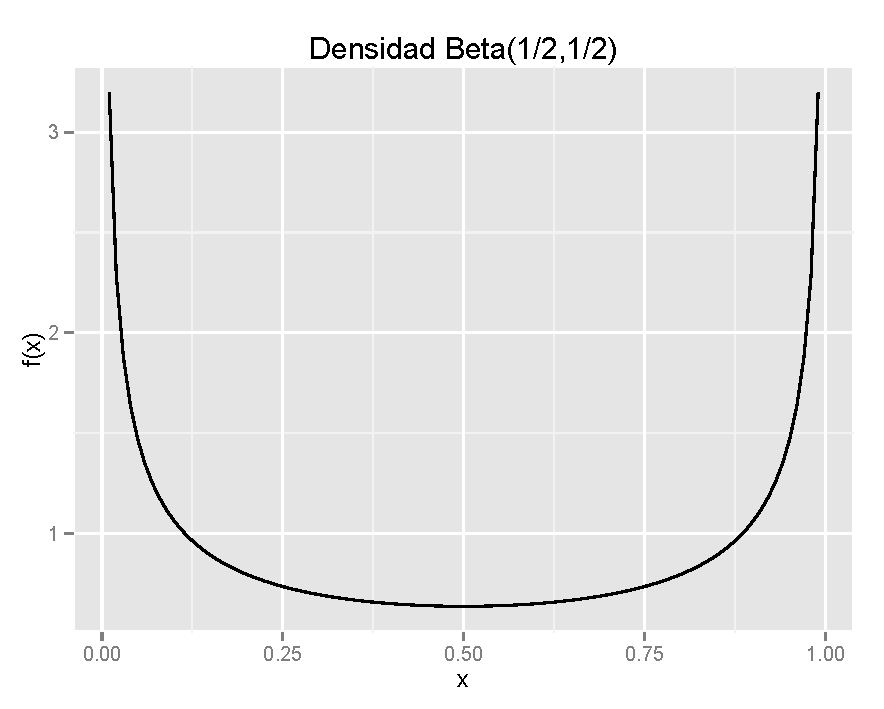
\includegraphics[scale=0.5]{Beta_no_inf.pdf}
    \caption{\emph{Distribuci\'on previa no informativa de Jeffreys para el par\'ametro de una distribuci\'on Bernoulli}}
    \end{figure}
    
    \begin{Res}
    La distribuci\'on predictiva previa para una observaci\'on $y$ est\'a dada por
    \begin{equation}\label{Predi_previa_bernou}
    p(Y)=\frac{Beta(y+\alpha,\beta-y+1)}{Beta(\alpha,\beta)}I_{\{0,1\}}(y),
    \end{equation}
    y define una aut\'entica funci\'on de densidad de probabilidad continua.
    \end{Res}
    
    \begin{proof}
    De la definici\'on de funci\'on de distribuci\'on predictiva se tiene que
    \begin{align*}
    p(Y)&=\int p(Y \mid \theta)p(\theta \mid \alpha,\beta)\ d\theta\\
    &=\int_0^1 \theta^y(1-\theta)^{1-y}I_{\{0,1\}}(y)\frac{1}{Beta(\alpha,\beta)}\theta^{\alpha-1}(1-\theta)^{\beta-1}\ d\theta\\
    &=\frac{Beta(y+\alpha,\beta-y+1)}{Beta(\alpha,\beta)}I_{\{0,1\}}(y)
    \int_0^1\frac{\theta^{y+\alpha-1}(1-\theta)^{\beta-y+1-1}}{Beta(y+\alpha,\beta-y+1)}\ d\theta\\
    &=\frac{Beta(y+\alpha,\beta-y+1)}{Beta(\alpha,\beta)}I_{\{0,1\}}(y)
    \end{align*}
    
    N\'otese que en la anterior demostraci\'on, la integral al lado derecho de la tercera igualdad es igual a la unidad, puesto que la expresi\'on matem\'atica dentro de la integral corresponde a la funci\'on de densidad de una variable aleatoria con distribucion $Beta$, que tiene rango en el intervalo $(0,1)$. Por otro lado se deben verificar las dos condiciones de funci\'on de densidad. Es decir
    \begin{enumerate}
    \item $p(Y)>0 ~(\forall y\in Y)$. Esta condici\'on se tiene trivialmente puesto que la funci\'on matem\'atica Beta siempre toma valores positivos.
    \item $\int p(y)\ dx=1$. En este caso, esta funci\'on es discreta definida en el conjunto $\{0,1\}$. Por lo tanto esta condici\'on es equivalente a
    \begin{equation*}
    \sum_{y\in{\{0,1\}}}P(Y=y)=\sum_{y\in{\{0,1\}}}\frac{Beta(y+\alpha,\beta-y+1)}{Beta(\alpha,\beta)}=1
    \end{equation*}
    Lo cual se verifica f\'acilmente teniendo en cuenta las propiedades de la funci\'on matem\'atica Beta y de la funci\'on matem\'atica Gamma.
    \end{enumerate}
    \end{proof}
    
    La distribuci\'on predictiva dada en \ref{Predi_previa_bernou} est\'a basada \'unicamente en la distribuci\'on previa del par\'ametro $\theta$, una vez observada la variable $Y$ se puede pensar en actualizar la distribuci\'on predictiva basando en la distribuci\'on posterior del par\'ametro, esta distribuci\'on se da en el siguiente resultado.
    
    \begin{Res}
    Despu\'es de la recolecci\'on de los datos, la distribuci\'on predictiva posterior para una nueva observaci\'on $\tilde{y}$ est\'a dada por
    \begin{equation}
    p(\tilde{y} \mid Y)=\frac{Beta(\tilde{y}+y+\alpha,\beta-\tilde{y}-y+2)}{Beta(y+\alpha,\beta-y+1)}I_{\{0,1\}}(\tilde{y}),
    \end{equation}
    \end{Res}
    
    \begin{proof}
    De la definici\'on de funci\'on de distribuci\'on predictiva se tiene que
    \begin{align*}
    p(\tilde{y} \mid Y)&=\int p(\tilde{y} \mid \theta)p(\theta \mid Y)\ d\theta\\
    &=\int_0^1\theta^{\tilde{y}}(1-\theta)^{1-\tilde{y}}I_{\{0,1\}}(\tilde{y})
    \frac{\theta^{y+\alpha-1}(1-\theta)^{\beta-y+1-1}}{Beta(y+\alpha,\beta-y+1)}\ d\theta\\
    &=\frac{Beta(\tilde{y}+y+\alpha,\beta-\tilde{y}-y+2)}{Beta(y+\alpha,\beta-y+1)}I_{\{0,1\}}(\tilde{y})\\
    &\hspace{2cm}\times \int_0^1\frac{\theta^{\tilde{y}+y+\alpha-1}(1-\theta)^{\beta-\tilde{y}-y+2-1}}
    {Beta(\tilde{y}+y+\alpha,\beta-\tilde{y}-y+2)}\ d\theta\\
    &=\frac{Beta(\tilde{y}+y+\alpha,\beta-\tilde{y}-y+2)}{Beta(y+\alpha,\beta-y+1)}I_{\{0,1\}}(\tilde{y})
    \end{align*}
    \end{proof}
    
    Ahora, en la pr\'actica rara vez se observa la realizaci\'on de una \'unica variable aleatoria Bernoulli $Y$, sino una muestra de variables aleatorias $Y_1$, $\cdots$, $Y_n$. En este caso, la distribuci\'on posterior del par\'ametro $\theta$ est\'a dada en el siguiente resultado.
    
    \begin{Res}
    Cuando se tiene una muestra aleatoria $Y_1,\ldots,Y_n$ de variables con distribuci\'on Bernoulli de par\'ametro $\theta$, entonces la distribuci\'on posterior del par\'ametro de inter\'es es
    \begin{equation*}
    \theta \mid Y_1,\ldots,Y_n \sim Beta\left(\sum_{i=1}^ny_i+\alpha,\beta-\sum_{i=1}^ny_i+n\right)
    \end{equation*}
    \end{Res}
    
    La demostraci\'on se deja como ejercicio.
    
    \begin{Eje}
    Es com\'un en muchos pa\'ises del mundo que se presenten encuestas de opini\'on electoral unas semanas antes de las elecciones presidenciales. Dentro de este tipo de encuestas se acostumbra a indagar acerca del favoritismo de los candidatos involucrados en la contienda electoral. Suponga que un candidato presidencial llamado Jos\'e P\'erez est\'a interesado en conocer su intenci\'on de voto previa a las elecciones. Para esto, \'el contrata a una firma encuestadora para la realizaci\'on de un muestreo probabil\'istico entre la poblaci\'on votante. El resultado de este estudio puede hacer cambiar o afirmar las estrategias publicitarias y la redefinici\'on de la campa\~na electoral. La firma encuestadora decide implementar una estrategia de muestreo con un tama\~no de muestra de doce mil personas. A cada respondiente se le realiza la siguiente pregunta: \textbf{Si las elecciones presidenciales fueran ma\~nana. ?Usted votar\'ia por el candidato Jos\'e P\'erez?}
    
    Las respuestas a esta pregunta son realizaciones de una muestra aleatoria de doce mil variables con densidad Bernoulli. Los resultados del estudio arrojan que 6360 personas de las personas entrevistadas, es decir un 53 por ciento, votar\'ian por el suscrito candidato. T\'ecnicamente se debe analizar esta cifra puesto que las implicaciones de ganar en una primera vuelta son grandes en el sentido econ\'omico, log\'istico y administrativo. Claramente, el dato 53 por ciento asegura una ventaja dentro de la muestra de doce mil personas. Sin embargo, es necesario realizar un estudio m\'as profundo acerca de la caracterizaci\'on estructural de la intenci\'on de voto del candidato en la poblaci\'on de todos los votantes.
    
    Con base en lo anteriormente expuesto, se decide utilizar la inferencia bayesiana puesto que existe informaci\'on previa de un estudio anterior, contratado por el mismo candidato unos meses atr\'as en donde se entrevistaron a mil personas, con un favoritismo que estaba alrededor del 35 por ciento. Esta situaci\'on conlleva a la utilizaci\'on de la metodolog\'ia bayesiana que incorpora la informaci\'on pasada acerca del mismo fen\'omeno.
    
    El estad\'istico de la firma encuestadora decide utilizar una distribuci\'on previa\footnote{Como se ver\'a m\'as adelante, es conveniente definir los par\'ametros de la distribuci\'on previa como $\alpha$ igual al n\'umero de votantes a favor y $\beta$ igual al n\'umero de votantes en contra.} $Beta(\alpha=350, \beta=650)$. Utilizando el resultado 2.1.4, se contempla que la distribuci\'on posterior del par\'ametro de inter\'es, que representa la probabilidad de \'exito en las elecciones presidenciales, es $Beta(6360+350, 650-6360+12000)=Beta(6710, 6290)$. Por lo tanto, utilizando la distribuci\'on posterior, se estima que la intenci\'on de voto por el candidato es de $\frac{6710}{6710+6290}=\frac{6710}{13000}=0.516$ y este valor equivale a la media de la distribuci\'on posterior. Este mismo an\'alisis puede ejecutarse en \texttt{JAGS}, mediante el uso del siguiente c\'odigo computacional
    
    Sin embargo, si no se tuviese informaci\'on previa como la suministrada por el estudio de meses anteriores, el an\'alisis bayesiano sugerir\'ia trabajar con una distribuci\'on previa no informativa, que en este caso, corresponder\'ia a una $Beta(\alpha=0.5, \beta=0.5)$. siguiendo el mismo an\'alisis, se tiene que la distribuci\'on posterior es $Beta(6360.5, 5640.5)$. Finalmente, se estimar\'ia que la intenci\'on de voto por el candidato es de $\frac{6350.5}{12001}=0.529$. Las figuras \ref{BernoEj1} y \ref{BernoEj2} muestran el comportamiento de las distribuciones previas y posteriores en ambos escenarios. N\'otese que la distribuci\'on no informativa influye muy poco en el comportamiento de la distribuci\'on posterior.
    
    \begin{figure}[!h]
    \centering
    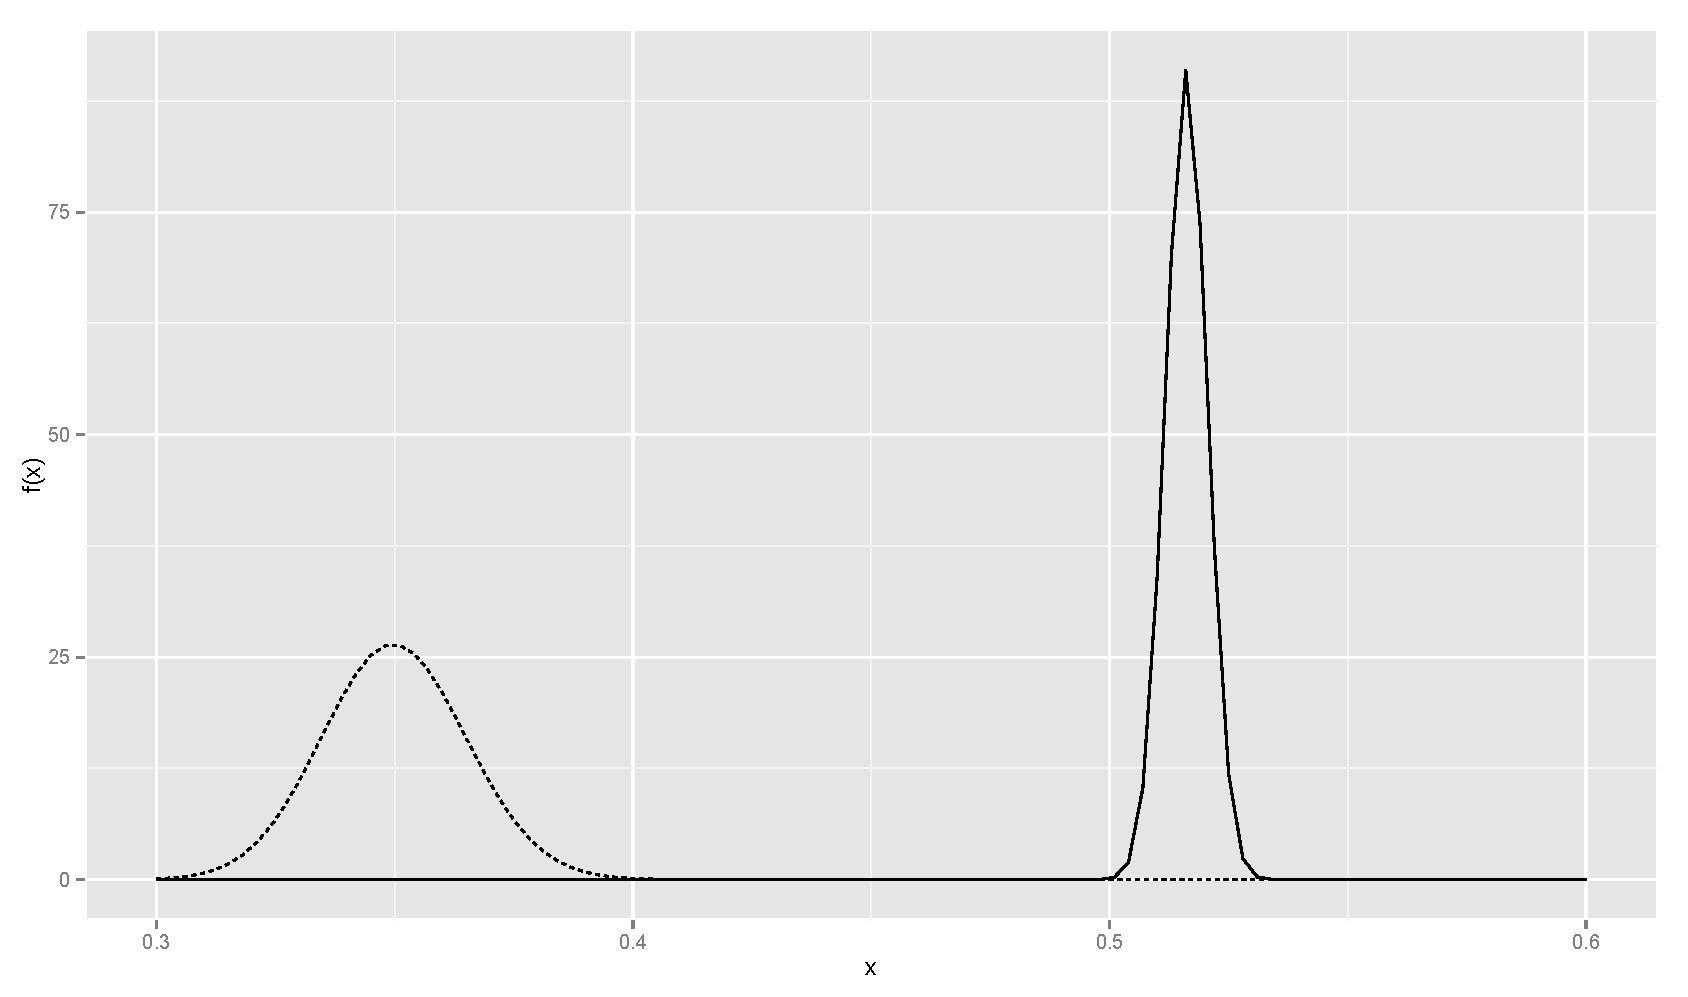
\includegraphics[scale=0.28]{BernoEj1.pdf}
    \caption{\emph{Distribuci\'on previa informativa (l\'inea punteada) y distribuci\'on posterior (l\'inea s\'olida) para el ejemplo de las encuestas electorales.}}
    \label{BernoEj1}
    \end{figure}
    
    \begin{figure}[!h]
    \centering
    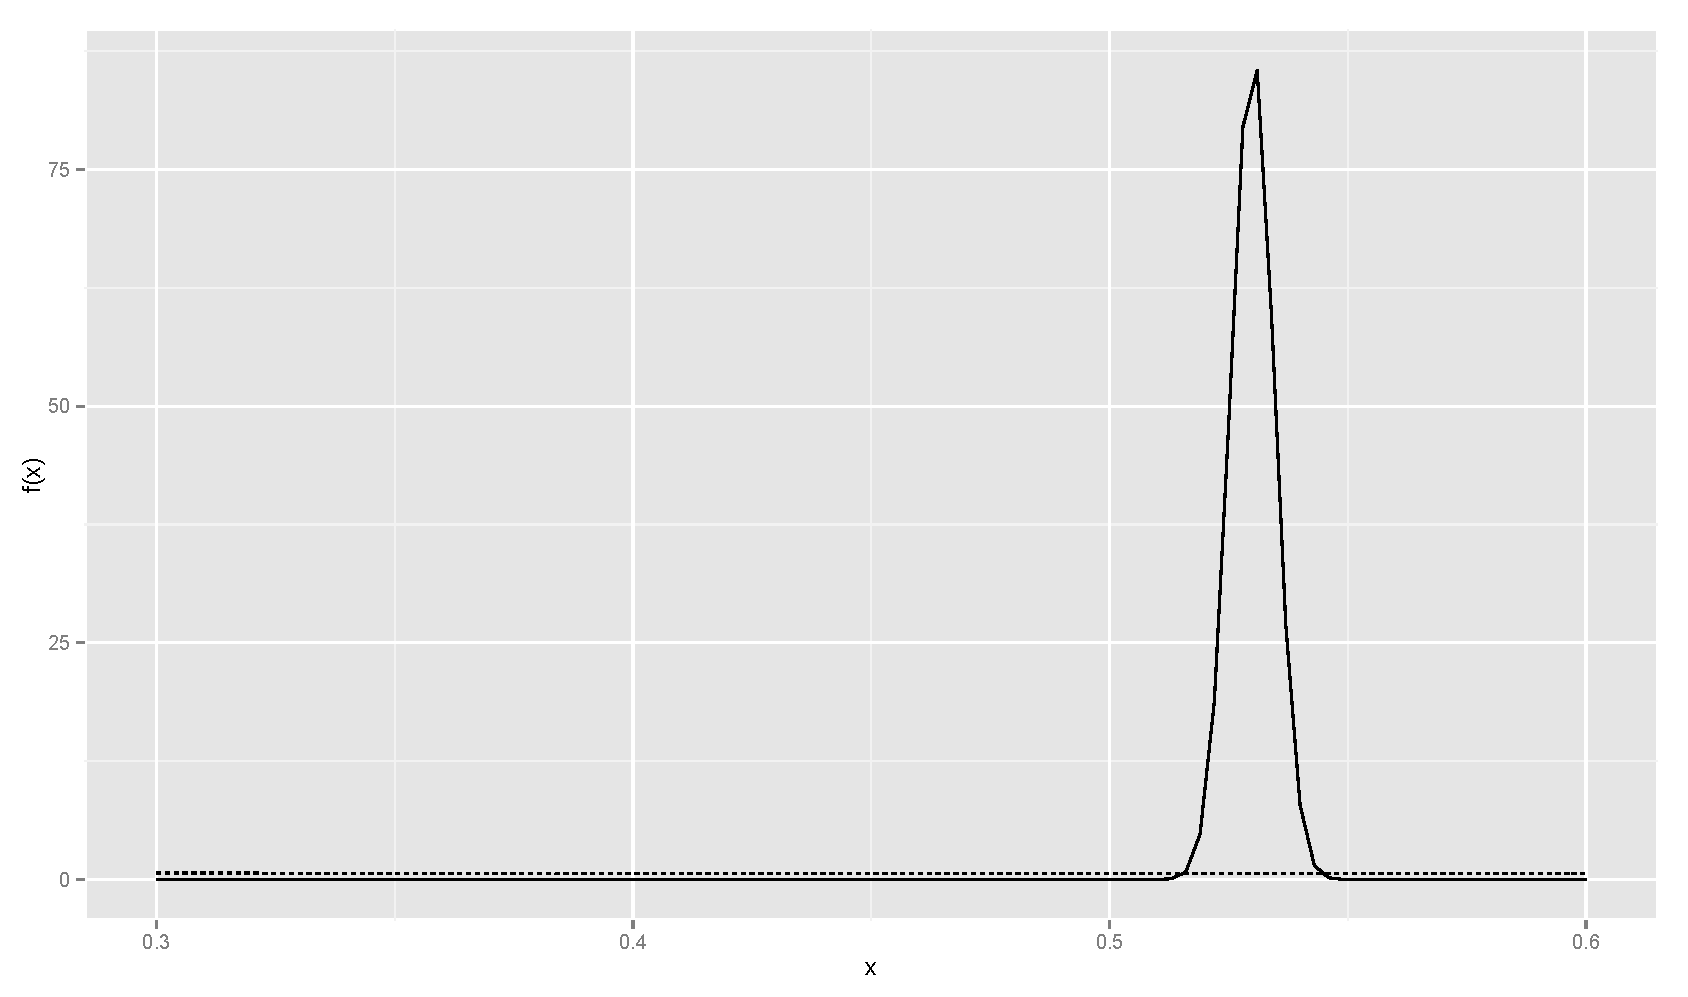
\includegraphics[scale=0.28]{BernoEj2.pdf}
    \caption{\emph{Distribuci\'on previa no informativa (l\'inea punteada) y distribuci\'on posterior (l\'inea s\'olida) para el ejemplo de las encuestas electorales.}}
    \label{BernoEj2}
    \end{figure}
    
    Utilizando el siguiente c\'odigo en R, es posible conocer los intervalos de credibilidad para las dos distribuciones posteriores. Es posible concluir que en ambos escenarios, el candidato aventaja significativamente a sus contrincantes y, salvo alg\'un cambio dr\'astico en el comportamiento del electorado, ganar\'a las elecciones. Lo anterior se deduce puesto que el intervalo de credibilidad al 95\% no contiene ning\'un valor menor a 0.5
    
\begin{knitrout}
\definecolor{shadecolor}{rgb}{0.933, 0.933, 0.933}\color{fgcolor}\begin{kframe}
\begin{alltt}
\hlkwd{qbeta}\hlstd{(}\hlkwd{c}\hlstd{(}\hlnum{0.025}\hlstd{,} \hlnum{0.975}\hlstd{),} \hlnum{6710}\hlstd{,} \hlnum{6290}\hlstd{)}
\end{alltt}
\begin{verbatim}
## [1] 0.5076 0.5247
\end{verbatim}
\begin{alltt}
\hlkwd{qbeta}\hlstd{(}\hlkwd{c}\hlstd{(}\hlnum{0.025}\hlstd{,}\hlnum{0.975}\hlstd{),} \hlnum{6350.5}\hlstd{,} \hlnum{5640.5}\hlstd{)}
\end{alltt}
\begin{verbatim}
## [1] 0.5207 0.5385
\end{verbatim}
\end{kframe}
\end{knitrout}

    Por otro lado, el siguiente c\'odigo en JAGS permite obtener el mismo tipo de inferencia creando tres cadenas de Markov cuya distribuci\'on de probabilidad coincide con la distribuci\'on posterior del ejemplo.
    
\begin{knitrout}
\definecolor{shadecolor}{rgb}{0.933, 0.933, 0.933}\color{fgcolor}\begin{kframe}
\begin{alltt}
\hlcom{# Datos}
\hlstd{y} \hlkwb{<-} \hlkwd{c}\hlstd{(}\hlnum{1}\hlstd{,} \hlnum{0}\hlstd{,} \hlnum{1}\hlstd{,...,} \hlnum{0}\hlstd{)}
\hlstd{n} \hlkwb{<-}\hlkwd{length}\hlstd{(y)}

\hlcom{# Modelo Bernoulli}
\hlstd{Bern.model} \hlkwb{<-}\hlkwa{function}\hlstd{() \{}
\hlkwa{for}\hlstd{(i} \hlkwa{in} \hlnum{1}\hlopt{:}\hlstd{n)}
\hlstd{\{}
\hlstd{y[i]}\hlopt{~}\hlkwd{dbern}\hlstd{(theta)}
\hlstd{\}}
\hlstd{theta}\hlopt{~}\hlkwd{dbeta}\hlstd{(}\hlnum{350}\hlstd{,} \hlnum{650}\hlstd{)}
\hlstd{\}}

\hlstd{bern.data} \hlkwb{<-} \hlkwd{list}\hlstd{(}\hlstr{"y"}\hlstd{,}\hlstr{"n"}\hlstd{)}
\hlstd{bern.param} \hlkwb{<-} \hlkwd{c}\hlstd{(}\hlstr{"theta"}\hlstd{)}
\hlstd{bern.inits} \hlkwb{<-} \hlkwa{function}\hlstd{()\{}\hlkwd{list}\hlstd{(}\hlstr{"theta"}\hlstd{=}\hlkwd{c}\hlstd{(}\hlnum{0.5}\hlstd{))\}}
\hlkwd{set.seed}\hlstd{(}\hlnum{123}\hlstd{)}

\hlstd{bern.fit} \hlkwb{<-} \hlkwd{jags}\hlstd{(}\hlkwc{data}\hlstd{=bern.data,} \hlkwc{inits}\hlstd{=bern.inits, bern.param,}
\hlkwc{n.chains}\hlstd{=}\hlnum{3}\hlstd{,} \hlkwc{n.iter}\hlstd{=}\hlnum{10000}\hlstd{,} \hlkwc{n.burnin}\hlstd{=}\hlnum{1000}\hlstd{,} \hlkwc{n.thin}\hlstd{=}\hlnum{10}\hlstd{,} \hlkwc{model.file}\hlstd{=bern.model)}

\hlkwd{print}\hlstd{(bern.fit)}
\end{alltt}
\end{kframe}
\end{knitrout}
    \end{Eje}
    
    \section{Modelo Binomial}
    
    Cuando se dispone de una muestra aleatoria de variables con distribuci\'on Bernoulli $Y_1,\ldots,Y_n$, la inferencia bayesiana se puede llevar a cabo usando la distribuci\'on Binomial, puesto que es bien sabido que la suma de variables aleatorias Bernoulli
    \begin{equation*}
    S=\sum_{i=1}^nY_i
    \end{equation*}
    sigue una distribuci\'on Binomial. Es decir:
    \begin{equation}
    p(S \mid \theta)=\binom{n}{s}\theta^s(1-\theta)^{n-s}I_{\{0,1,\ldots,n\}}(s),
    \end{equation}
    
    N\'otese que la distribuci\'on binomial es un caso general para la distribuci\'on Bernoulli, cuando $n=1$. Entonces, as\'i como en la distribuci\'on Bernoulli, el par\'ametro $\theta$ est\'a restringido al espacio $\Theta=[0,1]$. Luego, es admisible proponer que $\theta$ siga una distribuci\'on Beta. Por tanto la distribuci\'on previa del par\'ametro $\theta$ est\'a dada por la expresi\'on (2.1.2). Bajo este marco de referencia se tienen los siguientes resultados
    
    \begin{Res}
    La distribuci\'on posterior del par\'ametro $\theta$ sigue una distribuci\'on
    \begin{equation*}
    \theta \mid S \sim Beta(s+\alpha,\beta-s+n)
    \end{equation*}
    \end{Res}
    
    \begin{proof}
    \begin{align*}
    p(\theta \mid S)&\propto p(S \mid \theta)p(\theta \mid \alpha,\beta)\\
    &=\frac{\binom{n}{s}I_{\{0,1,\ldots,n\}}(s)}{Beta(\alpha,\beta)}
    \theta^s\theta^{\alpha-1} (1-\theta)^{\beta-1}(1-\theta)^{n-s}I_{[0,1]}(\theta)\\
    &\propto \theta^{s+\alpha-1} (1-\theta)^{\beta-s+n-1}I_{[0,1]}(\theta)
    \end{align*}
    Por lo tanto, factorizando convenientemente, se llega a una expresi\'on id\'entica a la funci\'on de distribuci\'on de una variable aleatoria con distribuci\'on $Beta(s+\alpha,\beta-s+n)$.
    
    \end{proof}
    
    Del resultado anterior podemos ver que el estimador bayesiano de $\theta$ est\'a dada por la media de la distribuci\'on posterior, dada por
    \begin{equation}\label{esti_beta}
    \hat{\theta}_{B}=\frac{s+\alpha}{n+\alpha+\beta}
    \end{equation}
    
    En la pr\'actica, se acostumbra a escoger los hiperpar\'ametros $\alpha$ y $\beta$ de tal forma que correspondan al n\'umero de \'exitos y fracasos obtenidos en los datos previa, respectivamente. De esta forma, $\hat{\theta}_{P}=\alpha/(\alpha+\beta)$ corresponde a la estimaci\'on previa del par\'ametro $\theta$. Por otro lado, el estimador cl\'asico de $\theta$ est\'a dado por $\hat{\theta}_{C}=s/n$. Entonces es posible notar que el estimador bayesiano de $\theta$ en (\ref{esti_beta}) de alguna forma combina el estimador cl\'asico y el estimador previa. M\'as a\'un, se puede ver que $\hat{\theta}_{B}$ se puede escribir como un promedio ponderado entre la estimaci\'on cl\'asica y la estimaci\'on previa. Puesto que
    \begin{align*}
    \hat{\theta}_{B}=\frac{s+\alpha}{n+\alpha+\beta}&=\frac{s}{n+\alpha+\beta}+\frac{\alpha}{n+\alpha+\beta}\\
    &=\frac{n}{n+\alpha+\beta}\frac{s}{n}+\frac{\alpha+\beta}{n+\alpha+\beta}\frac{\alpha}{\alpha+\beta}\\
    &=\frac{n}{n+\alpha+\beta}\hat{\theta}_{C}+\frac{\alpha+\beta}{n+\alpha+\beta}\hat{\theta}_{P}
    \end{align*}
    
    De esta forma, queda en evidencia que la estimaci\'on bayesiana de $\theta$ siempre ser\'a un valor intermedio entre la estimaci\'on cl\'asica y la estimaci\'on previa. La gr\'afica \ref{beta3} da una ilustraci\'on acerca de la anterior afirmaci\'on, en donde se puede observar que para una distribuci\'on previa concentrada en $2/7$ y una funci\'on de verosimilitud\footnote{La funci\'on de verosimilitud es una funci\'on del par\'ametro y s\'olo se puede graficar una vez se hayan observado las realizaciones de la variable aleatoria.} con m\'aximo en $8/10$, se tiene una distribuci\'on posterior centrada en $10/17$; es decir, la estimaci\'on bayesiana se encuentra situada entre la estimaci\'on previa y la estimaci\'on cl\'asica.
    
    \begin{figure}[!h]
    \centering
    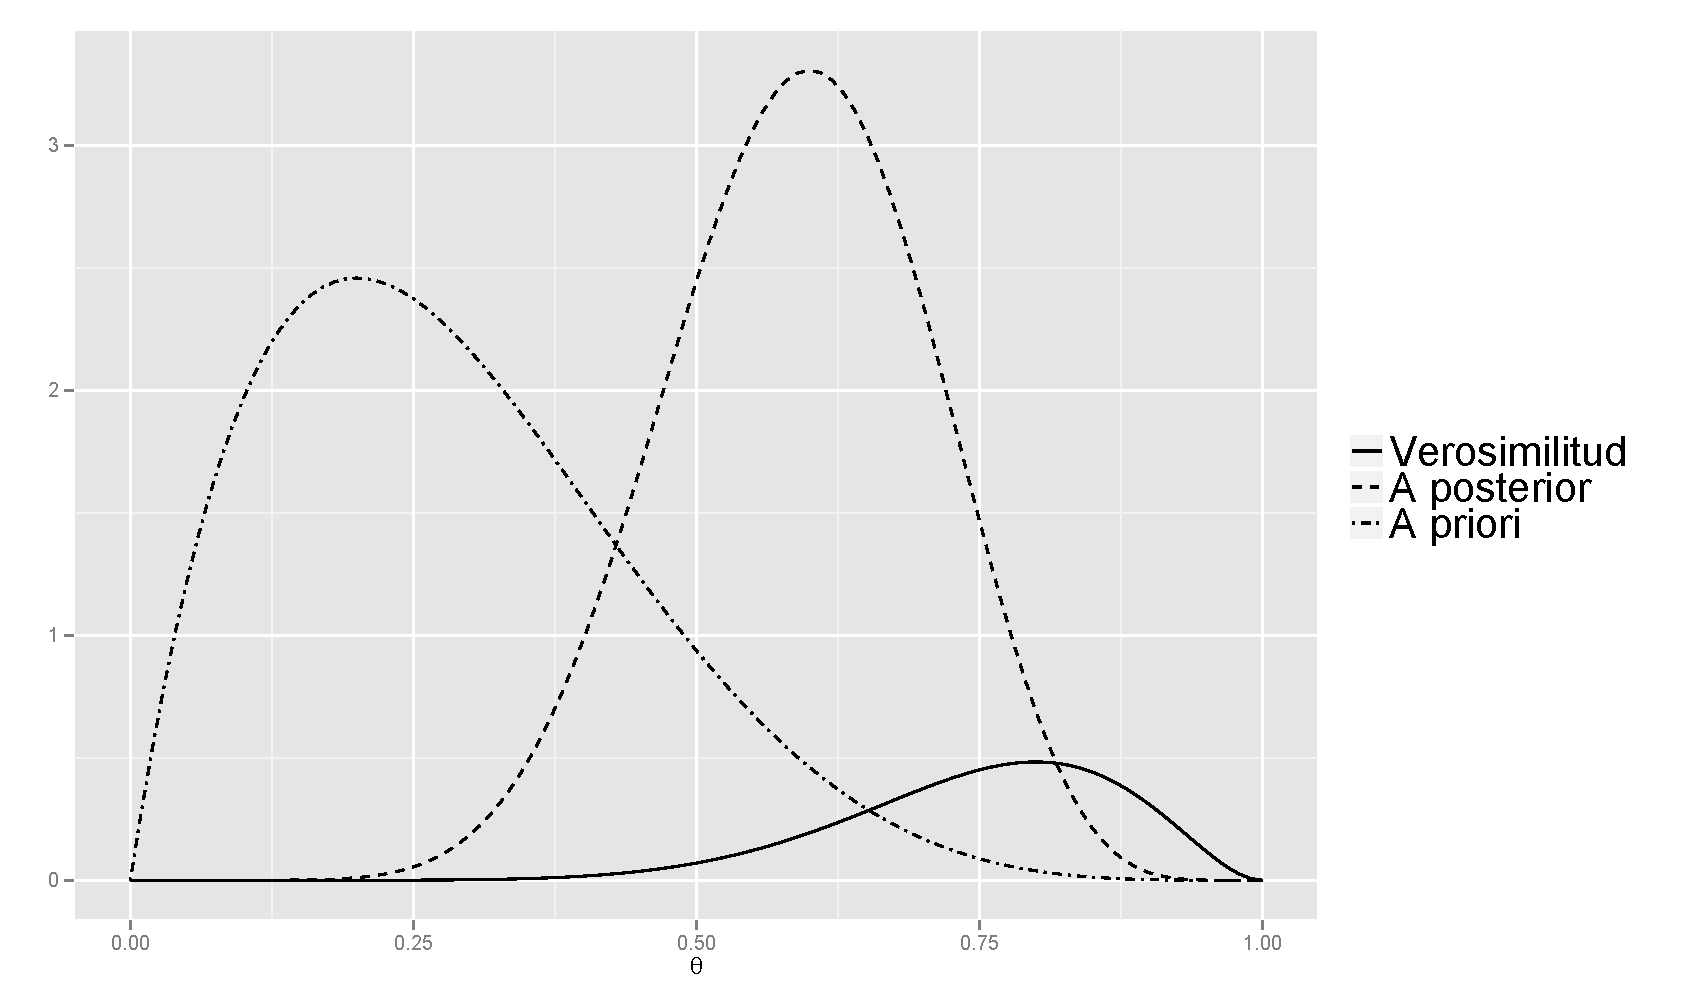
\includegraphics[scale=0.4]{Beta_tres.pdf}
    \caption{\emph{Funci\'on de verosimilitud, funci\'on de densidad previa y posterior para $\alpha=2$, $\beta=5$, $s=8$ y $n=10$.}}
    \label{beta3}
    \end{figure}
    
    Por otro lado, entre m\'as grande sea el tama\~no muestral $n$, m\'as cercano estar\'a $\hat{\theta}_{B}$ de $\hat{\theta}_{C}$ o equivalentemente la funci\'on de densidad posterior de $\theta$ estar\'a m\'as concentrada en $s/n$; mientras que entre mayor n\'umero de datos tenga la muestra de la distribuci\'on previa ($\alpha+\beta$=n\'umero de datos), m\'as cercano estar\'a $\hat{\theta}_{B}$ de $\hat{\theta}_{P}$ y la densidad posterior de $\theta$ estar\'a m\'as concentrada en $\alpha/(\alpha+\beta)$.
    
    Para ilustrar lo anterior, suponga que la distribuci\'on previa de $\theta$ est\'a dada con $\alpha=\beta=5$, es decir la estimacion previa es 0.5, y suponga adem\'as que la estimaci\'on cl\'asica es 0.33, pero el tama\~no muestral $n$ incrementa manteniendo constante la estimacion cl\'asica. En la figura \ref{betan} se muestra la estimaci\'on posterior de $\theta$, es evidente que a medida que el tama\~no muestral $n$ aumenta, la estimaci\'on posterior se acerca m\'as a la estimaci\'on cl\'asica.
    
    \begin{figure}[!h]
    \centering
    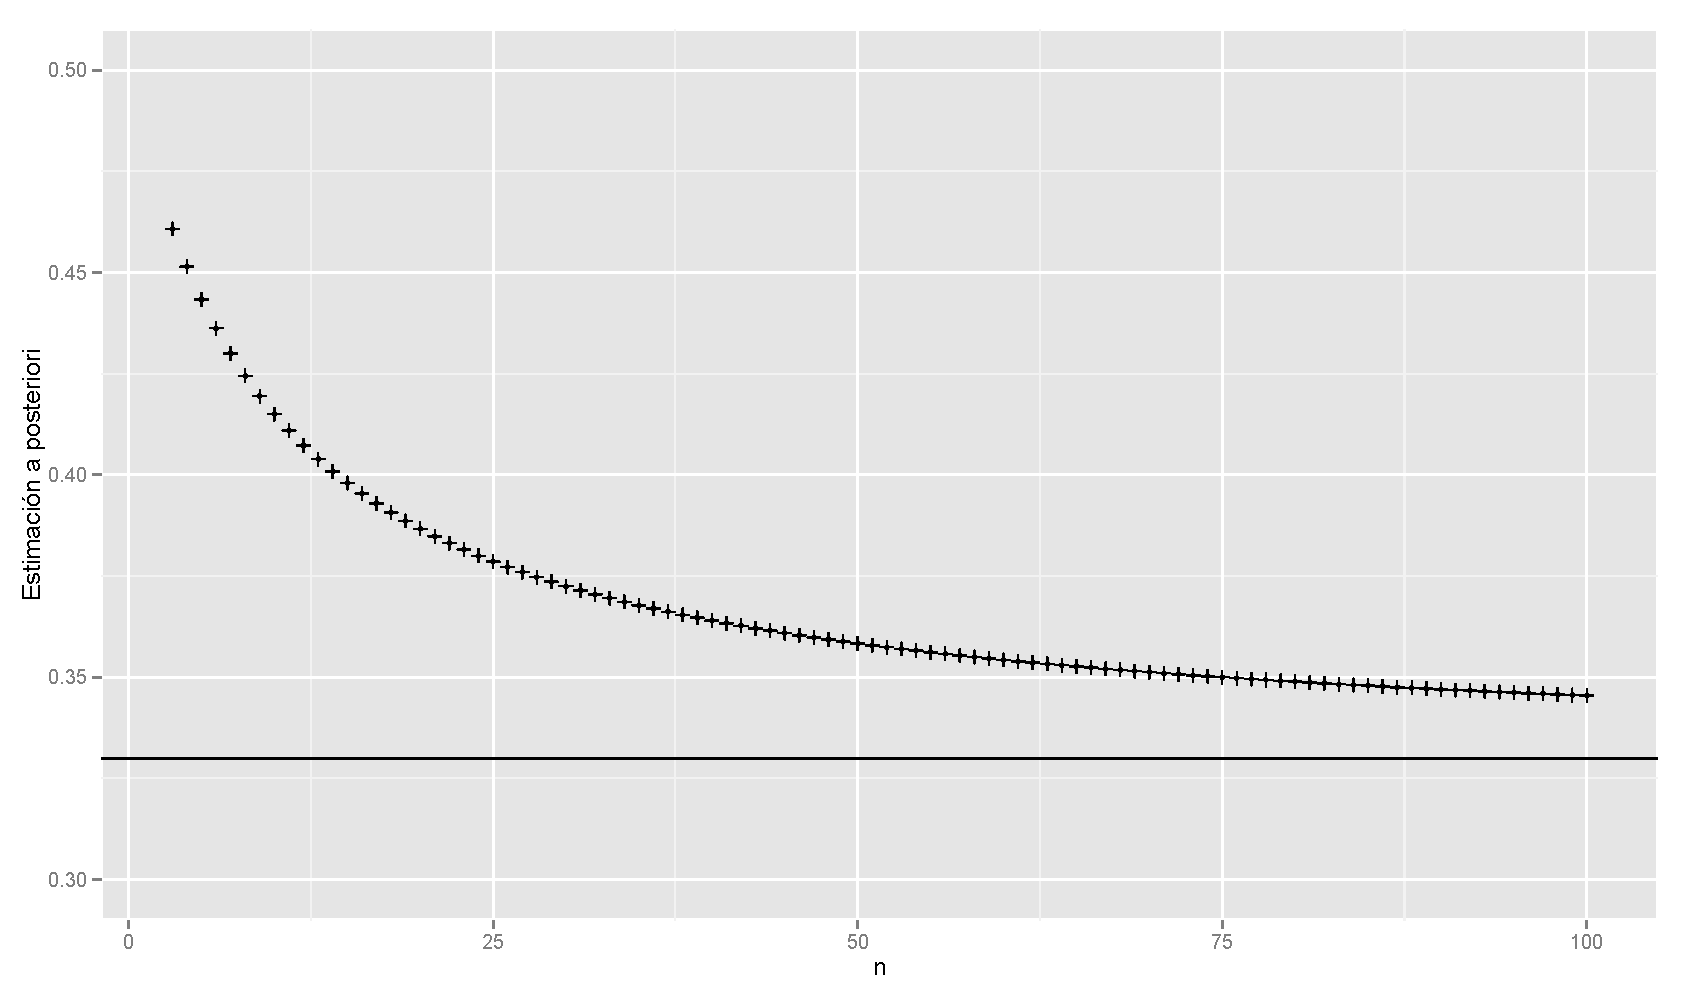
\includegraphics[scale=0.35]{Beta_n_aumen.pdf}
    \caption{\emph{Estimaci\'on posterior de $\theta$ para diferentes valores de $n$ y $s$ con $\alpha=\beta=5$.}}
    \label{betan}
    \end{figure}
    
    Anteriormente, se coment\'o que se acostumbra a escoger los par\'ametros $\alpha$ y $\beta$ que correspondan al n\'umero de \'exitos y fracasos en la informaci\'on previa, sin embargo, la informaci\'on previa puede no presentarse de esta forma. Por ejemplo, en algunas situaciones, la informaci\'on previa puede proveer el valor de $\theta$, es decir, el valor de $\hat{\theta}_P$, y el valor de la desviaci\'on est\'andar de la estimaci\'on (com\'unmente conocido como el error est\'andar). Por ejemplo, suponga que $\hat{\theta}_P=0.5$ con un error est\'andar de 0.1, entonces podemos encontrar los valores de $\alpha$ y $\beta$ de las expresiones $\frac{\alpha}{\alpha+\beta}=0.5$ y $\sqrt{\frac{\alpha\beta}{(\alpha+\beta)^2(\alpha+\beta+1)}}=0.1$, de donde se tiene que $\alpha=12$ y $\beta=12$, y la distribuci\'on a priori correspondiente $Beta(12,12)$ tiene una esperanza de 0.05 y una desviaci\'on est\'andar de 0.1. Se puede ver que entre mayor sea la desviaci\'on est\'andar, menores resultan los valores de $\alpha$ y $\beta$, que conducen a una distribuci\'on previa menos informativa.
    
    Ahora, se vio anteriomente que la distribuci\'on previa no informativa de Jeffreys corresponde a la distribuci\'on $Beta(1/2,1/2)$, la cual conduce a la distribuci\'on posterior $Beta(s+1/2,n-s+1/2)$, que a su vez nos lleva al estimador 
    \begin{equation}
    \label{Esti_theta_Jeffreys}
    \hat{\theta}_B=\frac{s+1/2}{n+1}
    \end{equation}
    
    La anterior expresi\'on es comparable con el estimador cl\'asico $\hat{\theta_C}=\frac{s}{n}$, en el sentido de que los dos son aplicables cuando no se dispone de ninguna informaci\'on previa. Podemos observar que aparte del alto grado de similitud que tienen los dos estimadores, es preferible usar el estimador (\ref{Esti_theta_Jeffreys}) en situaciones donde el valor te\'orico de $\theta$ es muy peque\~no, y como consecuencia en la muestra $s=0$, por ejemplo, cuando $\theta$ representa el porcentaje de personas que esten infectados con alg\'un virus poco com\'un. En estos casos, el estimador cl\'asico $\hat{\theta}_C=0$ sugiriendo que ning\'un porcentaje de la poblaci\'on est\'a infectado, conclusi\'on que puede ser err\'onea; por otro lado, el estimador bayesiano $\hat{\theta}_B=\frac{0.5}{n+1}$, el cual tiende a ser un porcentaje muy peque\~no a medida que aumente el tama\~no muestral $n$, pero nunca llega a dar el valor 0 como la estimaci\'on de $\theta$.
    
    En el siguiente resultado, se encuentra la distribuci\'on predictiva previa para una variable binomial $S$.
    
    \begin{Res}
    La distribuci\'on predictiva previa para la observaci\'on particular de la suma de variables aleatorias Bernoulli, $s$, est\'a dada por una distribuci\'on Beta-Binomial dada por
    \begin{equation}
    p(S)=\binom{n}{s}\frac{Beta(s+\alpha,\beta-s+n)}{Beta(\alpha,\beta)}I_{\{0,1,\ldots,n\}}(s).
    \end{equation}
    \end{Res}
    
    \begin{proof}
    De la definici\'on de funci\'on de distribuci\'on predictiva previa se tiene que
    \begin{align*}
    p(S)&=\int p(S \mid \theta)p(\theta \mid \alpha,\beta)\ d\theta\\
    &=\int_0^1\binom{n}{s}\theta^s(1-\theta)^{n-s}I_{\{0,1,\ldots,n\}}(s)
    \frac{1}{Beta(\alpha,\beta)}\theta^{\alpha-1}(1-\theta)^{\beta-1}\ d\theta\\
    &=\binom{n}{s}\frac{Beta(s+\alpha,\beta-s+n)}{Beta(\alpha,\beta)}I_{\{0,1,\ldots,n\}}(s)\\
    &\hspace{2cm}\times\int_0^1\frac{\theta^{s+\alpha-1}(1-\theta)^{\beta-s+n-1}}{Beta(s+\alpha,\beta-s+n)}\ d\theta\\
    &=\binom{n}{s}\frac{Beta(s+\alpha,\beta-s+n)}{Beta(\alpha,\beta)}I_{\{0,1,\ldots,n\}}(s)
    \end{align*}
    \end{proof}
    
    
    Una vez observados los valores muestrales, podemos encontrar la distribuci\'on predictiva posterior para una nueva variable binomial $\tilde{S}$ en una muestra de tama\~no $\tilde{n}$. Esta distribuci\'on se encuentra en el siguiente resultado.
    \begin{Res}
    \label{ResPredBinom}
    Despu\'es de la recolecci\'on de los datos $y_1$, $\cdots$, $y_n$, la distribuci\'on predictiva posterior para una nueva variable $\tilde{S}$ en una muestra del tama\~no $\tilde{n}$ est\'a dada por
    \begin{equation}\label{Binom_predict}
    p(\tilde{s} \mid S)=\binom{\tilde{n}}{\tilde{s}}\frac{Beta(\tilde{s}+s+\alpha,\beta-\tilde{s}-s+n+\tilde{n})}{Beta(s+\alpha,\beta-s+n)}I_{\{0,1,\ldots,\tilde{n}\}}(\tilde{s}),
    \end{equation}
    \end{Res}
    
    \begin{proof}
    De la definici\'on de funci\'on de distribuci\'on predictiva se tiene que
    \begin{align*}
    p(\tilde{s} \mid S)&=\int p(\tilde{s} \mid \theta)p(\theta \mid S)\ d\theta\\
    &=\int_0^1 \binom{\tilde{n}}{\tilde{s}} \theta^{\tilde{s}}(1-\theta)^{\tilde{n}-\tilde{s}}I_{\{0,1,\ldots,\tilde{n}\}}(\tilde{s})
    \frac{\theta^{s+\alpha-1}(1-\theta)^{\beta-s+n-1}}{Beta(s+\alpha,\beta-s+n)}\ d\theta\\
    &=\binom{\tilde{n}}{\tilde{s}}\frac{Beta(\tilde{s}+s+\alpha,\beta-\tilde{s}-s+n+\tilde{n})}{Beta(s+\alpha,\beta-s+n)}I_{\{0,1,\ldots,\tilde{n}\}}(\tilde{s})\\
    & \hspace{2cm}\times
    \int_0^1\frac{\theta^{\tilde{s}+s+\alpha-1}(1-\theta)^{\beta-\tilde{s}-s+n+\tilde{n}-1}}
    {Beta(\tilde{s}+s+\alpha,\beta-\tilde{s}-s+n+\tilde{n})}\ d\theta\\
    &=\binom{\tilde{n}}{\tilde{s}}\frac{Beta(\tilde{s}+s+\alpha,\beta-\tilde{s}-s+n+\tilde{n})}{Beta(s+\alpha,\beta-s+n)}I_{\{0,1,\ldots,\tilde{n}\}}(\tilde{s})
    \end{align*}
    \end{proof}
    
    En la anterior distribuci\'on predictiva, se necesita calcular funciones Beta. Cuando los tama\~nos muestrales $n$, $\tilde{n}$ y/o los par\'ametros de la distribuci\'on previa $\alpha$ y $\beta$ son muy grandes, puede presentar problemas num\'ericos al momento de calcular directamente estas funciones Beta. Por ejemplo, supongamos que $n=1000$, $s=650$, $\alpha=200$, $\beta=300$ y $\tilde{n}=800$, de esta forma, los posibles valores para $\tilde{s}$ son $0,1,\cdots,800$, y se tiene que la probabilidad de que $\tilde{s}$ tome el valor 500 est\'a dada por
    \begin{equation}\label{Eje_binom}
    Pr(\tilde{s}=500|S)=\binom{800}{500}\frac{Beta(1350,950)}{Beta(850,650)}
    \end{equation}
    
    y desafortunadamente, al evaluar \texttt{beta(1350,950)} y \texttt{beta(850,650)} en \textsf{R} da el valor de 0 para ambas expresiones. Planteamos la siguiente soluci\'on num\'erica cuando se quiere calcular la funci\'on predictiva (\ref{Binom_predict}) en muestras grandes. El problema central es el c\'omputo de $\frac{Beta(a,b)}{Beta(c,d)}$ con $a\geq c$ y $b\geq d$, valores enteros. Podemos ver que
    
    \begin{align*}
    &\ \ \ \ \frac{Beta(a,b)}{Beta(c,d)}\\
    &=\frac{(a-1)!(b-1)!(c+d-1)!}{(c-1)!(d-1)!(a+b-1)!}\\
    &=\frac{(a-1)(a-2)\cdots(a-(a-c))(b-1)(b-2)\cdots(b-(b-d))}{(a+b-1)(a+b-2)\cdots(a+b-(a+b-c-d))}\\
    &=\frac{a^{a-c}(1-\frac{1}{a})(1-\frac{2}{a})\cdots(1-\frac{a-c}{a})b^{b-d}(1-\frac{1}{b})(1-\frac{2}{b})\cdots(1-\frac{b-d}{b})}{(a+b)^{a+b-c-d}(1-\frac{1}{a+b})(1-\frac{2}{a+b})\cdots(1-\frac{a+b-c-d}{a+b})}\\
    &=\underbrace{\left(\frac{a}{a+b}\right)^{a-c}}_{t1}\underbrace{\left(\frac{b}{a+b}\right)^{b-d}}_{t2}\underbrace{(1-\frac{1}{a})(1-\frac{2}{a})\cdots(1-\frac{a-c}{a})}_{t3}\\
    &\ \ \ \ \ \ \underbrace{(1-\frac{1}{b})(1-\frac{2}{b})\cdots(1-\frac{b-d}{b})}_{t4}\underbrace{(1-\frac{1}{a+b})(1-\frac{2}{a+b})\cdots(1-\frac{a+b-c-d}{a+b})}_{t5}
    \end{align*}
    
    Calculando separadamente los t\'erminos $t1$, $t2$, $t3$, $t4$ y $t5$ podemos calcular $\frac{Beta(a,b)}{Beta(c,d)}$ para valores grandes de $a$, $b$, $c$ y $d$. La siguiente funci\'on \verb"prob" calcula la densidad (\ref{Binom_predict}) para un valor particular de $\tilde{s}$ usando la anterior t\'ecnica.
    
\begin{knitrout}
\definecolor{shadecolor}{rgb}{0.933, 0.933, 0.933}\color{fgcolor}\begin{kframe}
\begin{alltt}
\hlstd{prob}\hlkwb{<-}\hlkwa{function}\hlstd{(}\hlkwc{s.mono}\hlstd{,}\hlkwc{n.mono}\hlstd{,}\hlkwc{s}\hlstd{,}\hlkwc{n}\hlstd{,}\hlkwc{alfa}\hlstd{,}\hlkwc{beta}\hlstd{)\{}
  \hlstd{a}\hlkwb{<-}\hlstd{s.mono}\hlopt{+}\hlstd{s}\hlopt{+}\hlstd{alfa; b}\hlkwb{<-}\hlstd{n.mono}\hlopt{-}\hlstd{s.mono}\hlopt{+}\hlstd{n}\hlopt{-}\hlstd{s}\hlopt{+}\hlstd{beta}
  \hlstd{c}\hlkwb{<-}\hlstd{s}\hlopt{+}\hlstd{alfa; d}\hlkwb{<-}\hlstd{n}\hlopt{-}\hlstd{s}\hlopt{+}\hlstd{beta}
  \hlstd{t1}\hlkwb{<-}\hlstd{(a}\hlopt{/}\hlstd{(a}\hlopt{+}\hlstd{b))}\hlopt{^}\hlstd{(a}\hlopt{-}\hlstd{c); t2}\hlkwb{<-}\hlstd{(b}\hlopt{/}\hlstd{(a}\hlopt{+}\hlstd{b))}\hlopt{^}\hlstd{(b}\hlopt{-}\hlstd{d)}
  \hlstd{t3}\hlkwb{<-}\hlkwd{prod}\hlstd{(}\hlnum{1}\hlopt{-}\hlkwd{c}\hlstd{(}\hlnum{1}\hlopt{:}\hlstd{(a}\hlopt{-}\hlstd{c))}\hlopt{/}\hlstd{a); t4}\hlkwb{<-}\hlkwd{prod}\hlstd{(}\hlnum{1}\hlopt{-}\hlkwd{c}\hlstd{(}\hlnum{1}\hlopt{:}\hlstd{(b}\hlopt{-}\hlstd{d))}\hlopt{/}\hlstd{b)}
  \hlstd{t5}\hlkwb{<-}\hlkwd{prod}\hlstd{(}\hlnum{1}\hlopt{-}\hlkwd{c}\hlstd{(}\hlnum{1}\hlopt{:}\hlstd{(a}\hlopt{+}\hlstd{b}\hlopt{-}\hlstd{c}\hlopt{-}\hlstd{d))}\hlopt{/}\hlstd{(a}\hlopt{+}\hlstd{b))}
  \hlkwa{if}\hlstd{(a}\hlopt{==}\hlstd{c)\{resul}\hlkwb{<-} \hlstd{t2}\hlopt{*}\hlstd{t4}\hlopt{/}\hlstd{t5\}}
  \hlkwa{if}\hlstd{(b}\hlopt{==}\hlstd{d)\{resul}\hlkwb{<-}\hlstd{t1}\hlopt{*}\hlstd{t3}\hlopt{/}\hlstd{t5\}}
  \hlkwa{if}\hlstd{(a}\hlopt{>}\hlstd{c}\hlopt{&}\hlstd{b}\hlopt{>}\hlstd{d)\{resul}\hlkwb{<-}\hlkwd{choose}\hlstd{(n.mono,s.mono)}\hlopt{*}\hlstd{t1}\hlopt{*}\hlstd{t2}\hlopt{*}\hlstd{t3}\hlopt{*}\hlstd{t4}\hlopt{/}\hlstd{t5\}}
  \hlstd{resul}
\hlstd{\}}
\end{alltt}
\end{kframe}
\end{knitrout}
    
    
    Si queremos examinar la distribuci\'on predictiva para todos valores de la variable $\tilde{S}$, podemos usar los siguientes c\'odigos
\begin{knitrout}
\definecolor{shadecolor}{rgb}{0.933, 0.933, 0.933}\color{fgcolor}\begin{kframe}
\begin{alltt}
\hlstd{n}\hlkwb{<-}\hlnum{1000}\hlstd{; s}\hlkwb{<-}\hlnum{650}
\hlstd{alfa}\hlkwb{<-}\hlnum{200}\hlstd{; beta}\hlkwb{<-}\hlnum{300}
\hlstd{n.mono}\hlkwb{<-}\hlnum{800}
\hlstd{res}\hlkwb{<-}\hlkwd{rep}\hlstd{(}\hlnum{NA}\hlstd{,(}\hlnum{1}\hlopt{+}\hlstd{n.mono))}
\hlkwa{for}\hlstd{(i} \hlkwa{in} \hlnum{1}\hlopt{:}\hlkwd{length}\hlstd{(res))\{}
  \hlstd{res[i]}\hlkwb{<-}\hlkwd{prob}\hlstd{(i}\hlopt{-}\hlnum{1}\hlstd{,n.mono,s,n,alfa,beta)}
\hlstd{\}}
\end{alltt}
\end{kframe}
\end{knitrout}
    
    y como resultado, \verb"res" contiene las 801 probabilidades asociadas a todos los posibles valores de $\tilde{s}$.
    
    Los resultados obtenidos con la anterior t\'ecnica es equivalente a lo obtenido usando la funci\'on \verb"lbeta" que computa el logaritmo natural de la funci\'on beta. As\'i, para calcular la probabilidad en (\ref{Eje_binom}), simplemente usamos el siguiente c\'odigo 
    
\begin{knitrout}
\definecolor{shadecolor}{rgb}{0.933, 0.933, 0.933}\color{fgcolor}\begin{kframe}
\begin{alltt}
\hlkwd{choose}\hlstd{(}\hlnum{800}\hlstd{,}\hlnum{500}\hlstd{)}\hlopt{*}\hlkwd{exp}\hlstd{(}\hlkwd{lbeta}\hlstd{(}\hlnum{1350}\hlstd{,}\hlnum{950}\hlstd{)}\hlopt{-}\hlkwd{lbeta}\hlstd{(}\hlnum{850}\hlstd{,}\hlnum{650}\hlstd{))}
\end{alltt}
\begin{verbatim}
## [1] 0.0005969
\end{verbatim}
\end{kframe}
\end{knitrout}
    N\'otese que esta probabilidad es la misma contenido en \verb"res", puesto que
\begin{knitrout}
\definecolor{shadecolor}{rgb}{0.933, 0.933, 0.933}\color{fgcolor}\begin{kframe}
\begin{alltt}
\hlstd{res[}\hlnum{501}\hlstd{]}
\end{alltt}
\begin{verbatim}
## [1] 0.0005969
\end{verbatim}
\end{kframe}
\end{knitrout}
    Finalmente, se observa que la distribuci\'on predictiva (\ref{Binom_predict}) corresponde a una distribuci\'on Beta-binomial con par\'ametros $s+\alpha$ y $\beta-s+n$. Y el paquete \verb"VGAM" en \verb"R" \cite{VGAM} contiene funciones que calculan la funci\'on de densidad, funci\'on de distribuci\'on, percentiles, adem\'as de generar n\'umeros aleatorios para la distribuci\'on Beta-binomial. Las probabilidades puntuales de $\tilde{s}$ se puede calcular con la funci\'on \verb"dbetabinom", teniendo en cuenta que los par\'ametros utilizados son $\mu=(s+\alpha)/(n+\alpha+\beta)$ y $\rho=1/(1+n+\alpha+\beta)$. Con el siguiente c\'odigo, podemos calcular las probabilidades para todos los posibles valores de $\tilde{s}$.
    
\begin{knitrout}
\definecolor{shadecolor}{rgb}{0.933, 0.933, 0.933}\color{fgcolor}\begin{kframe}
\begin{alltt}
\hlkwd{library}\hlstd{(VGAM)}
\hlstd{mu}\hlkwb{<-}\hlstd{(s}\hlopt{+}\hlstd{alfa)}\hlopt{/}\hlstd{(n}\hlopt{+}\hlstd{alfa}\hlopt{+}\hlstd{beta)}
\hlstd{rho}\hlkwb{<-}\hlnum{1}\hlopt{/}\hlstd{(}\hlnum{1}\hlopt{+}\hlstd{n}\hlopt{+}\hlstd{alfa}\hlopt{+}\hlstd{beta)}
\hlstd{res2}\hlkwb{<-}\hlkwd{rep}\hlstd{(}\hlnum{NA}\hlstd{,(}\hlnum{1}\hlopt{+}\hlstd{n.mono))}
\hlkwa{for}\hlstd{(i} \hlkwa{in} \hlnum{1}\hlopt{:}\hlkwd{length}\hlstd{(res2))\{}
  \hlstd{res2[i]}\hlkwb{<-}\hlkwd{dbetabinom}\hlstd{(i}\hlopt{-}\hlnum{1}\hlstd{,}\hlkwc{size}\hlstd{=n.mono,}\hlkwc{prob}\hlstd{=mu,}\hlkwc{rho}\hlstd{=rho)}
\hlstd{\}}
\end{alltt}
\end{kframe}
\end{knitrout}
    
    Podemos ver que
\begin{knitrout}
\definecolor{shadecolor}{rgb}{0.933, 0.933, 0.933}\color{fgcolor}\begin{kframe}
\begin{alltt}
\hlstd{res2[}\hlnum{501}\hlstd{]}
\end{alltt}
\begin{verbatim}
## [1] 0.0005969
\end{verbatim}
\end{kframe}
\end{knitrout}
    Lo cual es id\'entico a lo obtenido anteriormente. Adicionalmente, al escribir la distribuci\'on predictiva de (\ref{Binom_predict}) como la funci\'on de densidad de una distribuci\'on Beta-binomial, se puede encontrar la esperanza de esta distribuci\'on, la cual est\'a dada por
    
    \begin{equation*}
    E(\tilde{S}|S)=\tilde{n}\frac{s+\alpha}{n+\alpha+\beta}
    \end{equation*}
    
    N\'otese que la esperanza en la anterior expresi\'on corresponde simplemente al tama\~no $\tilde{n}$ de la nueva muestra multiplicado por la estimaci\'on bayesiana del par\'ametro $\theta$. Adicionalmente, la esperanza de $\tilde{S}$ tambi\'en se puede obtener muliplicando todos los posibles valores de $\tilde{S}$ con su respectiva probabilidad, y sumand al final, como se muestra a continuacion.
    
\begin{knitrout}
\definecolor{shadecolor}{rgb}{0.933, 0.933, 0.933}\color{fgcolor}\begin{kframe}
\begin{alltt}
\hlkwd{sum}\hlstd{(res}\hlopt{*}\hlkwd{c}\hlstd{(}\hlnum{0}\hlopt{:}\hlstd{n.mono))}
\end{alltt}
\begin{verbatim}
## [1] 453.3
\end{verbatim}
\begin{alltt}
\hlstd{n.mono}\hlopt{*}\hlstd{(s}\hlopt{+}\hlstd{alfa)}\hlopt{/}\hlstd{(n}\hlopt{+}\hlstd{alfa}\hlopt{+}\hlstd{beta)}
\end{alltt}
\begin{verbatim}
## [1] 453.3
\end{verbatim}
\end{kframe}
\end{knitrout}
    
    Retomando el ejemplo 2.1.1, suponga que la encuesta de opini\'on electoral se lleva a cabo en diferentes ciudades de un determinado pa\'is, en este caso, para cada ciudad se tiene una muestra de variables con distribuci\'on Bernoulli o equivalentemente una variable binomial; de esta forma, se dispone de una muestra de variables con distribuci\'on Binomial. La distribuci\'on posterior del par\'ametro $\theta$ para estos casos se encuentra en el siguiente resultado.
    
    \begin{Res}\label{Res_theta_Binomial}
    Cuando se tiene una sucesi\'on de variables aleatorias $S_1,\ldots,S_i, \ldots,S_k$ independientes y con distribuci\'on $Binomial(n_i,\theta)$ para $i=1,\ldots,k$, entonces la distribuci\'on posterior del par\'ametro de inter\'es $\theta$ es
    \begin{equation*}
    \theta \mid S_1,\ldots,S_k \sim Beta\left(\sum_{i=1}^ks_i+\alpha,\beta+\sum_{i=1}^k n_i-\sum_{i=1}^k s_i\right)
    \end{equation*}
    \end{Res}
    
    \begin{proof}
    \begin{align*}
    p(\theta \mid S_1,\ldots,S_k)&\propto \prod_{i=1}^kp(S_i \mid \theta)p(\theta \mid \alpha,\beta)\\
    &\propto \prod_{i=1}^k\theta^{\sum_{i=1}s_i}\theta^{\alpha-1}(1-\theta)^{\beta-1}
    (1-\theta)^{\sum_{i=1}^kn_i-\sum_{i=1}^ks_i}I_{[0,1]}(\theta)\\
    &= \theta^{\sum_{i=1}^ks_i+\alpha-1}(1-\theta)^{\sum_{i=1}^kn_i-\sum_{i=1}^ks_i+\beta}I_{[0,1]}(\theta)
    \end{align*}
    Por lo tanto, factorizando convenientemente, se encuentra una expresi\'on id\'entica a la funci\'on de densidad de la distribuci\'on $Beta\left(\sum_{i=1}^ks_i+\alpha,\beta+\sum_{i=1}^k n_i-\sum_{i=1}^n s_i\right)$.
    \end{proof}
    
    \begin{Eje}\label{Beisbol}
    El siguiente conjunto de datos fue estudiado inicialmente por \citeasnoun{Efron75} y se ha convertido en uno de los ejemplos pr\'acticos m\'as citados en la historia de la estad\'istica moderna. Se trata de los porcentajes de bateo en una muestra de 18 jugadores profesionales en la temporada regular de b\'eisbol en Estados Unidos en el a\~no 1970. \citeasnoun{wikiBat} establece que, en t\'erminos generales, este valor representa la raz\'on entre la cantidad de \emph{hits}\footnote{\citeasnoun{wikiHit} afirma que se anota como \emph{hit} la conexi\'on efectuada por el bateador que coloca la pelota dentro del terreno de juego, permiti\'endole alcanzar al menos una base, sin que se produzca un error de defensa del equipo contrario. Para lograr un hit, el bateador debe llegar a primera base antes de que ning\'un jugador defensivo lo toque con la bola en el trayecto del home a la inicial, o que el jugador de la defensa que tenga la bola pise la primera base antes que el bateador llegue a la misma.} y el n\'umero de turnos al bate. La f\'ormula para calcular esta estad\'istica es $s/n$, donde $s$ es el n\'umero de \emph{hits} y $n$ es el total de turnos.
    Este conjunto de datos est\'a disponible en el paquete ' \verb'pscl' de \verb'R' y se puede cargar mediante el siguiente c\'odigo computacional.

\begin{knitrout}
\definecolor{shadecolor}{rgb}{0.933, 0.933, 0.933}\color{fgcolor}\begin{kframe}
\begin{alltt}
\hlkwd{library}\hlstd{(pscl)}
\hlkwd{data}\hlstd{(EfronMorris)}
\hlkwd{head}\hlstd{(EfronMorris)}
\end{alltt}
\begin{verbatim}
##               name  team league  r     y   n     p
## 1 Roberto Clemente Pitts     NL 18 0.400 367 0.346
## 2   Frank Robinson  Balt     AL 17 0.378 426 0.298
## 3     Frank Howard  Wash     AL 16 0.356 521 0.276
## 4    Jay Johnstone   Cal     AL 15 0.333 275 0.222
## 5        Ken Berry   Chi     AL 14 0.311 418 0.273
## 6      Jim Spencer   Cal     AL 14 0.311 466 0.270
\end{verbatim}
\end{kframe}
\end{knitrout}
    
En las primeras cuatro columnas, se encuentran informaci\'on sobre el n\'umero, el nombre de los jugadores, as\'i como el equipo y la liga al cual pertenecen. La variable $r$ denota el n\'umero de \emph{hits} en los primeros 45 turnos al bate de la temporada del 1970, la variable $y$ corresponde al porcentaje de \emph{hits} en estos 45 turnos Las dos \'ultimas variables hacen referencia al resto de la temporada: $n$ denota el n\'umero de bates y $p$ porcentaje de \emph{hits}. 
    
    Suponga que, partiendo de la muestra de los 18 jugadores, el objetivo es estimar el porcentaje de \emph{hits}, denotado como $\theta$ en el a\~no de 1970. En primera instancia es plausible considerar que cada uno de los jugadores se comporta de manera independiente y que el porcentaje de \emph{hits} es com\'un a todos, puesto que pertenecen a ligas similares de un mismo pa\'is. Por lo tanto, es posible establecer que el n\'umero de hits $s_i$ ($i=1,\ldots,18$) para cada jugador tiene la siguiente distribuci\'on
    
    \begin{equation*}
    S_i\sim Binomial (n_i,\theta) \ \ \ \ \ \ \ \ \ i=1,\ldots,18.
    \end{equation*}
    
    Utilizando un enfoque bayesiano, es posible sacar provecho de la informaci\'on recolectada al principio de la temporada, en cuanto a los resultados de los primeros 45 turnos al bate. En esta instancia, se tuvieron $18+17+\cdots+8+7=215$ hits para un total de $45\times 18= 810$ turnos al bate. Con esta informaci\'on, se define la caracterizaci\'on estructural de la distribuci\'on previa que, siguiendo las recomendaciones anteriores, est\'a dada por una $Beta(\alpha=215, \beta=810-215)=Beta(\alpha=215, \beta=595)$. Del resultado \ref{Res_theta_Binomial}, y teniendo en cuenta que al final de la temporada se obtuvieron $\sum S_i =1825$ hits para un total de $\sum n_i =6649$ turnos al bate, se tiene que la distribuci\'on posterior para este ejemplo es una $Beta(1825+215,6649-1825+595)=Beta(2040, 5419)$. Por lo tanto, utilizando la distribuci\'on posterior, se estima que el porcentaje de bateo en la liga profesional en el a\~no de 1970 es de $\frac{2040}{2040+5419}=\frac{2040}{7459}=0.273$. Este valor corresponde a la media de la distribuci\'on posterior. Por otro lado, los l\'imites del intervalo de credibilidad corresponde a los percentiles te\'oricos de la distribuci\'on $Beta(2040, 5419)$, esto es, $(0.263,\ 0.284)$.
    
    
La figura \ref{BinomEj1} muestra el comportamiento de las distribuciones previa y posterior para este ejemplo. 
  
    \begin{figure}[!h]
    \centering
    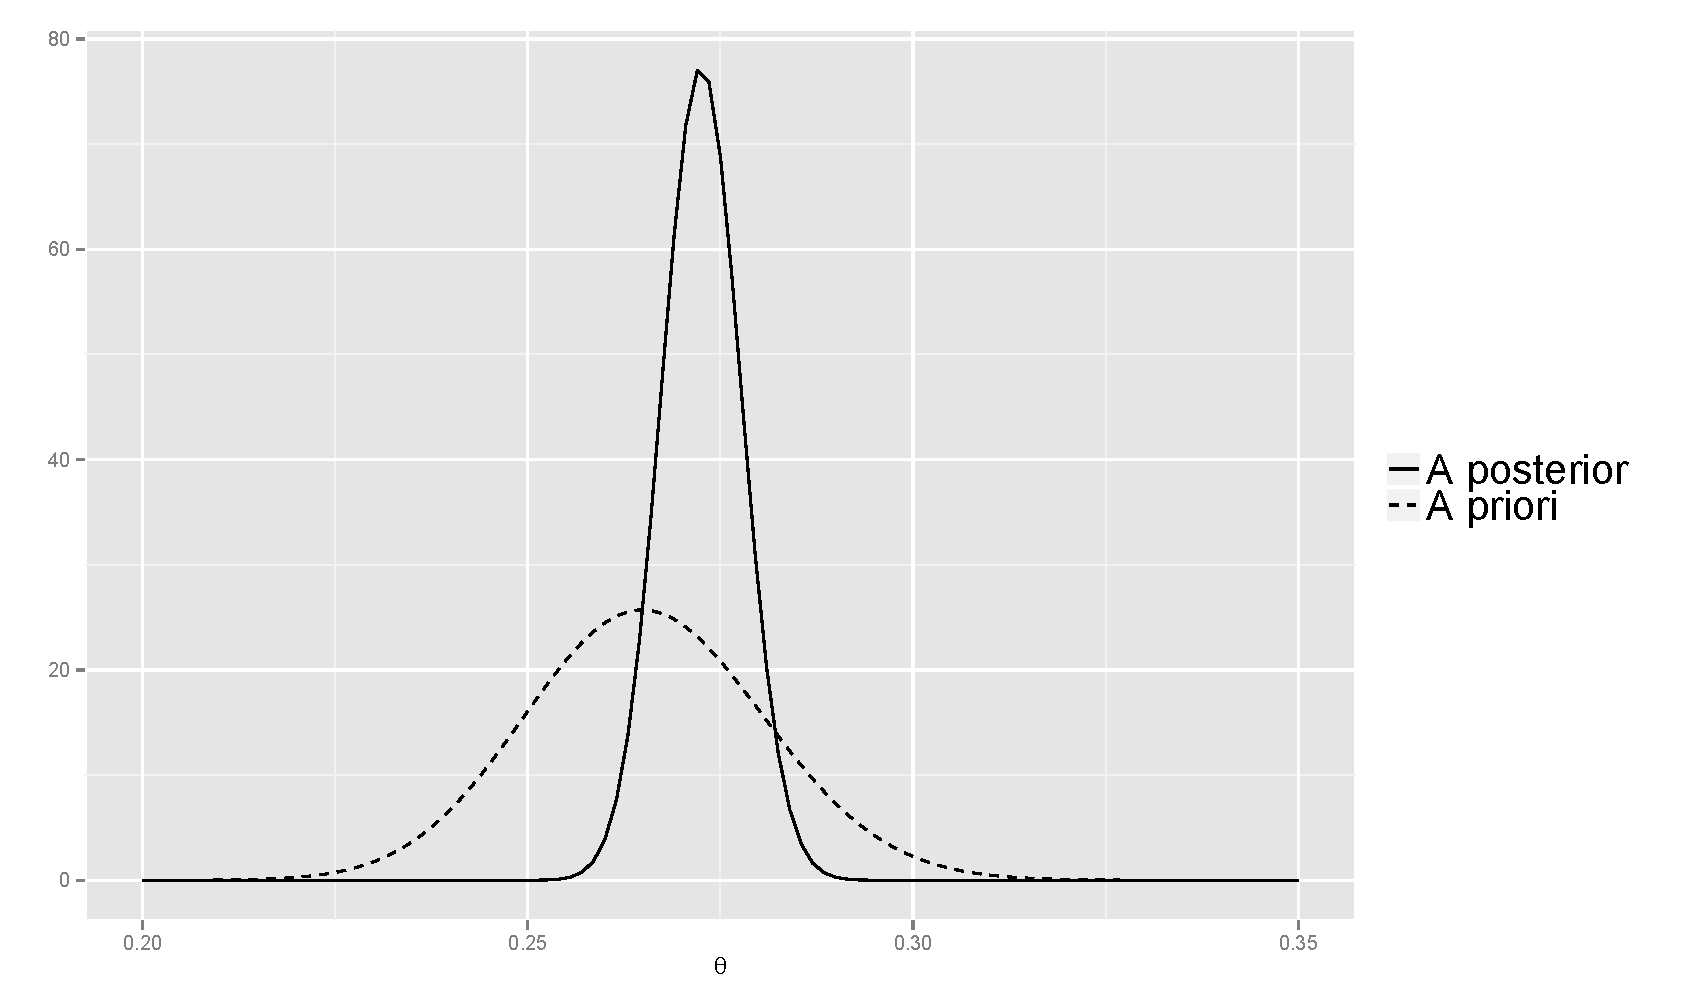
\includegraphics[scale=0.4]{BinomEj1.pdf}
    \caption{\emph{Funci\'on de densidad previa y funci\'on de densidad posterior para el ejemplo de bateo.}}
    \label{BinomEj1}
    \end{figure}
    
    Finalmente, notamos que los mismos resultados se encuentran cuando se analiza este conjunto de datos en \texttt{JAGS}, mediante el siguiente c\'odigo computacional.
    
\begin{knitrout}
\definecolor{shadecolor}{rgb}{0.933, 0.933, 0.933}\color{fgcolor}\begin{kframe}
\begin{alltt}
\hlstd{k} \hlkwb{<-} \hlkwd{nrow}\hlstd{(EfronMorris)}

\hlstd{Bin.model} \hlkwb{<-} \hlkwa{function}\hlstd{()\{}
\hlkwa{for}\hlstd{(i} \hlkwa{in} \hlnum{1} \hlopt{:} \hlstd{k)}
\hlstd{\{}
\hlstd{s[i]} \hlopt{~} \hlkwd{dbin}\hlstd{(theta, n[i])}
\hlstd{\}}
\hlstd{theta} \hlopt{~} \hlkwd{dbeta}\hlstd{(}\hlnum{215}\hlstd{,} \hlnum{595}\hlstd{)}
\hlstd{\}}

\hlstd{s} \hlkwb{<-} \hlkwd{round}\hlstd{(EfronMorris}\hlopt{$}\hlstd{n}\hlopt{*}\hlstd{EfronMorris}\hlopt{$}\hlstd{p)}
\hlstd{n} \hlkwb{<-} \hlstd{EfronMorris}\hlopt{$}\hlstd{n}

\hlstd{Bin.data} \hlkwb{<-} \hlkwd{list}\hlstd{(}\hlstr{"s"}\hlstd{,}\hlstr{"n"}\hlstd{,}\hlstr{"k"}\hlstd{)}
\hlstd{Bin.param} \hlkwb{<-} \hlkwd{c}\hlstd{(}\hlstr{"theta"}\hlstd{)}
\hlstd{Bin.inits} \hlkwb{<-} \hlkwa{function}\hlstd{()\{}
\hlkwd{list}\hlstd{(}\hlstr{"theta"}\hlstd{=}\hlkwd{c}\hlstd{(}\hlnum{0.5}\hlstd{))}
\hlstd{\}}

\hlstd{Bin.fit} \hlkwb{<-} \hlkwd{jags}\hlstd{(}\hlkwc{data}\hlstd{=Bin.data,} \hlkwc{inits}\hlstd{=Bin.inits, Bin.param,} \hlkwc{n.iter}\hlstd{=}\hlnum{10000}\hlstd{,}
                \hlkwc{n.burnin}\hlstd{=}\hlnum{1000}\hlstd{,} \hlkwc{model.file}\hlstd{=Bin.model)}

\hlkwd{print}\hlstd{(Bin.fit)}
\end{alltt}
\end{kframe}
\end{knitrout}

Al ejecutar los anteriore comandos, se encuentran que la estimaci\'on bayesiana posterior del par\'ametro $\theta$ est\'a dada por 0.274, mientras que el intervalo de credibilidad al 95\% es $(0.264,\ 0.284)$.
    
    Es posible analizar este conjunto de datos desde otra perspectiva al suponer que los jugadores no constituyen una muestra aleatoria y cada uno de ellos tiene un promedio de bateo diferente. Sin embargo, este an\'alisis se deja como ejercicio en un cap\'itulo posterior.
    \end{Eje}
    
    \begin{Eje}
    Continuando con el conjunto de datos de Efron y Morris, suponga que el entrenador de un equipo de las ligas inferiores est\'a interesado en adquirir los servicios de Max Alvis. Este jugador no tuvo un buen promedio de bateo en la temporada (est\'a situada en el \'ultimo lugar) y no tuvo muchos turnos al bate (solo 70 turnos en el resto de la temporada). El entrenador quiere conocer cu\'al ser\'a el n\'umero m\'as probable de hits que anotar\'a en la siguiente temporada. Teniendo en cuenta que es un jugador que viene de la liga profesional, lo m\'as conveniente es que tenga muchos turnos al bate, digamos 400.
    
    Para resolver este cuestionamiento, es conveniente recurrir a la funci\'on predictiva posterior, dada en el resultado \ref{ResPredBinom}. Para este an\'alisis, se define la caracterizaci\'on estructural de la distribuci\'on previa del jugador que est\'a dada por una $Beta(\alpha=7, \beta=38)$ (puesto que en la temporada del 1970, obtuvo 7 \emph{hits} de 45 turnos). La siguiente funci\'on en \texttt{R} permite obtener la distribuci\'on predictiva para este jugador, que se muestra en la figura \ref{PredBinom}.
    
\begin{knitrout}
\definecolor{shadecolor}{rgb}{0.933, 0.933, 0.933}\color{fgcolor}\begin{kframe}
\begin{alltt}
\hlstd{n} \hlkwb{<-} \hlnum{70}
\hlstd{s}\hlkwb{<-} \hlnum{14}
\hlstd{alp} \hlkwb{<-}\hlnum{7}
\hlstd{bet} \hlkwb{<-} \hlnum{38}
\hlstd{n.ast} \hlkwb{<-} \hlnum{400}

\hlstd{predictiva} \hlkwb{<-} \hlkwd{rep}\hlstd{(}\hlnum{NA}\hlstd{, n.ast}\hlopt{+}\hlnum{1}\hlstd{)}
\hlkwa{for}\hlstd{(k} \hlkwa{in} \hlnum{0}\hlopt{:}\hlstd{n.ast)}
\hlstd{\{}
\hlstd{predictiva[(k}\hlopt{+}\hlnum{1}\hlstd{)]} \hlkwb{<-}
  \hlkwd{choose}\hlstd{(n.ast, k)} \hlopt{*} \hlkwd{beta}\hlstd{(k}\hlopt{+}\hlstd{s}\hlopt{+}\hlstd{alp, bet}\hlopt{-}\hlstd{k}\hlopt{-}\hlstd{s}\hlopt{+}\hlstd{n.ast}\hlopt{+}\hlstd{n)} \hlopt{/} \hlkwd{beta}\hlstd{(s}\hlopt{+}\hlstd{alp, bet}\hlopt{-}\hlstd{s}\hlopt{+}\hlstd{n)}
\hlstd{\}}
\end{alltt}
\end{kframe}
\end{knitrout}
    
    \begin{figure}[!h]
    \centering
    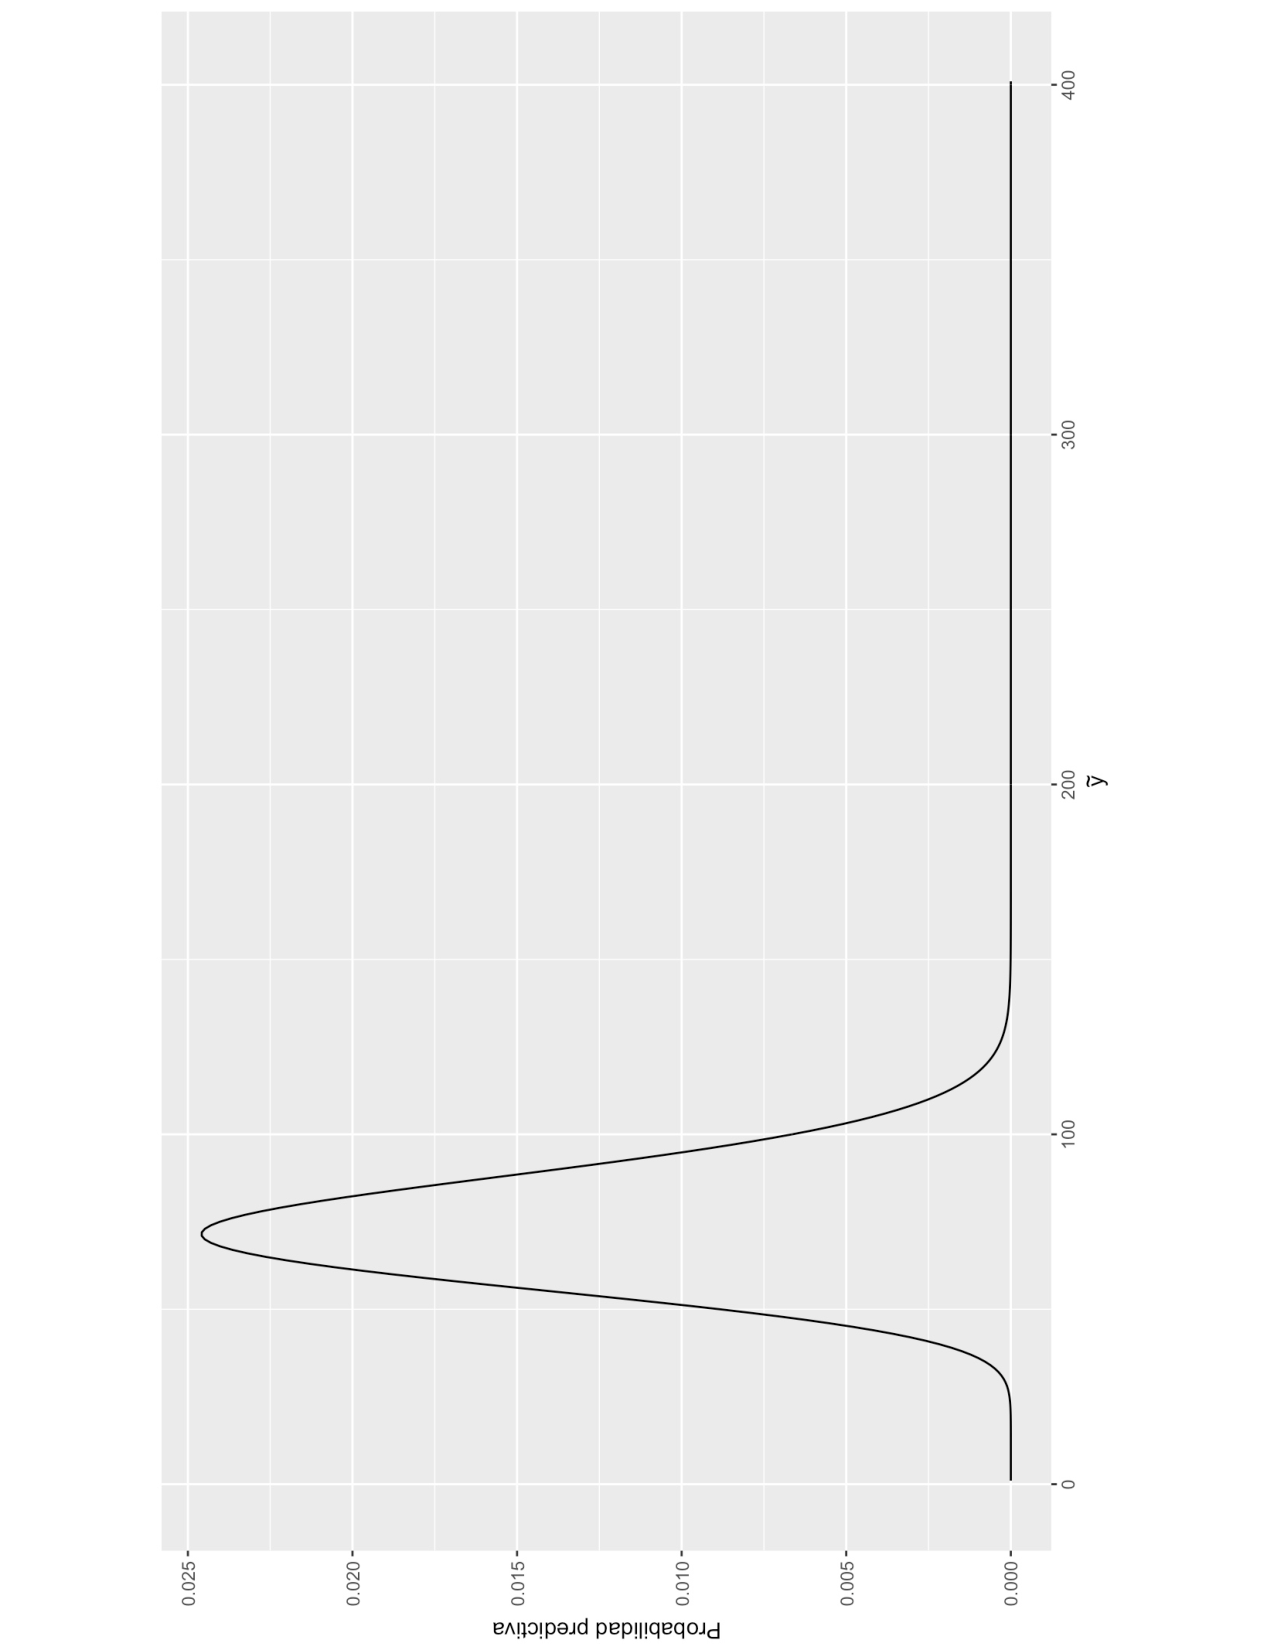
\includegraphics[scale=0.5,angle =-90 ]{predbinomial.pdf}
    \caption{\emph{Funci\'on de densidad predictiva posterior para el jugador Max Alvis.}}
    \label{PredBinom}
    \end{figure}
    
En la gr\'afica de la distribuci\'on predictiva posteiror, se observa que esta distribuci\'on se encuentra concentrado principalmenten en valores inferiores al 100 (el cual representa un porcentaje de \emph{hits} del 0.25). Adicionalmente, examinando los valores num\'ericos se puede encontrar que lo m\'as probable es que el jugador realice 71 hits en 400 turnos al bate, cifra que no convence al entrenador para adquirir los servicios del jugador.
    \end{Eje}
    
    \section{Modelo Binomial negativa}
    
    La distribuci\'on binomial negativa describe el n\'umero de ensayos necesarios para alcanzar un n\'umero determinado y fijo de \'exitos $k$ en una secuencia independiente de experimentos tipo Bernoulli. \'esta distribuci\'on es particularmente \'util cuando el porcentaje $\theta$ que se quiere estimar es muy peque\~no, como la proporci\'on de una poblaci\'on que padece de alguna enfermedad. La raz\'on por la que no se utiliza la distribuci\'on binomial es que al fijar el n\'umero de ensayos $n$, como el porcentaje $\theta$ es muy peque\~no, es muy probable que en en la muestra de tama\~no $n$ no se encuetre ning\'un paciente con la enfermedad; mientras que al utilizar la distribuci\'on binomial negativa, de antemano se garantiza que se obtendr\'a $k$ pacientes con la enfermedad en la muestra.
    
    Suponga que $Y$ es una variable aleatoria cuya distribuci\'on es Binomial negativa que representa el n\'umero de ensayos necesarios $y$ para alcanzar un n\'umero determinado y fijo de \'exitos $k$ en un experimento. La forma funcional de esta distribuci\'on es la siguiente
    \begin{equation}
    p(Y \mid \theta)=\binom{y-1}{k-1}\theta^k(1-\theta)^{y-k}I_{\{k,k+1,\ldots,\}}(y),
    \end{equation}
    
    As\'i como en la distribuci\'on Bernoulli y Binomial, el par\'ametro $\theta$ est\'a restringido al espacio $\Theta=[0,1]$. Luego, es admisible proponer que $\theta$ siga una distribuci\'on Beta. Por tanto, la distribuci\'on previa del par\'ametro $\theta$ est\'a dada por la expresi\'on (\ref{beta_distribution}). Bajo este marco de referencia se tienen los siguientes resultados
    
    \begin{Res}
    La distribuci\'on posterior del par\'ametro $\theta$ sigue una distribuci\'on
    \begin{equation*}
    \theta \mid Y \sim Beta(\alpha+k,\beta+y-k)
    \end{equation*}
    \end{Res}
    
    \begin{proof}
    \begin{align*}
    p(\theta \mid Y)&\propto p(Y \mid \theta)p(\theta \mid \alpha,\beta)\\
    &\propto \theta^{\alpha+k-1} (1-\theta)^{y+\beta-k-1}I_{[0,1]}(\theta)
    \end{align*}
    Por lo tanto, factorizando convenientemente, se llega a una expresi\'on id\'entica a la funci\'on de distribuci\'on de una variable aleatoria con distribuci\'on $Beta(\alpha+k,\beta+y-k)$.
    \end{proof}
    
    En algunas situaciones se puede encontrar una muestra de variables con distribuci\'on binomial negativa, por ejemplo, la entrevista de pacientes para encontrar cierta enfermedad puede llevarse a cabo en diferentes puntos de atenci\'on m\'edica o en diferentes ciudades del pa\'is. As\'i en cada punto de atenci\'on, se tendr\'a el dato correspondiente a una variable con distribuci\'on binomial negativa. El procedimiento inferencial bayesiano para estas situaciones se describe a continuaci\'on:
    
    \begin{Res}
    Cuando se tiene una sucesi\'on de variables aleatorias $Y_1,\ldots, Y_n$ independientes y con distribuci\'on $BinomialNegativa(k_i,\theta)$ $(i=1,\ldots,n)$, entonces la distribuci\'on posterior del par\'ametro de inter\'es es
    \begin{equation}
    \theta \mid Y_1,\ldots, Y_n \sim Beta(\alpha+\sum_{i=1}^n k_i,\beta+\sum_{i=1}^n y_i-\sum_{i=1}^n k_i)
    \end{equation}
    \end{Res}
    
    \begin{proof}
    Se deja como ejercicio para el lector.
    \end{proof}
    
    \begin{Eje}
    Una franquicia de investigaci\'on farmac\'eutica ha desarrollado un nuevo tratamiento farmacol\'ogico sobre pacientes diab\'eticos que padezcan, a su vez, de enfermedades card\'iacas, mejor conocidas como cardiopat\'ias, entre las que se pueden encontrar la angina de pecho, infarto de miocardio,  insuficiencia mitral, estenosis mitral, entre otras. Para evaluar el nuevo tratamiento, es necesario seleccionar una muestra, mediante el dise\~no de un experimento cl\'inico, de pacientes que tienen estas caracter\'isticas.
    
    Por otro lado, se sabe que la proporci\'on de personas que padecen de diabetes y que adem\'as tienen alg\'un tipo de condici\'on cardiaca es muy baja y es necesario obtener una estimaci\'on precisa de la proporci\'on de personas con estas condiciones. Con base en lo anteriormente expuesto, se puede pensar en seleccionar una grande de personas y utilizar un acercamiento binomial para estimar esta proporci\'on. Sin embargo, dado que la prevalencia de esta condici\'on es bastante baja, es posible que el n\'umero de personas en la muestra que presenten estas enfermedades sea nulo; por consiguiente, la estimaci\'on binomial no ser\'a, de ninguna forma, precisa.
    
    Por lo tanto, el dise\~no cl\'inico est\'a supeditado al uso de la distribuci\'on Binomial Negativa, en donde se entrevistar\'an pacientes, de una base de datos de un hospital de la ciudad asociado con la franquicia, hasta conseguir una muestra de cinco pacientes que padezcan de estas condiciones. Despu\'es de varios meses de entrevistas, se encontr\'o el quinto paciente en la entrevista n\'umero 1106.
    
    Mediante el an\'alisis bayesiano, suponiendo una distribuci\'on previa $Beta(0.5, 0.5)$, se llega a que la distribuci\'on posterior del par\'ametrtos $\theta$ es $Beta(0.5+5, 0.5+1106-5)=Beta(5.5, 1101.5)$. Por lo tanto, la estimaci\'on puntual del par\'ametro de inter\'es, que corresponde a la media de la distribuci\'on posterior, es 0.0049, que equivale una proporci\'on de 0.49\% de personas con estas enfermedades. El siguiente c\'odigo computacional muestra c\'omo se puede llegar a las mismas conclusiones con \verb'JAGS'
    
\begin{knitrout}
\definecolor{shadecolor}{rgb}{0.933, 0.933, 0.933}\color{fgcolor}\begin{kframe}
\begin{alltt}
\hlstd{BinNeg.model} \hlkwb{<-} \hlkwa{function}\hlstd{()\{}
\hlstd{y} \hlopt{~} \hlkwd{dnegbin}\hlstd{(theta,}\hlnum{5}\hlstd{)}
\hlstd{theta}\hlopt{~}\hlkwd{dbeta}\hlstd{(}\hlnum{0.5}\hlstd{,} \hlnum{0.5}\hlstd{)}
\hlstd{\}}

\hlcom{#BinNeg.data <- }
\hlcom{#list(y =1106)}
\hlstd{BinNeg.param} \hlkwb{<-} \hlkwd{c}\hlstd{(}\hlstr{"theta"}\hlstd{)}
\hlstd{BinNeg.inits} \hlkwb{<-} \hlkwa{function}\hlstd{()\{}
\hlkwd{list}\hlstd{(}\hlstr{"theta"}\hlstd{=}\hlnum{0.5}\hlstd{)}
\hlstd{\}}

\hlstd{BinNeg.fit} \hlkwb{<-} \hlkwd{jags}\hlstd{(}\hlkwc{data}\hlstd{=}\hlkwd{list}\hlstd{(}\hlkwc{y}\hlstd{=}\hlnum{1106}\hlstd{),} \hlkwc{inits}\hlstd{=BinNeg.inits, BinNeg.param,}
                   \hlkwc{n.iter}\hlstd{=}\hlnum{10000}\hlstd{,} \hlkwc{n.burn}\hlstd{=}\hlnum{1000}\hlstd{,} \hlkwc{model.file}\hlstd{=BinNeg.model)}

\hlkwd{print}\hlstd{(BinNeg.fit)}
\end{alltt}
\end{kframe}
\end{knitrout}
    
    Despu\'es de cinco mil iteraciones, la salida del anterior c\'odigo muestra la estimaci\'on puntual dada por 0.005 y un intervalo de credibilidad al 95\%, dado por $(0.002, 0.01)$.
    \end{Eje}
    
    \begin{Eje}\label{Eje1.3.2}
    Continuando con la tem\'atica del ejemplo anterior, suponga que la franquicia llev\'o a cabo la misma investigaci\'on en las 31 ciudades con mayor densidad poblacional de pa\'is. Como en la mayor\'ia de los casos, debido al condicionamiento presupuestal, el experimento difiri\'o en el n\'umero de \'exitos en cada caso. En total, se tuvieron 29620 entrevistas para un total de \'exitos de 152, tal como se muestra a continuaci\'on.
    
    \begin{center}
    \begin{verbatim}
    Ciudad                 y          k
    
    BOGOTA               1001         4
    MEDELLIN             978          6
    CALI                 999          5
    BARRANQUILLA         860          4
    CARTAGENA            1155         4
    CUCUTA               585          6
    BUCARAMANGA          1030         3
    IBAGUE               960          5
    SOLEDAD              1002         6
    SANTA MARTA          763          7
    SOACHA               1036         5
    PASTO                779          5
    MONTERIA             1158         4
    VILLAVICENCIO        1017         5
    BELLO                888          6
    MANIZALES            977          4
    VALLEDUPAR           1256         6
    BUENAVENTURA         1349         6
    NEIVA                1047         5
    PALMIRA              1088         5
    ARMENIA              649          3
    POPAYAN              765          4
    FLORIDABLANCA        699          5
    SINCELEJO            1042         4
    ITAGUI               1212         5
    BARRANCABERMEJA      660          5
    TULUA                671          5
    ENVIGADO             835          6
    DOSQUEBRADAS         997          5
    RIOHACHA             1146         4
    SINCELEJO            1016         5 
    \end{verbatim}
    \end{center}
    
    Mediante el an\'alisis bayesiano, suponiendo una distribuci\'on previa\footnote{N\'otese que es posible tambi\'en asignar una previa informativa $Beta(5.5, 1101.5)$, que da cuenta de la informaci\'on del estudio del ejemplo anterior.} no informativa $Beta(0.5, 0.5)$, se llega a que la distribuci\'on posterior del par\'ametrtos $\theta$ es $Beta(0.5+152, 0.5+29620-152)=Beta(152.5, 29468.5)$. Por lo tanto, la estimaci\'on puntual del par\'ametro de inter\'es, que corresponde a la media de la distribuci\'on posterior, es 0.0051, que equivale una proporci\'on de 0.51\% de personas con estas enfermedades. El siguiente c\'odigo computacional muestra c\'omo se puede llegar a las mismas conclusiones con JAGS
    
\begin{knitrout}
\definecolor{shadecolor}{rgb}{0.933, 0.933, 0.933}\color{fgcolor}\begin{kframe}
\begin{alltt}
\hlstd{BinNeg2.model} \hlkwb{<-} \hlkwa{function}\hlstd{()\{}
\hlkwa{for}\hlstd{(i} \hlkwa{in} \hlnum{1}\hlopt{:}\hlnum{31}\hlstd{)\{}
\hlstd{y[i]}\hlopt{~}\hlkwd{dnegbin}\hlstd{(theta,k[i])}
\hlstd{\}}
\hlstd{theta} \hlopt{~} \hlkwd{dbeta}\hlstd{(}\hlnum{0.5}\hlstd{,} \hlnum{0.5}\hlstd{)}
\hlstd{\}}

\hlstd{y} \hlkwb{<-} \hlkwd{c}\hlstd{(}\hlnum{1001}\hlstd{,} \hlnum{978}\hlstd{,} \hlnum{999}\hlstd{,} \hlnum{860}\hlstd{,} \hlnum{1155}\hlstd{,} \hlnum{585}\hlstd{,} \hlnum{1030}\hlstd{,} \hlnum{960}\hlstd{,} \hlnum{1002}\hlstd{,} \hlnum{763}\hlstd{,} \hlnum{1036}\hlstd{,} \hlnum{779}\hlstd{,} \hlnum{1158}\hlstd{,} \hlnum{1017}\hlstd{,}
       \hlnum{888}\hlstd{,} \hlnum{977}\hlstd{,} \hlnum{1256}\hlstd{,} \hlnum{1349}\hlstd{,} \hlnum{1047}\hlstd{,} \hlnum{1088}\hlstd{,} \hlnum{649}\hlstd{,} \hlnum{765}\hlstd{,} \hlnum{699}\hlstd{,} \hlnum{1042}\hlstd{,} \hlnum{1212}\hlstd{,} \hlnum{660}\hlstd{,} \hlnum{671}\hlstd{,} \hlnum{835}\hlstd{,} \hlnum{997}\hlstd{,} \hlnum{1146}\hlstd{,} \hlnum{1016}\hlstd{)}
\hlstd{k} \hlkwb{<-} \hlkwd{c}\hlstd{(}\hlnum{4}\hlstd{,} \hlnum{6}\hlstd{,} \hlnum{5}\hlstd{,} \hlnum{4}\hlstd{,} \hlnum{4}\hlstd{,} \hlnum{6}\hlstd{,} \hlnum{3}\hlstd{,} \hlnum{5}\hlstd{,} \hlnum{6}\hlstd{,} \hlnum{7}\hlstd{,} \hlnum{5}\hlstd{,} \hlnum{5}\hlstd{,} \hlnum{4}\hlstd{,} \hlnum{5}\hlstd{,} \hlnum{6}\hlstd{,} \hlnum{4}\hlstd{,} \hlnum{6}\hlstd{,} \hlnum{6}\hlstd{,} \hlnum{5}\hlstd{,} \hlnum{5}\hlstd{,} \hlnum{3}\hlstd{,} \hlnum{4}\hlstd{,} \hlnum{5}\hlstd{,} \hlnum{4}\hlstd{,}
       \hlnum{5}\hlstd{,} \hlnum{5}\hlstd{,} \hlnum{5}\hlstd{,} \hlnum{6}\hlstd{,} \hlnum{5}\hlstd{,} \hlnum{4}\hlstd{,} \hlnum{5}\hlstd{)}

\hlstd{BinNeg2.data} \hlkwb{<-} \hlkwd{list}\hlstd{(}\hlstr{"y"}\hlstd{,} \hlstr{"k"}\hlstd{)}
\hlstd{BinNeg2.param} \hlkwb{<-} \hlkwd{c}\hlstd{(}\hlstr{"theta"}\hlstd{)}
\hlstd{BinNeg2.inits} \hlkwb{<-} \hlkwa{function}\hlstd{()\{}
\hlkwd{list}\hlstd{(}\hlstr{"theta"}\hlstd{=}\hlnum{0.5}\hlstd{)}
\hlstd{\}}
\hlstd{BinNeg2.fit} \hlkwb{<-} \hlkwd{jags}\hlstd{(}\hlkwc{data}\hlstd{=BinNeg2.data,} \hlkwc{inits}\hlstd{=BinNeg2.inits, BinNeg2.param,} \hlkwc{n.iter}\hlstd{=}\hlnum{10000}\hlstd{,} \hlkwc{n.burnin}\hlstd{=}\hlnum{1000}\hlstd{,} \hlkwc{model.file}\hlstd{=BinNeg2.model)}

\hlkwd{print}\hlstd{(BinNeg2.fit)}
\end{alltt}
\end{kframe}
\end{knitrout}
    
    Despu\'es de cinco mil iteraciones, la salida del anterior c\'odigo muestra la estimaci\'on puntual dada por 0.005 y un intervalo de credibilidad al 95\%, dado por $(0.004, 0.006)$, mucho m\'as estrecho que el intervalo de credibilidad del anterior ejercicio.
    \end{Eje}
    
    Una vez observados los datos actuales y encontrada la distribuci\'on posterior, se puede encontrar la distribuci\'on predictiva posterior de una nueva variable con distribuci\'on binomial negativa. Es decir, se puede definir el mecanismo probabil\'istico para el n\'umero de ensayos necesarios para encontrar $\tilde{k}$ \'exitos.
    \begin{Res}
    Despu\'es de la recolecci\'on de datos, la distribuci\'on predictiva posterior para una nueva variable $\tilde{Y}$ est\'a dada por
    \begin{equation*}
    p(\tilde{Y}|Y_1,\cdots,Y_n)=\binom{\tilde{y}-1}{\tilde{k}-1}\frac{Beta(\alpha+\tilde{k}+\sum k_i,\beta+\tilde{y}-\tilde{k}+\sum y_i-\sum k_i)}{Beta(\alpha+\sum k_i,\beta+\sum y_i-\sum k_i)}I_{\{\tilde{k},\tilde{k}+1,\cdots\}}(\tilde{y})
    \end{equation*}
    \end{Res}
    
    \begin{proof}
    \begin{align*}
    &\ \ \ p(\tilde{Y}|Y_1,\cdots,Y_n)\\
    &=\int p(\tilde{Y}|\theta)p(\theta|Y_1,\cdots,Y_n)d\theta\\
    &=\int_{0}^1\binom{\tilde{y}-1}{\tilde{k}-1}\theta^{\alpha+\tilde{k}}(1-\theta)^{\beta+\tilde{y}-\tilde{k}}I_{\{\tilde{k},\tilde{k}+1,\cdots\}}(\tilde{y})\frac{\theta^{\sum k_i-1}(1-\theta)^{\sum y_i-\sum k_i-1}}{Beta(\alpha+\sum k_i,\beta+\sum y_i-\sum k_i)}d\theta\\
    &=\binom{\tilde{y}-1}{\tilde{k}-1}\frac{I_{\{\tilde{k},\tilde{k}+1,\cdots\}}(\tilde{y})}{Beta(\alpha+\sum k_i,\beta+\sum y_i-\sum k_i)}\int_{0}^1\theta^{\alpha+\tilde{k}+\sum k_i-1}(1-\theta)^{\beta+\tilde{y}-\tilde{k}+\sum y_i-\sum k_i-1}d\theta\\
    &=\binom{\tilde{y}-1}{\tilde{k}-1}\frac{Beta(\alpha+\tilde{k}+\sum k_i,\beta+\tilde{y}-\tilde{k}+\sum y_i-\sum k_i)}{Beta(\alpha+\sum k_i,\beta+\sum y_i-\sum k_i)}I_{\{\tilde{k},\tilde{k}+1,\cdots\}}(\tilde{y})
    \end{align*}
    \end{proof}
    
    \begin{Eje}
    Siguiendo con los datos del Ejemplo \ref{Eje1.3.2}, suponga que se quiere recolectar informaci\'on de 3 pacientes con cardiopat\'ia en cierta ciudad, y se quiere conocer acerca del n\'umero de entrevistas necesarias. Utilizando la distribuci\'on previa $Beta(0.5,0.5)$ y los datos de las 31 ciudades del ejemplo, se tiene que la distribuci\'on predictiva para el n\'umero de entrevistas necesarias para encontrar 3 pacientes est\'a dada por
    \begin{align*}
    &\ \ \ \ p(\tilde{Y}|Y_1,\cdots,Y_n)\\
    &=\binom{\tilde{y}-1}{4}\frac{Beta(0.5+5+152,0.5+\tilde{y}-5+29620-152)}{Beta(0.5+152,0.5+29620-152)}I_{\{5,6,\cdots\}}(\tilde{y})\\
    &=\binom{\tilde{y}-1}{4}\frac{Beta(157.5,\tilde{y}+29463.5)}{Beta(152.5,29468.5)}I_{\{5,6,\cdots\}}(\tilde{y})
    \end{align*}
    
    Con los siguientes c\'odigos se puede calcular la anterior funci\'on predictiva.
    
\begin{knitrout}
\definecolor{shadecolor}{rgb}{0.933, 0.933, 0.933}\color{fgcolor}\begin{kframe}
\begin{alltt}
\hlstd{predict}\hlkwb{<-}\hlkwa{function}\hlstd{(}\hlkwc{y}\hlstd{,}\hlkwc{alfa}\hlstd{,}\hlkwc{beta}\hlstd{,}\hlkwc{s}\hlstd{,}\hlkwc{n}\hlstd{,}\hlkwc{k}\hlstd{)\{}
  \hlkwd{choose}\hlstd{(y}\hlopt{-}\hlnum{1}\hlstd{, k}\hlopt{-}\hlnum{1}\hlstd{)} \hlopt{*} \hlkwd{exp}\hlstd{(}\hlkwd{lbeta}\hlstd{(alfa}\hlopt{+}\hlstd{k}\hlopt{+}\hlstd{s, beta}\hlopt{+}\hlstd{y}\hlopt{-}\hlstd{k}\hlopt{+}\hlstd{n}\hlopt{-}\hlstd{s)} \hlopt{-} \hlkwd{lbeta}\hlstd{(alfa}\hlopt{+}\hlstd{s, beta}\hlopt{+}\hlstd{n}\hlopt{-}\hlstd{s))}
\hlstd{\}}

\hlstd{alfa} \hlkwb{<-} \hlstd{beta} \hlkwb{<-} \hlnum{0.5}
\hlstd{s} \hlkwb{<-} \hlnum{152}\hlstd{; n} \hlkwb{<-} \hlnum{29620}\hlstd{; k} \hlkwb{<-} \hlnum{5}
\hlstd{fun} \hlkwb{<-} \hlkwd{rep}\hlstd{(}\hlnum{NA}\hlstd{)}
\hlkwa{for}\hlstd{(y} \hlkwa{in} \hlnum{5}\hlopt{:}\hlnum{5000}\hlstd{)\{}
   \hlstd{fun[y}\hlopt{-}\hlnum{4}\hlstd{]} \hlkwb{<-} \hlkwd{predict}\hlstd{(y, alfa, beta, s, n, k)}
\hlstd{\}}
\hlkwd{sum}\hlstd{(fun)}
\end{alltt}
\begin{verbatim}
## [1] 1
\end{verbatim}
\end{kframe}
\end{knitrout}
    
    \begin{figure}[!htb]\label{jefber}
    \centering
    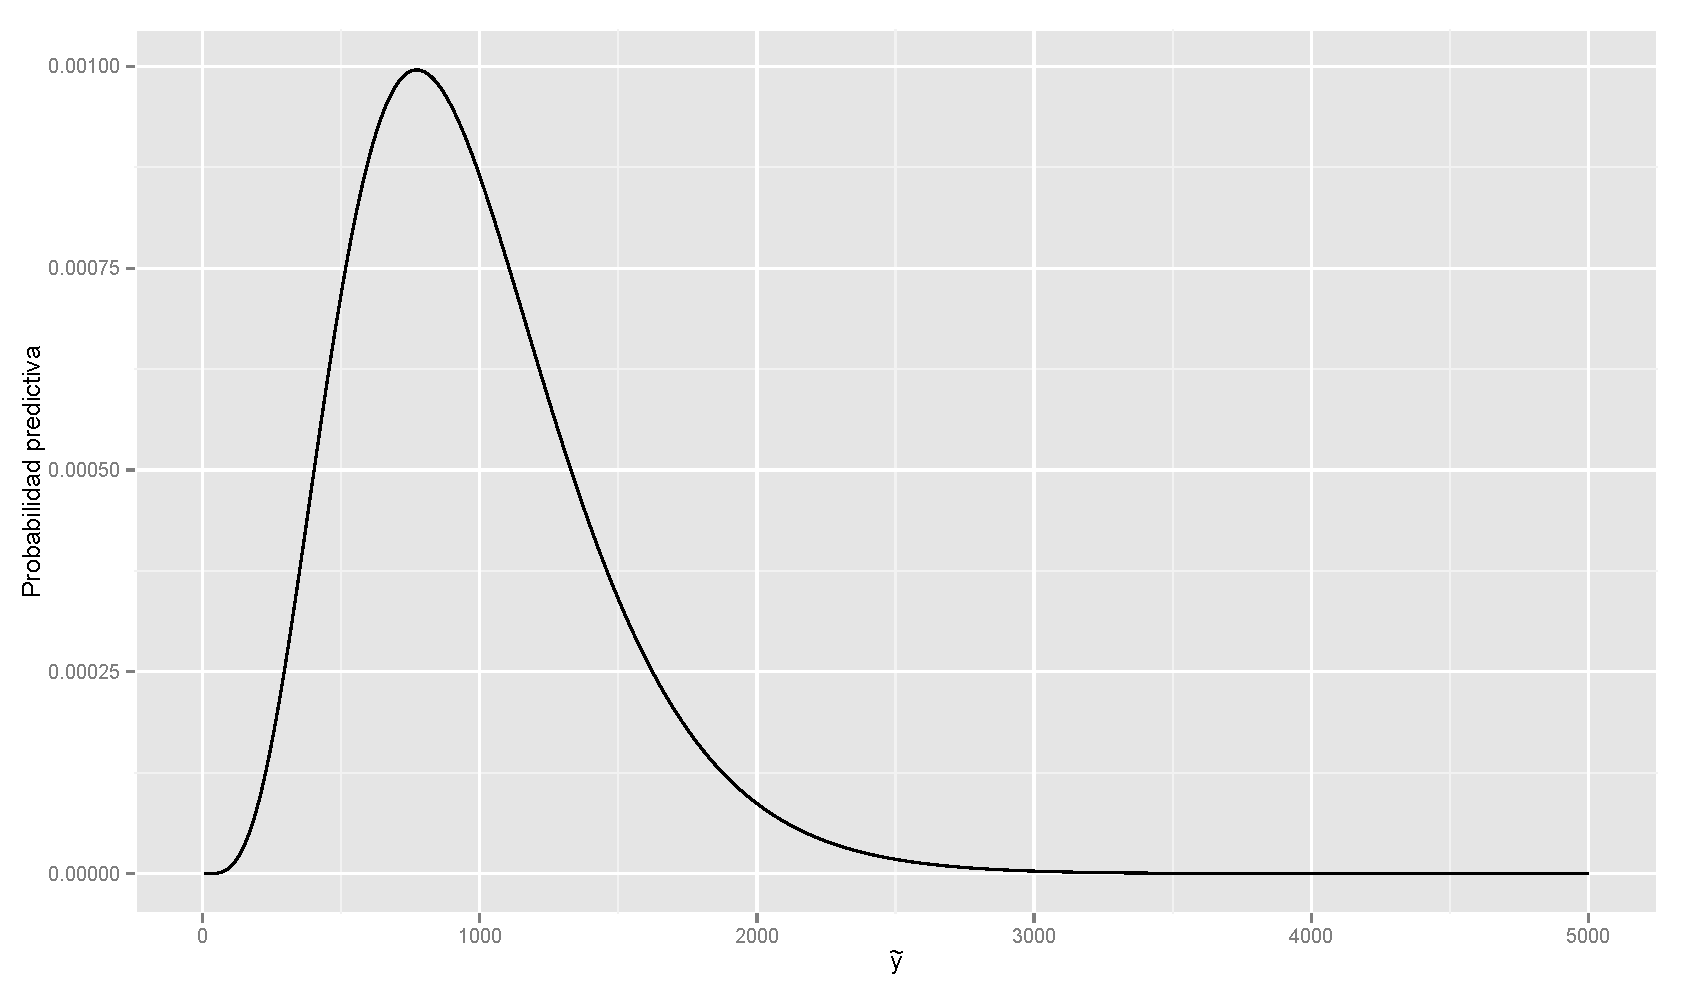
\includegraphics[scale=0.35]{pred_negabinom.pdf}
    \caption{\emph{Distribuci\'on predictiva posterior para el n\'umero de entrevistas necesarias para encontrar 5 pacientes usando los datos del ejemplo 2.3.2}.}
    \end{figure}
    
    Se puede ver que el n\'umero de entrevistas que tiene mayor probabilidad asociadas es el valor 772, usando el comando
\begin{knitrout}
\definecolor{shadecolor}{rgb}{0.933, 0.933, 0.933}\color{fgcolor}\begin{kframe}
\begin{alltt}
\hlkwd{which}\hlstd{(fun}\hlopt{==}\hlkwd{max}\hlstd{(fun))}\hlopt{+}\hlnum{4}
\end{alltt}
\begin{verbatim}
## [1] 772
\end{verbatim}
\end{kframe}
\end{knitrout}
    Tambi\'en, se puede calcular la probabilidad de que en menos de 500 entrevistas se encuentren los 5 pacientes es de solo el 12\% usando el comando
\begin{knitrout}
\definecolor{shadecolor}{rgb}{0.933, 0.933, 0.933}\color{fgcolor}\begin{kframe}
\begin{alltt}
\hlkwd{sum}\hlstd{(fun[}\hlnum{1}\hlopt{:}\hlstd{(}\hlnum{500}\hlopt{-}\hlnum{4}\hlstd{)])}
\end{alltt}
\begin{verbatim}
## [1] 0.1201
\end{verbatim}
\end{kframe}
\end{knitrout}
    \end{Eje}
    
    \section{Modelo Poisson}
    
    Suponga que $\mathbf{Y}=\{Y_1,\ldots,Y_n\}$ es una muestra aleatoria de variables con distribuci\'on Poisson con par\'ametro $\theta$, la funci\'on de distribuci\'on conjunta o la funci\'on de verosimilitud est\'a dada por
    \begin{align*}
    p(\mathbf{Y} \mid \theta)&=\prod_{i=1}^n\frac{e^{-\theta}\theta^{y_i}}{y_i!}I_{\{0,1,\ldots\}}(y_i)\\
    &=\frac{e^{-n\theta}\theta^{\sum_{i=1}^ny_i}}{\prod_{i=1}^ny_i!}I_{\{0,1,\ldots\}^n}(y_1,\ldots,y_n)
    \end{align*}
    
    donde $\{0,1\ldots\}^n$ denota el producto cartesiano $n$ veces sobre el conjunto $\{0,1\ldots\}$. Por otro lado, como el par\'ametro $\theta$ est\'a restringido al espacio $\Theta=(0,\infty)$, entonces es posible formular varias opciones para la distribuci\'on previa del par\'ametro. Algunas opciones se encuentran considerando la distribuci\'on exponencial o la distribuci\'on chi-cuadrado o la distribuci\'on Gamma. N\'otese que las dos primeras distribuciones son casos particulares de la \'ultima. Por lo tanto, la distribuci\'on previa del par\'ametro $\theta$ est\'a dada por
    \begin{equation}\label{prior_Gamma}
    p(\theta \mid \alpha,\beta)=\frac{\beta^\alpha}{\Gamma(\alpha)}\theta^{\alpha-1} e^{-\beta\theta}I_{(0,\infty)}(\theta).
    \end{equation}
    
    Bajo este marco de referencia se tienen el siguiente resultado con respecto a la distribucion posterior del par\'ametro de inter\'es $\theta$.
    \begin{Res}
    \label{ResPoissonPost}
    La distribuci\'on posterior del par\'ametro $\theta$ est\'a dada por
    \begin{equation*}
    \theta \mid \mathbf{Y} \sim Gamma\left(\sum_{i=1}^ny_i+\alpha,n+\beta\right)
    \end{equation*}
    \end{Res}
    
    \begin{proof}
    \begin{align*}
    p(\theta \mid \mathbf{Y})&\propto p(\mathbf{Y} \mid \theta)p(\theta \mid \alpha,\beta)\\
    &=\frac{I_{\{0,1,\ldots\}^n}(y_1,\ldots,y_n)}{\prod_{i=1}^ny_i!}\frac{\beta^\alpha}{\Gamma(\alpha)}
    \theta^{\alpha-1}\theta^{\sum_{i=1}^ny_i}e^{-\beta\theta}e^{-n\theta}I_{(0,\infty)}(\theta)\\
    &\propto \theta^{\sum_{i=1}^ny_i+\alpha-1}e^{-(\beta+n)\theta}I_{(0,\infty)}(\theta)
    \end{align*}
    Por lo tanto, factorizando convenientemente, se encuentra una expresi\'on id\'entica a la funci\'on de distribuci\'on de una variable aleatoria con distribuci\'on $Gamma(\sum_{i=1}^ny_i+\alpha,n+\beta)$.
    \end{proof}
    
    Utilizando el resultado anterior, se tiene que la estimaci\'on Bayesiana del par\'ametro $\theta$ est\'a dada por
    \begin{equation*}
    \hat{\theta}=\frac{\sum_{i=1}^ny_i+\alpha}{n+\beta}.
    \end{equation*}
    
    La anterior expresi\'on sugiere tomar los par\'ametros de la distribuci\'on previa $\alpha$ y $\beta$ de la siguiente manera: $\beta$ representa el n\'umero de observaciones en la informaci\'on previa, mientras que $\alpha$ representa la suma de los datos de la informaci\'on previa. De esta forma, $\alpha/\beta$ representa la estimaci\'on previa del par\'ametro $\theta$. Y la estimaci\'on Bayesiana de $\theta$ se puede escribir como
    \begin{align*}
    \hat{\theta}&=\frac{\sum_{i=1}^ny_i+\alpha}{\beta+n}\\
    &=\frac{n}{n+\beta}*\frac{\sum y_i}{n}+\frac{\beta}{n+\beta}*\frac{\alpha}{\beta}\\
    &=\frac{n}{n+\beta}*\hat{\theta_C}+\frac{\beta}{n+\beta}*\hat{\theta_P}\\
    \end{align*}
    Es decir, la estimaci\'on Bayesiana de $\theta$ es un promedio ponderado entre la estimaci\'on cl\'asica y la estimaci\'on previa del par\'ametro $\theta$, donde los pesos dependen directamente del tama\~no muestral de la informaci\'on actual y de la informaci\'on previa. 
    
    A continuaci\'on estudiamos las distribuciones predictivas previa y posterior de una nueva observaci\'on 
    \begin{Res}\label{Res1.4.2}
    La distribuci\'on predictiva previa para una observaci\'on $\mathbf{y}=\{y_1,\ldots,y_n\}$ de la muestra aleatoria est\'a dada por
    \begin{equation}\label{Pre_prior_Poisson}
    p(\mathbf{Y})=\frac{\Gamma(\sum_{i=1}^ny_i+\alpha)}{\Gamma(\alpha)}\frac{\beta^\alpha}{(n+\beta)^{\sum_{i=1}^ny_i+\alpha}}
    \frac{I_{\{0,1,\ldots\}^n}(y_1,\ldots,y_n)}{\prod_{i=1}^ny_i!}
    \end{equation}
    y define una aut\'entica funci\'on de densidad de probabilidad continua.
    \end{Res}
    
    \begin{proof}
    De la definici\'on de funci\'on de distribuci\'on predictiva se tiene que 
    \begin{align*}
    p(\mathbf{Y})&=\int p(\mathbf{Y} \mid \theta)p(\theta \mid \alpha,\beta)\ d\theta\\
    &=\int_0^{\infty} \frac{e^{-n\theta}\theta^{\sum_{i=1}^ny_i}}{\prod_{i=1}^ny_i!}I_{\{0,1,\ldots\}^n}(y_1,\ldots,y_n)
    \frac{\beta^\alpha \theta^{\alpha-1} e^{-\beta\theta}}{\Gamma(\alpha)}\ d\theta\\
    &=\frac{\Gamma(\sum_{i=1}^ny_i+\alpha)}{\Gamma(\alpha)}\frac{\beta^\alpha}{(n+\beta)^{\sum_{i=1}^ny_i+\alpha}}
    \frac{I_{\{0,1,\ldots\}^n}(y_1,\ldots,y_n)}{\prod_{i=1}^ny_i!}\\
    &\hspace{2cm}\times
    \int_0^{\infty} \frac{(n+\beta)^{\sum_{i=1}^ny_i+\alpha}}{\Gamma(\sum_{i=1}^ny_i+\alpha)}
    \theta^{\sum_{i=1}^ny_i+\alpha-1}e^{-(\beta+n)\theta} \ d\theta\\
    &=\frac{\Gamma(\sum_{i=1}^ny_i+\alpha)}{\Gamma(\alpha)}\frac{\beta^\alpha}{(n+\beta)^{\sum_{i=1}^ny_i+\alpha}}
    \frac{I_{\{0,1,\ldots\}^n}(y_1,\ldots,y_n)}{\prod_{i=1}^ny_i!}
    \end{align*}
    \end{proof}
    
    En el caso en que la muestra aleatoria estuviera constituida por una sola variable aleatoria, entonces $n=1$ y si, en particular, los hiper-par\'ametros de la distribuci\'on previa fuesen $\alpha=\beta=1$, entonces no es dif\'icil ver, utilizando la definici\'on de la funci\'on matem\'atica Gamma, que la funci\'on de distribuci\'on predictiva (\ref{Pre_prior_Poisson}) estar\'ia dada por
    \begin{align}\label{Pre_prior_poisson1}
    p(Y)&=\frac{\Gamma(y+1)}{\Gamma(1)}\frac{1}{2^{y+1}}\frac{I_{\{0,1,\ldots\}}(y)}{y!} \notag\\
    &=\frac{1}{2^{y+1}}I_{\{0,1,\ldots\}}(y)
    \end{align}
    
    Para chequear la convergencia de la anterior distribuci\'on es necesario recurrir a los resultados del an\'alisis matem\'atico \cite[p. 361]{Apostol}. Dado que el espacio de muestreo de la variable aleatoria $Y$ es $\{0,1,\ldots\}$, entonces la suma infinita converge a uno lo que conlleva a que, en este caso particular, $P(Y)$ sea una aut\'entica funci\'on de densidad de probabilidad.
    \begin{align*}
    \sum_{y=0}^{\infty}p(Y=y)=\sum_{y=0}^{\infty}\left(\frac{1}{2}\right)^{y+1}=\frac{1}{2}\sum_{y=0}^{\infty}\left(\frac{1}{2}\right)^{y}
    =\frac{1}{2}\frac{1}{1-1/2}=1
    \end{align*}
    
    y podemos afirmar que la expresion (\ref{Pre_prior_poisson1}) s\'i representa una funci\'on de densidad de una variable discreta. Ahora, consideramos la distribuci\'on predictiva poseterior de una muestra aleatoria, esta distribuci\'on se presenta en el siguiente resultado.
    
    \begin{Res}
    \label{ResPoissonPred}
    Despu\'es de la recolecci\'on de los datos, la distribuci\'on predictiva posterior para una nueva posible observaci\'on $\tilde{\mathbf{y}}=\{\tilde{y}_1,\ldots,\tilde{y}_{n^*}\}$, de tama\~no $n^*$, est\'a dada por
    
    \begin{align}
    p(\tilde{\mathbf{y}} \mid \mathbf{Y})&=\frac{\Gamma(\sum_{i=1}^{n^*}\tilde{y}_i+\sum_{i=1}^ny_i+\alpha)}{\Gamma(\sum_{i=1}^ny_i+\alpha)}
    \frac{(\beta+n)^{\sum_{i=1}^ny_i+\alpha}}{({n^*}+\beta+n)^{\sum_{i=1}^{n^*}\tilde{y}_i+\sum_{i=1}^ny_i+\alpha}}\notag\\
    &\hspace{5cm}\times
    \frac{I_{\{0,1,\ldots\}^{n^*}}(\tilde{y}_1,\ldots,\tilde{y}_{n^*})}{\prod_{i=1}^{n^*}\tilde{y}_i!}
    \end{align}
    \end{Res}
    
    \begin{proof}
    De la definici\'on de funci\'on de distribuci\'on predictiva, y haciendo uso del mismo razonamiento en la demostraci\'on del Resultado \ref{Res1.4.2}, se tiene la prueba inmediata.
    \end{proof}
    
    La anterior distribuci\'on corresponde a una distribucion multivariada que nos permite calcular probabilidades predictivas para cualesquieras valores de $\tilde{y}_1$, $\cdots$, $\tilde{y}_{n^*}$; sin embargo, en algunas situaciones, como por ejemplo, cuando $\theta$ representa el n\'umero promedio de alg\'un suceso en una regi\'on geogr\'afica, entonces al momento de la predicci\'on, podemos estar interesados en predecir el n\'umero total o el n\'umero promedio de sucesos en la nueva muestra aleatoria de regiones geogr\'aficos. Es decir, podemos estar m\'as interesados en la distribuci\'on de $\sum_{i=1}^{n^*} \tilde{y}_i$ o de $\sum_{i=1}^{n^*} \tilde{y}_i/n^*$ en vez de la distribuci\'on conjunta de $\tilde{y}_1$, $\cdots$, $\tilde{y}_{n^*}$. La distribuci\'on predictiva de $\sum_{i=1}^{n^*} \tilde{y}_i$ se presenta en el siguiente resultado, y con esta distribuci\'on se puede obtener f\'acilmente probabilidades predictivas para $\sum_{i=1}^{n^*} \tilde{y}_i/n^*$.
    
    \begin{Res}
    Despu\'es de la recolecci\'on de los datos, la distribuci\'on predictiva posterior para la suma de un vector de observaciones nuevas $\left(\tilde{y}_1,\ldots,\tilde{y}_{n^*}\right)$, $\tilde{s} = \sum_{y=1}^{n^*} \tilde{y}_i$, est\'a dada por:
    
    \begin{align}\label{pre_pos_poisson_sum}
    p(\tilde{\mathbf{s}} \mid \mathbf{Y})&=\frac{\Gamma(\tilde{s}+\sum_{i=1}^ny_i+\alpha)}{\Gamma(\sum_{i=1}^ny_i+\alpha)}
    \frac{(n+\beta)^{\sum_{i=1}^ny_i+\alpha}}{({n^*}+n+\beta)^{\tilde{s}+\sum_{i=1}^ny_i+\alpha}}\frac{(n^*)^{\tilde{s}}I_{\{0,1,\ldots\}}(\tilde{s})}{\tilde{s}!}
    \end{align}
    \end{Res}
    
    \begin{proof}
    Usando el hecho de que $\theta|\mathbf{Y}\sim Gamma(\sum_{i=1}^{n}y_i+\alpha,n+\beta)$ y $\tilde{s}|\theta\sim Poisson(n^*\theta)$ se procede a calcular $\tilde{s}/p(\mathbf{y})$,
    as\'i:
    \begin{align*}
    &\ \ \ \ p(\tilde{s}|\mathbf{y}) \\
    &= \int_{\Omega} p(\tilde{s}|\theta)p(\theta|\mathbf{y})d\theta\\
    & = \int_{\Omega} \frac{(n^{*}\theta)^{\tilde{s}}e^{-n^*\theta}}{\tilde{s}!} I_{\{0,1,\ldots\}}(\tilde{s}) (\beta+n)^{\sum_{i=1}^{n}y_i+\alpha}\frac{\theta^{\tilde{s}+\sum_{i=1}^{n}y_i+\alpha-1}}{\Gamma(\sum_{i=1}^{n}y_i+\alpha)}e^{-(\beta+n)\theta}I_{(0,\infty)}(\theta) d\theta\\
    &= \frac{(n^*)^{\tilde{s}}(\beta+n)^{\sum_{i=1}^{n}y_i+\alpha}}{\tilde{s}!\Gamma(\sum_{i=1}^{n}y_i+\alpha)}I_{\{0,1,\ldots\}}(\tilde{s})\int_{0}^{\infty}\theta^{\sum_{i=1}^{n}y_i+\alpha-1}e^{-(n^*+\beta+n)\theta}d\theta
    \end{align*}
    
    Agrupando las constantes para obtener la integral de una distribuci\'on gamma con $\alpha=\tilde{s}+\sum_{i=1}^{n}y_i+\alpha$ y $\beta=n^*+n+\beta$ se obtiene el resultado.
    \end{proof}
    
    En la pr\'actica, evaluar directamente la expresi\'on (\ref{pre_pos_poisson_sum}) puede ocasionar problemas num\'ericas, por la presencia de la funci\'on Gamma y las potencias. Para evitar dicha dificultad, podemos usar la siguiente expresi\'on equivalente cuando $\tilde{s}=1,2,\cdots$: 
    \begin{equation*}
    p(\tilde{\mathbf{s}} \mid \mathbf{Y})=\frac{\Gamma(\tilde{s})}{B(\tilde{s},\sum_{i=1}^ny_i+\alpha)}
    \left(\frac{n+\beta}{n^*+n+\beta}\right)^{\sum_{i=1}^ny_i+\alpha}\frac{(n^*)^{\tilde{s}}}{(n^*+n+\beta)^{\tilde{s}}\tilde{s}!}
    \end{equation*}
    
    Cuando $\tilde{s}=0$, la distribuci\'on predictiva es simplemente:
    
    \begin{equation*}
    p(\tilde{\mathbf{s}} \mid \mathbf{Y})=
    \left(\frac{n+\beta}{n^*+n+\beta}\right)^{\sum_{i=1}^ny_i+\alpha}
    \end{equation*}
    
    Ahora, debido a la complejidad de la expresi\'on en (\ref{pre_pos_poisson_sum}), es pr\'acticamente imposible comprobar anal\'iticamente $\sum_{i=0}^\infty p(\tilde{s}=i)=1$, y tambi\'en muy dif\'icil encontrar una expresi\'on matem\'atica cerrada de la esperanza de la variable $\mathbf{\tilde{s}}$, sin embargo, en situaciones pr\'acticas, se puede usar aproximaciones num\'ericas tal como se ver\'a en el ejemplo al final de esta secci\'on.
    
    En el ejemplo \ref{EjemPoisson} se consider\'o la situaci\'on cuando no se tiene ninguna informaci\'on previa, la distribuci\'on previa que se debe usar est\'a dada por
    \begin{equation*}
    p(\theta)\propto\theta^{-1/2},
    \end{equation*}
    
    que corresponde a una distribuci\'on previa impropia, puesto que $\int_{0}^\infty \theta^{-1/2}=\infty$. Sin embargo, este hecho no afecta que la inferencia posterior se pueda llevar a cabo, puesto que la distribuci\'on posterior est\'a dada por
    \begin{equation*}
    \theta|\mathbf{Y}\sim Gamma(\sum y_i+1/2,n)
    \end{equation*}
    y la estimaci\'on Bayesiana del par\'ametro $\theta$ viene dada por 
    \begin{equation*}
    \hat{\theta}=\frac{\sum y_i+1/2}{n}.
    \end{equation*}
    
    la cual es muy similar a la estimaci\'on cl\'asica de $\theta$ dada por $\bar{Y}$.
    
    Cuando se utiliza la distribuci\'on previa no informativa de Jeffreys, la distribuci\'on predictiva para nuevas observaciones $\tilde{y}={\tilde{y}_1,\cdots,\tilde{y}_{n^*}}$ y $\tilde{s}=\sum_{i=1}^{n^*}\tilde{y_i}$ est\'an dadas por
    \begin{equation}\label{pred_posson_Jeffreys}
    p(\tilde{\mathbf{y}} \mid \mathbf{Y})=\frac{\Gamma(\sum_{i=1}^{n^*}\tilde{y}_i+\sum_{i=1}^ny_i+0.5)}{\Gamma(\sum_{i=1}^ny_i+0.5)}
    \frac{n^{\sum_{i=1}^ny_i+0.5}}{({n^*}+n)^{\sum_{i=1}^n\tilde{y}_i+\sum_{i=1}^ny_i+0.5}}
    \frac{I_{\{0,1,\ldots\}^{n^*}}(\tilde{y}_1,\ldots,\tilde{y}_{n^*})}{\prod_{i=1}^{n^*}\tilde{y}_i!}
    \end{equation}
    
    y
    \begin{equation}\label{pred1_posson_Jeffreys}
    p(\tilde{\mathbf{s}} \mid \mathbf{Y})=\frac{\Gamma(\tilde{s}+\sum_{i=1}^ny_i+0.5)}{\Gamma(\sum_{i=1}^ny_i+0.5)}
    \frac{n^{\sum_{i=1}^ny_i+0.5}}{({n^*}+n)^{\tilde{s}+\sum_{i=1}^ny_i+0.5}}\frac{I_{\{0,1,\ldots\}}(\tilde{s})}{\tilde{s}!}
    \end{equation}
    
    \begin{Eje}\label{Datos_Poisson}
    Por pol\'iticas gubernamentales, los alcaldes las ciudades est\'an obligados a realizar un seguimiento exhaustivo al comportamiento de la accidentalidad en las v\'ias urbanas y medirlo en t\'erminos del n\'umero de accidentes de tr\'ansito. Lo anterior es necesario para evaluar la gesti\'on de las autoridades administrativas y evaluar las pol\'iticas p\'ublicas que el gobierno de la ciudad ha implementado para disminuir esta cifra.
    
    Suponga que la alcald\'ia de una ciudad quiere implementar una estrategia educativa para disminuir el n\'umero de accidentes de tr\'ansito, generados por manejar en estado de embriaguez. Para esto, se registraron durante diez d\'ias 30 d\'ias el n\'umero de accidentes de tr\'ansito por ebriedad del conductor. Los datos para cada uno de los d\'ias son 22, 9, 9, 20, 10, 14, 11, 14, 11, 11, 19, 12, 8, 9, 16, 8, 13, 8, 14, 12, 14, 11, 14, 13, 11, 14, 13, 11, 7, 12.
    
    Es posible modelar la variable aleatoria n\'umero de accidentes de tr\'ansito en un d\'ia mediante una distribuci\'on de Poisson puesto que el promedio muestral y la varianza muestral de los datos son semejantes. Para este conjunto de datos, el promedio equivale a 12.33, mientras que la varianza es de 12.51. El histograma de los valores observados se puede ver en la figura \ref{EjemPoisson1}.
    
    \begin{figure}[!h]
    \centering
    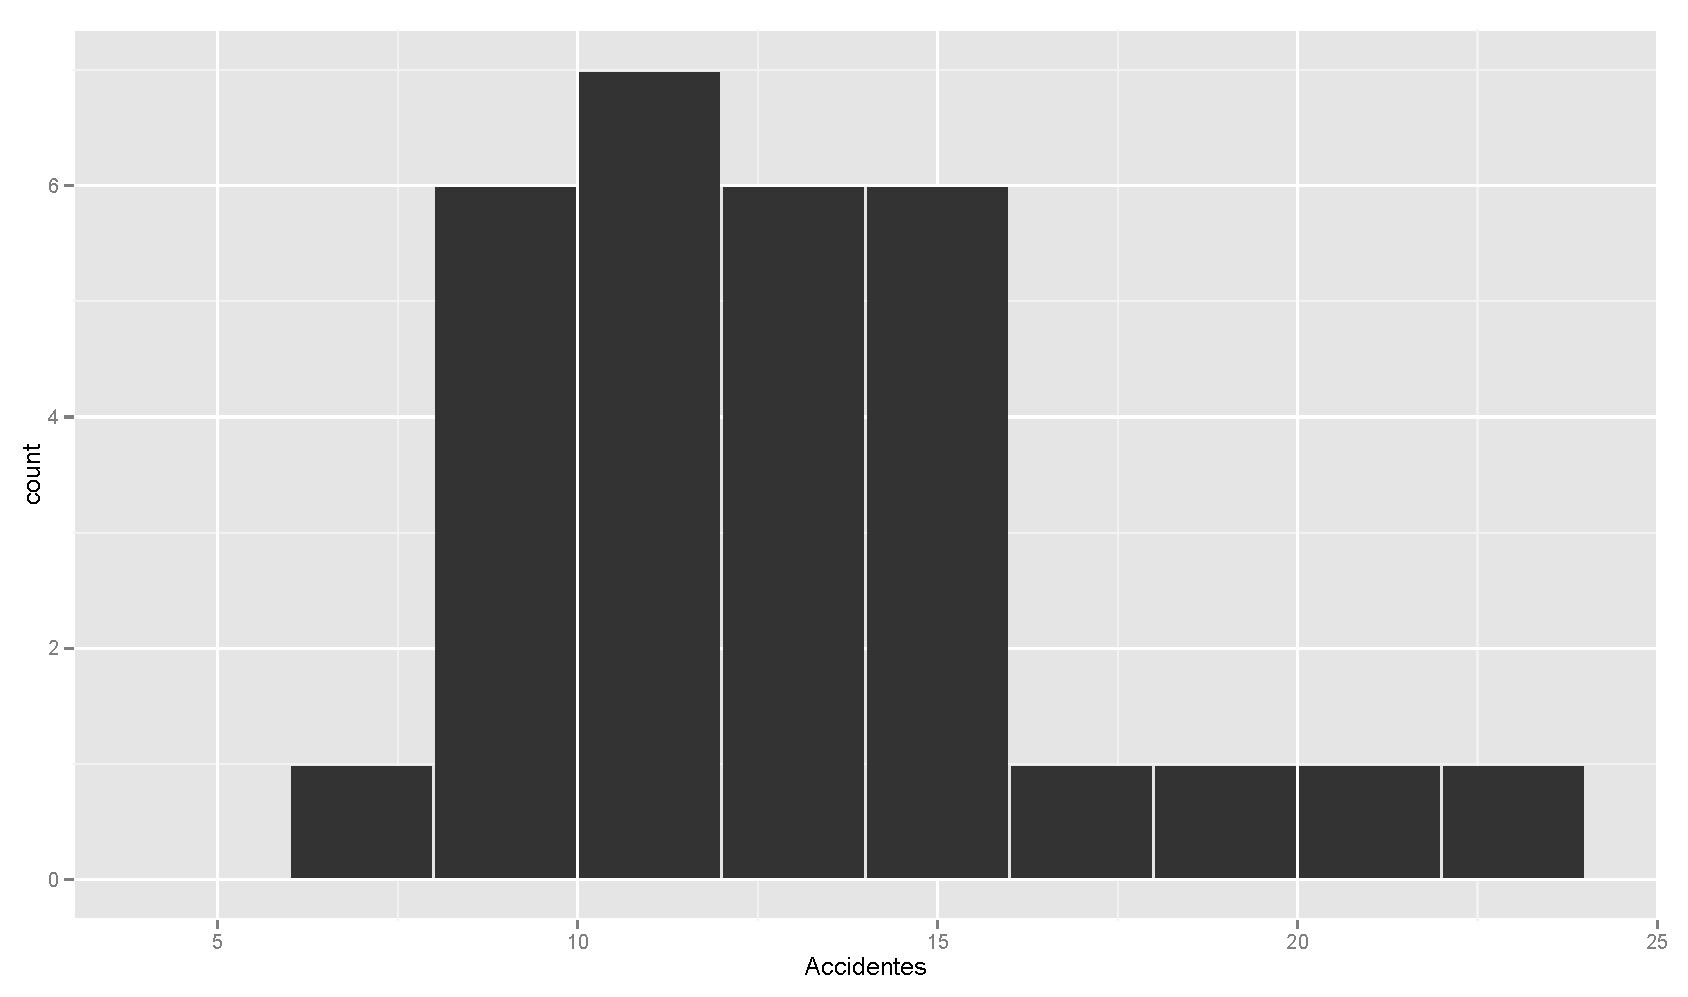
\includegraphics[scale=0.5]{EjemPoisson1.pdf}
    \caption{\emph{Histograma para los datos de accidentes de tr\'ansito.}}
    \label{EjemPoisson1}
    \end{figure}
    
    En primera instancia, es posible realizar un an\'alisis no informativo, al formular una distribuci\'on previa de Jeffreys, utilizando el resultado del ejemplo \ref{EjemPoisson1} de la p\'agina \pageref{EjemPoisson1}, que indica que una distribuci\'on previa no informativa es proporcional a $\theta^{-1/2}$, para lo cual la distribuci\'on posterior $Gamma(\sum_{i=1}^n y_i+1/2, n)$. De esta manera, la distribuci\'on posterior del par\'ametro de inter\'es es $Gamma(370.5, 30)$. Por lo tanto, un estimador de $\theta$ est\'a dado por la media de la distribuci\'on posterior que es $370.5/30=12.35$, muy cercano al valor del estimador de m\'axima verosimilitud correspondiente al promedio muestral. La figura \ref{EjemPoisson2} (lado izquierdo) muestra el comportamiento de las distribuciones de Jeffreys y posterior para este ejemplo.
    
    Por otro lado, bas\'andose en datos hist\'oricos, la alcald\'ia observ\'o que, en el mismo periodo del a\~no anterior, ocurrieron 37 accidentes en 9 d\'ias de observaci\'on. Luego, una distribuci\'on previa informativa\footnote{En la pr\'actica, se recomienda que los valores de los hiperpar\'ametros $\alpha$ y $\beta$ correspondan a la suma del n\'umero de eventos m\'as uno y n\'umero de observaciones, respectivamente.} est\'a dada por $Gamma(\alpha=38,\beta=9)$. Luego, apelando al resultado \ref{ResPoissonPost}, la distribuci\'on posterior corresponde a una $Gamma(370+38, 30+9)=Gamma(408, 39)$. Para este caso, un estimador de $\theta$ est\'a dado por la media de la distribuci\'on posterior que es $480/39=12.31$. La figura \ref{EjemPoisson2} (lado derecho) muestra el comportamiento de las distribuciones previa (informativa) y posterior para este ejemplo.
    
    \begin{figure}[!h]
    \centering
    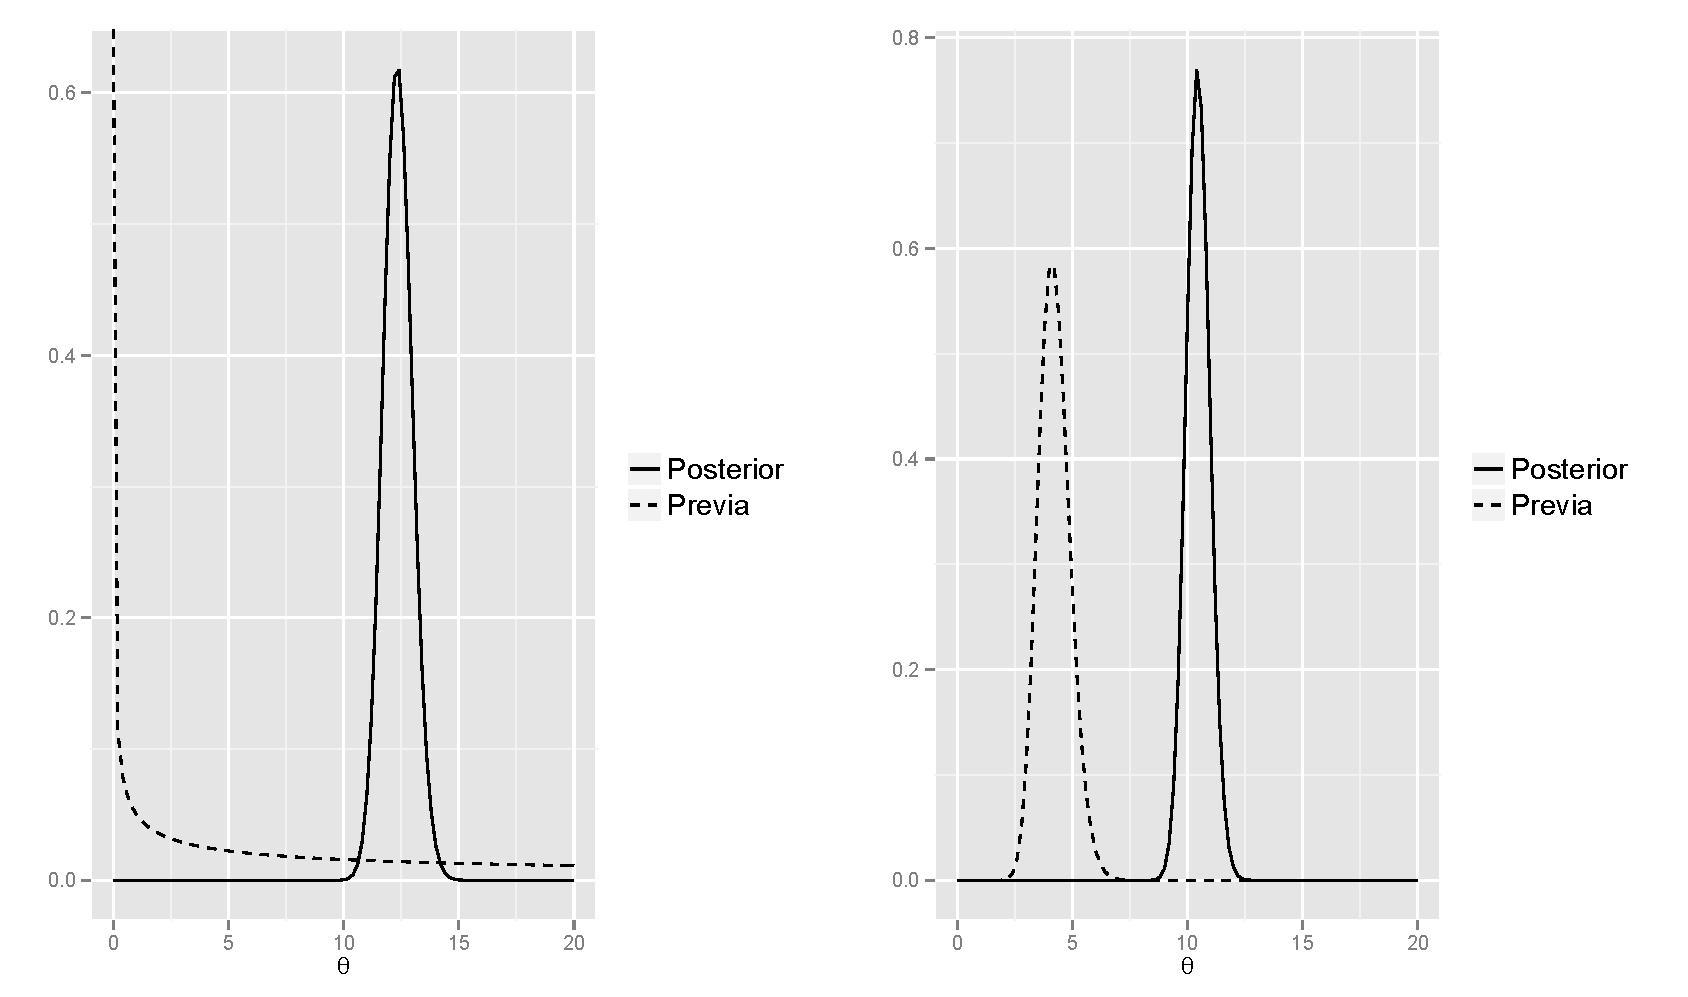
\includegraphics[width=18cm,height=8cm]{EjemPoisson2.pdf}
    \caption{\emph{Distribuci\'on previa y distribuci\'on posterior para el ejemplo del tr\'ansito con dos distribuciones previas diferentes (el lado izquierdo representa el caso cuando se usa la previa no informativa, el lado derecho la previa informativa).}}
    \label{EjemPoisson2}
    \end{figure}
    
    A continuaci\'on se examina la distribuci\'on predictiva. En la figura \ref{pred_post_pois} se grafica la distribuci\'on predictiva para una nueva observaci\'on cuando se usa la previa no informativa y la previa informativa. Los c\'odigos para el c\'alculo cuando se usa la previa no informativa es como siguen:
\begin{knitrout}
\definecolor{shadecolor}{rgb}{0.933, 0.933, 0.933}\color{fgcolor}\begin{kframe}
\begin{alltt}
\hlstd{Trans} \hlkwb{<-} \hlkwd{c}\hlstd{(}\hlnum{22}\hlstd{,} \hlnum{9}\hlstd{,} \hlnum{9}\hlstd{,} \hlnum{20}\hlstd{,} \hlnum{10}\hlstd{,} \hlnum{14}\hlstd{,} \hlnum{11}\hlstd{,} \hlnum{14}\hlstd{,} \hlnum{11}\hlstd{,} \hlnum{11}\hlstd{,} \hlnum{19}\hlstd{,} \hlnum{12}\hlstd{,} \hlnum{8}\hlstd{,} \hlnum{9}\hlstd{,} \hlnum{16}\hlstd{,} \hlnum{8}\hlstd{,} \hlnum{13}\hlstd{,} \hlnum{8}\hlstd{,} \hlnum{14}\hlstd{,} \hlnum{12}\hlstd{,}
\hlnum{14}\hlstd{,} \hlnum{11}\hlstd{,} \hlnum{14}\hlstd{,} \hlnum{13}\hlstd{,} \hlnum{11}\hlstd{,} \hlnum{14}\hlstd{,} \hlnum{13}\hlstd{,} \hlnum{11}\hlstd{,} \hlnum{7}\hlstd{,} \hlnum{12} \hlstd{)}
\hlstd{n} \hlkwb{<-} \hlkwd{length}\hlstd{(Trans)}
\hlstd{pre.Transito.NoInf} \hlkwb{<-} \hlkwa{function}\hlstd{(}\hlkwc{s}\hlstd{)\{}
\hlkwa{if}\hlstd{(s}\hlopt{>}\hlnum{0}\hlstd{)\{}
  \hlstd{val} \hlkwb{<-} \hlkwd{gamma}\hlstd{(s)}\hlopt{*}\hlstd{(n}\hlopt{/}\hlstd{(n}\hlopt{+}\hlnum{1}\hlstd{))}\hlopt{^}\hlstd{(}\hlkwd{sum}\hlstd{(Trans)}\hlopt{+}\hlnum{0.5}\hlstd{)}\hlopt{/}
      \hlstd{(}\hlkwd{beta}\hlstd{(s,}\hlkwd{sum}\hlstd{(Trans)}\hlopt{+}\hlnum{0.5}\hlstd{)}\hlopt{*}\hlkwd{prod}\hlstd{(}\hlnum{1}\hlopt{:}\hlstd{s)}\hlopt{*}\hlstd{(n}\hlopt{+}\hlnum{1}\hlstd{)}\hlopt{^}\hlstd{s)}
\hlstd{\}}
\hlkwa{if}\hlstd{(s}\hlopt{==}\hlnum{0}\hlstd{)\{}
 \hlstd{val} \hlkwb{<-} \hlstd{(n}\hlopt{/}\hlstd{(n}\hlopt{+}\hlnum{1}\hlstd{))}\hlopt{^}\hlstd{(}\hlkwd{sum}\hlstd{(Trans)}\hlopt{+}\hlnum{0.5}\hlstd{)}
\hlstd{\}}
\hlstd{val}
\hlstd{\}}
\hlstd{s.max} \hlkwb{<-} \hlnum{40}\hlstd{; s.val} \hlkwb{<-} \hlnum{0}\hlopt{:}\hlstd{s.max; pre.NoInf.val} \hlkwb{<-} \hlkwd{c}\hlstd{()}
\hlkwa{for}\hlstd{(i} \hlkwa{in} \hlnum{1}\hlopt{:}\hlkwd{length}\hlstd{(s.val))\{}
\hlstd{pre.NoInf.val[i]} \hlkwb{<-} \hlkwd{pre.Transito.NoInf}\hlstd{(s.val[i])}
\hlstd{\}}
\hlkwd{sum}\hlstd{(pre.NoInf.val)}
\end{alltt}
\begin{verbatim}
## [1] 1
\end{verbatim}
\end{kframe}
\end{knitrout}
    N\'otese que en los anteriores c\'odigos, se us\'o como valor m\'aximo de 40 para la variable $\mathbf{\tilde{s}}$ a pesar de que \'esta toma valores infinitos, pero al ver que la suma de las probabilidades desde el valor 0 hasta el m\'aximo de 40 es igual a 1, podemos concluir que la probabilidad de que $\mathbf{\tilde{s}}$ tome valores mayores a 40 es pr\'acticamente nula.
    
    Adicionalmente, podemos tener una aproximaci\'on de la esperanza de la variable $\mathbf{\tilde{s}}$ como
\begin{knitrout}
\definecolor{shadecolor}{rgb}{0.933, 0.933, 0.933}\color{fgcolor}\begin{kframe}
\begin{alltt}
\hlkwd{sum}\hlstd{(pre.NoInf.val}\hlopt{*}\hlstd{s.val)}
\end{alltt}
\begin{verbatim}
## [1] 12.35
\end{verbatim}
\end{kframe}
\end{knitrout}
    
    Finalmente, en la figura \ref{predic_Poisson} se observa la distribuci\'on predictiva posterior usando dos diferentes distribuciones previas. 
    
    \begin{figure}[!h]\label{predic_Poisson}
    \centering
    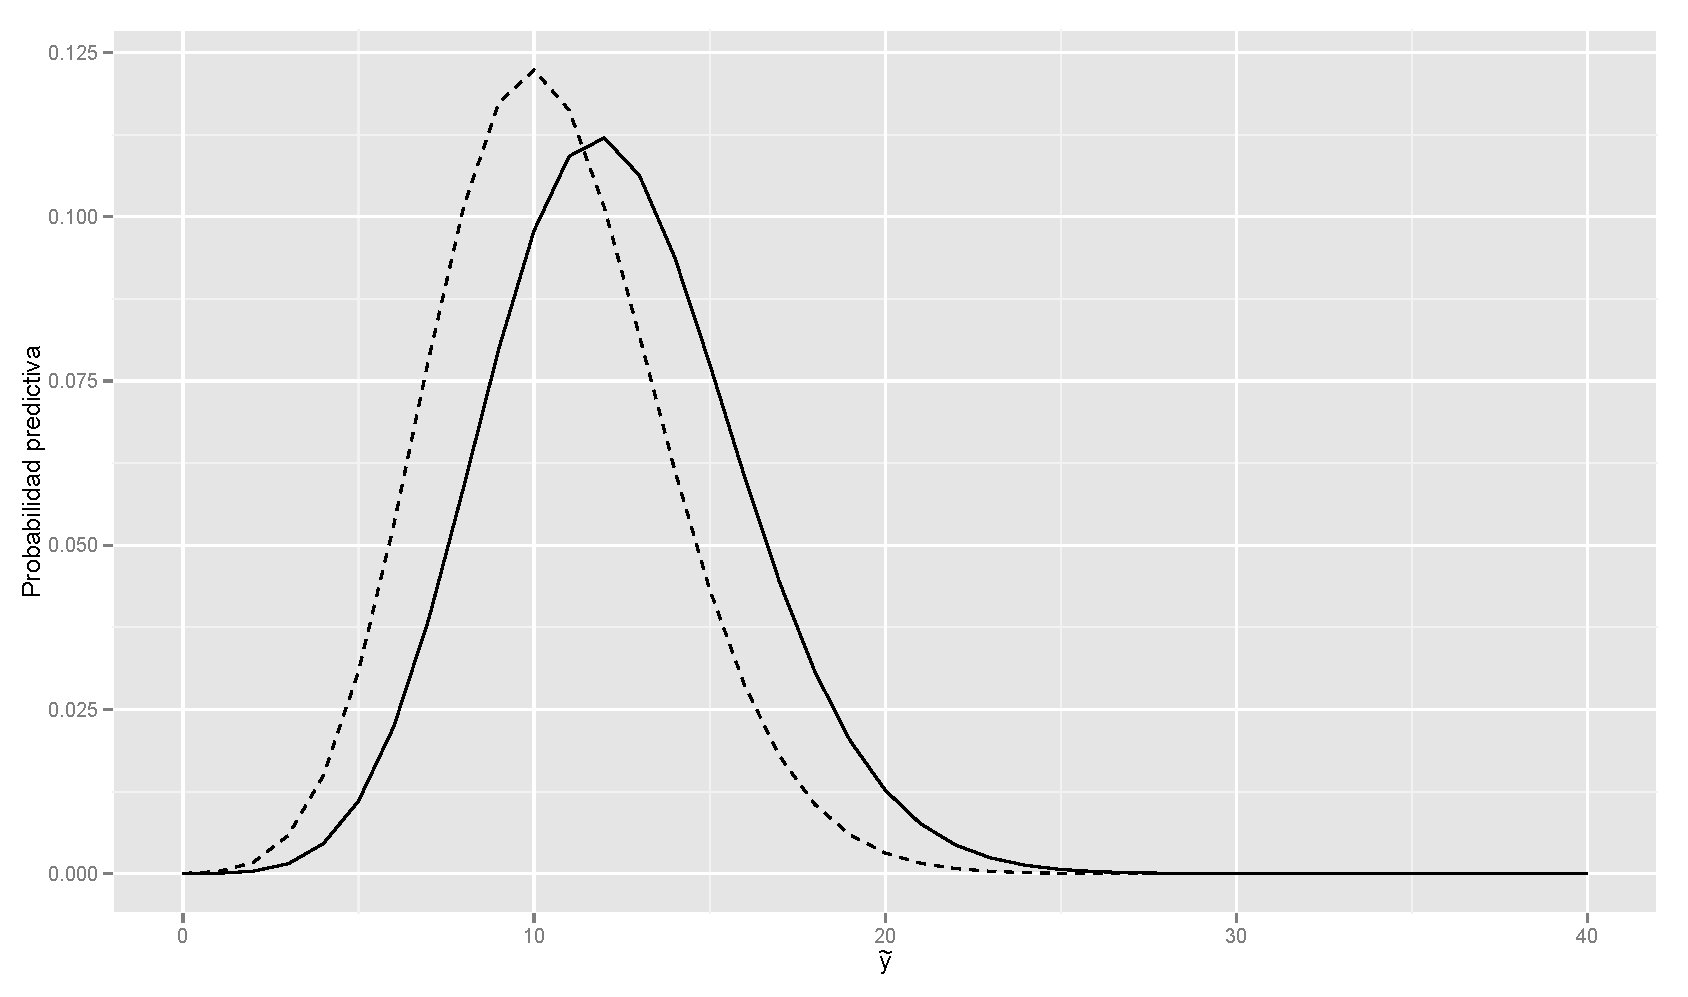
\includegraphics[scale=0.4]{predpostpois.pdf}
    \caption{\emph{Distribuci\'on predictiva posterior para $n*=1$ para el ejemplo del tr\'ansito. La l\'inea s\'olida denota la distribuci\'on predictiva obtenida con la previa no informativa, la l\'inea continua denota la obtenida con la previa $Gamma(\alpha=38,\beta=9)$.}}
    \label{pred_post_pois}
    \end{figure}
    
    \end{Eje}
    
    \section{Modelo exponencial}
    
    Suponga que $\mathbf{Y}=\{Y_1,\ldots,Y_n\}$ corresponde a una muestra de variables aleatorias con distribuci\'on Exponencial. Luego, la funci\'on de distribuci\'on conjunta o verosimilitud est\'a dada por
    
    \begin{align}
    p(\mathbf{Y} \mid \theta)&=\prod_{i=1}^n\theta e^{-\theta y}I_{(0,\infty)}(y_i) \notag \\
    &=\theta^n e^{-\theta \sum_{i=1}^ny_i}I_{(0,\infty)^n}(y_1,\ldots,y_n)
    \end{align}
    
    Donde $(0,\infty)^n$ denota el producto cartesiano $n$ veces sobre el intervalo $(0,\infty)$. Por otro lado, como el par\'ametro $\theta$ est\'a restringido al espacio $\Theta=(0,\infty)$, entonces es posible formular varias opciones para la distribuci\'on previa del par\'ametro, al igual que en la distribuci\'on Poisson. As\'i mismo, suponga que la distribuci\'on previa para el par\'ametro de inter\'es es la distribuci\'on Gamma tal como aparece en la expresi\'on (\ref{prior_Gamma}). Bajo este marco de referencia se tienen los siguientes resultados
    
    \begin{Res}
    La distribuci\'on posterior del par\'ametro $\theta$ sigue una distribuci\'on
    \begin{equation*}
    \theta \mid \mathbf{Y} \sim Gamma\left(\alpha+n,\beta+\sum_{i=1}^ny_i\right)
    \end{equation*}
    \end{Res}
    
    \begin{proof}
    \begin{align*}
    p(\theta \mid \mathbf{Y})&\propto p(\mathbf{Y} \mid \theta)p(\theta \mid \alpha,\beta)\\
    &=\theta^n e^{-\theta \sum_{i=1}^ny_i}I_{(0,\infty)^n}(y_1,\ldots,y_n)\frac{\beta^\alpha \theta^{\alpha-1} e^{-\beta\theta}}{\Gamma(\alpha)}I_{(0,\infty)}(\theta)\\
    &\propto \theta^{\alpha+n-1}e^{-(\beta+\sum_{i=1}^ny_i)}I_{(0,\infty)}(\theta)
    \end{align*}
    Por lo tanto, factorizando convenientemente, se encuentra una expresi\'on id\'entica a la funci\'on de distribuci\'on de una variable aleatoria con distribuci\'on $Gamma(\alpha+n,\beta+\sum_{i=1}^ny_i)$.
    \end{proof}
    
    \begin{Res}\label{predictiva_exponencial}
    La distribuci\'on predictiva previa para una observaci\'on $\mathbf{y}=\{y_1,\ldots,y_n\}$ de la muestra aleatoria est\'a dada por
    \begin{equation}\label{predictiva_exponencial_for}
    p(\mathbf{Y})=\frac{\Gamma(\alpha+n)}{\Gamma(\alpha)}\frac{\beta^\alpha}{(\beta+\sum_{i=1}^ny_i)^{\alpha+n}}
    I_{(0,\infty)^n}(y_1,\ldots,y_n)
    \end{equation}
    y define una aut\'entica funci\'on de densidad de probabilidad continua.
    \end{Res}
    
    \begin{proof}
    De la definici\'on de funci\'on de distribuci\'on predictiva se tiene que
    \begin{align*}
    p(\mathbf{Y})&=\int p(\mathbf{Y} \mid \theta)p(\theta \mid \alpha,\beta)\ d\theta\\
    &=\int_0^{\infty}\theta^n e^{-\theta \sum_{i=1}^ny_i}I_{(0,\infty)^n}(y_1,\ldots,y_n)\frac{\beta^\alpha \theta^{\alpha-1} e^{-\beta\theta}}{\Gamma(\alpha)} \ d\theta\\
    &=\frac{\Gamma(n+\alpha)}{\Gamma(\alpha)}\frac{\beta^\alpha}{(\beta+\sum_{i=1}^ny_i)^{\alpha+n}}I_{(0,\infty)^n}(y_1,\ldots,y_n)\\
    &\hspace{2cm}\times
    \int_0^{\infty} \frac{(\beta+\sum_{i=1}^ny_i)^{\alpha+n}}{\Gamma(n+\alpha)} \theta^{\alpha+n-1}e^{-(\beta+\sum_{i=1}^ny_i)\theta}
    \ d\theta\\
    &=\frac{\Gamma(\alpha+n)}{\Gamma(\alpha)}\frac{\beta^\alpha}{(\beta+\sum_{i=1}^ny_i)^{\alpha+n}}I_{(0,\infty)^n}(y_1,\ldots,y_n)
    \end{align*}
    \end{proof}
    
    En el caso en que la muestra aleatoria estuviera constituida por una sola variable aleatoria, entonces no es dif\'icil ver, utilizando la definici\'on de la funci\'on matem\'atica Gamma, que la funci\'on de distribuci\'on predictiva (\ref{predictiva_exponencial_for}) estar\'ia dada por
    \begin{align*}
    p(Y)&=\frac{\Gamma(\alpha+1)}{\Gamma(\alpha)}\frac{\beta^\alpha}{(\beta+y)^{\alpha+1}}
    I_{(0,\infty)}(y)\notag \\
    &=\frac{\alpha \beta^\alpha}{(\beta+y)^{\alpha+1}}
    I_{(0,\infty)}(y)
    \end{align*}
    
    Para chequear la convergencia de la anterior distribuci\'on es necesario recurrir a los resultados del c\'alculo integral. Dado que el espacio de muestreo de la variable aleatoria $Y$ es el intervalo $(0,\infty)$, entonces la integral a uno lo que conlleva a que, en este caso particular, $P(Y)$ sea una aut\'entica funci\'on de densidad de probabilidad.
    \begin{align*}
    \int_0^{\infty}p(Y)\ dy=\int_0^{\infty}\frac{\alpha \beta^\alpha}{(\beta+y)^{\alpha+1}} \ dy
    =  \beta^\alpha \left[\frac{(\beta+y)^{-\alpha}}{-\alpha} \right]_0^{\infty}
    =1
    \end{align*}
    
    Volviendo al caso general en donde se tiene una muestra aleatoria, se tiene el siguiente resultado.
    
    \begin{Res}
    Despu\'es de la recolecci\'on de los datos, la distribuci\'on predictiva posterior para una conjunto de nuevas variables aleatorias $\tilde{\mathbf{y}}=\{\tilde{y}_1,\ldots,\tilde{y}_{n^*}\}$, de tama\~no $n^*$, est\'a dada por
    \begin{align}
    p(\tilde{\mathbf{y}} \mid \mathbf{Y})&=
    \frac{\Gamma(n+\alpha+n^{*})}{\Gamma(n+\alpha)}
    \frac{(\beta+\sum_{i=1}^ny_i)^{n+\alpha}}{(\sum_{i=1}^{n^*}\tilde{y}_i+\beta+\sum_{i=1}^ny_i)^{n^*+\alpha+n}}\notag\\
    &\hspace{4cm}\times
    I_{(0,\infty)^{n^*}}(\tilde{y}_1,\ldots,\tilde{y}_{n^*})
    \end{align}
    \end{Res}
    
    \begin{proof}
    De la definici\'on de funci\'on de distribuci\'on predictiva, y haciendo uso del mismo razonamiento en la demostraci\'on del Resultado \ref{predictiva_exponencial}, se tiene la prueba inmediatamente.
    \end{proof}
    
    El anterior resultado permite calcular la distribuci\'on predictiva conjunta de variables aleatorias por observar. En algunas situaciones, lo que se quiere pronosticar es el comportamiento probabil\'istico de promedio muestral de este conjunto de variables aleatorias, es decir, $\bar{Y}^*=\sum_{i=1}^{n^*}\tilde{Y}_i/n^{*}$. En el siguiente resultado se presenta la distribuci\'on predictiva de esta variable aleatoria.
    
    \begin{Res}\label{Res2.5.4}
    Despu\'es de la recolecci\'on de los datos, la distribuci\'on predictiva posterior para el promedio muestral de un nuevo conjunto de variables aleatorias $\bar{Y}^*=\sum_{i=1}^{n^*}\tilde{Y}_i/n^{*}$ est\'a dada por
    \begin{equation*}
    p(\bar{Y}^*)=\frac{n^*\Gamma(n^*+\alpha+n)}{\Gamma(n^*)\Gamma(\alpha+n)}\frac{(\beta+\sum_{i=1}^ny_i)^{\alpha+n}}{(n^*\bar{Y}^*+\beta+\sum y_i)^{n^*+\alpha+n}}(n^*\bar{Y}^*)^{n^*-1}I_{(0,\infty)}(\bar{Y}^*)
    \end{equation*}
    \end{Res}
    
    \begin{proof}
    En primer lugar se halla la distribuci\'on predictiva posterior de la variable $\tilde{S}=\sum_{i=1}^{n^*}\tilde{Y}_i$, teniendo en cuenta que $\tilde{S}|\theta\sim Gamma(n^*,\theta)$, de esta forma
    \begin{align*}
    p(\tilde{S}|\mathbf{Y})&=\int p(\tilde{S}|\theta)p(\theta|\mathbf{Y})\ d\theta\\
    &=\int_0^{\infty} \frac{\theta^{n^*}}{\Gamma(n^*)}\tilde{S}^{n^*-1}e^{-\theta\tilde{S}}I_{(0,\infty)}(\tilde{S})\frac{(\beta+\sum_{i=1}^ny_i)^{\alpha+n}}{\Gamma(\alpha+n)}\theta^{{\alpha+n-1}}e^{-(\beta+\sum y_i)\theta}d\theta\\
    &=\frac{\tilde{S}^{n^*-1}(\beta+\sum_{i=1}^ny_i)^{\alpha+n}}{\Gamma(n^*)\Gamma(\alpha+n)}I_{(0,\infty)}(\tilde{S})\int_0^{\infty} \theta^{n^*+\alpha+n-1}e^{-(\tilde{S}+\beta+\sum y_i)\theta}\ d\theta\\
    &=\frac{\tilde{S}^{n^*-1}(\beta+\sum_{i=1}^ny_i)^{\alpha+n}}{\Gamma(n^*)\Gamma(\alpha+n)}\frac{\Gamma(n^*+\alpha+n)}{(\tilde{S}+\beta+\sum y_i)^{n^*+\alpha+n}}I_{(0,\infty)}(\tilde{S})
    \end{align*}
    Al aplicar el teorema de transformaci\'on a la distribuci\'on predictiva, se puede hallar la distribuci\'on de $\bar{Y}^*$, dada por
    \begin{align*}
    p(\bar{Y}^*|\mathbf{Y})=\frac{n^*\Gamma(n^*+\alpha+n)}{\Gamma(n^*)\Gamma(\alpha+n)}\frac{(\beta+\sum_{i=1}^ny_i)^{\alpha+n}}{(n^*\bar{Y}^*+\beta+\sum y_i)^{n^*+\alpha+n}}(n^*\bar{Y}^*)^{n^*-1}I_{(0,\infty)}(\bar{Y}^*)
    \end{align*}
    \end{proof}
    
    En la pr\'actica puede ocurrir que alguos de los valores de $n$, $n^*$, $\sum_{i=1}^ny_i$ y $n^*\bar{Y}^*$ son muy grandes, y evaluar directamente la expresi\'on anterior puede ocasionar problemas num\'ericos. Realizando algunas operaciones algebr\'aicas, se encuentra la siguiente expresi\'on equivalente para la distribuci\'on predictiva posterior de $\bar{Y}^*$ que evita problemas num\'ericas:
    \begin{equation}\label{pred_expo_Informa2}
    p(\bar{Y}^*|\mathbf{Y})=\frac{1}{\bar{Y}^*Beta(n,n^*)}\left(\frac{\beta+\sum_{i=1}^ny_i}{\beta+\sum_{i=1}^ny_i+n^*\bar{Y}^*}\right)^{\alpha+n}\left(\frac{n^*\bar{Y}^*}{\beta+\sum_{i=1}^ny_i+n^*\bar{Y}^*}\right)^{n^*}I_{(0,\infty)}(\bar{Y}^*)
    \end{equation}
    
    Por otro lado, se puede verificar que la distribuci\'on previa no informativa de Jeffrey est\'a dada por $p(\theta)\propto \theta^{-1}$, la cual combinada con la funci\'on de verosimilitud arroja la distribuci\'on posterior $Gamma(n,\sum_{i=1}^ny_i)$. Tambi\'en se puede ver que al utilizar la distribuci\'on previa no informativa de Jeffrey, la distribuci\'on predictiva posterior de $\bar{Y}^*$ est\'a dada por
    \begin{equation}\label{pred_expo_Jeffreys1}
    p(\bar{Y}^*|\mathbf{Y})=\frac{n^*\Gamma(n^*+n)}{\Gamma(n^*)\Gamma(n)}\frac{(\sum_{i=1}^ny_i)^n}{(n^*\bar{Y}^*+\sum y_i)^{n^*+n}}(n^*\bar{Y}^*)^{n^*-1}I_{(0,\infty)}(\bar{Y}^*)
    \end{equation}
    La cual es equivalente a la siguiente expresi\'on que en ocasiones puede ser \'util para evitar problemas num\'ericos
    
    \begin{equation}\label{pred_expo_Jeffreys2}
    p(\bar{Y}^*|\mathbf{Y})=\frac{1}{\bar{Y}^*Beta(n,n^*)}\left(\frac{\sum_{i=1}^ny_i}{\sum_{i=1}^ny_i+n^*\bar{Y}^*}\right)^n\left(\frac{n^*\bar{Y}^*}{\sum_{i=1}^ny_i+n^*\bar{Y}^*}\right)^{n^*}I_{(0,\infty)}(\bar{Y}^*)
    \end{equation}
    
    \begin{Eje}
    \citeasnoun{survi} reportan un conjunto de datos que da cuenta de los tiempos de sobrevivencia de $n=69$ miembros del programa de transplante de coraz\'on de Stanford. Los tiempos se reportan en d\'ias despu\'es del transplante. Los datos pueden ser encontrados en el paquete \verb'survival' \cite{survival} de \verb'R'. A continuaci\'on se cargan los datos, y se calcula la variable de tiempo de sobrevida, computando la diferencia entre el tiempo de entrada y tiempo de salida de los individuos que efectivamente recibieron transplante. 
    
\begin{knitrout}
\definecolor{shadecolor}{rgb}{0.933, 0.933, 0.933}\color{fgcolor}\begin{kframe}
\begin{alltt}
\hlkwd{require}\hlstd{(survival)}
\hlkwd{data}\hlstd{(heart)}
\hlkwd{attach}\hlstd{(heart)}
\end{alltt}


{\ttfamily\noindent\itshape\color{messagecolor}{\#\# The following object is masked from package:survival:\\\#\# \\\#\#\ \ \ \  transplant}}\begin{alltt}
\hlstd{surv} \hlkwb{<-} \hlstd{stop[transplant}\hlopt{==}\hlnum{1}\hlstd{]} \hlopt{-} \hlstd{start[transplant}\hlopt{==}\hlnum{1}\hlstd{]}
\end{alltt}
\end{kframe}
\end{knitrout}
    
    A continuaci\'on se muestran los primeros datos de este estudio. Se recuerda que el total de pacientes atendidos en este estudio fue de $n=69$ y la suma de los tiempos de sobrevida es de $\sum_{i=1}^ny_i=25998.5$.
    
\begin{knitrout}
\definecolor{shadecolor}{rgb}{0.933, 0.933, 0.933}\color{fgcolor}\begin{kframe}
\begin{alltt}
\hlkwd{head}\hlstd{(}\hlkwd{data.frame}\hlstd{(heart[transplant}\hlopt{==}\hlnum{1}\hlstd{,}\hlkwd{c}\hlstd{(}\hlstr{"start"}\hlstd{,}\hlstr{"stop"}\hlstd{)], surv))}
\end{alltt}
\begin{verbatim}
##    start stop surv
## 4      1   16   15
## 6     36   39    3
## 10    51  675  624
## 14    12   58   46
## 16    26  153  127
## 19    17   81   64
\end{verbatim}
\end{kframe}
\end{knitrout}
    Estos tiempos pueden ser modelados mediante una distribuci\'on exponencial. Adem\'as de inferir acerca del par\'ametro de esta distribuci\'on, tambi\'en es posible inferir acerca del tiempo promedio de sobrevivencia de un individuo sometido a este tipo de transplantes. Luego, dadas las implicaciones del estudio, se debe ser muy cuidadosos en la asignaci\'on de los par\'ametros de la distribuci\'on previa. Una forma de hacerlo es asignar valores muy peque\~nos a estos par\'ametros. Otra forma de hacerlo es utilizando la distribuci\'on previa de Jeffreys, que corresponde a una distribuci\'on impropia y conduce a resultados muy cercanos a los del enfoque anterior. N\'otese que la distribuci\'on no informativa utilizada corresponde a la distribuci\'on Gamma con valores peque\~nos en ambos par\'ametros, puesto que la funci\'on de densidad de $Gamma(\alpha,\beta)$ se asemeja a la previa no informativa de Jeffreys: $p(\theta)\propto \theta^{-1}$ a medida que $\alpha\rightarrow 0$ y $\beta\rightarrow 0$.
    
    De esta forma, la distribuci\'on posterior del par\'ametro de inter\'es es $Gamma(69, 25998.5)$. Como es bien sabido, una estimaci\'on bayesiana para el par\'ametro $\theta$ est\'a dada por la media de esta distribuci\'on posterior, la cual equivale a $69/25998.5=0.0026$. Ahora, como la esperanza de la distribuci\'on exponencial es $1/\theta$, entonces el tiempo promedio de sobrevivencia es de $1/0.0026=376.78$ d\'ias. El siguiente c\'odigo computacional en JAGS puede ser usado para realizar inferencias sobre el par\'ametro $\theta$, sobre el tiempo promedio y el tiempo mediano. De la misma forma, es posible obtener intervalos de credibilidad para estos par\'ametros.
    
\begin{knitrout}
\definecolor{shadecolor}{rgb}{0.933, 0.933, 0.933}\color{fgcolor}\begin{kframe}
\begin{alltt}
\hlstd{Exp.model} \hlkwb{<-} \hlkwa{function}\hlstd{()\{}
\hlkwa{for}\hlstd{(i} \hlkwa{in} \hlnum{1}\hlopt{:}\hlstd{n)}
\hlstd{\{}
\hlstd{y[i]} \hlopt{~} \hlkwd{dexp}\hlstd{(theta)}
\hlstd{\}}
\hlstd{theta} \hlopt{~} \hlkwd{dgamma}\hlstd{(}\hlnum{0.1}\hlstd{,}\hlnum{0.1}\hlstd{)}
\hlstd{mean} \hlkwb{<-} \hlnum{1}\hlopt{/}\hlstd{theta}
\hlstd{\}}

\hlstd{n} \hlkwb{<-}\hlnum{69}
\hlstd{y} \hlkwb{<-} \hlstd{surv}

\hlstd{Exp.data} \hlkwb{<-} \hlkwd{list}\hlstd{(}\hlstr{"n"}\hlstd{,} \hlstr{"y"}\hlstd{)}
\hlstd{Exp.param} \hlkwb{<-} \hlkwd{c}\hlstd{(}\hlstr{"theta"}\hlstd{,} \hlstr{"mean"}\hlstd{)}
\hlstd{Exp.inits} \hlkwb{<-} \hlkwa{function}\hlstd{()\{}
\hlkwd{list}\hlstd{(}\hlstr{"theta"}\hlstd{=}\hlnum{0.5}\hlstd{)}
\hlstd{\}}

\hlstd{Exp.fit} \hlkwb{<-} \hlkwd{jags}\hlstd{(}\hlkwc{data}\hlstd{=Exp.data,} \hlkwc{inits}\hlstd{=Exp.inits, Exp.param,} \hlkwc{n.iter}\hlstd{=}\hlnum{10000}\hlstd{,} \hlkwc{n.burnin}\hlstd{=}\hlnum{1000}\hlstd{,} \hlkwc{model.file}\hlstd{=Exp.model)}

\hlkwd{print}\hlstd{(Exp.fit)}
\end{alltt}
\end{kframe}
\end{knitrout}
    
    Despu\'es de diez mil iteraciones, los resultados de este c\'odigo arrojan una estimaci\'on para $\theta$ de 0.003. Mientras que para el tiempo promedio de sobrevivencia $1/\theta$, se tiene una estimaci\'on puntual de 382.3 con un intervalo de credibilidad de (301.6, 482.9). La mediana se estim\'o en 378 d\'ias de sobrevivencia.
    
    Suponga ahora que se va a realizar el transplante de coraz\'on a 5 pacientes, y se quiere conocer el comportamiento probabil\'istico del tiempo promedio de sobrevida en estos 5 pacientes. Aplicando la distribuci\'on predictiva obtenida en el resultado \ref{Res2.5.4}, usando la distribuci\'on previa no informativa de Jeffrey, se tiene que
    \begin{align*}
    p(\bar{Y}^*|\mathbf{Y})&=\frac{5\Gamma(5+69)}{\Gamma(5)\Gamma(69)}\frac{25998.5^{69}}{(5\bar{Y}^*+25998.5)^{5+69}}(5\bar{Y}^*)^4\\
    &=\frac{1}{\bar{Y}^*Beta(5,69)}\left(\frac{25998.5}{5\bar{Y}^*+25998.5}\right)^{69}\left(\frac{5\bar{Y}^*}{5\bar{Y}^*+25998.5}\right)^5
    \end{align*}
    El c\'alculo de esta funci\'on predictiva se puede llevar a cabo con el siguiente c\'odigo en \verb"R", adem\'as de comprobar que la integral de la funci\'on es 1.
    
\begin{knitrout}
\definecolor{shadecolor}{rgb}{0.933, 0.933, 0.933}\color{fgcolor}\begin{kframe}
\begin{alltt}
\hlstd{pred_exp}\hlkwb{<-}\hlkwa{function}\hlstd{(}\hlkwc{x}\hlstd{)\{}
\hlstd{((s}\hlopt{/}\hlstd{(s}\hlopt{+}\hlstd{x}\hlopt{*}\hlstd{n.mono))}\hlopt{^}\hlstd{n)}\hlopt{*}\hlstd{((x}\hlopt{*}\hlstd{n.mono}\hlopt{/}\hlstd{(s}\hlopt{+}\hlstd{x}\hlopt{*}\hlstd{n.mono))}\hlopt{^}\hlstd{n.mono)}\hlopt{/}\hlstd{(x}\hlopt{*}\hlkwd{beta}\hlstd{(n,n.mono))}
\hlstd{\}}

\hlstd{alfa}\hlkwb{<-}\hlstd{beta}\hlkwb{<-}\hlnum{0}
\hlstd{s}\hlkwb{<-}\hlnum{25998.5}
\hlstd{n}\hlkwb{<-}\hlnum{69}\hlstd{; n.mono}\hlkwb{<-}\hlnum{5}
\hlkwd{integrate}\hlstd{(pred_exp,} \hlnum{0.0001}\hlstd{,} \hlnum{10000}\hlstd{)}
\end{alltt}
\begin{verbatim}
## 1 with absolute error < 0.00000000032
\end{verbatim}
\end{kframe}
\end{knitrout}
    La distribuci\'on predictiva de esta funci\'on se puede visualizar en la Figura \ref{pred_post_expo_eje}, donde se puede ver que la mayor masa de la funci\'on se acumula alrededor del valor 260 d\'ias. Tambi\'en podemos calcular probabilidades de inter\'es relacionadas con el promedio de viviencia de estos cinco pacientes, por ejemplo, la probabilidad de que en promedio sobrevivan m\'as de 800 d\'ias es de 2.6\% usando el siguiente comando:
\begin{knitrout}
\definecolor{shadecolor}{rgb}{0.933, 0.933, 0.933}\color{fgcolor}\begin{kframe}
\begin{alltt}
\hlkwd{integrate}\hlstd{(pred_exp,}\hlnum{800}\hlstd{,}\hlnum{10000}\hlstd{)}
\end{alltt}
\begin{verbatim}
## 0.02645 with absolute error < 0.0000000026
\end{verbatim}
\end{kframe}
\end{knitrout}
    \end{Eje}
    
    \begin{figure}[!h]
    \centering
    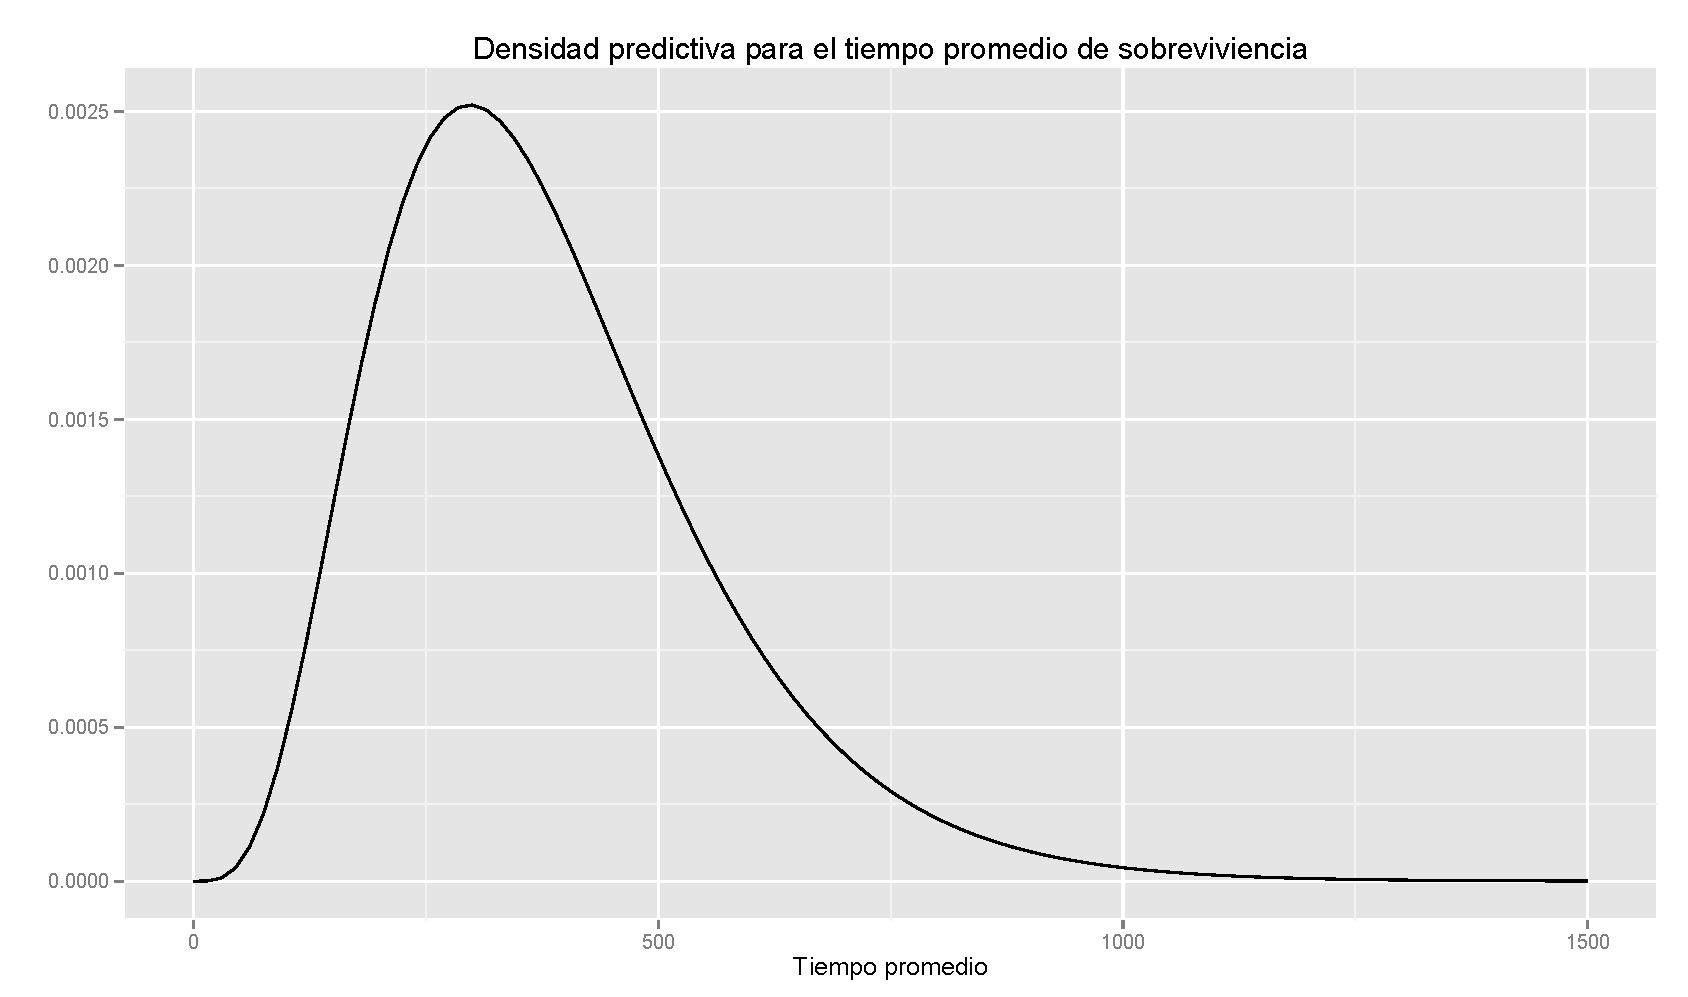
\includegraphics[scale=0.4]{predexponencial.pdf}
    \caption{\emph{Distribuci\'on predictiva posterior para el tiempo promedio de sobrevivencia de transplante de coraz\'on.}}
    \label{pred_post_expo_eje}
    \end{figure}
    
    \section{Modelo normal con media desconocida y varianza conocida}
    
    En esta dos \'ultimas secciones de este cap\'itulo, se considera datos que pueden ser descritos adecuadamente con la distribuci\'on normal, la cual se diferencia de las anteriores distribuciones consideradas pues tiene dos par\'ametros. En el siguiente cap\'itulo se considera el caso general cuando ambos par\'ametros son desconocidos. En esta parte, se asume que la varianza te\'orica es conocica, y el objetivo es estimar la media te\'orica.
    
    Suponga que $Y_1,\cdots,Y_n$ son variables independientes e id\'enticamente distribuidos con distribuci\'on $Normal(\theta,\sigma^2)$ con $\theta$ desconcido pero $\sigma^2$ conocido. De esta forma, la funci\'on de verosimilitud de los datos est\'a dada por
    \begin{align}
    \label{vero_normal}
    p(\mathbf{Y} \mid \theta)&=\prod_{i=1}^n\frac{1}{\sqrt{2\pi\sigma^2}}\exp\left\{-\frac{1}{2\sigma^2}(y_i-\theta)^2\right\}I_\mathbb{R}(y)\notag\\
    &=(2\pi\sigma^2)^{-n/2}\exp\left\{-\frac{1}{2\sigma^2}\sum_{i=1}^n(y_i-\theta)^2\right\}
    \end{align}
    
    Como el par\'ametro $\theta$ puede tomar cualquier valor en los reales, es posible asignarle una distribuci\'on previa $\theta \sim Normal(\mu,\tau^2)$. Bajo este marco de referencia se tienen los siguientes resultados
    
    \begin{Res}\label{Res_pos_theta}
    La distribuci\'on posterior del par\'ametro de inter\'es $\theta$ sigue una distribuci\'on
    \begin{equation*}
    \theta|\mathbf{Y} \sim Normal(\mu_n,\tau^2_n).
    \end{equation*}
    En donde
    \begin{equation}\label{tau_sigma_n}
    \mu_n=\frac{\frac{n}{\sigma^2}\bar{Y}+\frac{1}{\tau^2}\mu}{\frac{n}{\sigma^2}+\frac{1}{\tau^2}}
    \ \ \ \ \ \ \ \text{y} \ \ \ \ \ \ \
    \tau_n^2=\left(\frac{n}{\sigma^2}+\frac{1}{\tau^2}\right)^{-1}
    \end{equation}
    \end{Res}
    
    \begin{proof}
    \begin{align*}
    p(\theta \mid \mathbf{Y})&\propto p(\mathbf{Y} \mid \theta)p(\theta \mid \mu,\tau^2)\\
    &\propto \exp\left\{-\frac{1}{2\sigma^2}\sum_{i=1}^n(y_i-\theta)^2-\frac{1}{2\tau^2}(\theta-\mu)^2\right\}\\
    &= \exp\left\{-\frac{1}{2}\left[\frac{\sum_{i=1}^n(y_i-\theta)^2}{\sigma^2}+\frac{(\theta-\mu)^2}{\tau^2}\right]\right\}\\
    &\propto \exp\left\{-\frac{1}{2}\left[\frac{n\theta^2}{\sigma^2}-\frac{2\theta\sum_{i=1}^ny_i}{\sigma^2}+\frac{\theta^2}{\tau^2}-\frac{2\theta\mu}{\tau^2}\right]\right\}\\
    &= \exp\left\{-\frac{\theta^2}{2}\left[\frac{n}{\sigma^2}+\frac{1}{\tau^2}\right]+
    \theta\left[\frac{n\bar{y}}{\sigma^2}+\frac{\mu}{\tau^2}\right]\right\}\\
    &= \exp\left\{-\frac{\theta^2}{2\tau^2_n}+\frac{\theta\mu_n}{\tau_n^2}\right\}\\
    &= \exp\left\{-\frac{1}{2\tau^2_n}(\theta^2-2\theta\mu_n)\right\}\\
    &\propto \exp\left\{-\frac{1}{2\tau^2_n}(\theta^2-2\theta\mu_n+\mu_n^2)\right\}\\
    &= \exp\left\{-\frac{1}{2\tau^2_n}(\theta-\mu_n)^2\right\}
    \end{align*}
    Por lo tanto, se encuentra una expresi\'on id\'entica a la funci\'on de distribuci\'on de una variable aleatoria con distribuci\'on $Normal(\mu_n,\tau_n^2)$.
    \end{proof}
    
    Observando la forma de $\mu_n$, que corresponde a la estimaci\'on bayesiana del par\'ametro $\theta$, podemos concluir que \'este es una combinaci\'on convexa entre el estimador cl\'asico de m\'axima verosimlitud $\hat{\theta}_C=\bar{y}$ y el estimador previo $\hat{\theta}_P=\mu$, puesto que:
    \begin{align*}
    \hat{\theta}_B=\mu_n&=\frac{\frac{n}{\sigma^2}\bar{Y}+\frac{1}{\tau^2}\mu}{\frac{n}{\sigma^2}+\frac{1}{\tau^2}}\\
    &=\frac{\frac{n}{\sigma^2}}{\frac{n}{\sigma^2}+\frac{1}{\tau^2}}\bar{Y}+\frac{\frac{1}{\tau^2}}{\frac{n}{\sigma^2}+\frac{1}{\tau^2}}\mu\\
    &=\frac{\frac{n}{\sigma^2}}{\frac{n}{\sigma^2}+\frac{1}{\tau^2}}\hat{\theta}_C+\frac{\frac{1}{\tau^2}}{\frac{n}{\sigma^2}+\frac{1}{\tau^2}}\hat{\theta}_P\\
    \end{align*}
    
    De donde se puede concluir que para una distribuci\'on previa fija, entre mayor sea el tama\~no muestral $n$, m\'as peso tendr\'a el estimador cl\'asico $\hat{\theta}_C$ en el c\'alculo del estimador bayesiano. De la misma forma, para un conjunto fijo de datos $\mathbf{Y}$, entre menor sea la varianza previa, $\tau^2$, m\'as certeza tenemos sobre la informaci\'on previa y por consiguiente la estimaci\'on bayesiana $\mu_n$ se acercar\'a m\'as a la estimaci\'on previa. En la Figura \ref{compara_normal} se observa la funci\'on de densidad previa, funci\'on de verosimilitud y funci\'on de densidad posterior con $\mu=5$, $\tau^2=0.01$, $\bar{y}=2$, $\sigma^2=1$ y $n=5,10,50,200$. Podemos observar que a medida que el tama\~no muestral $n$ aumente, la funci\'on de verosimilitud (vista como la funci\'on del par\'ametro $\theta$) se vuelve m\'as concentrada alrededor del valor de $\bar{y}$, y a consecuencia, la funci\'on de densidad posterior de $\theta$ se sit\'ua m\'as cercana a la funci\'on de verosimilitud, y la estimaci\'on bayesiana se acerca m\'as a la estimaci\'on cl\'asica $\bar{y}$.
    
    \begin{figure}[!h]
    \centering
    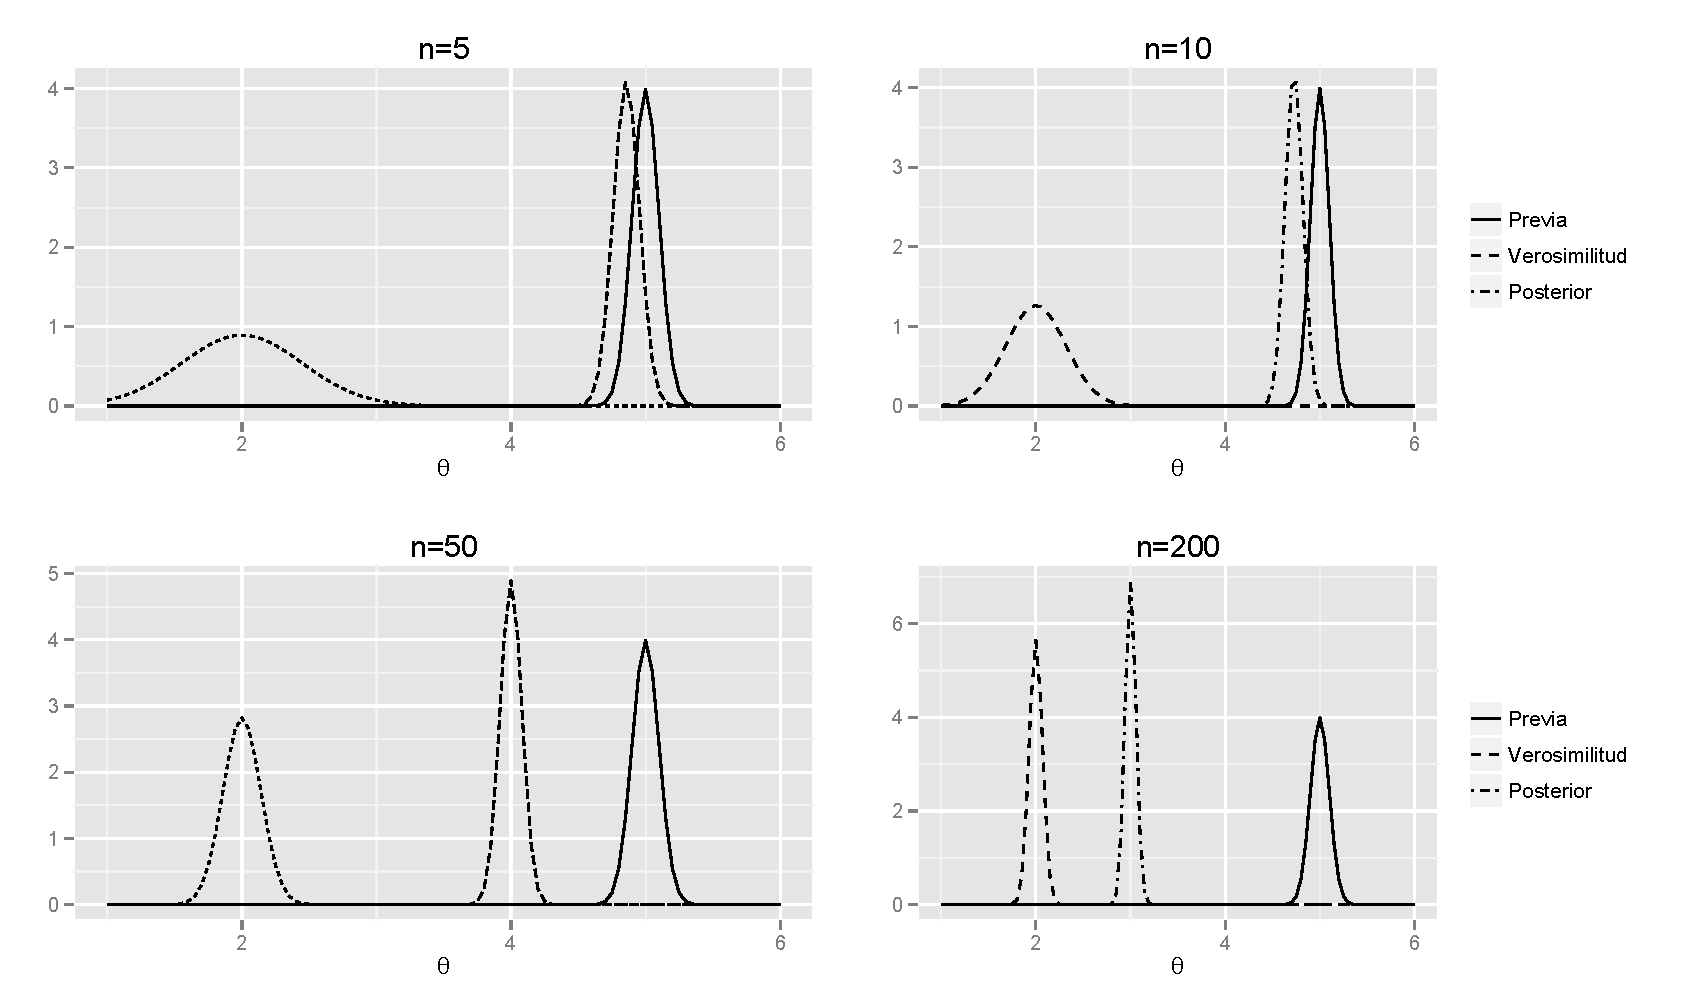
\includegraphics[scale=0.57]{Comparacion_Normal.pdf}
    \caption{\emph{Distribuci\'on previa, funci\'on de verosimilitud y distribuci\'on posterior del par\'ametro $\theta$ con $\mu=5$, $\tau^2=0.01$, $\bar{y}=2$, $\sigma^2=1$ y $n=5,10,50,200$.}}
    \label{compara_normal}
    \end{figure}
    
    \textbf{\emph{Distribuci\'on previa no informativa para $\theta$}}
    
    Por otro lado, n\'otese que en el caso en donde de antemano se desconozca el comportamiento estructural de $\theta$, es posible hacer su distribuci\'on previa tan plana y vaga como sea posible. Para esto, basta con hacer tender al par\'ametro de precisi\'on de la distribuci\'on previa hacia infinito. Es decir $\tau^2 \longrightarrow \infty$, en este caso, la distribuci\'on previa de $\theta$ corresponde a una distribuci\'on impropia, $p(\theta)\propto cte$. Esta idea intuitiva para representar la falta de la informaci\'on previa corresponde a la previa no informativa de Jeffreys, puesto que la informaci\'on de Fisher del par\'ametro $\theta$ en una variable con distribuci\'on normal est\'a dada por 
    \begin{equation*}
    I(\theta)=1/\sigma^2
    \end{equation*}
    
    De donde se puede concluir qua la previa no informativa de Jeffreys est\'a dada por 
    \begin{equation*}
    p(\theta)\propto 1/\sigma\propto cte
    \end{equation*}
    
    Se puede ver que cuando se utiliza la anterior distribuci\'on previa para $\theta$, la distribuci\'on posterior est\'a dada por (Ejercicio \ref{XXX})
    \begin{equation*}
    \theta\mid\mathbf{Y}\sim Normal\left(\bar{y},\ \dfrac{\sigma^2}{n}\right)
    \end{equation*}
    
    Finalmente, comparemos los resultados inferenciales obtenidos con la previa no informativa de Jeffreys con el enfoque inferencial cl\'asico en t\'erminos de la estimaci\'on puntua y el intervalo de credibilidad y de confianza.
    
    \begin{itemize}
    \item En cuanto a la estimaci\'on puntual, es claro que ambos enfoques conducen al mismo estimador $\hat{\theta}=\bar{Y}$.
    \item Con respecto al intervalo para el par\'ametro $\theta$, al usar el enforque bayesiano con la previa no informativa de   Jeffreys, un intervalo de credibilidad de $(1-\alpha)\times 100\%$ est\'an dadas por los percentiles $\alpha/2$ y $1-\alpha   /2$ de la distribuci\'on posterior de $\theta$: $Normal(\bar{y},\sigma^2/n)$, denotaremos estos percentiles como $a$ y $b$, respectivamente. 
    Por definici\'on tenemos que, si $X\sim N(\bar{y},\sigma^2/n)$,
    \begin{align*}
    \alpha/2&=Pr(X<a)\\
    &=Pr(\frac{X-\bar{y}}{\sigma/\sqrt{n}}<\frac{a-\bar{y}}{\sigma/\sqrt{n}})\\
    &=Pr(Z < \frac{a-\bar{y}}{\sigma/\sqrt{n}})
    \end{align*}
    Estos es, $\frac{a-\bar{y}}{\sigma/\sqrt{n}}$ es el percentil $\alpha/2$ de la distribuci\'on normal est\'andar $z_{\alpha/2}$ \'o equivalentemente $-z_{1-\alpha/2}$. De esta forma, tenemos que $a=\bar{y}-z_{1-\alpha/2}\sigma/\sqrt{n}$. An\'alogamente tenemos que $b=bar{y}+z_{1-\alpha/2}\sigma/\sqrt{n}$, y podemos concluir que un intervalo de crediblidad de $(1-\alpha)\times 100\%$ est\'a dada por $\bar{y}\pm z_{1-\alpha/2}\sigma/\sqrt{n}$, el cual coincide con el intervalo de confianza para $\theta$ usando el enfoque de la inferencia cl\'asica \cite{Zhang}.
    \end{itemize}
    
    Ahora revisamos las diferentes formas de hallar la distribuci\'on previa para $\theta$. En primer lugar, consideramos el caso cuando la informaci\'on previa se encuentra en un conjunto de datos $x_1,\cdots,x_{m}$ que corresponden a mediciones de la variable de estudio $Y$ en otro punto de tiempo, en otro punto geogr\'afico, o inclusive en otra poblaci\'on de estudio. En este caso, podemos tomar la media de la distribuci\'on previa $\mu$ como $\bar{X}$ y la varianza de la distribuci\'on previa $\tau^2$ como $S^2_X$.
    
    En el caso de que no se dispongan de datos como informaci\'on previa, sino que \'esta est\'a contenida en alguna estimaci\'on que se haya realizado sobre $\theta$. Por ejemplo, si se dispone de alg\'un modelamiento estad\'istico que se haya hecho previamente sobre $\theta$, podemos f\'acilmente obtener el valor estimado de $\theta$ y el error est\'andar de esta estimaci\'on, y naturalmente, estos dos valores ser\'ian nuestros par\'ametros de la distribuci\'on previa: $\mu$ y $\tau^2$. 
    
    Finalmente, si la estimaci\'on previa de $\theta$ se presentada en forma de un intervalo, por ejemplo, si se sabe que un intervalo de confianza para $\theta$ es $(15.3,\ 24.7)$, entonces podemos usar $\mu$ como el punto medio de este intervalo, es decir, $\mu=20$ y para escoger el valor de $\tau^2$, se tiene en cuenta que en muchas ramas de la estad\'istica, un intervalo de confianza se puede aproximar por $\hat{\theta}\pm 2\sqrt{var(\hat{\theta})}$. De esta forma, podemos usar $\tau^2=\left(\frac{24.7-20}{2}\right)^2\approx5.5$
    
    En cuanto a las distribuciones predictivas, a continuaci\'on se encuentran las expresiones correspondientes para una observaci\'on o una nueva muestra.
    
    \begin{Res}
    La distribuci\'on predictiva previa para una observaci\'on $y$ es
    \begin{equation*}
    y \sim Normal (\mu, \tau^2+\sigma^2)
    \end{equation*}
    \end{Res}
    
    \begin{proof}
    De la definici\'on de funci\'on de distribuci\'on predictiva se tiene que
    \begin{align*}
    p(Y)&=\int p(Y \mid \theta)p(\theta \mid \mu,\tau^2)\ d\theta\\
    &=\int_{-\infty}^{\infty} \frac{1}{\sqrt{2\pi\sigma^2}}\exp\left\{-\frac{1}{2\sigma^2}(y-\theta)^2\right\}
    \frac{1}{\sqrt{2\pi\tau^2}}\exp\left\{-\frac{1}{2\tau^2}(\theta-\mu)^2\right\}d\theta\\
    \end{align*}
    
    \citeasnoun{Berger} desarroll\'o las siguientes igualdades
    \begin{align*}
    &\ \ \ \ \frac{1}{2}\left[\frac{(\theta-\mu)^2}{\tau^2}+\frac{(y-\theta)^2}{\sigma^2}\right]\\
    &=\frac{1}{2}\left[\left(\frac{1}{\tau^2}+\frac{1}{\sigma^2}\right)\theta^2-2\left(\frac{\mu}{\tau^2}+\frac{y}{\sigma^2}\right)\theta+\left(\frac{\mu^2}{\tau^2}+\frac{y^2}{\sigma^2}\right)\right]\\
    &=\frac{1}{2\tau_1^2}\left[\theta^2-2\tau_1^2\left(\frac{\mu}{\tau^2}+\frac{y}{\sigma^2}\right)\theta+\tau_1^4\left(\frac{\mu}{\tau^2}+\frac{y}{\sigma^2}\right)^2\right]+\frac{1}{2}\left(\frac{\mu^2}{\tau^2}+\frac{y^2}{\sigma^2}\right)-\frac{\tau_1^2}{2}\left(\frac{\mu}{\tau^2}+\frac{y}{\sigma^2}\right)^2\\
    &=\frac{1}{2\tau_1^2}\left[\theta-\tau_1^2\left(\frac{\mu}{\tau^2}+\frac{y}{\sigma^2}\right)\right]^2+\frac{1}{2}\left[\left(\frac{1}{\sigma^2}-\frac{\tau_1^2}{\sigma^4}\right)y^2-2\frac{\mu\tau_1^2}{\tau^2\sigma^2}y+\left(\frac{\mu^2}{\tau^2}-\frac{\mu^2\tau_1^2}{\tau^4}\right)\right]\\
    &=\frac{1}{2\tau_1^2}\left[\theta-\mu_1\right]^2+\frac{1}{2}\left[\frac{1}{\sigma^2+\tau^2}y^2-2\frac{\mu}{\sigma^2+\tau^2}y+\frac{\mu^2}{\sigma^2+\tau^2}\right]\\
    &=\frac{1}{2\tau_1^2}\left[\theta-\mu_1\right]^2+\frac{1}{2(\sigma^2+\tau^2)}(y-\mu)^2.
    \end{align*}
    
    
    Entonces
    \begin{align*}
    p(Y)&=\int_{-\infty}^{\infty} \frac{1}{2\pi\sigma\tau}\exp\left\{-\frac{1}{2\tau_1^2}(\theta-\mu_1)^2\right\}
    \exp\left\{-\frac{1}{2(\tau^2+\sigma^2)}(y-\mu)^2\right\}d\theta\\
    &= \frac{1}{\sqrt{2\pi\frac{\sigma^2\tau^2}{\tau_1^2}}}\exp\left\{-\frac{1}{2(\tau^2+\sigma^2)}(y-\mu)^2\right\}
    \int_{-\infty}^{\infty} \frac{1}{\sqrt{2\pi\tau_1^2}}\exp\left\{-\frac{1}{2\tau_1^2}(\theta-\mu_1)^2\right\}d\theta\\
    &= \frac{1}{\sqrt{2\pi(\tau^2+\sigma^2)}}\exp\left\{-\frac{1}{2(\tau^2+\sigma^2)}(y-\mu)^2\right\}
    \end{align*}
    \end{proof}
    
    Una vez recolectados los datos $\mathbf{Y}=\{Y_1,\cdots,Y_n\}$, se obtiene la distribuci\'on predictiva posterior dada en el siguiente resultado. La demostraci\'on es similar al del resultado anterior, y se deja como ejercicio para los lectores.
    \begin{Res}\label{pred_y_theta}
    La distribuci\'on predictiva posterior para una nueva observaci\'on $\tilde{y}$ es
    \begin{equation*}
    \tilde{y} \mid \mathbf{Y} \sim Normal (\mu_n, \tau_n^2+\sigma^2)
    \end{equation*}
    
    cuando se tiene una distribuci\'on previa informativa para $\theta$. 
    
    Cuando se utiliza la distribuci\'on previa no informativa de Jeffreys, la distribuci\'on predictiva posterior para una nueva observaci\'on $\tilde{y}$ es
    \begin{equation*}
    \tilde{y} \mid \mathbf{Y} \sim Normal \left(\bar{y}, \left(1+\dfrac{1}{n}\right)\sigma^2\right)
    \end{equation*}
    \end{Res}
    
    \begin{proof}
    \label{Res_pred_normal}
    Se deja como ejercicio para los lectores.
    \end{proof}
    
    En algunas situaciones, se quiere conocer el comportamiento probabil\'istico de m\'as de una nueva observaci\'on, digamos $Y_1^*,\cdots,Y_{n^*}^*$, en este caso, lo ideal ser\'ia obtener la distribuci\'on conjunta predictiva posterior de la nueva muestra, $p(Y_1^*,\cdots,Y_{n^*}^*|\mathbf{Y})$. Sin embargo, esta distribuci\'on no es f\'acil de hallar, y procedemos a hallar la distribuci\'on predictiva posterior de la media de esta nueva muestra $\bar{Y}^*$, la cual es dada en el siguiente resultado. 
    
    \begin{Res}\label{pred_norm}
    La distribuci\'on predictiva posterior para la media muestral $\bar{Y}^*$ de una nueva muestra es 
    \begin{equation*}
    \bar{Y}^*|\mathbf{Y}\ \sim N\left(\mu_n, \frac{\sigma^2}{n^*}+\tau^2_n\right)
    \end{equation*}
    cuando se tiene una previa informativa para $\theta$, $\mu_n$ y $\tau^2_n$ fueron definidos en (\ref{tau_sigma_n}).
    
    Cuando se utiliza la distribuci\'on previa no informativa de Jeffreys para $\theta$, la distribuci\'on predictiva posterior para la media muestral $\bar{Y}^*$ de una nueva muestra es 
    \begin{equation*}
    \bar{Y}^*|\mathbf{Y}\ \sim N\left(\bar{y}, \left(\dfrac{1}{n}+\dfrac{1}{n^*}\right)\sigma^2\right).
    \end{equation*}
    \end{Res}
    
    \begin{proof}
    Primero, consideramos cuando la distribuci\'on previa de $\theta$ es $N(\mu,\tau^2)$, tenemos que:
    \begin{align*}
    p(\bar{Y}^*|\mathbf{Y})&=\int_{-\infty}^\infty p(\bar{Y}^*|\theta)p(\theta|\mathbf{Y})\ d\theta\\
    &=\int_{-\infty}^\infty (2\pi\frac{\sigma^2}{n^*})^{-1/2}\exp\left\{-\frac{n^*}{2\sigma^2}(\bar{y}^*-\theta)^2\right\}
    (2\pi\tau_n^2)^{-1/2}\exp\left\{-\frac{1}{2\tau_n^2}(\theta-\mu_n)^2\right\}\ d\theta\\
    &=\int_{-\infty}^\infty (2\pi)^{-1}(\frac{\sigma^2}{n^*}\tau_n^2)^{-1/2}\exp\left\{-\frac{1}{2}\left[\frac{(\bar{y}^*-\theta)^2}{\sigma^2/n^*}+\frac{(\theta-\mu_n)^2}{\tau^2_n}\right]\right\}\ d\theta\\
    &=\underbrace{\int_{-\infty}^\infty(2\pi\frac{1}{n^*/\sigma^2+1/\tau^2_n})^{-1/2}\exp\left\{-\frac{1}{2}\left(\frac{n^*}{\sigma^2}+\frac{1}{\tau^2_n}\right)\left(\theta-\frac{\bar{y}^*/(\sigma^2/n^*)+\mu_n/\tau^2_n}{n^*/\sigma^2+1/\tau^2_n}\right)^2\right\}\ d\theta}_{\text{igual a 1}}\\
    &\ \ \ \ \ \ \ (2\pi)^{-1/2}(\frac{\sigma^2}{n^*}\tau_n^2)^{-1/2}(\frac{n^*}{\sigma^2}+\frac{1}{\tau^2_n})^{-1/2}\exp\left\{-\frac{1}{2(\sigma^2/n^*+\tau^2_n)}(\bar{y}^*-\mu_n)^2\right\}\\
    &=(2\pi)^{-1/2}(\frac{\sigma^2}{n^*}\tau_n^2)^{-1/2}(\frac{n^*}{\sigma^2}+\frac{1}{\tau^2_n})^{-1/2}\exp\left\{-\frac{1}{2(\sigma^2/n^*+\tau^2_n)}(\bar{y}^*-\mu_n)^2\right\}\\
    &=(2\pi)^{-1/2}(\frac{\sigma^2}{n^*}+\tau^2_n)^{-1/2}\exp\left\{-\frac{1}{2(\sigma^2/n^*+\tau^2_n)}(\bar{y}^*-\mu_n)^2\right\}
    \end{align*}
    
    Los desarrollos para cuando se utiliza la distribuci\'on previa no informativa de Jeffreys es similar, y se deja para los lectores (Ejercicio \ref{Ejer_pre_Jeffreys}). 
    \end{proof}
    
    Del anterior resultado, podemos observar que: (1) la esperanza de la distribuci\'on de $\bar{Y}^*|\mathbf{Y}$ es igual a la esperanza de $\theta|\mathbf{Y}$, y (2) a diferencia de la varianza de $\theta|\mathbf{Y}$, la varianza de $\bar{Y}^*|\mathbf{Y}$ tiene un componente adicional: $\sigma^2/n^*$, de esta forma, tenemos tres fuentes de incertidumbre al momento de pronosticar $\bar{Y}^*$: la incertidumbre en la informaci\'on previa, la incertidumbre en la muestra observada y la incertidumbre en la nueva muestra.
    
    \begin{Eje}\label{eje_vidrios}
    En \citeasnoun[Ejemplo 2.3.6]{Zhang} reportan datos sobre el grosor de l\'aminas de vidrio templado de 3cm para controlar la calidad de los vidrios producidos por una l\'inea de producci\'on con el fin de conocer el grosor real de las l\'aminas producidas. Estos datos son: 3.56, 3.36, 2.99, 2.71, 3.31, 3.68, 2.78, 2.95, 2.82, 3.45, 3.42 y 3.15, con el promedio de 3.18cm. Suponga que por especificaciones t\'ecnicas, se conoce que la varianza del grosor es de $0.1\text{cm}^2$. Por otro lado como informaci\'on previa, se conoce que en la \'ultima inspecci\'on de calidad, se conoce que el grosor promedio fue de 2.8cm con una desviaci\'on est\'andar de 0.23cm.
    
    De la anterior informaci\'on, se puede decir que el par\'ametro de inter\'es $\theta$ ser\'ia el grosor promedio de las l\'aminas. Tambi\'en podemos afirmar que $\sigma^2=0.1cm^2$, $\bar{y}=3.18cm$, $n=12$, y los par\'ametros de la distribuci\'on previa est\'an dados por $\mu=2.8cm$ y $\tau=0.45cm$, de esta forma, podemos calcular los par\'ametros de la distribuci\'on posterior
    \begin{align*}
    \mu_n&=\dfrac{\frac{12}{0.1}\times 3.18+\frac{1}{0.23^2}\times 2.8}{\frac{12}{0.1}+\frac{1}{0.23^2}}=3.13cm\\
    \tau^2_n&=\left(\frac{12}{0.1}+\frac{1}{0.23^2}\right)^{-1}=0.007cm^2\\
      \tau^2&=\sqrt{0.007cm^2}=0.084cm\\
    \end{align*}
    
    Entonces la distribuci\'on posterior del grosor promedio es $N(\mu_n=3.13cm,\ \tau^2_n=0.007cm^2)$. Podemos concluir que la estimaci\'on bayesiana del par\'ametro corresponde a $3.13cm$, mientras que para calcular un intervalo de credibilidad de $95\%$ para el par\'ametro de inter\'es, se debe calcular los percentiles $2.5\%$ y $97.5\%$ de la distribuci\'on posterior de $\theta$, y el intervalo de credibilidad queda dado por $(2.966cm,\ 3.293cm)$.
    
    A continuaci\'on se ilustra el uso de \verb'JAGS' para obtener la estimaci\'on bayesiana del par\'ametro $\theta$.
    
\begin{knitrout}
\definecolor{shadecolor}{rgb}{0.933, 0.933, 0.933}\color{fgcolor}\begin{kframe}
\begin{alltt}
\hlstd{Norm.model} \hlkwb{<-} \hlkwa{function}\hlstd{()\{}
\hlkwa{for}\hlstd{(i} \hlkwa{in} \hlnum{1} \hlopt{:} \hlstd{n)}
\hlstd{\{}
\hlstd{y[i]} \hlopt{~} \hlkwd{dnorm}\hlstd{(theta,} \hlnum{1}\hlopt{/}\hlnum{0.1}\hlstd{)}
\hlstd{\}}
\hlstd{theta} \hlopt{~} \hlkwd{dnorm}\hlstd{(}\hlnum{2.8}\hlstd{,} \hlnum{1}\hlopt{/}\hlstd{(}\hlnum{0.23}\hlopt{^}\hlnum{2}\hlstd{) )}
\hlstd{\}}

\hlstd{n} \hlkwb{<-} \hlnum{12}
\hlstd{y} \hlkwb{<-} \hlkwd{c}\hlstd{(}\hlnum{3.56}\hlstd{,} \hlnum{3.36}\hlstd{,} \hlnum{2.99}\hlstd{,} \hlnum{2.71}\hlstd{,} \hlnum{3.31}\hlstd{,} \hlnum{3.68}\hlstd{,} \hlnum{2.78}\hlstd{,} \hlnum{2.95}\hlstd{,} \hlnum{2.82}\hlstd{,} \hlnum{3.45}\hlstd{,} \hlnum{3.42}\hlstd{,} \hlnum{3.15}\hlstd{)}

\hlstd{Norm.data} \hlkwb{<-} \hlkwd{list}\hlstd{(}\hlstr{"y"}\hlstd{,}\hlstr{"n"}\hlstd{)}
\hlstd{Norm.param} \hlkwb{<-} \hlkwd{c}\hlstd{(}\hlstr{"theta"}\hlstd{)}
\hlstd{Norm.inits} \hlkwb{<-} \hlkwa{function}\hlstd{()\{}
\hlkwd{list}\hlstd{(}\hlstr{"theta"}\hlstd{=}\hlkwd{c}\hlstd{(}\hlnum{3.2}\hlstd{))}
\hlstd{\}}

\hlstd{Norm.fit} \hlkwb{<-} \hlkwd{jags}\hlstd{(}\hlkwc{data}\hlstd{=Norm.data,} \hlkwc{inits}\hlstd{=Norm.inits, Norm.param,} \hlkwc{n.iter}\hlstd{=}\hlnum{10000}\hlstd{,}
\hlkwc{n.burnin}\hlstd{=}\hlnum{1000}\hlstd{,} \hlkwc{model.file}\hlstd{=Norm.model)}
\end{alltt}


{\ttfamily\noindent\itshape\color{messagecolor}{\#\# module glm loaded}}\begin{verbatim}
## Compiling model graph
##    Resolving undeclared variables
##    Allocating nodes
## Graph information:
##    Observed stochastic nodes: 12
##    Unobserved stochastic nodes: 1
##    Total graph size: 45
## 
## Initializing model
\end{verbatim}
\begin{alltt}
\hlkwd{print}\hlstd{(Norm.fit)}
\end{alltt}
\begin{verbatim}
## Inference for Bugs model at "/var/folders/n7/01szs8_x7pq1bvpwwnvq7w_w0000gn/T//Rtmph2sfkH/model15eea40f4d8d4.txt", fit using jags,
##  3 chains, each with 10000 iterations (first 1000 discarded), n.thin = 9
##  n.sims = 3000 iterations saved
##          mu.vect sd.vect  2.5%   25%   50%   75%  97.5%  Rhat n.eff
## theta      3.132   0.085 2.965 3.073 3.132 3.190  3.297 1.001  3000
## deviance   7.331   1.583 6.170 6.285 6.710 7.762 11.824 1.001  3000
## 
## For each parameter, n.eff is a crude measure of effective sample size,
## and Rhat is the potential scale reduction factor (at convergence, Rhat=1).
## 
## DIC info (using the rule, pD = var(deviance)/2)
## pD = 1.3 and DIC = 8.6
## DIC is an estimate of expected predictive error (lower deviance is better).
\end{verbatim}
\end{kframe}
\end{knitrout}
    De donde podemos ver que la estimaci\'on bayesiana de $\theta$ es $3.132cm$ con un error est\'andar de $0.085cm$, mientras que un intervalo de credibilidad del 95\% es $(2.965cm,\ 3.297cm)$, resultados muy similares a lo obtenido calculando directamente $\mu_n$ y $\tau_n$.
    
    Finalmente, ilustramos el uso de la distribuci\'on predictiva posterior. Suponga que la f\'abrica debe hacer un despacho de 8 l\'aminas, y se quiere conocer sobre el grosor promedio del despacho $\bar{y}^*$. Usando el resultado \ref{pred_norm}, tenemos que la disribuci\'on de $\bar{Y}^*$ condicionado en los 12 datos observados est\'a dado por 
    \begin{equation*}
    \bar{Y}^*|\mathbf{Y}\ \sim N\left(\mu_n,\ \frac{\sigma^2}{n^*}+\tau^2_n\right) = N\left(3.13cm,\ \frac{0.1}{8}+0.007\ cm^2\right) = N(3.13cm,\ 0.0195cm^2)
    \end{equation*}
    
    De esta forma, podemos afirmar que el grosor promedio del despacho es de 3.13cm con un intervalo de 95\% dado por los percentiles 2.5\% y 97.5\% de la anterior distribuci\'on: (2.85cm, 3.40cm). N\'otese que el intervalo para $\bar{Y}^{*}$ es m\'as ancho que el intervalo para $\theta$, pues este tiene una varianza mayor a la varianza de la distribuci\'on posterior de $\theta$.
    
    Tambi\'en podemos calcular el intervalo para $\bar{Y}^*$ desde el punto de vista de simulaci\'on, simulando valores de $\theta$ desde su distribuci\'on posterior, y luego simulando valores de $\bar{Y}^*$ desde $p(\bar{Y}^*\mid\theta)$. Los siguientes c\'odigos implemtan este enforque con 5000 iteraciones. Podemos ver que los resultados obtenidos son casi id\'enticos a los calculados anteriormente.
\begin{knitrout}
\definecolor{shadecolor}{rgb}{0.933, 0.933, 0.933}\color{fgcolor}\begin{kframe}
\begin{alltt}
\hlstd{y.bar} \hlkwb{<-} \hlkwd{c}\hlstd{()}
\hlstd{mu.n} \hlkwb{<-} \hlnum{3.13}\hlstd{; tau2.n} \hlkwb{<-} \hlnum{0.007}\hlstd{; sigma2} \hlkwb{<-} \hlnum{0.1}
\hlkwa{for}\hlstd{(i} \hlkwa{in} \hlnum{1}\hlopt{:}\hlnum{5000}\hlstd{)\{}
  \hlstd{theta} \hlkwb{<-} \hlkwd{rnorm}\hlstd{(}\hlnum{1}\hlstd{, mu.n,} \hlkwd{sqrt}\hlstd{(tau2.n))}
  \hlstd{y.bar[i]} \hlkwb{<-} \hlkwd{rnorm}\hlstd{(}\hlnum{1}\hlstd{, theta,} \hlkwd{sqrt}\hlstd{(sigma2}\hlopt{/}\hlnum{8}\hlstd{))}
\hlstd{\}}
\hlkwd{mean}\hlstd{(y.bar)}
\end{alltt}
\begin{verbatim}
## [1] 3.127
\end{verbatim}
\begin{alltt}
\hlkwd{quantile}\hlstd{(y.bar,} \hlkwd{c}\hlstd{(}\hlnum{0.025}\hlstd{,}\hlnum{0.975}\hlstd{))}
\end{alltt}
\begin{verbatim}
##  2.5% 97.5% 
## 2.853 3.405
\end{verbatim}
\end{kframe}
\end{knitrout}
    \end{Eje}
    
    \section{Modelo normal con varianza desconocida y media conocida}\label{Normal_Varianza}
    
    En esta secci\'on consideramos variables independientes e id\'enticamente distribuidas $Y_1,\cdots,Y_n\sim N(\theta,\sigma^2)$. Asumimos que $\theta$ es conocida y el par\'ametro de inter\'es es $\sigma^2$. En la pr\'actica es inusual encontrar situaciones donde este supuesto se cumpla, sin embargo, los desarrollos presentados en esta secci\'on ser\'an \'utiles en el siguiente cap\'itulo cuando se aborda la distribuci\'on normal con ambos par\'ametros desconocidos. 
    
    Para desarrollar la estimaci\'on bayesiana para $\sigma^2$, el primer paso es asignarle una distribuci\'on previa que sea acorde con los valores que toma el par\'ametro, y en lo posible inducir una distribuci\'on posterior conjugada. De esta forma, observamos que el par\'ametro $\sigma^2$ es estrictamente positivo, y la distribuci\'on previa debe tener soporte \'unicamente los valores positivos. Si bien la distribuci\'on que primero viene a mente ser\'ia la distribuci\'on Gamma, al observar la funci\'on de verosimilitud dada en \ref{vero_normal}, es claro que esta opci\'on no inducir\'a una distribuci\'on posterior conjugado. Por lo tanto recurrimos a la distribuci\'on Inversa-Gamma que tiene la siguiente funci\'on de densidad:
    \begin{equation}\label{densi_Inv_Gamma}
    f(x)=\dfrac{\beta^\alpha}{\Gamma(\alpha)}x^{-\alpha-1}\exp\left\{-\frac{\beta}{x}\right\}
    \end{equation}
    
    para $x>0$. $\alpha>0$ es el par\'ametro de forma y $\beta>0$ es el par\'ametro de escala, y usamos la notacion $X\sim Inversa-Gamma(\alpha,\beta)$. Se tiene que para esta distribuci\'on, $E(X)=\frac{\beta}{\alpha-1}$ cuando $\alpha>1$ y $Var(X)=\frac{\beta^2}{(\alpha-1)^2(\alpha-2)}$ cuando $\alpha>2$.
    
    En la literatura se acostumbra usar la siguiente distribuci\'on previa para el par\'ametro $\sigma^2$:
    \begin{equation*}
    \sigma^2 \sim Inversa-Gamma(n_0/2,\ n_0\sigma^2_0/2)
    \end{equation*}
    
    La esperanza previa $\sigma^2$ viene dada por
    \begin{equation*}
    E(\sigma^2)=\dfrac{\frac{n_0\sigma^2_0}{2}}{\frac{n_0}{2}-1}=\dfrac{n_0\sigma^2_0}{n_0-2}\approx\sigma^2_0
    \end{equation*}
    
    y
    \begin{equation*}
    Var(\sigma^2)=\dfrac{\left(\frac{n_0\sigma^2_0}{2}\right)^2}{\left(\frac{n_0}{2}-1\right)\left(\frac{n_0}{2}-2\right)}\approx \dfrac{2\sigma^4_0}{n_0}
    \end{equation*}
    
    De donde podemos escoger el par\'ametro $\sigma^2_0$ como  el valor que se cree apropiado para $\sigma^2$ con base en la informaci\'on previa. $n_0$ denota el n\'umero de datos en la informaci\'on previa, el cual determina el grado de certidumbre del investigador sobre la informaci\'on previa, pues entre mayor sea $n_0$, mayor cantidad de datos representa la distribuci\'on previa, la varianza previa de $\sigma^2$ se hace menor, lo cual representa menor incertidumbre en la distribuci\'on previa.
    
    En la figura \ref{Priori_Sigma2} podemos observar la forma de la distribuci\'on previa para $\sigma^2$ para diferentes valores de $\sigma^2_0$ y $n_0$. Es claro que la distribuci\'on est\'a concentrada alrededor del valor de $\sigma^2_0$; y para un mismo valor de $\sigma^2_0$, entre mayor sea $n_0$ m\'as concentrada est\'a la funci\'on alrededor de $\sigma^2_0$.
    \begin{figure}[!h]
    \centering
    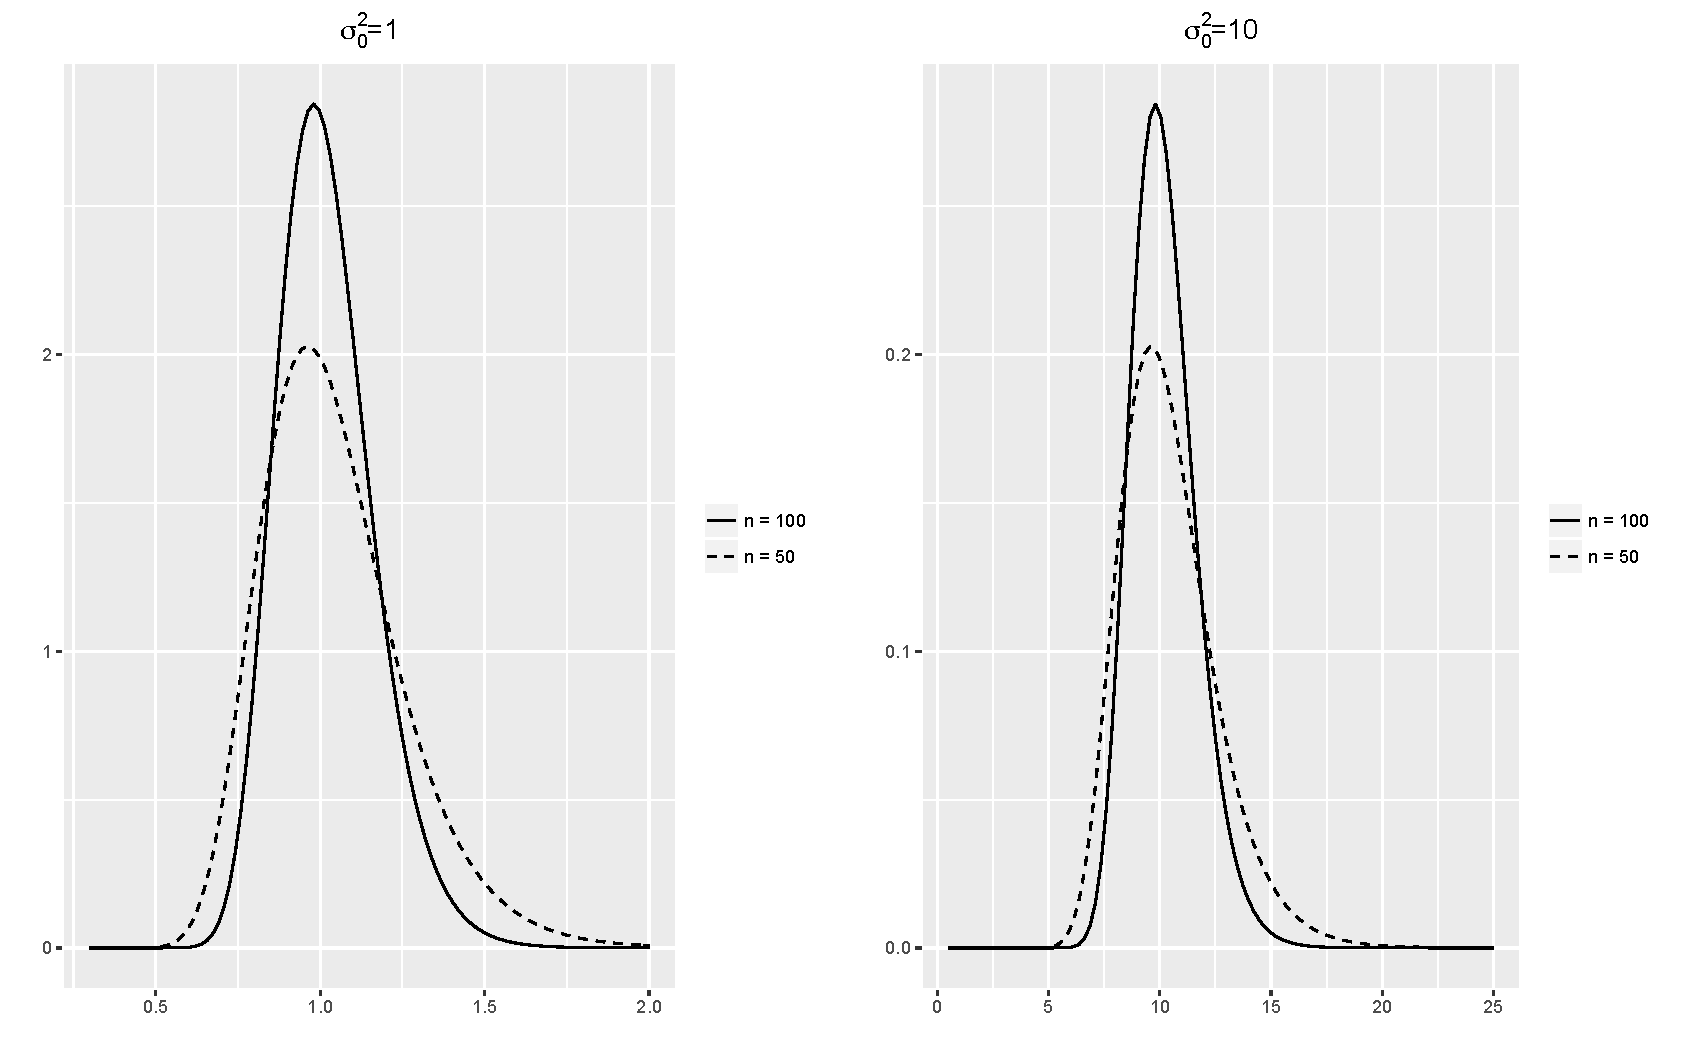
\includegraphics[scale=0.5]{Priori_Sigma2.pdf}
    \caption{\emph{Funci\'on de densidad Inversa-Gamma para diferentes valores de $\sigma^2_0$ y $n_0$.}}
    \label{Priori_Sigma2}
    \end{figure}
    
    Una vez definida la distribuci\'on previa de $\sigma^2$, procedemos a encontrar la distribuci\'on posterior.
    \begin{Res}\label{posterior_sigma2}
    La distribuci\'on posterior de $\sigma^2$ es
    \begin{equation*}
    \sigma^2  \mid \mathbf{Y} \sim Inversa-Gamma\left(\frac{n_0+n}{2},\frac{v_0}{2}\right)
    \end{equation*}
    En donde $v_0=n_0\sigma^2_0+n\hat{\sigma}^2_C$ donde $\hat{\sigma}^2_C=\dfrac{1}{n}\sum_{i=1}^n(y_i-\theta)^2$
    \end{Res}
    
    \begin{proof}
    Acudiendo a la distribuci\'on posterior conjunta e incorporando los t\'erminos que no dependen de $\theta$ en la constante de proporcionalidad, se tiene que
    \begin{align*}
    p(\sigma^2 \mid \mathbf{Y})&\propto p(\sigma^2)p(\mathbf{Y}\mid \sigma^2) \\
    &\propto (\sigma^2)^{-n_0/2-1}\exp\left\{-\dfrac{n_0\sigma_0^2}{2\sigma^2}\right\}(\sigma^2)^{-n/2}\exp\left\{-\frac{1}{2\sigma^2}\sum_{i=1}^n(y_i-\theta)^2\right\}\\
    &= (\sigma^2)^{-(n_0+n)/2-1}\exp\left\{-\frac{1}{2\sigma^2}\left[n_0\sigma_0^2+n\hat{\sigma}^2_C\right]\right\}
    \end{align*}
    
    donde $\hat{\sigma}^2_C$ es el estimador cl\'asico de $\sigma^2$ cuando $\theta$ es conocido, definido como $\hat{\sigma}^2_C=\dfrac{1}{n}\sum_{i=1}^n(y_i-\theta)^2$. De esta forma se encuentra la distribuci\'on posterior de $\sigma^2$.
    \end{proof}
    
    De la distribuci\'on posterior de $\sigma^2$ se puede observar que la estimaci\'on bayesiana de $\sigma^2$ est\'a dada por 
    \begin{align*}
    \hat{\sigma}^2_B&=\dfrac{\frac{v_0}{2}}{\frac{n_0+n}{2}}\\
    &=\dfrac{n_0\sigma^2_0+n\hat{\sigma}^2_C}{n_0+n-2}\\
    &\approx \dfrac{n_0\sigma^2_0+n\hat{\sigma}^2_C}{n_0+n}\\
    &=\dfrac{n_0}{n_0+n}\sigma^2_0+\dfrac{n}{n_0+n}\hat{\sigma}^2_C
    \end{align*}
    
    Esto es, la estimaci\'on bayesiana viene siendo un promedio ponderado entre la estimaci\'on previa $\sigma^2_0$ y la estimaci\'on cl\'asica $\hat{\sigma}^2_C$, y las ponderaciones depende directa y \'unicamente del n\'umero de datos de las dos fuentes de informaci\'on: $n_0$ y $n$. En la figura \ref{Posterior_Sigma2} se muestra la funci\'on de densidad de la distribuci\'on previa, distribuci\'on posterior y la funci\'on de verosimilitud vista como una funci\'on de $\sigma^2$ con $n_0=20$, $\sigma^2_0=10$, $\hat{\sigma}^2_C=50$, el tama??o muestral es $n=5,20,50,100$. Podemos ver que a medida que a medida que el tama\~o muestral $n$ aumenta, la funci\'on de verosimilitud se concentra m\'as alrededor del valor de $\hat{\sigma}^2_C$, y como consecuencia, la funci\'on de densidad posterior de $\sigma^2$ se acerca m\'as a la funci\'on de verosimilitud, y la estimaci\'on bayesiana tambi\'en se asemeja m\'as a la estimaci\'on cl\'asica $\hat{\sigma}^2_C$.
    
    \begin{figure}[!h]
    \centering
    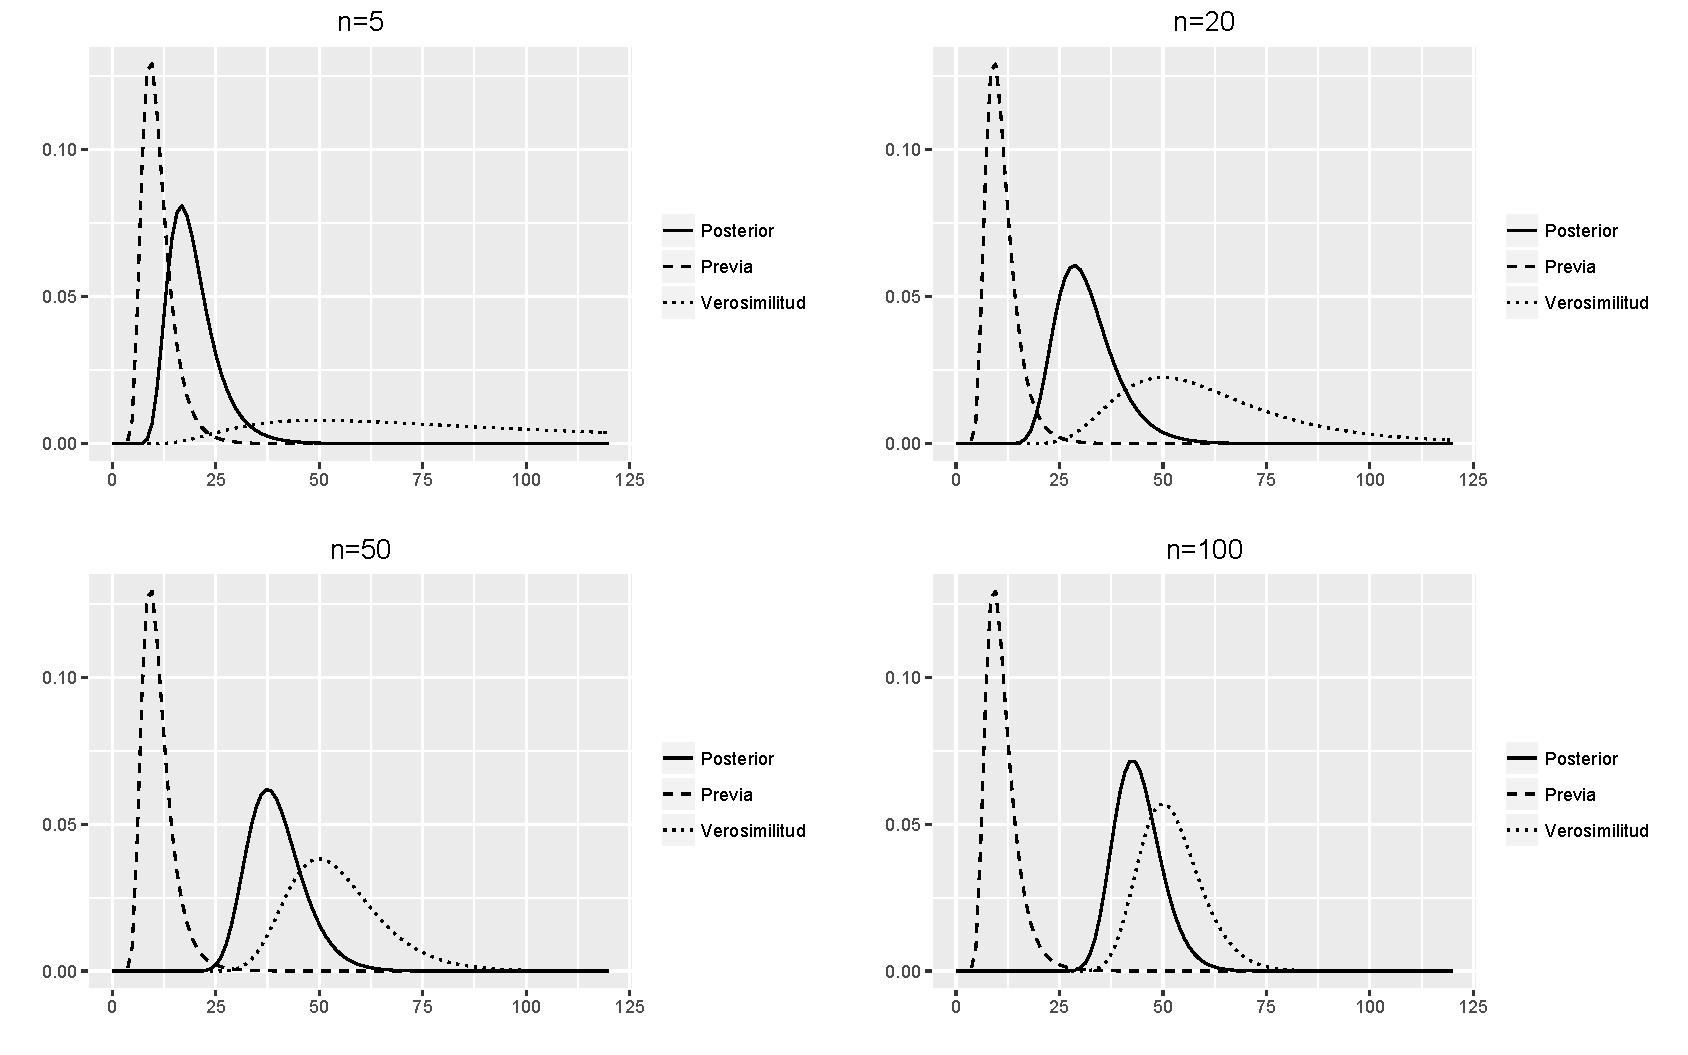
\includegraphics[scale=0.5]{Sigma2_compara.pdf}
    \caption{\emph{Distribuci\'on previa, funci\'on de verosimilitud y distribuci\'on posterior de $\sigma^2$ con $n_0=20$, $\sigma^2_0=10$, $\hat{\sigma}^2_C=50$ y $n=5,20,50,100$.}}
    \label{Posterior_Sigma2}
    \end{figure}
    
    \textbf{\emph{Distribuci\'on previa no informativa para $\sigma^2$}}
    
    Recurriendo a las distribuci\'on previa no informativa de Jeffreys que establece que $p(\theta)\propto I(\theta) ^{1/2}$, donde $\theta$ es el par\'ametro de inter\'es, y $I(\theta)$ es la informaci\'on de Fisher acerca del par\'ametro $\theta$. Despu\'es de algunos c\'alculos se puede ver que (para m\'as detalles, ver \citeasnoun[Sec.2.4]{Zhang}) $I(\sigma^2)=\frac{n}{2\sigma^4}$
    
    De esta forma, la distribuci\'on previa no informativa de Jeffreys est\'a dada por 
    \begin{equation*}
    p(\sigma^2)\propto \sigma^{-2}
    \end{equation*}
    
    para $\sigma^2>0$. En \verb'JAGS' se acostumbra a usar valores peque\~nos de $\alpha$ y $\beta$ para denotar esta distribuci\'on no informativa pues en este caso, la funci\'on de densidad (\ref{densi_Inv_Gamma}) es similar a $p(\sigma^2)\propto \sigma^{-2}$. 
    
        Ahora, si bien esta distribuci\'on previa es una distribuci\'on impropia (pues $\int_0^\infty p(\sigma^2)=\infty$), al combinar con la funci\'on de verosimilitud, se puede concluir que la distribuci\'on posterior de $\sigma^2$ corresponde a una distribuci\'on Inversa-Gamma con el par\'ametro de forma $n/2$, y par\'ametro de escala $n\hat{\sigma}^2_C/2$ (se deja como ejercicio a los lectores). En la figura \ref{Posterior_Sigma2_Jeffreys} se puede observar la funci\'on de densidad previa de Jeffreys (\'este ha sido escalado para la \'optima visualizaci\'on), la funci\'on de verosimilitud con $n=50$, $\hat{\sigma}^2_C=10$ y la funci\'on de densidad posterior resultante. Se puede ver claramente que la forma de la distribuci\'on posterior es muy similar a la funci\'on de verosimilitud, de donde se puede intuir que la estimaci\'on bayesiana resulta similar a la estimaci\'on cl\'asica de $\sigma^2$. Efectivamente, podemos ver que cuando se usa la distribuci\'on previa no informativa de Jeffreys, la estimaci\'on bayesiana de $\sigma^2$ corresponde a 
    \begin{align*}
    \hat{\sigma}^2_B&=\dfrac{\frac{n\hat{\sigma}^2_C}{2}}{\frac{n}{2}-1}\\
    &=\dfrac{n}{n-2}\hat{\sigma}^2_C\\
    &\approx \hat{\sigma}^2_C
    \end{align*}
    
    y un intervalo de credibilidad del 95\% queda dado por los percentiles 2.5\% y 97.5\% de la distribuci\'on $Inversa-Gamma(\frac{n}{2},\frac{n\hat{\sigma}^2_C}{2})$.
    
    \begin{figure}[!h]
    \centering
    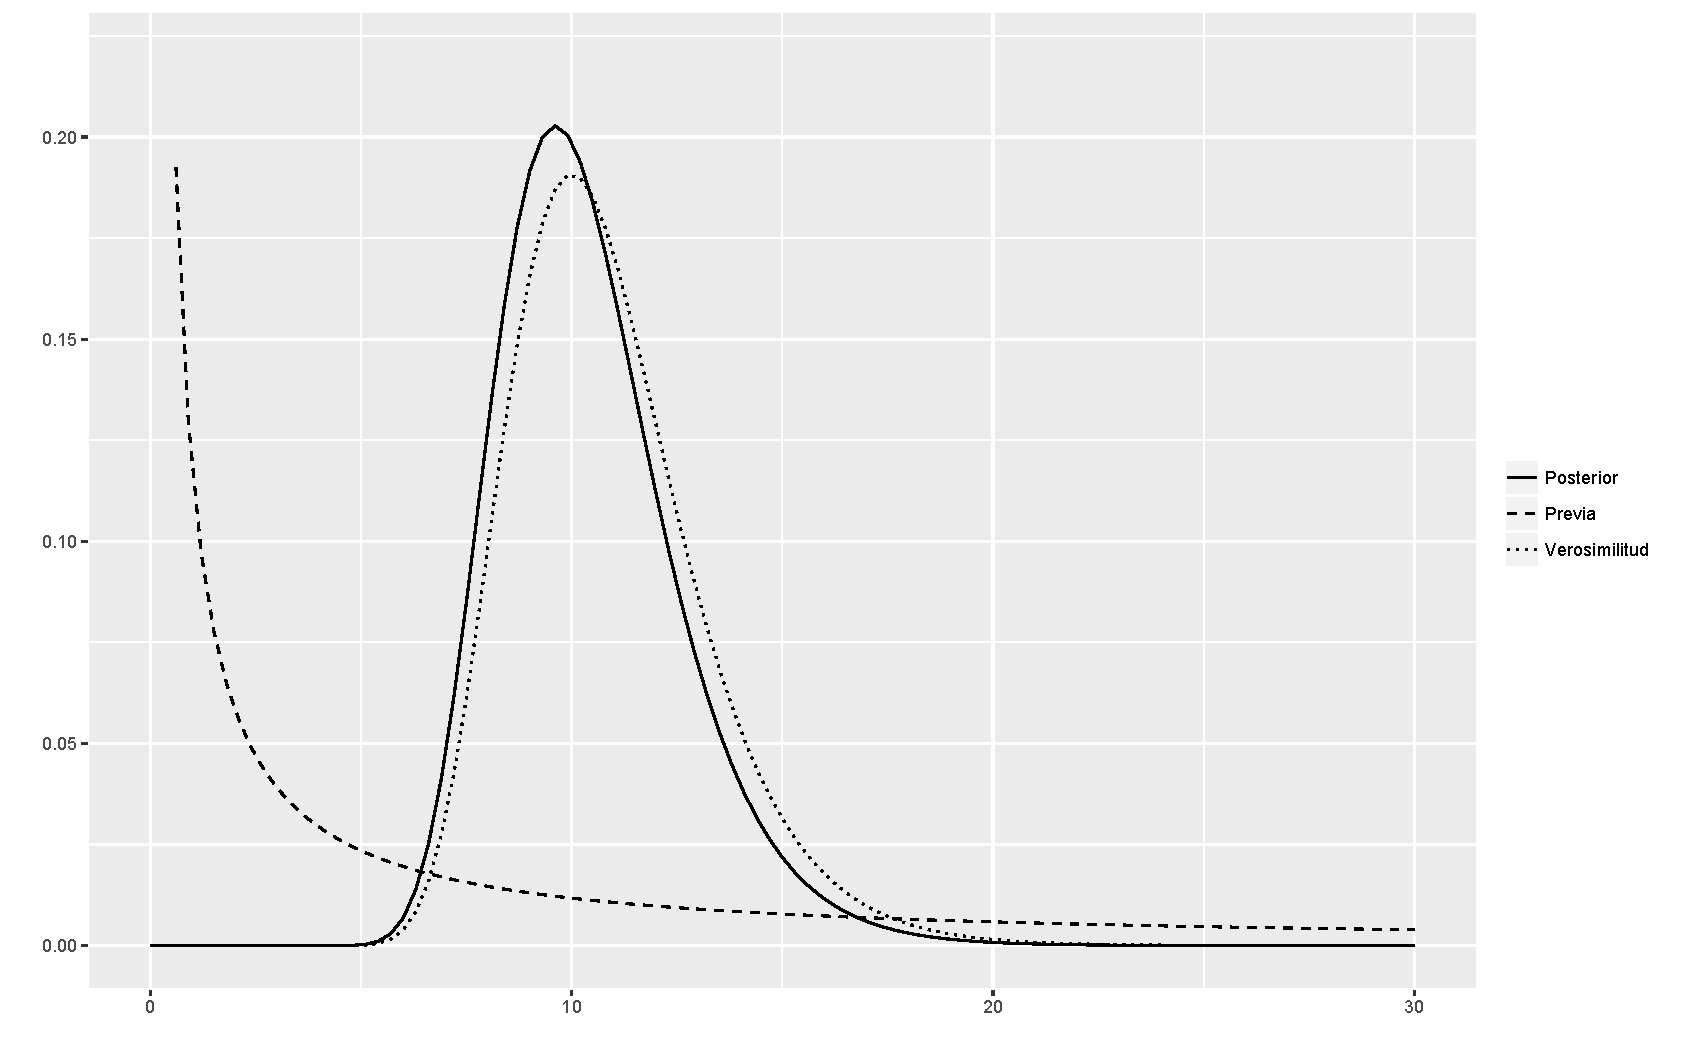
\includegraphics[scale=0.4]{Sigma2_Jeffreys.pdf}
    \caption{\emph{Distribuci\'on previa no informativa de Jeffreys, funci\'on de verosimilitud y distribuci\'on posterior de $\sigma^2$ con $n=50$ y $\hat{\sigma}^2_C=10$.}}
    \label{Posterior_Sigma2_Jeffreys}
    \end{figure}
    
Ahora, nos enfocamos en la distribuci\'on predictiva posterior para una nueva observaci\'on $\tilde{y}$ cuya expresi\'on se muestra en el siguiente resultado.
    \begin{Res}\label{pred_yy_sigma2}
    La distribuci\'on predictiva posterior de una nueva observaci\'on $\tilde{y}$, cuando se utiliza una distribuci\'on previa informativa para $\sigma^2$, es la distribuci\'on $t$ no estandarizado con grado de libertad $n_0+n$, el par\'ametro de localizaci\'on $\theta$ y el par\'ametro de escala $v_0/(n_0+n)$, donde $v_0=n_0\sigma^2_0+\sum_{i=1}^n(y_i-\theta)^2$, esto es, 
    \begin{equation*}
    \tilde{y} \mid \mathbf{Y}\sim t_{n_0+n}\left(\theta,\frac{v_0}{n_0+n}\right).
    \end{equation*} 
    
    Cuando se utiliza la distribuci\'on previa no informativa de Jeffreys para $\sigma^2$, la distrubci\'on predictiva de una nueva observaci\'on $\tilde{y}$ es $t_n(\theta,\hat{\sigma}^2_C)$, con $\hat{\sigma}^2_C=\frac{1}{n}\sum_{i=1}^n(y_i-\theta)^2$. 
    \end{Res}
    
    \begin{proof}
    Cuando la distribuci\'on previa para $\sigma^2$ es $Inversa-Gamma(n_0/2,\ n_0\sigma^2_0/2)$, la distribuci\'on posterior de $\sigma^2$ es $Inversa-Gamma((n_0+n)/2,\ (n_0\sigma^2_0+n\hat{\sigma}^2_C)/2)$, tenemos que 
    \begin{align*}
    p(\tilde{y}\mid\mathbf{Y})&=\int_0^\infty p(\tilde{y}\mid\sigma^2)p(\sigma^2\mid\mathbf{Y})\ d\sigma^2\\
    &=\int_0^\infty (2\pi\sigma^2)^{-1/2}\exp\left\{-\dfrac{1}{2\sigma^2}(\tilde{y}-\theta)^2\right\}\dfrac{(\frac{v_0}{2})^{(n_0+n)/2}(\sigma^2)^{-(n_0+n)/2-1}}{\Gamma(\frac{n_0+n}{2})}\exp\left\{-\dfrac{v_0}{2\sigma^2}\right\}\ d\sigma^2\\
    &=\dfrac{(2\pi)^{-1/2}(\frac{v_0}{2})^{(n_0+n)/2}}{\Gamma(\frac{n_0+n}{2})}\int_0^\infty(\sigma^2)^{-\frac{n_0+n+1}{2}-1}\exp\left\{-\dfrac{1}{\sigma^2}\left[\dfrac{v_0}{2}+\dfrac{1}{2}(\tilde{y}-\theta)^2\right]\right\}\ d\sigma^2\\
    &=\dfrac{(2\pi)^{-1/2}\Gamma(\frac{n_0+n+1}{2})}{\Gamma(\frac{n_0+n}{2})}\left(\frac{v_0}{2}\right)^{(n_0+n)/2}
    \left(\frac{v_0}{2}+\frac{1}{2}(\tilde{y}-\theta)^2\right)^{-\frac{n_0+n+1}{2}}\\
    &=\dfrac{(2\pi)^{-1/2}\Gamma(\frac{n_0+n+1}{2})}{\Gamma(\frac{n_0+n}{2})}\left(\frac{v_0}{2}\right)^{(n_0+n)/2}\left(\frac{v_0}{2}\right)^{-(n_0+n+1)/2}\left(1+\frac{(\tilde{y}-\theta)^2}{v_0}\right)^{-(n_0+n+1)/2}\\
    &=\dfrac{(2\pi)^{-1/2}\Gamma(\frac{n_0+n+1}{2})}{\Gamma(\frac{n_0+n}{2})}\left(\frac{v_0}{2}\right)^{-1/2}\left(1+\frac{(\tilde{y}-\theta)^2}{v_0}\right)^{-(n_0+n+1)/2}\\
    &=\dfrac{(\pi v_0)^{-1/2}\Gamma(\frac{n_0+n+1}{2})}{\Gamma(\frac{n_0+n}{2})}\left(1+\frac{(\tilde{y}-\theta)^2}{v_0}\right)^{-(n_0+n+1)/2}
    \end{align*}
    la cual corresponde a la funci\'on de densidad de la distribuci\'on $t_{n_0+n}\left(\theta,\frac{v_0}{n_0+n}\right)$. La distribuci\'on predictiva cuando se se usa la distribuci\'on previa de Jeffreys para $\sigma^2$ se deja como ejercicio (Ejercicio \ref{pre_y_sigma2_Jeffreys}).
    \end{proof}
    
    Del anterior resultado, tenemos que
    \begin{align*}
    E(\tilde{Y}\mid\mathbf{Y})&=\theta\\
    Var(\tilde{Y}\mid\mathbf{Y})&=\dfrac{v_0}{n_0+n}\dfrac{n_0+n}{n_0+n-2}=\dfrac{n_0\sigma^2_0+n\hat{\sigma}^2_C}{n_0+n-2}\\
    \end{align*}
    
    Podemos ver que la esperanza de la nueva observaci\'on es $\theta$, al igual que las variables de la muestra observada; mientras que la varianza de la nueva observaci\'on viene siendo aproximadamente un promedio ponderado entre la estimaci\'on previa de la varianza $\sigma^2_0$ y la estimaci\'on cl\'asica $\hat{\sigma}^2_C$, los pesos dependen de los tama\~nos de las dos fuentes de informaci\'on: $n_0$ y $n$. 
    
    Una forma alterna para aproximar el comportamiento aleatorio de $\tilde{Y}$ es usando la simulaci\'on. Se simulan valores de $\sigma^2$ desde su distribuci\'on posterior, y luego se simulan valores de $\tilde{Y}$ desde $p(\tilde{Y}\mid\sigma^2)$, es decir, de la distribuci\'on $Normal(\theta,\sigma^2)$. En la figura \ref{Simu_Y_pred1} se observa el histograma de 10 mil valores de $\tilde{Y}$ simulados con este procedimiento, en la misma gr\'afica se observa la funci\'on de densidad de la distribuci\'on predictiva de $\tilde{Y}$. Podemos que los valores obtenidos de esta forma concide plenamente con la distribuci\'on objetiva.
    
    \begin{figure}[!htb]\label{Simu_Y_pred1}
    \centering
    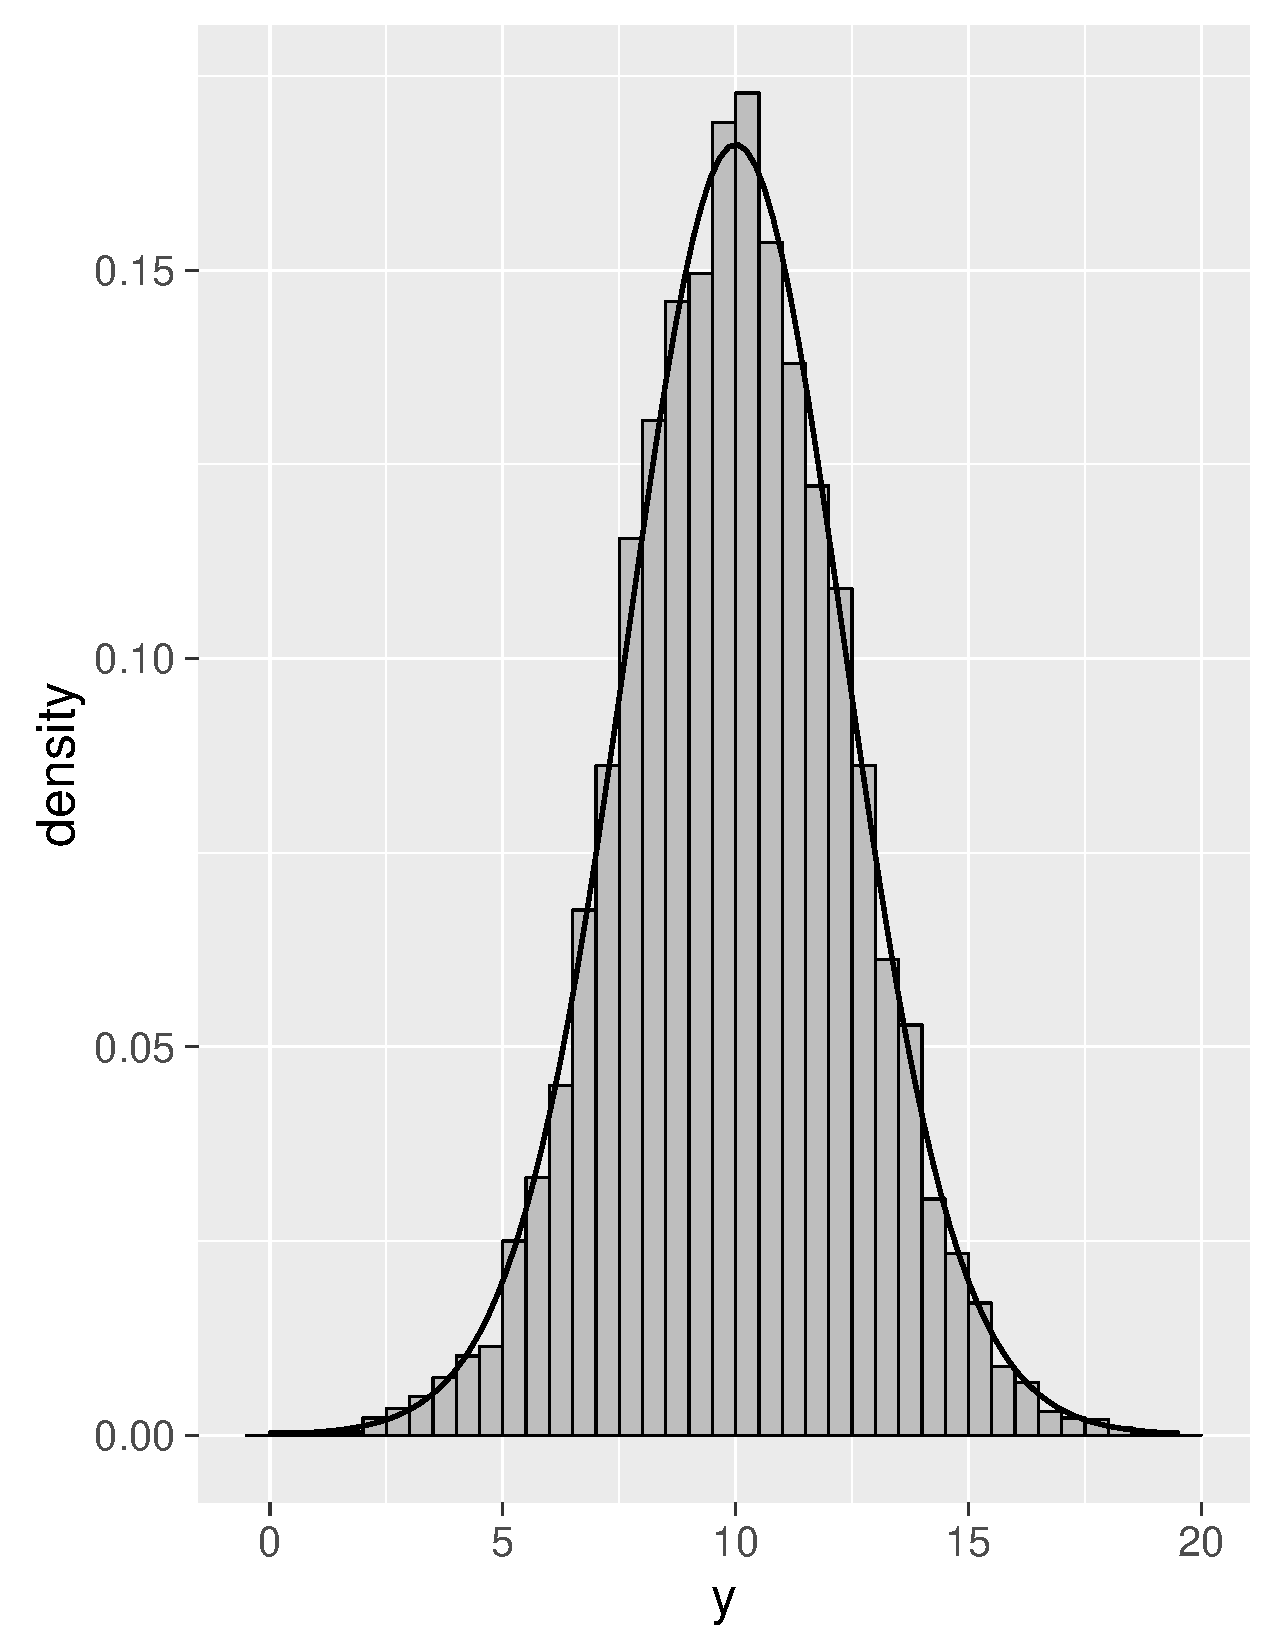
\includegraphics[scale=0.5,width=10cm,height=8cm]{Simu_Y_pred.pdf}
    \caption{\emph{Histograma de 10 mil valores simulados de $\tilde{y}$ y la funci\'on de densidad de la distribuci\'on predictiva $t_{n_0+n}(\theta,\frac{v_0}{n_0+n})$.}}
    \end{figure}
    
    Cuando es de inter\'es conocer el comportamiento de nuevas variables aleatorias $Y_1^*,\cdots,Y_{n^*}^*$, podemos obtener la distribuci\'on predictiva del valor promedio de estas nuevas medicicones: $\bar{Y}^*$. Esta distribuci\'on se encuenta en el siguiente resultado.
    
    \begin{Res}\label{pred_barY_sigma2}
    La distribuci\'on predictiva posterior de la media $\bar{Y}^* $ en una nueva muestrea $Y_1^*,\cdots,Y_{n^*}^*$, cuando se utiliza una distribuci\'on previa informativa para $\sigma^2$, es la distribuci\'on $t$ no estandarizado con grado de libertad $n_0+n$, el par\'ametro de localizaci\'on $\theta$ y el par\'ametro de escala $\frac{v_0}{n^*(n_0+n)}$, donde $v_0=n_0\sigma^2_0+\sum_{i=1}^n(y_i-\theta)^2$, esto es, 
    \begin{equation*}
    \bar{Y}^* \mid \mathbf{Y}\sim t_{n_0+n}\left(\theta,\frac{v_0}{n^*(n_0+n)}\right).
    \end{equation*} 
    
    Cuando se utiliza la distribuci\'on previa no informativa de Jeffreys para $\sigma^2$, la distrubci\'on predictiva de una nueva observaci\'on $\bar{Y}^*$ es
    
    \begin{equation*}
    \bar{Y}^* \mid \mathbf{Y}\sim t_n\left(\theta,\frac{\hat{\sigma}^2_C}{n^*}\right)
    \end{equation*} 
    con $\hat{\sigma}^2_C=\frac{1}{n}\sum_{i=1}^n(y_i-\theta)^2$. 
    \end{Res}
    
    \begin{proof}
    La demostraci\'on del resultado es similar a la del resultado \ref{pred_yy_sigma2}, y se deja como ejercicio para los lectores.
    \end{proof}
    
    \begin{Eje}
    Retomamos los datos usados en el ejemplo \ref{eje_vidrios} donde se cuenta con las siguientes 12 mediciones a l\'aminas de vidrios templados 3.56cm, 3.36cm, 2.99cm, 2.71cm, 3.31cm, 3.68cm, 2.78cm, 2.95cm, 2.82cm, 3.45cm, 3.42cm y 3.15cm. Los resultados inferenciales del ejemplo dejan entrever que el grosor promedio de las l\'aminas de esta l\'inea de producci\'on se puede asumir de 3cm, y queremos conocer un poco acerca de la varianza $\sigma^2$ de esta l\'inea de producci\'on, ya que un valor grande de $\sigma^2$ no es deseable ya que los productos ser\'ia muy ``disparejos'' entre ellos, y representa una falla para el proceso industrial. 
    
    Al asumir la media conocida $\theta=3cm$, se tiene que la estimaci\'on cl\'asica de $\sigma^2$ viene dada por $\hat{\sigma}^2_C=0.13cm^2$. Al utilizar la distribuci\'on previa no informativa de Jeffreys, la estimaci\'on bayesiana de $\sigma^2$ viene dada por $\frac{n}{n-2}\hat{\sigma}^2_C=0.157cm^2$. Para calcular un intervalo de credibilidad de 95\%, podemos usar el siguiente c\'odigo
\begin{knitrout}
\definecolor{shadecolor}{rgb}{0.933, 0.933, 0.933}\color{fgcolor}\begin{kframe}
\begin{alltt}
\hlkwd{library}\hlstd{(pscl)}
\hlkwd{qigamma}\hlstd{(}\hlnum{0.025}\hlstd{,} \hlkwc{alpha}\hlstd{=}\hlnum{12}\hlopt{/}\hlnum{2}\hlstd{,} \hlkwc{beta}\hlstd{=}\hlnum{12}\hlopt{*}\hlnum{0.13}\hlopt{/}\hlnum{2}\hlstd{)}
\end{alltt}
\begin{verbatim}
## [1] 0.06685
\end{verbatim}
\begin{alltt}
\hlkwd{qigamma}\hlstd{(}\hlnum{0.975}\hlstd{,} \hlkwc{alpha}\hlstd{=}\hlnum{12}\hlopt{/}\hlnum{2}\hlstd{,} \hlkwc{beta}\hlstd{=}\hlnum{12}\hlopt{*}\hlnum{0.13}\hlopt{/}\hlnum{2}\hlstd{)}
\end{alltt}
\begin{verbatim}
## [1] 0.3542
\end{verbatim}
\end{kframe}
\end{knitrout}
    
    de donde el intervalo para $\sigma^2$ est\'a dada por $(0.0668cm^2,0.3542cm^2)$. Para facilitar la interpretaci\'on de la estimaci\'on, es preferible estimar la desviaci\'on est\'andar $\sigma$. La estimaci\'on bayesiana de este par\'ametro ser\'ia $\hat{\sigma}_B=\sqrt{0.157cm^2}\approx 0.4cm$, y un intervalo de credibilidad para $\sigma$ viene dada por $(\sqrt{0.0668cm^2},\sqrt{0.3542cm^2})=(0.25cm,0.59cm)$.
    
    A continuaci\'on se ilustra el uso de \verb'JAGS' para obtener la estimaci\'on bayesiana del par\'ametro $\sigma^2$. En \verb'JAGS' no se admite el comando \verb'dflat()' para especificar una previa no informativa como lo hace \verb'WinBugs', por cual se debe definir la distribuci\'on previa escogiendo los par\'ametros que representa la falta de informaci\'on previa; por otro lado, se acostumbra a usar la distribuci\'on Gamma como la distribuci\'on previa del par\'ametro de precisi\'on $\tau=1/\sigma^2$, tal como se muestra a continuaci\'on.
    
\begin{knitrout}
\definecolor{shadecolor}{rgb}{0.933, 0.933, 0.933}\color{fgcolor}\begin{kframe}
\begin{alltt}
\hlstd{IG.model} \hlkwb{<-} \hlkwa{function}\hlstd{()\{}
\hlkwa{for}\hlstd{(i} \hlkwa{in} \hlnum{1} \hlopt{:} \hlstd{n)}
\hlstd{\{}
   \hlstd{y[i]} \hlopt{~} \hlkwd{dnorm}\hlstd{(}\hlnum{3}\hlstd{, tau)}
\hlstd{\}}
  \hlstd{sigma} \hlkwb{<-} \hlnum{1}\hlopt{/}\hlkwd{sqrt}\hlstd{(tau)}
  \hlstd{tau} \hlopt{~} \hlkwd{dgamma}\hlstd{(}\hlnum{0.001}\hlstd{,} \hlnum{0.001}\hlstd{)}
\hlstd{\}}

\hlstd{n} \hlkwb{<-} \hlnum{12}
\hlstd{y} \hlkwb{<-} \hlkwd{c}\hlstd{(}\hlnum{3.56}\hlstd{,} \hlnum{3.36}\hlstd{,} \hlnum{2.99}\hlstd{,} \hlnum{2.71}\hlstd{,} \hlnum{3.31}\hlstd{,} \hlnum{3.68}\hlstd{,} \hlnum{2.78}\hlstd{,} \hlnum{2.95}\hlstd{,} \hlnum{2.82}\hlstd{,} \hlnum{3.45}\hlstd{,} \hlnum{3.42}\hlstd{,} \hlnum{3.15}\hlstd{)}

\hlstd{IG.data} \hlkwb{<-} \hlkwd{list}\hlstd{(}\hlstr{"y"}\hlstd{,}\hlstr{"n"}\hlstd{)}
\hlstd{IG.param} \hlkwb{<-} \hlkwd{c}\hlstd{(}\hlstr{"sigma"}\hlstd{)}
\hlstd{IG.inits} \hlkwb{<-} \hlkwa{function}\hlstd{()\{}
  \hlkwd{list}\hlstd{(}\hlstr{"tau"}\hlstd{=}\hlkwd{c}\hlstd{(}\hlnum{1}\hlstd{))}
\hlstd{\}}

\hlstd{IG.fit} \hlkwb{<-} \hlkwd{jags}\hlstd{(}\hlkwc{data}\hlstd{=IG.data,} \hlkwc{inits}\hlstd{=IG.inits, IG.param,} \hlkwc{n.iter}\hlstd{=}\hlnum{10000}\hlstd{,}
    \hlkwc{n.burnin}\hlstd{=}\hlnum{1000}\hlstd{,} \hlkwc{model.file}\hlstd{=IG.model)}

\hlkwd{print}\hlstd{(IG.fit)}
\end{alltt}
\end{kframe}
\end{knitrout}
    
    De los anteriores c\'odigos, se obtiene que la estimaci\'on bayesiana resultante para $\sigma$ es de 0.388cm, con un intervalo de credibilidad del 95\% de $(0.258cm,0.605cm)$, resultados muy similares a lo presentado anteriormente. 
\end{Eje}

\section{Ejercicios}
\begin{enumerate}
\item En una muestra aleatoria de variables con distribuci\'on $Exponencial$ con param\'emetro $\theta$, verifique que la distribuci\'on previa no informativa de Jeffreys est\'a dada por
\begin{equation}
p(\theta)\propto \theta^{-1}
\end{equation}
\item\label{XXX} Desarrolla los c\'alculos necesarios para comprobar que para datos normales con varianza conocida, la distribuci\'on posterior de la media $\theta$ es $Normal(\bar{y},\sigma^2/n)$ cuando la distribuci\'on previa es $p(\theta)\propto cte$. 
\item Demuestre el resultado \ref{pred_y_theta}.
\item\label{Ejer_pre_Jeffreys} Demuestre la segunda parte del resultado \ref{pred_norm}.
\item Demuestre que en datos con distribuci\'on normal: $Y_1,\cdots,Y_n\sim N(\theta,\sigma^2)$ con $\theta$ conocido, al utilizar la distribuci\'on previa no informativa de Jeffreys para $\sigma^2$, la distrubci\'on de posterior de $\sigma^2$ viene dada por $Inversa-Gamma(\frac{n}{2},\frac{n\hat{\sigma}^2_C}{2})$ con $\hat{\sigma}^2_C=\frac{1}{n}\sum_{i=1}^n(y_i-\theta)^2$. 
\item\label{pre_y_sigma2_Jeffreys} Demuestre que en datos con distribuci\'on normal: $Y_1,\cdots,Y_n\sim N(\theta,\sigma^2)$ con $\theta$ conocido, al utilizar la distribuci\'on previa no informativa de Jeffreys para $\sigma^2$, la distrubci\'on predictiva de una nueva observaci\'on $\tilde{y}$ es $t_n(\theta,\hat{\sigma}^2_C)$, con $\hat{\sigma}^2_C=\frac{1}{n}\sum_{i=1}^n(y_i-\theta)^2$. 
\item Demuestre el resultado \ref{pred_barY_sigma2}.
\end{enumerate}



    


%--------------------
 
\chapter{Modelos multiparam\'etricos}
En este cap\'itulo, discutimos situaciones donde se requieren estimar simult\'aneamente m\'as de un par\'ametro, es decir, los datos que enfrentamos se ajustan a una distrubuci\'on de probabilidad que involucre a multiples par\'ametros. Espec\'ificamente, se estudiar\'a las siguientes distribuciones

\begin{itemize}
\item La distribuci\'on normal univariada que tiene dos par\'ametros: la media $\theta$ y la varianza $\sigma^2$,
\item La distribuci\'on normal mutivariada con vector de medias $\btheta$ y la matriz de varianzas y covarianzas $\bSigma$, y
\item La distribuci\'on multinomial cuyo par\'ametro constituye en el vector de probabilidades $\btheta$.
\end{itemize}

En el contexto de la estimaci\'on bayesiana, es necesario hallar la distribuci\'on posterior conjunta de estos par\'ametros, y encontrar la estimaci\'on por alguna de las siguientes dos formas: (1) hallar te\'oricamente la esperanza de la distribuci\'on posterior conjunta, \'o (2) simular valores de la distribuci\'on posterior conjunta, de donde se puede obtener la estimaci\'on puntual y por intervalo.

\section{Normal univariada con media y varianza desconocida}

Supongamos que se dispone de realizaciones de un conjunto de variables independientes e id\'enticamente distribuidos $Y_1,\cdots,Y_n\sim N(\theta,\sigma^2)$, cuando se desconoce tanto la media como la varianza de la distribuci\'on, es necesario plantear diversos enfoques y situarse en el m\'as conveniente, seg\'un el contexto del problema. En t\'erminos de la asignaci\'on de las distribuciones previa para $\theta$ y $\sigma^2$ es posible:
\begin{itemize}
\item Suponer que la distribuci\'on previa $p(\theta)$ es independiente de la distribuci\'on previa $p(\sigma^2)$ y que ambas distribuciones son informativas. 
\item Suponer que la distribuci\'on previa $p(\theta)$ es independiente de la distribuci\'on previa $p(\sigma^2)$ y que ambas distribuciones son no informativas.
\item Suponer que la distribuci\'on previa para $\theta$ depende de $\sigma^2$ y escribirla como $p(\theta \mid \sigma^2)$, mientras que la distribuci\'on previa de $\sigma^2$ no depende de $\theta$ y se puede escribir como $p(\sigma^2)$.
\end{itemize}

A continuaci\'on, analizamos cada uno de estos planteamientos, y desarrollamos los resultados necesrios para la estimaci\'on de $\theta$ y $\sigma^2$.

\subsection{Par\'ametros independientes}

El primer enfoque que considermos para el an\'alisis de los par\'ametros de inter\'es $\theta$ y $\sigma^2$ en una distribuci\'on normal univariada es suponer que las distribuciones previa de cada uno de los par\'ametros son independientes pero al mismo tiempo son informativas. \citeasnoun{Gelman03} afirma que este supuesto de independencia es atractivo en problemas para los cuales la informaci\'on previa para $\theta$ no toma la forma de un n\'umero fijo de observaciones con varianza $\sigma^2$. Adicionalmente, este supuesto de independencia es coeherente con el hecho de que en la teor\'ia cl\'asica de estimaci\'on los estimadores insesgados de varianza m\'inima de $\theta$ y $\sigma^2$ son independientes (ver \citeasnoun[Sec.2.4]{Zhang}).

En este orden de ideas, y siguiendo la argumentaci\'on del cap\'itulo anterior, la distribuci\'on previa para el par\'ametro $\theta$ es
\begin{equation*}
\theta \sim Normal(\mu,\tau^2)
\end{equation*}


y la distribuci\'on previa para el par\'ametro $\sigma^2$ es
\begin{equation*}
\sigma^2 \sim Inversa-Gamma(n_0/2,n_0\sigma^2_0/2)
\end{equation*}

Asumiendo independencia previa, la distribuci\'on previa conjunta est\'a dada por
\begin{equation}
p(\theta,\sigma^2)\propto (\sigma^2)^{-n_0/2-1}\exp\left\{-\dfrac{n_0\sigma^2_0}{2\sigma^2}\right\}
\exp\left\{-\frac{1}{2\tau^2}(\theta-\mu)^2\right\}
\end{equation}

Una vez que se conoce la forma estructural de la distribuci\'on previa conjunta, es posible establecer la distribuci\'on posterior conjunta puesto que la verosimilitud de los datos, $p(\mathbf{Y} \mid \theta,\sigma^2)$, est\'a dada por la expresi\'on (\ref{vero_normal}) y
\begin{equation*}
p(\theta,\sigma^2 \mid \mathbf{Y})\propto p(\mathbf{Y} \mid \theta,\sigma^2)p(\theta,\sigma^2)
\end{equation*}

\begin{Res}
La distribuci\'on posterior conjunta de los par\'ametros de inter\'es est\'a dada por
\begin{align}
p(\theta,\sigma^2 \mid \mathbf{Y})&\propto (\sigma^2)^{-(n+n_0)/2-1} \notag \\
&\times
\exp\left\{-\frac{1}{2\sigma^2}\left[n_0\sigma^2_0+(n-1)S^2
                                     +n(\bar{y}-\theta)^2\right]-\frac{1}{2\tau^2}(\theta-\mu)^2\right\}
\end{align}
\end{Res}


\begin{proof}
Tenemos que
\begin{align*}
p(\theta,\sigma^2 \mid \mathbf{Y})&\propto p(\mathbf{Y} \mid \theta,\sigma^2)p(\theta,\sigma^2)\\
&\propto(\sigma^2)^{-n/2}\exp\left\{-\frac{1}{2\sigma^2}\sum_{i=1}^n(y_i-\theta)^2\right\}(\sigma^2)^{-n_0/2-1}\exp\left\{-\dfrac{n_0\sigma^2_0}{2\sigma^2}\right\}
\exp\left\{-\frac{1}{2\tau^2}(\theta-\mu)^2\right\} \\
&=(\sigma^2)^{-(n+n_0)/2-1}\exp\left\{-\frac{1}{2\sigma^2}\left[n_0\sigma^2_0+\sum_{i=1}^n(y_i-\theta)^2\right]-\frac{1}{2\tau^2}(\theta-\mu)^2\right\}\\
&\propto (\sigma^2)^{-(n+n_0)/2-1}\exp\left\{-\frac{1}{2\sigma^2}\left[n_0\sigma^2_0+(n-1)S^2
                                     +n(\bar{y}-\theta)^2\right]-\frac{1}{2\tau^2}(\theta-\mu)^2\right\}
\end{align*}
dond la \'ultima expresi\'on se obtiene al sumar y restar $\bar{y}$ dentro de $(y_i-\theta)^2$.
\end{proof}


N\'otese que la distribuci\'on posterior conjunta no tiene una forma estructural conocida y por lo tanto no es posible realizar el m\'etodo de integraci\'on anal\'itica para obtener una constante de integraci\'on \cite{Migon}. Sin embargo, s\'i es posible obtener las distribuciones condicionales posterior de $\theta$ y de $\sigma^2$, notando que
\begin{align*}
p(\theta \mid \sigma^2,\mathbf{Y})\propto p(\theta,\underbrace{\sigma^2}_{fijo} \mid \mathbf{Y})
\ \ \ \ \ \ \ \ \ \text{y} \ \ \ \ \ \ \ \ \ \
p(\sigma^2 \mid \theta,\mathbf{Y})\propto p(\underbrace{\theta}_{fijo},\sigma^2 \mid \mathbf{Y})
\end{align*}

Es decir, para encontrar la distribuci\'on posterior marginal de $\theta$ dado $\sigma^2$, se utiliza la distribuci\'on posterior conjunta y los t\'erminos que no dependan de $\theta$ se incorporan en la constante de proporcionalidad. El mismo razonamiento se aplica para el par\'ametro $\sigma^2$.

\begin{Res}
La distribuci\'on posterior condicional de $\theta$ es
\begin{equation}\label{Post_theta_Gibbs}
\theta  \mid  \sigma^2,\mathbf{Y} \sim Normal(\mu_n,\tau_n^2)
\end{equation}
En donde las expresiones para $\mu_n$ y $\tau_n^2$ est\'an dadas por \ref{tau_sigma_n}. Por otro lado, la distribuci\'on posterior condicional de $\sigma^2$ es 
\begin{equation}\label{Post_Sigma2_Gibbs}
\sigma^2  \mid  \theta,\mathbf{Y} \sim Inversa-Gamma\left(\dfrac{n_0+n}{2},\dfrac{v_0}{2}\right)
\end{equation}
con $v_0=n_0\sigma^2_0+(n-1)S^2+n(\bar{y}-\theta)^2$.
\end{Res}

\begin{proof}
Acudiendo a la distribuci\'on posterior conjunta e incorporando los t\'erminos que no dependen de $\theta$ en la constante de proporcionalidad, se tiene que
\begin{align*}
p(\theta \mid \sigma^2,\mathbf{Y})&\propto \exp\left\{-\frac{n}{2\sigma^2}(\bar{y}-\theta)^2-\frac{1}{2\tau^2}(\theta-\mu)^2\right\}
\end{align*}
Completando los cuadrados y siguiendo el razonamiento de la demostraci\'on del resultado \ref{Res_pos_theta}, se encuentra una expresi\'on id\'entica a la funci\'on de distribuci\'on de una variable aleatoria con distribuci\'on $Normal(\mu_n, \tau^2_n)$. Para la distribuci\'on posterior condicional de $\sigma^2$, consultar el resultado \ref{posterior_sigma2}.
\end{proof}

Una vez encontradas las distribuciones posteriores condicionales de $\theta$ y $\sigma^2$, se puede obtener la estimaci\'on de estos par\'ametros usando m\'etodos de Monte Carlo, espec\'ificamente el muestreo de Gibbs, que puesto en el contexto de este cap\'itulo, se resume en los siguientes pasos:
\begin{enumerate}[(1)]
\item Fijar un valor inicial para $\theta$, lo denotamos por $\theta_{(1)}$
\item Simular un valor de la distribuci\'on de $\sigma^2|\theta,\mathbf{Y}$ en (\ref{Post_Sigma2_Gibbs}) donde el par\'ametro $v_0$ que depende de $\theta$, debe ser reemplazado por $\theta_{(1)}$ del paso anterior. Este valor simulado se denotar\'a por $\sigma^2_{(1)}$
\item  Simlar un valor de la distribuci\'on de $\theta|\sigma^2,\mathbf{Y}$ en (\ref{Post_theta_Gibbs}) donde en $\mu_n$ y $\tau^2_n$ se debe reemplazar $\sigma^2$ por $\sigma^2_{(1)}$. Este valor simulado se denota por $\theta_{(2)}$.
\item Se repite los pasos (2) y (3) hasta completar un n\'umero de iteraciones suficientes para alcanzar la convergencia en ambos par\'ametros
\end{enumerate}

Despu\'es de ejecutar el muestreador de Gibbs, se eliminan los primeros valores simulados para descartar influencia del valor inicial y posiblemente se deba efectuar el \emph{thinning} para eliminar correlaciones que pueden estar presentes. Posterior a eso, tenemos los valores finales simulados de $\theta$ y $\sigma^2$, de donde podemos calcular la estimaci\'on tomando los promedios respectivos, y calcular intervalos de credibilidad como los percentiles muestrales de los valores simulados. 

En cuanto a la distribuci\'on predictiva para una nueva observaci\'on $\tilde{y}$, esta est\'a dada por
\begin{equation*}
p(\tilde{y}\mid\mathbf{Y})=\int_0^\infty\int_{-\infty}^\infty p(\tilde{y}\mid\theta,\ \sigma^2)p(\theta,\ \sigma^2\mid\mathbf{Y})d\theta\ d\sigma^2
\end{equation*}

Hallar esta distribuci\'on de forma exacta no es f\'acil, y podemos optar por conocer el comportamiento probabil\'istico de $\tilde{y}$ por medio de la simulaci\'on. Tal como se explic\'o en el cap\'itulo anterior, se debe simular en primer lugar valores de $\theta$ y de $\sigma^2$ de la distribuci\'on posterior $p(\theta,\ \sigma^2\mid\mathbf{Y})$ usando el muestreador de Gibbs y posteriormente se simula valores de $\tilde{y}$ de la distribuci\'on $p(\tilde{y}\mid\theta,\ \sigma^2)$. 

Ahora, si se quiere conocer el comportamiento de una nueva muestra aleatoria $Y_1^{*},\cdots,Y_{n^*}^{*}$, lo podemos hacer por medio de la distribuci\'on predictiva de la media $\bar{Y}^*$ de la siguiente forma: se debe simular en primer lugar valores de $\theta$ y de $\sigma^2$ de la distribuci\'on posterior $p(\theta,\ \sigma^2\mid\mathbf{Y})$ usando el muestreador de Gibbs y posteriormente se simula valores de $\bar{Y}^*$ de la distribuci\'on $N(\theta,\frac{\sigma^2}{n^*})$.


\begin{Eje}\label{Eje-Renal}
\citeasnoun{Efronims} consider\'o un conjunto de datos que muestran la funci\'on renal de 157 individuos que se sometieron a una prueba m\'edica exhaustiva en un hospital. Los resultados de la prueba renal est\'an en un intervalo de -6 puntos a 4 puntos. Entre m\'as alto sea el resultado, se concluye que el ri\~n\'on del individuo es m\'as sano. N\'otese que estas pruebas son importantes para predecir el comportamiento de un ri\~n\'on donado a un paciente con problemas renales. Los datos son extra\'idos de la siguiente p\'agina WEB  (\url{http://statweb.stanford.edu/~ckirby/brad/LSI/datasets-and-programs/datasets.html}) y para este ejemplo s\'olo se utilizaron los primeros 15 datos del archivo.

En principio, es de inter\'es para el investigador conocer la media y la dispersi\'on de estos datos, para poder analizar a fondo la situaci\'on de los pacientes que esperan un transplante.

Dado que se trata de una primera aproximaci\'on, se prefiere utilizar distribuciones previas no informativas para los par\'ametros de la media y varianza. Lo anterior se logra en \verb'JAGS' definiendo las distribuciones previas de \verb"mu ~ dnorm(0,0.001)" y de \verb"tau ~ dgamma(0.001,0.001)" donde \verb"tau" corresponde al par\'ametro de precisi\'on que resulta ser el inverso de la varianza $\sigma^2$. De esta forma, la distribuci\'on previa de $mu$ est\'a centrada en cero, pero con una varianza muy grande al igual que la distribuci\'on de la varianza, los cuales representan distribuciones previas no informativas.

El siguiente c\'odigo en \verb'JAGS' muestra c\'omo se lleva a cabo la inferencia.
\begin{knitrout}
\definecolor{shadecolor}{rgb}{0.933, 0.933, 0.933}\color{fgcolor}\begin{kframe}
\begin{alltt}
\hlstd{Model} \hlkwb{<-} \hlkwa{function}\hlstd{()\{}
  \hlkwa{for} \hlstd{(i} \hlkwa{in} \hlnum{1}\hlopt{:}\hlstd{n)}
  \hlstd{\{}
    \hlstd{y[i]} \hlopt{~} \hlkwd{dnorm}\hlstd{(theta,tau)}
  \hlstd{\}}
  \hlstd{theta} \hlopt{~} \hlkwd{dnorm}\hlstd{(}\hlnum{0}\hlstd{,}\hlnum{0.001}\hlstd{);}
  \hlstd{sigma} \hlkwb{<-} \hlnum{1}\hlopt{/}\hlkwd{sqrt}\hlstd{(tau)}
  \hlstd{tau} \hlopt{~} \hlkwd{dgamma}\hlstd{(}\hlnum{0.001}\hlstd{,} \hlnum{0.001}\hlstd{)}
\hlstd{\}}

\hlstd{n} \hlkwb{<-} \hlnum{15}
\hlstd{y} \hlkwb{<-} \hlkwd{c}\hlstd{(}\hlnum{1.69045085}\hlstd{,} \hlopt{-}\hlnum{1.41076082}\hlstd{,} \hlopt{-}\hlnum{0.27909483}\hlstd{,} \hlopt{-}\hlnum{0.91387987}\hlstd{,} \hlnum{3.21868429}\hlstd{,} \hlopt{-}\hlnum{1.47282460}\hlstd{,}
       \hlopt{-}\hlnum{0.96524353}\hlstd{,} \hlopt{-}\hlnum{2.45084934}\hlstd{,} \hlnum{1.03838153}\hlstd{,} \hlnum{1.79928679}\hlstd{,} \hlnum{0.97826621}\hlstd{,} \hlnum{0.67463830}\hlstd{,}
       \hlopt{-}\hlnum{1.08665864}\hlstd{,} \hlopt{-}\hlnum{0.00509027}\hlstd{,} \hlnum{0.43708128}\hlstd{)}

\hlstd{Model.data} \hlkwb{<-} \hlkwd{list}\hlstd{(}\hlstr{"y"}\hlstd{,}\hlstr{"n"}\hlstd{)}
\hlstd{Model.param} \hlkwb{<-} \hlkwd{c}\hlstd{(}\hlstr{"theta"}\hlstd{,} \hlstr{"sigma"}\hlstd{)}
\hlstd{Model.inits} \hlkwb{<-} \hlkwa{function}\hlstd{()\{}
  \hlkwd{list}\hlstd{(}\hlstr{"theta"}\hlstd{=}\hlkwd{c}\hlstd{(}\hlnum{0}\hlstd{),} \hlstr{"tau"}\hlstd{=}\hlkwd{c}\hlstd{(}\hlnum{1}\hlstd{))}
\hlstd{\}}

\hlstd{Model.fit} \hlkwb{<-} \hlkwd{jags}\hlstd{(}\hlkwc{data}\hlstd{=Model.data,} \hlkwc{inits}\hlstd{=Model.inits, Model.param,} \hlkwc{n.iter}\hlstd{=}\hlnum{10000}\hlstd{,}
               \hlkwc{n.burnin}\hlstd{=}\hlnum{1000}\hlstd{,} \hlkwc{model.file}\hlstd{=Model)}

\hlkwd{print}\hlstd{(Model.fit)}
\end{alltt}
\end{kframe}
\end{knitrout}

Despu\'es de ejecutar diez mil iteraciones, la salida del anterior c\'odigo muestra una estimaci\'on puntual para la esperanza de $Y$ de 0.087 con un intervalo de credibilidad del 95\% dado por (-0.75, 0.95). Por otro lado, la estimaci\'on puntual de la desviaci\'on est\'andar de $Y$ es de 1.557 con un intervalo de credibilidad del 95\% dado por (1.12, 2.39).

A continuaci\'on se ilustra el uso de \verb'R' el algoritmo de Gibbs para los datos del ejemplo. Se recalca que se utiliza la librer\'ia \verb"MCMCpack" \cite{MCMCpack} para generar las realizaciones de la distribuci\'on Inversa-Gamma.

\begin{knitrout}
\definecolor{shadecolor}{rgb}{0.933, 0.933, 0.933}\color{fgcolor}\begin{kframe}
\begin{alltt}
\hlkwd{set.seed}\hlstd{(}\hlnum{123456}\hlstd{)}
\hlkwd{library}\hlstd{(MCMCpack)}
\end{alltt}


{\ttfamily\noindent\itshape\color{messagecolor}{\#\# Loading required package: MASS}}

{\ttfamily\noindent\itshape\color{messagecolor}{\#\# \#\#\\\#\# \#\# Markov Chain Monte Carlo Package (MCMCpack)}}

{\ttfamily\noindent\itshape\color{messagecolor}{\#\# \#\# Copyright (C) 2003-2018 Andrew D. Martin, Kevin M. Quinn, and Jong Hee Park}}

{\ttfamily\noindent\itshape\color{messagecolor}{\#\# \#\#\\\#\# \#\# Support provided by the U.S. National Science Foundation}}

{\ttfamily\noindent\itshape\color{messagecolor}{\#\# \#\# (Grants SES-0350646 and SES-0350613)\\\#\# \#\#}}\begin{alltt}
\hlstd{y} \hlkwb{<-} \hlkwd{c}\hlstd{(}\hlnum{1.69045085}\hlstd{,} \hlopt{-}\hlnum{1.41076082}\hlstd{,} \hlopt{-}\hlnum{0.27909483}\hlstd{,} \hlopt{-}\hlnum{0.91387987}\hlstd{,} \hlnum{3.21868429}\hlstd{,} \hlopt{-}\hlnum{1.47282460}\hlstd{,}
       \hlopt{-}\hlnum{0.96524353}\hlstd{,} \hlopt{-}\hlnum{2.45084934}\hlstd{,} \hlnum{1.03838153}\hlstd{,} \hlnum{1.79928679}\hlstd{,} \hlnum{0.97826621}\hlstd{,} \hlnum{0.67463830}\hlstd{,}
       \hlopt{-}\hlnum{1.08665864}\hlstd{,} \hlopt{-}\hlnum{0.00509027}\hlstd{,} \hlnum{0.43708128}\hlstd{)}

\hlstd{n} \hlkwb{<-} \hlkwd{length}\hlstd{(y)}

\hlcom{#parametros previos de theta}
\hlstd{mu} \hlkwb{<-} \hlnum{0}\hlstd{; tau2} \hlkwb{<-} \hlnum{1000}
\hlcom{#parametros previos de sigma2}
\hlstd{a} \hlkwb{<-} \hlnum{0.001}\hlstd{; b} \hlkwb{<-} \hlnum{0.001}

\hlstd{nsim} \hlkwb{<-} \hlnum{10000}
\hlstd{theta.pos} \hlkwb{<-} \hlkwd{rep}\hlstd{(}\hlnum{NA}\hlstd{,nsim)}
\hlstd{sigma2.pos} \hlkwb{<-} \hlkwd{rep}\hlstd{(}\hlnum{NA}\hlstd{,nsim)}

\hlcom{# Valor inicial de theta}
\hlstd{theta.pos[}\hlnum{1}\hlstd{]} \hlkwb{<-} \hlnum{0}

\hlcom{#parametros posteriores de sigma2	}
\hlstd{a.n} \hlkwb{<-} \hlstd{a}\hlopt{+}\hlstd{n}\hlopt{/}\hlnum{2}
\hlstd{b.n} \hlkwb{<-} \hlstd{b}\hlopt{+}\hlstd{((n}\hlopt{-}\hlnum{1}\hlstd{)}\hlopt{*}\hlkwd{var}\hlstd{(y)}\hlopt{+}\hlstd{n}\hlopt{*}\hlstd{(}\hlkwd{mean}\hlstd{(y)}\hlopt{-}\hlstd{theta.pos[}\hlnum{1}\hlstd{]))}\hlopt{/}\hlnum{2}
\hlcom{#simulacion de la distribucion posterior condicional de theta}
\hlstd{sigma2.pos[}\hlnum{1}\hlstd{]} \hlkwb{<-} \hlkwd{rinvgamma}\hlstd{(}\hlnum{1}\hlstd{, a.n, b.n)}
\hlcom{########################}
\hlcom{# Muestreador de Gibbs #}
\hlcom{########################}
\hlkwa{for}\hlstd{(i} \hlkwa{in} \hlnum{2}\hlopt{:}\hlstd{nsim)\{}
  \hlcom{#parametros posteriores de theta	}
  \hlstd{tau2.n} \hlkwb{<-} \hlnum{1} \hlopt{/} \hlstd{((n}\hlopt{/}\hlstd{sigma2.pos[i}\hlopt{-}\hlnum{1}\hlstd{])}\hlopt{+}\hlstd{(}\hlnum{1}\hlopt{/}\hlstd{tau2))}
  \hlstd{mu.n} \hlkwb{<-} \hlstd{tau2.n} \hlopt{*} \hlstd{(}\hlkwd{mean}\hlstd{(y)} \hlopt{*} \hlstd{(n}\hlopt{/}\hlstd{sigma2.pos[i}\hlopt{-}\hlnum{1}\hlstd{])}\hlopt{+}\hlstd{mu}\hlopt{/}\hlstd{tau2)}
  \hlcom{#simulacion de la distribucion posterior condicional de theta}
  \hlstd{theta.pos[i]} \hlkwb{<-} \hlkwd{rnorm}\hlstd{(}\hlnum{1}\hlstd{,} \hlkwc{mean}\hlstd{=mu.n,} \hlkwc{sd}\hlstd{=}\hlkwd{sqrt}\hlstd{(tau2.n))}
  \hlcom{#parametros posteriores de sigma2	}
  \hlstd{a.n} \hlkwb{<-} \hlstd{a} \hlopt{+} \hlstd{n}\hlopt{/}\hlnum{2}
  \hlstd{b.n} \hlkwb{<-} \hlstd{b} \hlopt{+} \hlstd{((n}\hlopt{-}\hlnum{1}\hlstd{)} \hlopt{*} \hlkwd{var}\hlstd{(y)} \hlopt{+} \hlstd{n} \hlopt{*} \hlstd{(}\hlkwd{mean}\hlstd{(y)}\hlopt{-}\hlstd{theta.pos[i]))} \hlopt{/} \hlnum{2}
  \hlcom{#simulacion de la distribucion posterior condicional de theta}
  \hlstd{sigma2.pos[i]} \hlkwb{<-} \hlkwd{rinvgamma}\hlstd{(}\hlnum{1}\hlstd{, a.n, b.n)}
\hlstd{\}}
\hlkwd{par}\hlstd{(}\hlkwc{mfrow}\hlstd{=}\hlkwd{c}\hlstd{(}\hlnum{1}\hlstd{,}\hlnum{2}\hlstd{))}
\hlkwd{acf}\hlstd{(theta.pos[}\hlnum{1001}\hlopt{:}\hlstd{nsim])}
\hlkwd{acf}\hlstd{(sigma2.pos[}\hlnum{1001}\hlopt{:}\hlstd{nsim])}
\end{alltt}
\end{kframe}
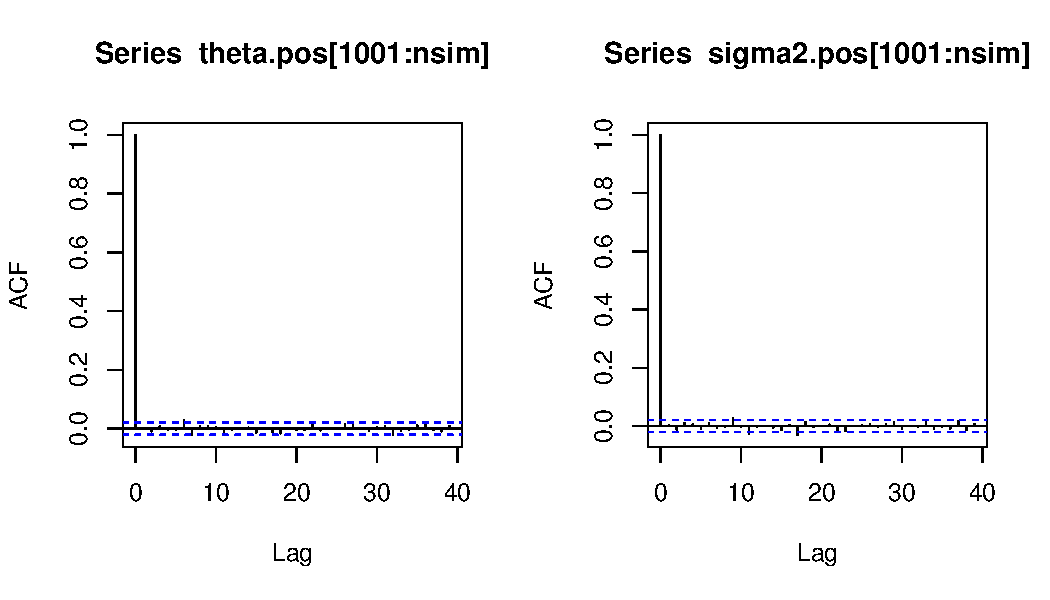
\includegraphics[width=\maxwidth]{figure/unnamed-chunk-34-1} 

\end{knitrout}
Al observar que no existen correlaciones importantes en los valores simulados de $\theta$ y $\sigma^2$ (despu\'es de descartar las primeras 1000 iteraciones), se concluye que se puede utilizar directamente estos valores para la obtenci\'on de las estimaciones. Por cual, se calcula el promedio y los percentiles muestrales de los valores simulados de la siguiente forma:
\begin{knitrout}
\definecolor{shadecolor}{rgb}{0.933, 0.933, 0.933}\color{fgcolor}\begin{kframe}
\begin{alltt}
\hlkwd{mean}\hlstd{(theta.pos[}\hlnum{1001}\hlopt{:}\hlstd{nsim])}
\end{alltt}
\begin{verbatim}
## [1] 0.08
\end{verbatim}
\begin{alltt}
\hlkwd{quantile}\hlstd{(theta.pos[}\hlnum{1001}\hlopt{:}\hlstd{nsim],} \hlkwd{c}\hlstd{(}\hlnum{0.025}\hlstd{,}\hlnum{0.975}\hlstd{))}
\end{alltt}
\begin{verbatim}
##  2.5%   98% 
## -0.72  0.90
\end{verbatim}
\begin{alltt}
\hlkwd{mean}\hlstd{(}\hlkwd{sqrt}\hlstd{(sigma2.pos[}\hlnum{1001}\hlopt{:}\hlstd{nsim]))}
\end{alltt}
\begin{verbatim}
## [1] 1.5
\end{verbatim}
\begin{alltt}
\hlkwd{quantile}\hlstd{(}\hlkwd{sqrt}\hlstd{(sigma2.pos[}\hlnum{1001}\hlopt{:}\hlstd{nsim]),} \hlkwd{c}\hlstd{(}\hlnum{0.025}\hlstd{,}\hlnum{0.975}\hlstd{))}
\end{alltt}
\begin{verbatim}
## 2.5%  98% 
##  1.0  2.3
\end{verbatim}
\end{kframe}
\end{knitrout}

De donde podemos concluir que una estimaci\'on puntual para la esperanza de $Y$ de 0.08 con un intervalo de credibilidad del 95\% dado por (-0.73, 0.89). Por otro lado, la estimaci\'on puntual de la desviaci\'on est\'andar de $Y$ es de 1.5 con un intervalo de credibilidad del 95\% dado por (1.0, 2.3), resultados muy similares a lo obtenido don \verb'JAGS'. 

Finalmente ilustramos la forma de obtener la distribuci\'on predictiva para el promedio muestral de 5 nuevos pacientes. 
\begin{knitrout}
\definecolor{shadecolor}{rgb}{0.933, 0.933, 0.933}\color{fgcolor}\begin{kframe}
\begin{alltt}
\hlstd{n.ast} \hlkwb{<-} \hlnum{5}\hlstd{; y.bar} \hlkwb{<-} \hlkwd{c}\hlstd{()}
\hlkwa{for}\hlstd{(i} \hlkwa{in} \hlnum{1}\hlopt{:}\hlstd{(nsim}\hlopt{/}\hlnum{2}\hlstd{))\{}
  \hlstd{y.bar[i]} \hlkwb{<-} \hlkwd{rnorm}\hlstd{(}\hlnum{1}\hlstd{,theta.pos[i}\hlopt{+}\hlstd{nsim}\hlopt{/}\hlnum{2}\hlstd{],}\hlkwd{sqrt}\hlstd{(sigma2.pos[i}\hlopt{+}\hlstd{nsim}\hlopt{/}\hlnum{2}\hlstd{]}\hlopt{/}\hlstd{n.ast))}
\hlstd{\}}
\hlkwd{hist}\hlstd{(y.bar)}
\end{alltt}
\end{kframe}
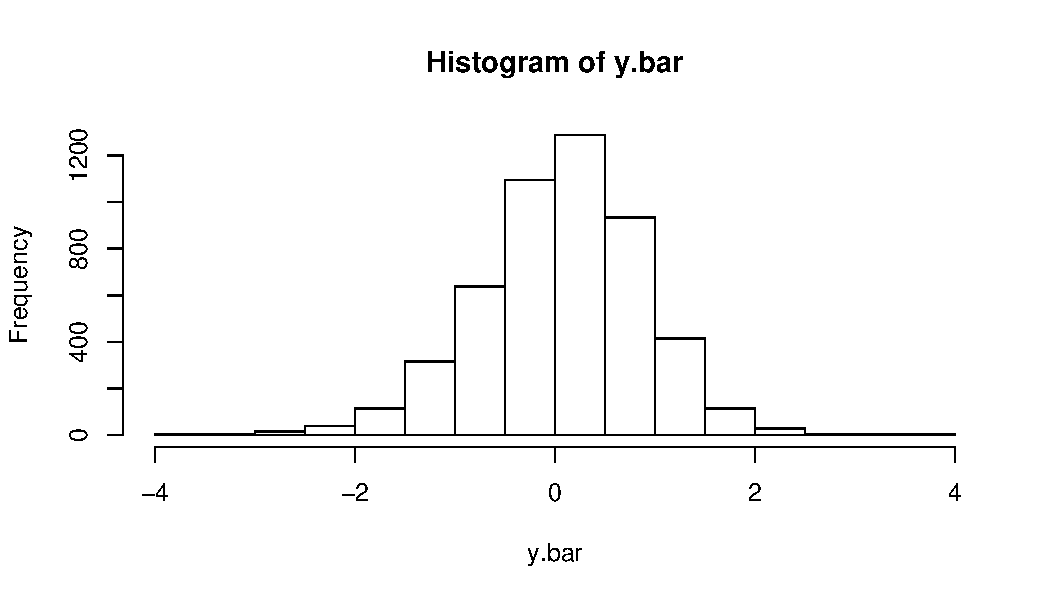
\includegraphics[width=\maxwidth]{figure/unnamed-chunk-36-1} 
\begin{kframe}\begin{alltt}
\hlkwd{mean}\hlstd{(y.bar)}
\end{alltt}
\begin{verbatim}
## [1] 0.068
\end{verbatim}
\begin{alltt}
\hlkwd{sd}\hlstd{(y.bar)}
\end{alltt}
\begin{verbatim}
## [1] 0.81
\end{verbatim}
\begin{alltt}
\hlkwd{quantile}\hlstd{(y.bar,}\hlkwd{c}\hlstd{(}\hlnum{0.025}\hlstd{,}\hlnum{0.975}\hlstd{))}
\end{alltt}
\begin{verbatim}
## 2.5%  98% 
## -1.6  1.6
\end{verbatim}
\end{kframe}
\end{knitrout}
Podemos ver que se espera que el promedio de las pruebas en 5 nuevos pacientes es de 0.068, con un intervalo del 95\% de (-1.6, 1.6), este intervalo es mucho m\'as ancho que el de $\theta$, pues naturalmente $\bar{Y}$ tiene mayor incertidumbre que los par\'ametros del modelo, y en segundo lugar, el tama\~no de nuevos datos es de 5 que es bastante  peque\~no, lo cual hace que el pron\'ostico para $\bar{Y}^*$ no sea muy preciso.
\end{Eje}

\subsection{Par\'ametros dependientes}

En algunas situaciones es muy \'util asumir una distribuci\'on previa conjugada, y para lograr eso no es posible establecer que los par\'ametros tengan distribuciones previa independientes. Bajo esta situaci\'on, la inferencia posterior de los par\'ametros de inter\'es debe ser llevada a cabo en dos etapas: En la primera, se debe establecer la distribuci\'on previa conjunta para ambos par\'ametros siguiendo la sencilla regla que afirma que
\begin{equation*}
p(\theta,\sigma^2)=p(\sigma^2)p(\theta \mid \sigma^2)
\end{equation*}

En la segunda etapa ya es posible analizar propiamente cada uno de los par\'ametros de inter\'es siguiendo otra sencilla regla que afirma que
\begin{equation*}
p(\theta,\sigma^2 \mid \mathbf{Y})\propto p(\mathbf{Y} \mid \theta,\sigma^2)p(\theta,\sigma^2)
\end{equation*}

La anterior formulaci\'on conlleva a asignar una distribuci\'on previa para $\theta$ dependiente del par\'ametro $\sigma^2$. Esto quiere decir que en la distribuci\'on $p(\theta \mid \sigma^2)$, el valor de $\sigma^2$ se considera una constante fija y conocida, esta distribuci\'on previa est\'a dada por\footnote{La forma como la distribuci\'on previa de $\theta$ dependa de $\sigma^2$ es coherente con la informaci\'on de Fisher sobre $\theta$ que es igual a $\sigma^{-2}$.}
\begin{equation*}
p(\theta \mid \sigma^2)\sim Normal(\mu,\sigma^2/c_0)
\end{equation*}

donde $c_0$ es una constante. Por otro lado, y siguiendo los argumentos de la secci\'on 2.7, una posible opci\'on para la distribuci\'on previa de $\sigma^2$, que no depende de $\theta$, corresponde a
\begin{equation*}
p(\sigma^2)\sim Inversa-Gamma(n_0/2,n_0\sigma^2_0/2)
\end{equation*}

De esta forma, podemos encontrar la distribuci\'on conjunta previa de $\theta$ y $\sigma^2$ como sigue:
\begin{Res}
La distribuci\'on conjunta previa de los par\'ametros $\theta$ y $\sigma^2$ est\'a dada por una distribuci\'on
\begin{equation*}
\theta,\sigma^2 \sim Normal-Inversa-Gamma\left(\mu, c_0, \frac{n_0+1}{2},\frac{n_0\sigma^2_0}{2}\right).
\end{equation*}
\end{Res}

\begin{proof}
\begin{align*}
p(\theta,\sigma^2)&=p(\sigma^2)p(\theta \mid \sigma^2)\\
&\propto (\sigma^2)^{-\frac{n_0}{2}-1}\exp\left\{-\dfrac{n_0\sigma_0^2}{2\sigma^2}\right\}
(\sigma^2)^{-\frac{1}{2}}\exp\left\{-\frac{c_0}{2\sigma^2}(\theta-\mu)^2\right\}\\
&= (\sigma^2)^{-\frac{n_0+1}{2}-1}\exp\left\{-\frac{1}{2\sigma^2}\left[n_0\sigma^2_0+c_0(\theta-\mu)^2\right]\right\}
\end{align*}
la cual corresponde a la forma de la funci\'on de densidad de la distribuci\'on Normal-Inversa-Gamma.
\end{proof}

Una vez encontrada la distribuci\'on conjunta previa, procedemos a encontrar la distribuci\'on conjunta posterior, y as\'i poder encontrar las estimaciones de $\theta$ y $\sigma^2$.
\begin{Res}
La distribuci\'on posterior conjunta de los par\'ametros $\theta$ y $\sigma^2$ est\'a dada por
\begin{equation*}
\theta,\sigma^2\mid\mathbf{Y} \sim Normal-Inversa-Gamma\left(\mu_n, c_0+n, \frac{n_0+n+1}{2},\beta\right).
\end{equation*}

con 
\begin{equation*}
\beta=\dfrac{1}{2}\left(n_0\sigma^2_0+(n-1)S^2+\dfrac{c_0n}{c_0+n}(\mu-\bar{y})^2\right)
\end{equation*}

y
\begin{equation*}
\mu_n=\frac{\frac{n}{\sigma^2}\bar{Y}+\frac{c_0}{\sigma^2}\mu}{\frac{n}{\sigma^2}+\frac{c_0}{\sigma^2}}
=\frac{n\bar{Y}+c_0\mu}{n+c_0}
\end{equation*}
\end{Res}

\begin{proof}
En primer lugar, recordamos que la funci\'on de verosimilitud de la muestra est\'a dada por
\begin{align}
p(\mathbf{Y} \mid \theta,\sigma^2)= \frac{1}{(2\pi\sigma^2)^{n/2}}
\exp\left\{-\frac{1}{2\sigma^2}\left[(n-1)S^2+n(\bar{y}-\theta)^2\right]\right\}
\end{align}
Por otro lado, se tiene que
\begin{align}\label{desarro1}
p(\theta,\sigma^2 \mid \mathbf{Y}) & \propto p(\mathbf{Y} \mid \theta,\sigma^2)p(\theta,\sigma^2)\notag\\
&\propto (\sigma^2)^{-\frac{n_0+n+1}{2}-1}
\exp\left\{-\frac{1}{2\sigma^2}\left[n_0\sigma^2_0+c_0(\theta-\mu)^2+(n-1)S^2+n(\bar{y}-\theta)^2\right]\right\}\notag\\
&= (\sigma^2)^{-\frac{n_0+n+1}{2}-1}\\
&\times
\exp\left\{-\frac{1}{2\sigma^2}\left[n_0\sigma^2_0+(n-1)S^2+(c_0+n)(\theta-\mu_n)^2+\frac{c_0n}{c_0+n}(\mu-\bar{y})^2\right]\right\}
\end{align}
puesto que
\begin{align*}
c_0(\theta-\mu)^2+n(\bar{y}-\theta)^2=(c_0+n)(\theta-\mu_n)^2+\frac{c_0n}{c_0+n}(\mu-\bar{y})^2
\end{align*}
\end{proof}

Para encontrar las distribuciones marginales posterior de cada uno de los par\'ametros se procede de la siguiente forma:
  
\begin{enumerate}
\item Para hallar la distribuci\'on posterior condicional de $\theta$, dada por $P(\theta \mid \sigma^2,\mathbf{Y})$, se debe considerar que $\sigma^2$ es una constante fija y conocida tal como se consider\'o al principio de esta secci\'on. Basado en lo anterior, es posible utilizar la siguiente regla de probabilidad
\begin{align*}
P(\theta \mid \sigma^2,\mathbf{Y})=\frac{p(\theta,\sigma^2 \mid \mathbf{Y})}{p(\sigma^2,\mathbf{Y})}p(\mathbf{Y})\propto p(\theta,\sigma^2 \mid \mathbf{Y})
\end{align*}
Lo anterior sugiere que la distribuci\'on marginal posterior de $\theta$, $p(\theta \mid \sigma^2,\mathbf{Y})$, se encuentra utilizando la distribuci\'on posterior conjunta, $p(\theta,\sigma^2 \mid \mathbf{Y})$, suponiendo que todas las expresiones que involucren al valor $\sigma^2$ se pueden incluir en la constante de proporcionalidad
\item Dado que $\sigma^2$ no depende de ning\'un otro par\'ametro entonces, utilizando la distribuci\'on posterior conjunta, es posible encontrar su distribuci\'on marginal posterior de la siguiente forma
\begin{align*}
p(\sigma^2 \mid \mathbf{Y})=\int p(\theta,\sigma^2 \mid \mathbf{Y}) d\theta
\end{align*}

Lo propio es posible hacer con $\theta$, utilizando la distribuci\'on posterior conjunta, es posible encontrar su distribuci\'on marginal posterior de la siguiente forma
\begin{align*}
p(\theta \mid \mathbf{Y})=\int p(\theta,\sigma^2 \mid \mathbf{Y}) d\sigma^2
\end{align*}
\end{enumerate}

\begin{Res}
La distribuci\'on posterior de $\theta$ condicional a $\sigma^2,\mathbf{Y}$ est\'a dada por
\begin{equation*}
\theta \mid \sigma^2,\mathbf{Y} \sim Normal(\mu_n,\sigma^2/(n+c_0))
\end{equation*}
con $\mu_n=\dfrac{n\bar{y}+c_0\mu}{n+c_0}$.
\end{Res}

\begin{proof}
Acudiendo a la distribuci\'on posterior conjunta dada en (\ref{desarro1}), tenemos que
\begin{align*}
p(\theta \mid \sigma^2,\mathbf{Y})&\propto 
p(\theta,\sigma^2 \mid \mathbf{Y}) \\
&\propto(\sigma^2)^{-\frac{n_0+n+1}{2}-1}\\
&\hspace{1cm}\times
\exp\left\{-\frac{1}{2\sigma^2}\left[n_0\sigma^2_0+(n-1)S^2+(c_0+n)(\theta-\mu_n)^2+\frac{c_0n}{c_0+n}(\mu-\bar{y})^2\right]\right\}\\
&\propto \exp\left\{-\frac{1}{2\sigma^2}(c_0+n)(\theta-\mu_n)^2\right\}
\end{align*}
la cual corresponde a la forma de la funci\'on de densidad de la distribuci\'on $Normal(\mu_n, \sigma^2/(n+c_0))$.
\end{proof}

En el anterior resultado, la media de la distribuci\'on condicional posterior $\mu_n$ se puede escribir como $\mu_n=\frac{n}{n+c_0}\bar{y}+\frac{c_0}{n+c_0}\mu$, promedio ponderado entre la estimaci\'on cl\'asica $\bar{y}$ y la estimaci\'on previa $\mu$. Observando la forma que toman los pesos $\frac{n}{n+c_0}$ y $\frac{c_0}{n+c_0}$, se puede pensar a $c_0$ como el n\'umero de observaciones en la informaci\'on previa, y as\'i, los pesos de la estimaci\'on cl\'asica y la estimaci\'on previa dependen directamente de los tama\~nos muestrales respectivos.

\begin{Res}\label{Poster_sigma2_IG}
La distribuci\'on marginal posterior del par\'ametro $\sigma^2$ es
\begin{equation*}
\sigma^2 \mid \mathbf{Y} \sim Inversa-Gamma\left(\frac{n+n_0}{2},\frac{(n+n_0)\sigma^2_n}{2}\right)
\end{equation*}
Donde $(n+n_0)\sigma^2_n=n_0\sigma^2_0+(n-1)S^2+\frac{c_0n}{c_0+n}(\mu-\bar{y})^2$ corresponde a una suma ponderada de la varianza previa, la varianza muestral y la diferencia entre la media muestral y la media previa.
\end{Res}

\begin{proof}
De la distribuci\'on posterior conjunta (\ref{desarro1}) e integrando con respecto a $\theta$, se tiene que
\begin{align*}
p(\sigma^2 \mid \mathbf{Y})&=\int p(\theta,\sigma^2 \mid \mathbf{Y}) \ d\theta\\
&\propto (\sigma^2)^{-\frac{n_0+n+1}{2}-1}
\exp\left\{-\frac{1}{2\sigma^2}\left[n_0\sigma^2_0+(n-1)S^2+\frac{c_0n}{c_0+n}(\mu-\bar{y})^2\right]\right\}\\
&\hspace{2cm}\times
\int_{-\infty}^{\infty}\exp\left\{-\frac{n+c_0}{2\sigma^2}(\theta-\mu_n)^2\right\} \ d\theta\\
&\propto (\sigma^2)^{-\frac{n_0+n}{2}-1}
\exp\left\{-\frac{1}{2\sigma^2}\left[n_0\sigma^2_0+(n-1)S^2+\frac{c_0n}{c_0+n}(\mu-\bar{y})^2\right]\right\}\\
&\hspace{2cm}\times
\int_{-\infty}^{\infty}\frac{\sqrt{n+c_0}}{\sqrt{2\pi\sigma^2}}
\exp\left\{-\frac{n+c_0}{2\sigma^2}(\theta-\mu_n)^2\right\} \ d\theta\\
&\propto (\sigma^2)^{-\frac{n_0+n}{2}-1}
\exp\left\{-\frac{(n+n_0)\sigma^2_n}{2\sigma^2}\right\}
\end{align*}
la cual corresponde a la forma de la funci\'on de densidad de la distribuci\'on $Inversa-Gamma(\frac{n+n_0}{2},\frac{(n+n_0)\sigma^2_n}{2})$.
\end{proof}

Dadas las distribuciones $p(\sigma^2\mid \mathbf{Y})$ y $p(\theta\mid \sigma^2, \mathbf{Y})$, podemos proceder de la siguiente forma para obetener valores simulados de $\theta$ y $\sigma^2$ y as\'i, obtener las estimaciones. Si el n\'umero de iteraciones se fija como $G$, entonces se procede a:

\begin{enumerate}[(1)]
\item Simular $G$ valores de la distribuci\'on de $\sigma^2|\mathbf{Y}$, es decir, de la distribuci\'on $Inversa-Gamma$ encontrada en el anterior resultado, estos valores se denotan por $\sigma^2_{(1)},\sigma^2_{(2)},\cdots,\sigma^2_{(G)}$.
\item  Para cada valor de $\sigma^2_{(g)}$, con $g=1,\cdots,G$, simlar un valor de la distribuci\'on de $\theta|\sigma^2,\mathbf{Y}$, es decir, de la distribuci\'on $N(\mu_n,\sigma^2/(n+c_0))$, donde $\sigma^2$ se reemplaza por $\sigma^2_{(g)}$. De esta forma, se obtiene los valores $\theta_{(1)},\theta_{(2)},\cdots,\theta_{(G)}$.
\end{enumerate}

Es claro que en el anterior algoritmo, no es necesario fijar alg\'un valor inicial para $\theta$ o para $\sigma^2$, as\'i como tampoco induce correlaciones entre los valores simulados para ning\'un par\'ametro. Por lo tanto, se puede usar directamente estos valores para el c\'alculo de las estimaci\'on, y no es necesario descartar los primeros valores simulados, ni realizar el \emph{thinning}.

Ahora bien, existe otra alternativa para obtener la estimaci\'on de $\theta$ y $\sigma^2$: encontrando directamente la distribuci\'on posterior de cada par\'ametro. La distribuci\'on posterior de $\sigma^2$ ya se encontr\'o en el resultado \ref{Poster_sigma2_IG}, resta encontrar la distribuci\'on posterior de $\theta$, la cual se presenta en el siguiente resultado. 

\begin{Res}\label{Pos_theta_t_noestandar}
La distribuci\'on posterior del par\'ametro $\theta$ es la distribuci\'on $t$ no estandarizado con grado de libertad $n_0+n$, el par\'ametro de localizaci\'on $\mu_n=\dfrac{n\bar{Y}+c_0\mu}{n+c_0}$ y el par\'ametro de escala $\dfrac{\sigma_n}{\sqrt{c_0+n}}$ con $(n+n_0)\sigma^2_n=n_0\sigma^2_0+(n-1)S^2+\frac{c_0n}{c_0+n}(\mu-\bar{y})^2$. Esto es, 
\begin{equation*}
\theta \mid \mathbf{Y} \sim t_{n+n_0}\left(\mu_n, \frac{\sigma^2_n}{c_0+n}\right)
\end{equation*}
\end{Res}

\begin{proof}
Partiendo de la distribuci\'on posterior conjunta e integrando con respecto a $\sigma^2$, se tiene que
\begin{align*}
p(\theta \mid \mathbf{Y})&= \int_0^{\infty} p(\theta,\sigma^2 \mid \mathbf{Y}) \ d\sigma^2 \\
&\propto \int_0^{\infty} \left(\frac{1}{\sigma^2}\right)^{\frac{n_0+n+1}{2}+1}
\exp\left\{-\frac{1}{2\sigma^2}\left[(n_0+n)\sigma^2_n+(c_0+n)(\theta-\mu_n)^2\right]\right\} \ d\sigma^2
\end{align*}
Haciendo un cambio de variable tal que
\begin{equation*}
z=\frac{A}{2\sigma^2}, \ \ \ \ \ \ \ \ \ \ \ \text{donde} \ \ \ A=(n_0+n)\sigma^2_n+(c_0+n)(\theta-\mu_n)^2
\end{equation*}
por tanto
\begin{equation*}
d\sigma^2=-\frac{A}{2z^2} \ dz
\end{equation*}
Entonces, volviendo a la integral en cuesti\'on, se tiene que
\begin{align*}
p(\theta \mid \mathbf{Y})& \propto
\left(\frac{1}{A}\right)^{\frac{n_0+n+1}{2}+1}\int_{\infty}^{0} \frac{-A}{2z^2} (2z)^{\frac{n_0+n+1}{2}+1}e^{-z} \ dz \\
&\propto A^{-\frac{n_0+n+1}{2}}\underbrace{\int_{0}^{\infty} z^{\frac{n_0+n+1}{2}-1}e^{-z}\ dz}_{Gamma\left(\frac{n_0+n+1}{2},1\right)}\\
&\propto A^{-\frac{n_0+n+1}{2}}\\
&= \left[(n_0+n)\sigma^2_n+(c_0+n)(\theta-\mu_n)^2\right]^{-\frac{n_0+n+1}{2}}\\
&\propto \left[1+\frac{(c_0+n)(\theta-\mu_n)^2}{(n_0+n)\sigma^2_n}\right]^{-\frac{n_0+n+1}{2}}\\
&=\left[1+\frac{1}{n_0+n}\left(\frac{\theta-\mu_n}{\sigma_n/\sqrt{c_0+n}}\right)^2\right]^{-\frac{n_0+n+1}{2}}
\end{align*}
la cual corresponde a la forma de la funci\'on de densidad de la distribuci\'on deseada.
\end{proof}

Las distribuciones encontradas en los resultados \ref{Poster_sigma2_IG} y \ref{Pos_theta_t_noestandar}, permite estimar directamente los par\'ametros $\theta$ y $\sigma^2$ usando las esperanzas te\'oricas de las distribuciones posteriores. Esto es, las estimaciones puntuales son:
\begin{align*}
\hat{\theta}&=\mu_n=\dfrac{n\bar{Y}+c_0\mu}{n+n_0}\\
\hat{\sigma}^2&=\dfrac{(n+n_0)\sigma^2_n/2}{(n+n_0)/2-1}=\dfrac{(n+n_0)\sigma^2_n}{n+n_0-2}\approx\sigma^2_n=\dfrac{n_0\sigma^2_0+(n-1)S^2+\frac{c_0n}{c_0+n}(\mu-\bar{y})^2}{n+n_0}
\end{align*}

Los intervalos de credibilidad de $\theta$ y $\sigma^2$ de $(1-\alpha)\times 100\%$ se construyen usando los percentiles $\alpha/2$ y $1-\alpha/2$ de las respectivas distribuciones posteriores dadas en los resultados mencionados anteriormente.

Ilustramos el uso de la metodolog\'ia en el siguiente ejemplo.

\begin{Eje}\label{Eje2.1.2}
Para los datos de funci\'on renal \cite{Efronims} que se muestran en el Ejemplo \ref{Eje-Renal}, suponga que la informaci\'on previa est\'a contenida en la medici\'on de funci\'on renal en una muestra de 12 pacientes dadas por: -1.3619, -1.1116, -0.4744, -0.5663, 2.2056, 0.9491, 0.2298, -0.7933, 1.0198, -0.9850, 3.5679 y -1.9504. La media y la varianza muestral de estas 12 observaciones corresponden a 0.060775 y 2.598512, as\'i, se toma $\mu=0.060775$, $\sigma^2_0=2.598512$ y $c_0=n_0=12$. 

Por otro lado, la media y la varianza muestral de los 15 pacientes en la informaci\'on actual son $\bar{y}=0.08349249$ y $S^2=2.301684$. De esta forma, los par\'ametros de las distribuciones marginales posterior de $\theta$ y $\sigma^2$ se pueden calcular como $\mu_n=\frac{15}{15+12}\times 0.08349249+\frac{12}{15+12}\times 0.060775=0.07339583$ y $$\sigma^2_n=\dfrac{12*2.598512+14*2.301684+6.666667*(0.060775-0.08349249)^2}{15+12}=2.348487$$ En conclusi\'on, las distribuciones marginales posterior de $\theta$ y $\sigma^2$ est\'an dadas por
\begin{equation*}
\theta|\mathbf{Y}\sim t_{27}(0.07339583,2.348487/27=0.086981)
\end{equation*}

y
\begin{equation*}
\sigma^2|\mathbf{Y}\sim Inversa-Gamma(27/2=13.5,\ 27*2.348487/2=31.70457)
\end{equation*}

As\'i, la estimaci\'on Bayesiana de $\theta$ es $\mu_n=0.073$ y un intervalo de credibilidad de $95\%$ para $\theta$ se puede calcular como $0.073\pm t_{27,0.975}*\sqrt{0.086981}=(-0.53,\ 0.68)$. Por otro lado, la estimaci\'on Bayesiana de $\sigma^2$ est\'a dada por $31.70457/(13.5-1)=2.53$, y un intervalo de credibilidad de $95\%$ para $\sigma^2$ se puede calcular como los percentiles $2.5\%$ y $97.5\%$ de la distribuci\'on $IG(13.5,\ 31.70457)$, dado por $(1.5, 4.4)$.

Los anteriores c\'alculos se ilustran en el siguiente c\'odigo \verb'R'.
\begin{knitrout}
\definecolor{shadecolor}{rgb}{0.933, 0.933, 0.933}\color{fgcolor}\begin{kframe}
\begin{alltt}
\hlkwd{library}\hlstd{(pscl)}
\hlcom{# Datos de la informacion previa}
\hlstd{x} \hlkwb{<-} \hlkwd{c}\hlstd{(}\hlopt{-}\hlnum{1.3619}\hlstd{,} \hlopt{-}\hlnum{1.1116}\hlstd{,} \hlopt{-}\hlnum{0.4744}\hlstd{,} \hlopt{-}\hlnum{0.5663}\hlstd{,} \hlnum{2.2056}\hlstd{,} \hlnum{0.9491}\hlstd{,} \hlnum{0.2298}\hlstd{,} \hlopt{-}\hlnum{0.7933}\hlstd{,} \hlnum{1.0198}\hlstd{,}
          \hlopt{-}\hlnum{0.9850}\hlstd{,} \hlnum{3.5679}\hlstd{,} \hlopt{-}\hlnum{1.9504}\hlstd{)}
\hlcom{# Datos de la informacion actual}
\hlstd{y} \hlkwb{<-} \hlkwd{c}\hlstd{(}\hlnum{1.69045085}\hlstd{,} \hlopt{-}\hlnum{1.41076082}\hlstd{,} \hlopt{-}\hlnum{0.27909483}\hlstd{,} \hlopt{-}\hlnum{0.91387987}\hlstd{,} \hlnum{3.21868429}\hlstd{,} \hlopt{-}\hlnum{1.47282460}\hlstd{,}
          \hlopt{-}\hlnum{0.96524353}\hlstd{,} \hlopt{-}\hlnum{2.45084934}\hlstd{,} \hlnum{1.03838153}\hlstd{,} \hlnum{1.79928679}\hlstd{,} \hlnum{0.97826621}\hlstd{,} \hlnum{0.67463830}\hlstd{,}
          \hlopt{-}\hlnum{1.08665864}\hlstd{,} \hlopt{-}\hlnum{0.00509027}\hlstd{,} \hlnum{0.43708128}\hlstd{)}
\hlcom{# Paramatros de la distribucion previa}
\hlstd{n0} \hlkwb{<-} \hlstd{c0} \hlkwb{<-} \hlnum{12}
\hlstd{mu} \hlkwb{<-} \hlkwd{mean}\hlstd{(x); sigma2_0} \hlkwb{<-} \hlkwd{var}\hlstd{(x)}
\hlcom{# Informacion}
\hlstd{n} \hlkwb{<-} \hlkwd{length}\hlstd{(y)}
\hlstd{bar.y} \hlkwb{<-} \hlkwd{mean}\hlstd{(y); S2} \hlkwb{<-} \hlkwd{var}\hlstd{(y)}
\hlcom{# Algunos paramatros de la distribucion posterior}
\hlstd{mu.n} \hlkwb{<-} \hlstd{(n}\hlopt{*}\hlstd{bar.y} \hlopt{+} \hlstd{c0}\hlopt{*}\hlstd{mu)}\hlopt{/}\hlstd{(n}\hlopt{+}\hlstd{n0)}
\hlstd{sigma2_n} \hlkwb{<-} \hlstd{(n0}\hlopt{*}\hlstd{sigma2_0}\hlopt{+}\hlstd{(n}\hlopt{-}\hlnum{1}\hlstd{)}\hlopt{*}\hlstd{S2}\hlopt{+}\hlstd{c0}\hlopt{*}\hlstd{n}\hlopt{*}\hlstd{(mu}\hlopt{-}\hlstd{bar.y)}\hlopt{^}\hlnum{2}\hlopt{/}\hlstd{(c0}\hlopt{+}\hlstd{n))}\hlopt{/}\hlstd{(n}\hlopt{+}\hlstd{n0)}
\hlcom{# Estimacion puntual}
\hlstd{theta.hat} \hlkwb{<-} \hlstd{mu.n; sigma2.hat} \hlkwb{<-} \hlstd{(n}\hlopt{+}\hlstd{n0)}\hlopt{*}\hlstd{sigma2_n}\hlopt{/}\hlstd{(n}\hlopt{+}\hlstd{n0}\hlopt{-}\hlnum{2}\hlstd{)}
\hlstd{theta.hat}
\end{alltt}
\begin{verbatim}
## [1] 0.073
\end{verbatim}
\begin{alltt}
\hlstd{sigma2.hat}
\end{alltt}
\begin{verbatim}
## [1] 2.5
\end{verbatim}
\begin{alltt}
\hlcom{# Intervalo de credibilidad de 95% para theta}
\hlstd{mu.n} \hlopt{+} \hlkwd{qt}\hlstd{(}\hlkwd{c}\hlstd{(}\hlnum{0.025}\hlstd{,}\hlnum{0.975}\hlstd{),} \hlkwc{df}\hlstd{=n}\hlopt{+}\hlstd{n0)}\hlopt{*}\hlkwd{sqrt}\hlstd{(sigma2_n}\hlopt{/}\hlstd{(n}\hlopt{+}\hlstd{n0))}
\end{alltt}
\begin{verbatim}
## [1] -0.53  0.68
\end{verbatim}
\begin{alltt}
\hlcom{# Intervalo de credibilidad de 95% para sigma2}
\hlkwd{qigamma}\hlstd{(}\hlnum{0.025}\hlstd{,} \hlkwc{alpha}\hlstd{=(n}\hlopt{+}\hlstd{n0)}\hlopt{/}\hlnum{2}\hlstd{,} \hlkwc{beta}\hlstd{=(n}\hlopt{+}\hlstd{n0)}\hlopt{*}\hlstd{sigma2_n}\hlopt{/}\hlnum{2}\hlstd{)}
\end{alltt}
\begin{verbatim}
## [1] 1.5
\end{verbatim}
\begin{alltt}
\hlkwd{qigamma}\hlstd{(}\hlnum{0.975}\hlstd{,} \hlkwc{alpha}\hlstd{=(n}\hlopt{+}\hlstd{n0)}\hlopt{/}\hlnum{2}\hlstd{,} \hlkwc{beta}\hlstd{=(n}\hlopt{+}\hlstd{n0)}\hlopt{*}\hlstd{sigma2_n}\hlopt{/}\hlnum{2}\hlstd{)}
\end{alltt}
\begin{verbatim}
## [1] 4.4
\end{verbatim}
\end{kframe}
\end{knitrout}

Otra forma de estimar los par\'ametros $\theta$ y $\sigma^2$ es utilizando los m\'etodos de Monte Carlos tal como lo expone anteriormente, simulando primero los valores de $\sigma^2$ y posteriormente los valores de $\theta$.
\begin{knitrout}
\definecolor{shadecolor}{rgb}{0.933, 0.933, 0.933}\color{fgcolor}\begin{kframe}
\begin{alltt}
\hlstd{n.sim} \hlkwb{<-} \hlnum{20000}
\hlstd{sigma2.res} \hlkwb{<-} \hlkwd{rinvgamma}\hlstd{(n.sim, (n}\hlopt{+}\hlstd{n0)}\hlopt{/}\hlnum{2}\hlstd{, (n}\hlopt{+}\hlstd{n0)}\hlopt{*}\hlstd{sigma2_n}\hlopt{/}\hlnum{2}\hlstd{)}
\hlstd{theta.res} \hlkwb{<-} \hlkwd{c}\hlstd{()}
\hlkwa{for}\hlstd{(i} \hlkwa{in} \hlnum{1}\hlopt{:}\hlstd{n.sim)\{}
  \hlstd{theta.res[i]} \hlkwb{<-} \hlkwd{rnorm}\hlstd{(}\hlnum{1}\hlstd{,mu.n,} \hlkwd{sqrt}\hlstd{(sigma2.res[i]}\hlopt{/}\hlstd{(n}\hlopt{+}\hlstd{c0)))}
\hlstd{\}}
\hlcom{# Visualiza los valores simulados}
\hlcom{## par(mfrow=c(1,2))}
\hlcom{## ts.plot(theta.res)}
\hlcom{## ts.plot(sigma2.res)}
\hlcom{## acf(theta.res)}
\hlcom{## acf(sigma2.res)}
\hlcom{# Estimaciones puntuales}
\hlkwd{mean}\hlstd{(theta.res)}
\end{alltt}
\begin{verbatim}
## [1] 0.073
\end{verbatim}
\begin{alltt}
\hlkwd{mean}\hlstd{(sigma2.res)}
\end{alltt}
\begin{verbatim}
## [1] 2.5
\end{verbatim}
\begin{alltt}
\hlcom{# Intervalos de credibilidad del 95%}
\hlkwd{quantile}\hlstd{(theta.res,} \hlkwd{c}\hlstd{(}\hlnum{0.025}\hlstd{,}\hlnum{0.975}\hlstd{))}
\end{alltt}
\begin{verbatim}
##  2.5%   98% 
## -0.53  0.67
\end{verbatim}
\begin{alltt}
\hlkwd{quantile}\hlstd{(sigma2.res,} \hlkwd{c}\hlstd{(}\hlnum{0.025}\hlstd{,}\hlnum{0.975}\hlstd{))}
\end{alltt}
\begin{verbatim}
## 2.5%  98% 
##  1.5  4.4
\end{verbatim}
\end{kframe}
\end{knitrout}

De las gr\'aficas que arrojan los anteriores c\'odigos, se puede comprobar que (1) no hay necesidad de descartar los primeros valores obtenidos, y (2) los valores simulados no incorrelacionados entre ellos, por lo cual podemos calcular las estimaciones directamente usando los 20 mil valores simulados. 

La estimaci\'on e intervalo de credibilidad para $\theta$ calculada desde los valores simulados corresponden a 0.073 y (-0.53, 0.67); mientras que para $\sigma^2$, est\'an dadas por 2.5 y (1.5, 4.4). Podemos ver que los resultados obtenidos en los dos enfoques son muy similares.
\end{Eje}

\subsection{Par\'ametros no informativos}
En esta secci\'on consideramos el tratamiento cuando no tenemos informaci\'on previa disponible. Suponga que $\mathbf{Y}=\{Y_1,\ldots,Y_n\}$ corresponde a una muestra de variables aleatorias con distribuci\'on $Normal(\theta,\sigma^2)$. Luego, la funci\'on de distribuci\'on conjunta o verosimilitud est\'a dada por \ref{vero_normal}
\begin{equation*}
p(\mathbf{Y} \mid \theta, \sigma^2)=\frac{1}{(2\pi\sigma^2)^{n/2}}\exp\left\{-\frac{1}{2\sigma^2}\sum_{i=1}^n(y_i-\theta)^2\right\}
\end{equation*}

En primer lugar suponga que los par\'ametros tienen distribuciones previa independientes y en esta primera etapa se realizar\'a el an\'alisis suponiendo que estas distribuciones son no informativas. Lo anterior implica que la distribuci\'on previa conjunta de los par\'ametros de inter\'es est\'a dada por
\begin{equation}
p(\theta,\sigma^2)=p(\theta)p(\sigma^2)
\end{equation}

Como la distribuci\'on previa de $\theta$ es normal, es f\'acil verificar que \'esta empieza a tener las caracter\'isticas propias de una distribuci\'on no informativa cuando la varianza de la misma se vuelve muy grande, sin importar el valor de la media. Cuando esto sucede, la forma de la distribuci\'on previa de $\theta$ se torna plana y es l\'ogico pensar que puede ser acercada mediante una distribuci\'on constante, tal que
\begin{equation*}
p(\theta)\propto cte
\end{equation*}

Por otro lado, \citeasnoun{Gelman03} afirma que la distribuci\'on Inversa-Gamma, la cual es la distribuci\'on previa para el par\'ametro $\sigma^2$, se vuelve no informativa cuando los hiper-par\'ametros toman valores muy cercanos a cero. De esta forma haciendo tender $\alpha \longrightarrow 0$ y $\beta \longrightarrow 0$, entonces la distribuci\'on previa de $\sigma^2$ se convierte en
\begin{equation*}
p(\sigma^2)\propto \sigma^{-2}
\end{equation*}

la cual coincide con la distribuci\'on previa no informativa de Jeffreys discutida en la secci\'on \ref{Normal_Varianza}. Por lo anterior, la distribuci\'on previa no informativa conjunta estar\'ia dada por
\begin{equation}\label{previa_noinfo_conjunta}
p(\theta,\sigma^2)\propto \sigma^{-2}
\end{equation}

Bajo este marco de referencia se tiene el siguiente resultado sobre la distribuci\'on posterior de $\theta$
\begin{Res}\label{pos_theta_no_informativa}
La distribuci\'on posterior del par\'ametro $\theta$ sigue una distribuci\'on $t$ no estandarizado con grado de libertad $n-1$, el par\'ametro de localizaci\'on $\bar{Y}$ y el par\'ametro de escala $\frac{S^2}{n}$, esto es, 
\begin{equation*}
\theta \mid \mathbf{Y}\sim t_{n-1}\left(\bar{y},\frac{S^2}{n}\right).
\end{equation*}

Donde $(n-1)S^2=\sum_{i=1}^n(Y_i-\bar{Y})^2$. Esta distribuci\'on tambi\'en puede expresarse como
\begin{equation*}
\frac{\theta-\bar{y}}{S/\sqrt{n}} \mid \mathbf{Y} \sim t_{n-1}
\end{equation*}

donde $t_{n-1}$ denota la distribuci\'on $t$ estandarizado con grado de libertad $n-1$.
\end{Res}

\begin{proof}
En primer lugar n\'otese que la distribuci\'on posterior conjunta de los par\'ametros de inter\'es es
\begin{align}\label{prop_theta_sigma2}
p(\theta,\sigma^2 \mid \mathbf{Y})& \propto p(\theta,\sigma^2)p(\mathbf{Y} \mid \theta,\sigma^2) \notag \\
& \propto \frac{1}{\sigma^2}\frac{1}{(2\pi\sigma^2)^{n/2}}\exp\left\{-\frac{1}{2\sigma^2}\sum_{i=1}^n(y_i-\theta)^2\right\} \notag\\
& \propto \left(\frac{1}{\sigma^2}\right)^{n/2+1}
\exp\left\{-\frac{1}{2\sigma^2}\left[\sum_{i=1}^n(y_i-\bar{y})^2+n(\bar{y}-\theta)^2\right]\right\} \notag \\
&= \left(\frac{1}{\sigma^2}\right)^{n/2+1}
\exp\left\{-\frac{1}{2\sigma^2}\left[(n-1)S^2+n(\bar{y}-\theta)^2\right]\right\}
\end{align}
Ahora, para hallar la distribuci\'on marginal posterior de $\theta$ es necesario integrar la anterior expresi\'on con respecto a $\sigma^2$. Con esto, se tiene que
\begin{align*}
p(\theta \mid \mathbf{Y})&= \int_0^{\infty} p(\theta,\sigma^2 \mid \mathbf{Y}) \ d\sigma^2 \\
&\propto \int_0^{\infty} \left(\frac{1}{\sigma^2}\right)^{n/2+1}
\exp\left\{-\frac{1}{2\sigma^2}\left[(n-1)S^2+n(\bar{y}-\theta)^2\right]\right\} \ d\sigma^2
\end{align*}
Haciendo un cambio de variable tal que
\begin{equation*}
z=\frac{A}{2\sigma^2}, \ \ \ \ \ \ \ \ \ \ \ \text{donde} \ \ \ A=(n-1)S^2+n(\bar{y}-\theta)^2
\end{equation*}
por tanto
\begin{equation*}
d\sigma^2=-\frac{A}{2z^2} \ dz
\end{equation*}
Entonces, volviendo a la integral en cuesti\'on, se tiene que
\begin{align*}
p(\theta \mid \mathbf{Y})& \propto
\left(\frac{1}{A}\right)^{n/2+1}\int_{\infty}^{0} \frac{-A}{2z^2} (2z)^{n/2+1}e^{-z} \ dz \\
&\propto A^{-n/2}\underbrace{\int_{0}^{\infty} z^{n/2-1}e^{-z}\ dz}_{Gamma(n/2)}\\
&\propto A^{-n/2}\\
&= [(n-1)S^2+n(\bar{y}-\theta)^2]^{-n/2}\\
&\propto \left[1+\frac{n(\bar{y}-\theta)^2}{(n-1)S^2}\right]^{-n/2}
=\left[1+\frac{1}{n-1}\left(\frac{\bar{y}-\theta}{S/\sqrt{n}}\right)^2\right]^{-\frac{(n-1)+1}{2}}
\end{align*}
la cual corresponde a la funci\'on de densidad de distribuci\'on de una variable aleatoria con distribuci\'on $t_{n-1}(\bar{y},S^2/n)$.
\end{proof}

\begin{Res}\label{pos_sigma2_no_informativa}
La distribuci\'on posterior del par\'ametro $\sigma^2$ sigue una distribuci\'on
\begin{equation*}
\sigma^2 \mid \mathbf{Y} \sim Inversa-Gamma((n-1)/2,(n-1)S^2/2).
\end{equation*}
\end{Res}

\begin{proof}
Utilizando el mismo argumento del anterior resultado, se tiene que
\begin{align*}
p(\sigma^2 \mid \mathbf{Y})&= \int_{-\infty}^{\infty} p(\theta,\sigma^2 \mid \mathbf{Y}) \ d\theta \\
& \propto \int_{-\infty}^{\infty} \left(\frac{1}{\sigma^2}\right)^{n/2+1}
\exp\left\{-\frac{1}{2\sigma^2}\left[(n-1)S^2+n(\bar{y}-\theta)^2\right]\right\} \ d\theta \\
& = \left(\frac{1}{\sigma^2}\right)^{n/2+1} \sqrt{2\pi\sigma^2/n}\exp\left\{-\frac{1}{2\sigma^2}(n-1)S^2\right\}\underbrace{\int_{-\infty}^{\infty} \frac{1}{\sqrt{2\pi\sigma^2/n}} \exp\left\{-\frac{n}{2\sigma^2}(\bar{y}-\theta)^2\right\} \ d\theta}_{\text{vale $1$}} \\
& \propto (\sigma^2)^{-n/2-1/2}\exp\left\{-\frac{1}{2\sigma^2}(n-1)S^2\right\}\\
&= (\sigma^2)^{-\frac{n-1}{2}-1}\exp\left\{-\frac{1}{2\sigma^2}(n-1)S^2\right\}
\end{align*}
la cual corresponde a la funci\'on de densidad de la distribuci\'on $Inversa-Gamma((n-1)/2,(n-1)S^2/2)$.
\end{proof}

De los resultados \ref{pos_theta_no_informativa} y \ref{pos_sigma2_no_informativa}, podemos ver que cuando no se dispone de informaci\'on previa, la estimaci\'on bayesiana de $\theta$ y $\sigma^2$ est\'an dadas por
\begin{align*}
\hat{\theta}_B&=E(\theta\mid\mathbf{Y})=\bar{Y}\\
\hat{\sigma}^2_B&=E(\sigma^2\mid\mathbf{Y})=\dfrac{(n-1)S^2/2}{(n-1)/2-1}=\dfrac{n-1}{n-3}S^2\approx S^2
\end{align*}

Podemos concluir que la estimaci\'on bayesiana de $\theta$ cuando no hay informaci\'on previa es id\'entica a la estimaci\'on cl\'asica de $\theta$, mientas que la de $\sigma^2$ es muy similar a la estimaci\'on cl\'asica.

En cuanto a la estimaci\'on por intervalo de credibilidad, podemos ver que un intervalo de crediblidad de $(1-\alpha)\times 100\%$ est\'a dado por los percentiles $\alpha/2$ y $1-\alpha/2$ de la distribuci\'on $t_{n-1}\left(\bar{Y},\dfrac{S^2}{n}\right)$, se puede ver que estos corresponden a $\bar{Y}+t_{n-1,\alpha/2}\dfrac{S}{\sqrt{n}}$ y $\bar{Y}+t_{n-1,1-\alpha/2}\dfrac{S}{\sqrt{n}}$. En conclusi\'on, un intervalo de credibildad para $\theta$ est\'a dado por $\bar{Y}\pm t_{n-1,1-\alpha/2}\dfrac{S}{\sqrt{n}}$, el cual es id\'entico al intervalo de confianza para $\theta$ en la estad\'istica cl\'asica.

En cuanto al intervalo de crediblidad para $\sigma^2$, este est\'a dado por los percentiles $\alpha/2$ y $1-\alpha/2$ de la distribuci\'on $Inversa-Gamma((n-1)/2,\ (n-1)S^2/2)$. En la estad\'istica cl\'asica, el intervalo de confianza para $\sigma^2$ est\'a dada por \begin{equation*}
IC(\sigma^2)=\left(\dfrac{(n-1)S^2}{\chi^2_{n-1,1-\alpha/2}},\ \dfrac{(n-1)S^2}{\chi^2_{n-1,\alpha/2}}\right)
\end{equation*}

Aunque la forma de estos dos intervalos son muy diferentes, resultan ser id\'enticos. A continuaci\'on mostramos el porqu\'e. Suponga que $a$ es el percentil $\alpha/2$ de la distribuci\'on $Inversa-Gamma((n-1)/2,\ (n-1)S^2/2)$, esto es, si $X\sim Inversa-Gamma((n-1)/2,\ (n-1)S^2/2)$, entonces $Pr(X<a)=\alpha/2$. Ahora por propiedades de la distribuci\'on $Inversa-Gamma$, se tiene que $\dfrac{X}{(n-1)S^2}\sim Inversa-Gamma(\frac{n-1}{2},\ \frac{1}{2})$. Por la relaci\'on entre la distribuci\'on $Gamma$ y la distribuci\'on $Inversa-Gamma$, tenemos que $\dfrac{(n-1)S^2}{X}\sim Gamma(\frac{n-1}{2},\ 2)$, es decir, $\dfrac{(n-1)S^2}{X}\sim\chi^2_{n-1}$, de donde tenemos que
\begin{align*}
\frac{\alpha}{2}&=Pr(X<a)\\
&=Pr\left(\dfrac{(n-1)S^2}{X}>\dfrac{(n-1)S^2}{a}\right)
\end{align*}

Esto es, $\dfrac{(n-1)S^2}{a}$ es el percentil $1-\alpha/2$ de la distribuci\'on $\chi^2_{n-1}$, esto es,  $\dfrac{(n-1)S^2}{a}=\chi^2_{n-1,1-\alpha/2}$, de donde $a=\dfrac{(n-1)S^2}{\chi^2_{n-1,1-\alpha/2}}$, as\'i concluimos que el l\'imite inferior del intervalo de credibildad coincide con el l\'imite inferior del intervalo de confianza. An\'alogamente se puede ver que tambi\'en los l\'imites superiores coinciden, y as\'i vemos que el intervalo para $\sigma^2$ coincide en la estad\'istica cl\'asica y la estad\'istica bayesiana sin informaci\'on previa.

\textbf{\emph{Enfoque alterno para estimar $\theta$ y $\sigma^2$}}

Existe otra forma de obtener las estimaciones para el par\'ametro $\theta$, recordando la expresi\'on \ref{prop_theta_sigma2}, podemos afirmar que 
\begin{equation*}
\theta \mid \sigma^2, \mathbf{Y} \sim Normal(\bar{y},\sigma^2/n)
\end{equation*}

puesto que 
\begin{align*}
p(\theta \mid \sigma^2,\mathbf{Y})&\propto p(\theta, \sigma^2 \mid\mathbf{Y})\\
&\propto\exp\left\{-\frac{1}{2\sigma^2}\left[(n-1)S^2+n(\bar{y}-\theta)^2\right]\right\}\\
&=\exp\left\{-\frac{n}{2\sigma^2}(\bar{y}-\theta)^2\right\}
\end{align*}

la cual corresponde a la funci\'on de densidad de la distribuci\'on $Normal(\bar{y},\sigma^2/n)$. De esta forma, usando las distribuci\'on $p(\sigma^2\mid\mathbf{Y})$ y $p(\theta\mid\sigma^2,\mathbf{Y})$, podemos implementar el siguiente procedimiento para obtener valores simulados de $\theta$ y $\sigma^2$: 

Si el n\'umero de iteraciones se fija como $G$, entonces se procede a:
\begin{enumerate}[(1)]
\item Simular $G$ valores de la distribuci\'on de $\sigma^2|\mathbf{Y}$, es decir, de la distribuci\'on $Inversa-Gamma((n-1)/2,(n-1)S^2/2)$, estos valores se denotan por $\sigma^2_{(1)},\sigma^2_{(2)},\cdots,\sigma^2_{(G)}$.
\item  Para cada valor de $\sigma^2_{(g)}$, con $g=1,\cdots,G$, simlar un valor de la distribuci\'on de $\theta|\sigma^2,\mathbf{Y}$, es decir, de la distribuci\'on $N(\bar{y},\sigma^2/n)$, donde $\sigma^2$ se reemplaza por $\sigma^2_{(g)}$. De sta forma, se obtiene los valores $\theta_{(1)},\theta_{(2)},\cdots,\theta_{(G)}$.
\end{enumerate}

Las estimaciones de $\theta$ y $\sigma^2$ se pueden obteer de los valores obtenidos $\theta_{(1)},\theta_{(2)},\cdots,\theta_{(G)}$ y $\sigma^2_{(1)},\sigma^2_{(2)},\cdots,\sigma^2_{(G)}$.

\textbf{\emph{Distribuci\'on predictiva}}

La distribuci\'on predictiva para una nueva observaci\'on $\tilde{Y}$ est\'a dada por 
\begin{align*}
p(\tilde{y}\mid\mathbf{Y})
&=\int\int p(\tilde{y}\mid\theta,\sigma^2) p(\theta,\sigma^2\mid\mathbf{Y})\ d\theta\ d\sigma^2\\
&=\int\int p(\tilde{y}\mid \theta,\sigma^2)p(\theta\mid\sigma^2,\mathbf{Y})p(\sigma^2\mid\mathbf{Y})\ d\theta\ d\sigma^2\\
&=\int\left(\int p(\tilde{y}\mid \theta,\sigma^2)p(\theta\mid\sigma^2,\mathbf{Y})\ d\theta\right)p(\sigma^2\mid\mathbf{Y})\ d\sigma^2\\
\end{align*}

En la integral dentro del par\'entesis, el par\'ametro $\sigma^2$ permanece fijo, por lo cual, dicha integral es la misma a la del resultado \ref{pred_y_theta}, y corresponde a la distribuci\'on $N\left(\bar{y},\left(1+\dfrac{1}{n}\right)\sigma^2\right)$. De esta forma, combinando con la distribuci\'on posterior de $\sigma^2$, tenemos que
\begin{align*}
&\ \ \ \ p(\tilde{y}\mid\mathbf{Y})\\
&=\int_0^\infty \dfrac{1}{\sqrt{2\pi(1+\frac{1}{n})\sigma^2}}\exp\left\{-\dfrac{1}{2\sigma^2(1+\frac{1}{n})}(\tilde{y}-\bar{y})^2\right\}\dfrac{\left(\frac{(n-1)S^2}{2}\right)^{(n-1)/2}}{\Gamma\left(\frac{n-1}{2}\right)}(\sigma^2)^{-\frac{n-1}{2}-1}\exp\left\{-\dfrac{(n-1)S^2}{2\sigma^2}\right\}\ d\sigma^2
\end{align*}

Despu\'es de realizar las manipulaciones algebr\'aicas necesarias, se encuentra que 
\begin{equation}\label{post_y_no_informativa_t_student}
p(\tilde{y}\mid\mathbf{Y})=\dfrac{\Gamma(n/2)}{\Gamma((n-1)/2)}\dfrac{1}{\sqrt{\pi(n-1)}}\left(\left(1+\frac{1}{n}\right)S^2\right)^{-1/2}\left(1+\dfrac{1}{n-1}\dfrac{(\tilde{y}-\bar{y})^2}{\left(1+\frac{1}{n}\right)S^2}\right)^{-n/2}
\end{equation}

la cual corresponde a la distribuci\'on $t$ no estandarizado con grado de libertad $n-1$, el par\'ametro de localizaci\'on $\bar{y}$ y el par\'ametro de escala $(1+\frac{1}{n})S^2$. De esta forma, podemos ver que los dos primeros momentos de esta distribuci\'on est\'an dados por
\begin{align*}
E(\tilde{Y}\mid\mathbf{Y})&=\bar{y}\\
Var(\tilde{Y}\mid\mathbf{Y})&=\dfrac{n-1}{n-3}\left(1+\frac{1}{n}\right)S^2=\dfrac{(n-1)(n+1)}{n(n-3)}S^2
\end{align*}

Otra manera equivalente de conocer el comportamiento probabil\'istico de $\tilde{y}$ es por medio de la simulaci\'on. Se debe simular en primer lugar valores de $\theta$ y de $\sigma^2$ de la distribuci\'on posterior $p(\theta,\ \sigma^2\mid\mathbf{Y})$ usando el muestreador de Gibbs y posteriormente se simula valores de $\tilde{y}$ de la distribuci\'on $p(\tilde{y}\mid\theta,\ \sigma^2)$. En la figura \ref{predictiva_y_priori_noninformative} se muestran el histograma de 10 mil valores de $\tilde{Y}$ simulados de esta forma, donde los datos muestrales corresponden a 20 datos simulados de la distribuci\'on $N(12,3^2)$. En la misma gr\'afica se observa tambi\'en la funci\'on de densidad de la distribuci\'on $t$, podemos ver que los valores de simulados de $\tilde{Y}$ efectivamente coincide con la distribuci\'on predictiva de $\tilde{Y}$. Por lo anterior, se puede calcular un predictor de $\tilde{Y}$ como el promedio de los 10 mil valores simulados, y calcular el intervalo de predicci\'on usando los percentiles de estos 10 mil valores.
 
\begin{figure}[!htb]\label{predictiva_y_priori_noninformative}
\centering
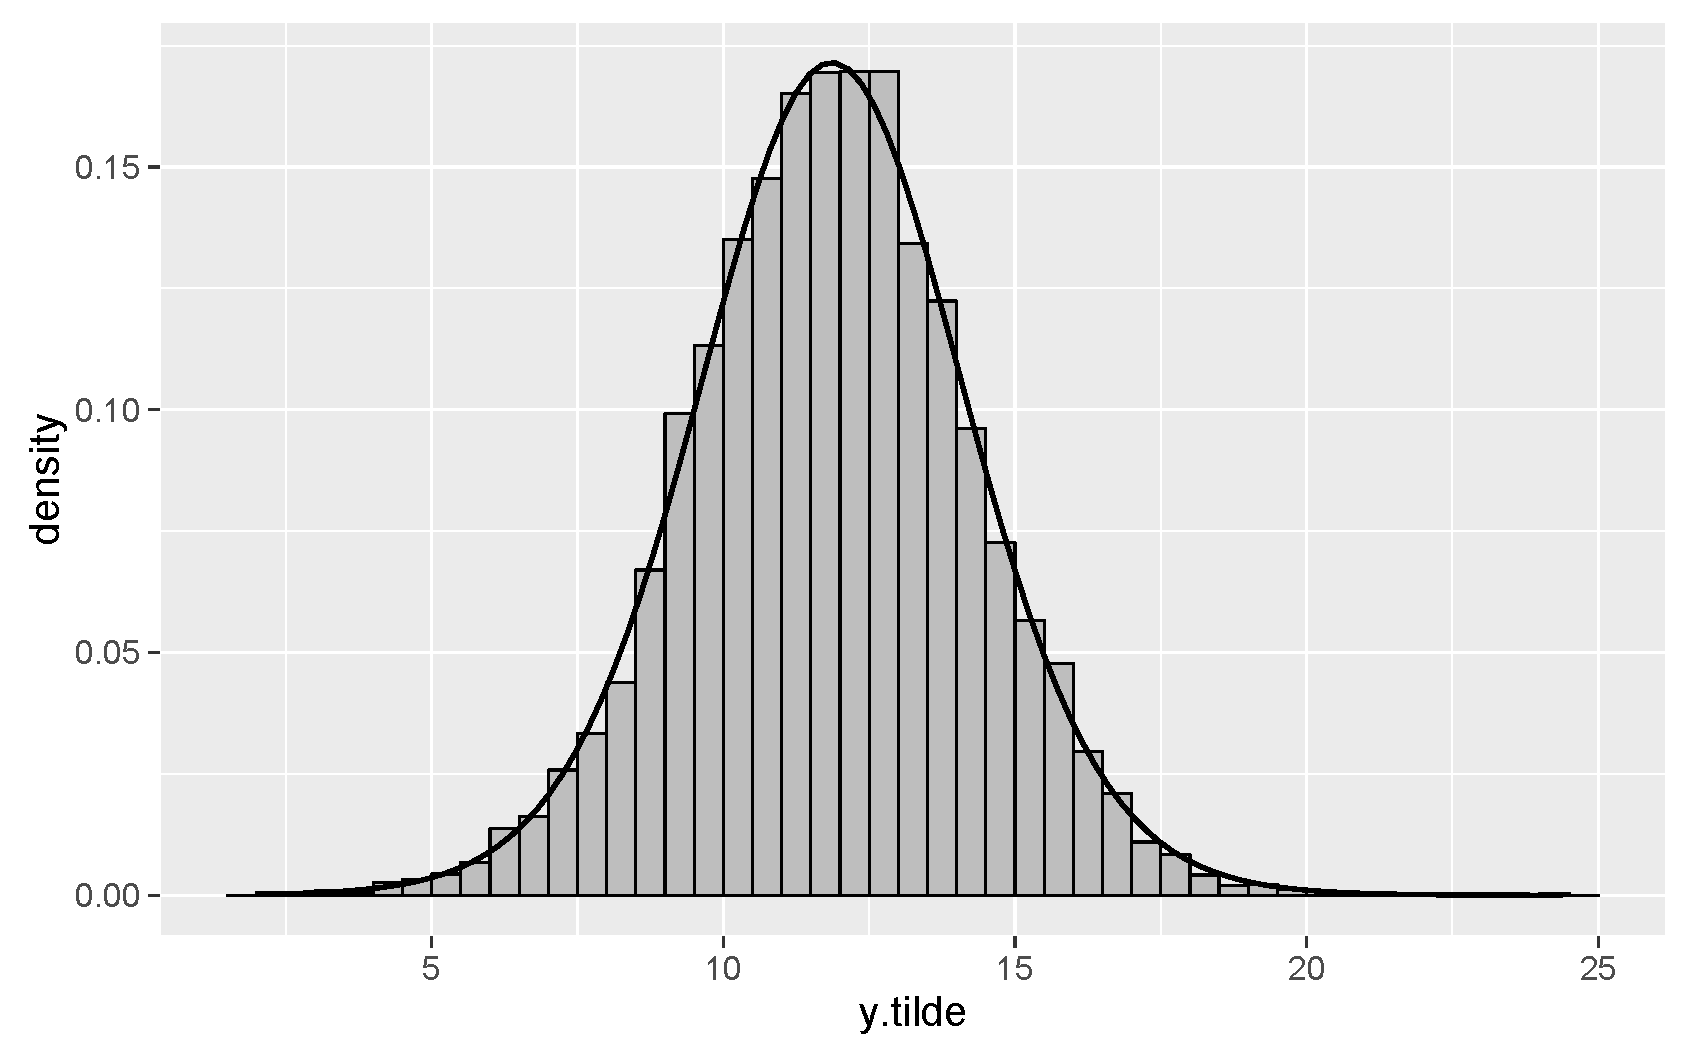
\includegraphics[scale=0.5]{predictiva_y_priori_noninformative.pdf}
\caption{\emph{10 mil valores simulados de $\tilde{Y}$ y la funci\'on de densidad de la distribuci\'on predictiva de $\tilde{Y}$.}}
\end{figure}

\section{Normal multivariante con media desconocida y varianza conocida}

Cuando la distribuci\'on usada para describir el comportamiento de los datos es una distribuci\'on normal multivariante, las t\'ecnicas de inferencia no se distancian mucho del caso univariado. Se debe tener en cuenta el manejo matricial de las formas cuadr\'aticas y las propiedades b\'asicas del c\'alculo de matrices. Los desarrollos y resultados derivados de esta secci\'on redundar\'an en el an\'alisis de los modelos lineales con el enfoque bayesiano.

Sea $\mathbf{Y}=(Y_1,\ldots,Y_p)'$ un vector aleatorio cuya distribuci\'on es normal multivariante dada por

\begin{equation}
p(\mathbf{Y} \mid \btheta,\bSigma)\propto \mid \bSigma \mid ^{-1/2}
\exp\left\{-\frac{1}{2}(\mathbf{y}-\btheta)'\bSigma^{-1}(\mathbf{y}-\btheta)\right\}
  \end{equation}
  
en donde $\btheta=(\theta_1,\ldots,\theta_p)'$ es el vector que contiene la media de cada uno de los componentes del vector $\mathbf{Y}$ y $\bSigma$ es la matriz de varianzas y covarianzas de orden $p\times p$, sim\'etrica y definida positiva. La verosimilitud para una muestra de $n$ vectores aleatorios  independientes e id\'enticamente distribuidos est\'a dada por

\begin{equation*}\label{Vero_Multi}
  p(\mathbf{Y}_1\ldots,\mathbf{Y}_n \mid \btheta,\bSigma)\propto \mid \bSigma \mid ^{-n/2}
  \exp\left\{-\frac{1}{2}\sum_{i=1}^n(\mathbf{y}_i-\btheta)'\bSigma^{-1}(\mathbf{y}_i-\btheta)\right\}
\end{equation*}
    
Los par\'ametros que requieren estimaci\'on corresponden al vector de medias $\btheta$ y la matriz de varianzas y covarianzas $\bSigma$. Por ahora, se asume que $\bSigma$ es conocida y nos centramos en la estimaci\'on del vector de medias $\btheta$. Para la distribuci\'on previa, considerando que en general no hay restricci\'on sobre los valores de los componentes de $\btheta$, asumimos que $\btheta$ sigue una distribuci\'on previa normal multivariante informativa y parametrizada por los hiper par\'ametros $\bmu$ y $\bGamma$
  \begin{equation*}
p(\btheta \mid \bmu,\bGamma)\propto \mid \bGamma \mid ^{-1/2}
\exp\left\{-\frac{1}{2}(\btheta-\bmu)'\bGamma^{-1}(\btheta-\bmu)\right\}
  \end{equation*}
    
%N\'otese que esta distribuci\'on se hace no informativa cuando $ \mid \bGamma^{-1} \mid \longrightarrow 0$ sin importar el valor del vector de medias previa $\bmu$.
En el siguiente resultado, encontramos la distribuci\'on posterior del par\'ametro $\btheta$.
\begin{Res}\label{res_mu_n}
La distribuci\'on posterior del vector $\btheta$ sigue una distribuci\'on normal multivariante
\begin{equation*}
\btheta \mid \mathbf{Y},\bSigma \sim N_p (\bmu_n,\bGamma_n).
\end{equation*}

En donde
\begin{align}
\bGamma_n &= \left(\bGamma^{-1}+n\bSigma^{-1}\right)^{-1}\label{Gamma_n}\\
\bmu_n &= \bGamma_n(\bGamma^{-1}\bmu+n \bSigma^{-1}\bar{\mathbf{y}})\label{mu_n}
\end{align}
\end{Res}

\begin{proof}
En primer lugar, n\'otese la siguiente identidad
\begin{equation}
\sum_{i=1}^n(\mathbf{Y}_i-\btheta)'\bSigma^{-1}(\mathbf{Y}_i-\btheta)
=\sum_{i=1}^n(\mathbf{Y}_i-\bar{\mathbf{Y}})'\bSigma^{-1}(\mathbf{Y}_i-\bar{\mathbf{Y}})
+n(\bar{\mathbf{Y}}-\btheta)'\bSigma^{-1}(\bar{\mathbf{Y}}-\btheta)
\end{equation}

puesto que
\begin{align*}
&\ \ \ \ \sum_{i=1}^n(\mathbf{Y}_i-\btheta)'\bSigma^{-1}(\mathbf{Y}_i-\btheta)\\
&=\sum_{i=1}^n(\mathbf{Y}_i-\bar{\mathbf{Y}}+\bar{\mathbf{Y}}-\btheta)'
\bSigma^{-1}(\mathbf{Y}_i-\bar{\mathbf{Y}}+\bar{\mathbf{Y}}-\btheta)\\
&=\sum_{i=1}^n(\mathbf{Y}_i-\bar{\mathbf{Y}})'\bSigma^{-1}(\mathbf{Y}_i-\bar{\mathbf{Y}})
+\sum_{i=1}^n(\mathbf{Y}_i-\bar{\mathbf{Y}})'\bSigma^{-1}(\bar{\mathbf{Y}}-\btheta)\\
&\hspace{1.5cm}
+(\bar{\mathbf{Y}}-\btheta)'\bSigma^{-1}\sum_{i=1}^n(\mathbf{Y}_i-\bar{\mathbf{Y}})'
+\sum_{i=1}^n(\bar{\mathbf{Y}}-\btheta)'\bSigma^{-1}(\bar{\mathbf{Y}}-\btheta)\\
&=\sum_{i=1}^n(\mathbf{Y}_i-\bar{\mathbf{Y}})'\bSigma^{-1}(\mathbf{Y}_i-\bar{\mathbf{Y}})
+n(\bar{\mathbf{Y}}-\btheta)'\bSigma^{-1}(\bar{\mathbf{Y}}-\btheta)
\end{align*}

Por otro lado, de la definici\'on de distribuci\'on previa, se tiene que
\begin{align*}
p(\btheta \mid \mathbf{Y},\bSigma)
&\propto p(\mathbf{Y} \mid \btheta,\bSigma)p(\btheta,\bSigma)\\
&\propto \exp\left\{-\frac{1}{2}\left[\sum_{i=1}^n(\mathbf{y}_i-\btheta)'\bSigma^{-1}(\mathbf{y}_i-\btheta)+(\btheta-\bmu)'\bGamma^{-1}(\btheta-\bmu)\right]\right\}\\
&\propto \exp\left\{-\frac{1}{2}\left[n(\bar{\mathbf{y}}-\btheta)'\bSigma^{-1}(\bar{\mathbf{y}}-\btheta)+(\btheta-\bmu)'\bGamma^{-1}(\btheta-\bmu)\right]\right\}\\
&\propto \exp\left\{-\frac{1}{2}\left[
  -n\bar{\mathbf{y}}'\bSigma^{-1}\btheta-n\btheta'\bSigma^{-1}\bar{\mathbf{y}}+n\btheta'\bSigma^{-1}\btheta+\btheta'\bGamma^{-1}\btheta-\btheta'\bGamma^{-1}\bmu-\bmu'\bGamma^{-1}\btheta\right]\right\}\\
&= \exp\left\{-\frac{1}{2}\left[
  \btheta'(\bGamma^{-1}+n\bSigma^{-1})\btheta-2\btheta'(\bGamma^{-1}\bmu+n\bSigma^{-1}\bar{\mathbf{y}})\right]\right\}\\
&= \exp\left\{-\frac{1}{2}\left[\btheta'\bGamma^{-1}_n\btheta-2\btheta'\bGamma^{-1}_n\bmu_n\right]\right\}\\
&\propto \exp\left\{-\frac{1}{2}\left[\btheta'\bGamma^{-1}_n\btheta-2\btheta'\bGamma^{-1}_n\bmu_n+\bmu_n\bGamma_n^{-1}\bmu_n\right]\right\}\\
&= \exp\left\{-\frac{1}{2}(\btheta-\bmu_n)'\bGamma_n^{-1}(\btheta-\bmu_n)\right\}
  \end{align*}

La cual corresponde al n\'ucleo de una distribuci\'on normal multivariante con el vector de medias $\bmu_n$ y matriz de varianzas $\bGamma_n$.
\end{proof}

Observando los par\'ametros de la distribuci\'on posterior, podemos ver que $\bGamma_n^{-1} = \bGamma^{-1}+(\bSigma/n)^{-1}$. Teniendo en cuenta que la matriz de varianzas y covarianzas es una medida de dispersi\'on de la distribuci\'on alrededor de su media, la inversa de dicha matriz se puede ver como una medida de precisi\'on de qu\'e tanto se concentra la distribuci\'on alrededor de la media. As\'i, podemos ver que la precisi\'on posterior viene siendo la suma entre la precisi\'on previa y la precisi\'on de la estaimaci\'on cl\'asica del par\'ametro $\btheta$.

En cuanto a la media posterior $\bmu_n$, tenemos que
\begin{align*}
\bmu_n&=\left(\bGamma^{-1}+n\bSigma^{-1}\right)^{-1}
(\bGamma^{-1}\bmu+n \bSigma^{-1}\bar{\mathbf{y}})\\
&=\left(\mathbf{I}+n\bGamma\bSigma^{-1}\right)^{-1}\bmu+\left(\frac{1}{n}\bSigma\bGamma^{-1}+\mathbf{I}\right)^{-1}\bar{\mathbf{y}}\\
&=\underbrace{\bSigma\left(\bSigma+n\bGamma\right)^{-1}}_{\mathbf{A}_1}\bmu+\underbrace{n\bGamma\left(\bSigma+n\bGamma\right)^{-1}}_{\mathbf{A}_2}\bar{\mathbf{y}}
\end{align*}

De donde podemos que ver que la media posterior $\bmu_n$ se puede escribir como $\bmu_n=\mathbf{A}_1\bmu+\mathbf{A}_2\bar{\mathbf{y}}$ donde $\mathbf{A}_1+\mathbf{A}_2=\mathbf{I}$. Es claro que en el caso univariado, $\mathbf{A}_1$, $\bmu$, $\mathbf{A}_2$ y $\bar{\mathbf{y}}$ son todos escalares, y $\bmu_n$ es un valor intermedio entre $\bmu$ y $\bar{\mathbf{y}}$. Mientras que en caso multivariado, $\mathbf{A}_1\bmu+\mathbf{A}_2\bar{\mathbf{y}}$ es similar a una combinaci\'on convexa entre los vectores $\bmu$ y $\bar{\mathbf{y}}$, pero los coeficientes son matrices en vez de escalares. 

Para ilustar la relaci\'on de $\bmu_n$ con $\bmu$ y $\bar{\mathbf{y}}$, tomamos el caso de $p=2$, y denotamos $\mathbf{A}=\bSigma\left(\bSigma+n\bGamma\right)^{-1}$. Es claro que $\mathbf{A}$ es una matriz sim\'etrica y definida positiva, lo denotaremos con $\mathbf{A}_1=\begin{pmatrix}a_{11}&a_{12}\\ a_{12}&a_{22}\end{pmatrix}$, donde $a_{11}>0$ y $a_{22}>0$. De esta forma
\begin{align*}
\bmu_n&=\begin{pmatrix}a_{11}&a_{12}\\ a_{12}&a_{22}\end{pmatrix}\begin{pmatrix}\mu_{1}\\ \mu_{2}\end{pmatrix}+\begin{pmatrix}1-a_{11}&-a_{12}\\ -a_{12}&1-a_{22}\end{pmatrix}\begin{pmatrix}\bar{y}_{1}\\ \bar{y}_{2}\end{pmatrix}\\
&=\begin{pmatrix}a_{11}\mu_1+(1-a_{11})\bar{y}_{1}+a_{12}(\mu_2-\bar{y}_{2})\\a_{22}\mu_2+(1-a_{22})\bar{y}_{2}+a_{12}(\mu_1-\bar{y}_{1})\end{pmatrix}
\end{align*}

Al observar la primera entrada de $\bmu_n$, podemos ver que este se compone de una combinaci\'on convexa entre $\mu_1$ y $\bar{y}_1$ (pues $a_{11}>0$) y una parte que depende de la diferencia $\mu_2-\bar{y}_{2}$; un comportamiento silimar se observa en la segunda entrada de $\bmu_n$. Esta observaci\'on es interesante, pues ilustra que cada componente de la media posterior $\bmu_n$ no siempre ser\'a un promedio ponderado del componentes corrspondiente de la media previa y la estimaci\'on cl\'asica.

Ilustramos los resultados encontrados suponiendo las dos siguientes situaciones 
\begin{enumerate} 
\item Supong que se quiere estimar el vector de medias $\btheta=(\theta_1,\theta_2)'$ con una matriz de varianzas y covarianzas conocida de $\bSigma=\begin{pmatrix}20&8\\ 8&30\end{pmatrix}$. Para eso tenemos 10 datos que corresponden a vectores bivariadas con $\bar{\mathbf{y}}=(150,230)'$. Como informaci\'on previa, suponga que $\bmu=(100,200)'$ y $\bGamma=\begin{pmatrix}5&3\\ 3&10\end{pmatrix}$. C\'alculos arrojan que $\bGamma_n=\begin{pmatrix}1.42&0.64\\ 0.64&2.31\end{pmatrix}$, $\mathbf{A}=\begin{pmatrix}0.3&-0.026\\ -0.026&0.235\end{pmatrix}$ y $\bmu_n=(136,224)$, podemos ver que en este caso, cada componente de $\bmu_n$ se encuentra entre los componentes correspondientes de $\bmu$ y $\bar{\mathbf{y}}$. Los c\'odigos computacionales se muestran a continuaci\'on.
\begin{knitrout}
\definecolor{shadecolor}{rgb}{0.933, 0.933, 0.933}\color{fgcolor}\begin{kframe}
\begin{alltt}
\hlstd{n} \hlkwb{<-} \hlnum{10}
\hlstd{mu} \hlkwb{<-} \hlkwd{matrix}\hlstd{(}\hlkwd{c}\hlstd{(}\hlnum{100}\hlstd{,}\hlnum{200}\hlstd{)); y.bar} \hlkwb{<-} \hlkwd{matrix}\hlstd{(}\hlkwd{c}\hlstd{(}\hlnum{150}\hlstd{,}\hlnum{230}\hlstd{))}
\hlstd{Gamma} \hlkwb{<-} \hlkwd{matrix}\hlstd{(}\hlkwd{c}\hlstd{(}\hlnum{5}\hlstd{,}\hlnum{3}\hlstd{,}\hlnum{3}\hlstd{,}\hlnum{10}\hlstd{),}\hlnum{2}\hlstd{,}\hlnum{2}\hlstd{); Sigma} \hlkwb{<-} \hlkwd{matrix}\hlstd{(}\hlkwd{c}\hlstd{(}\hlnum{20}\hlstd{,}\hlnum{8}\hlstd{,}\hlnum{8}\hlstd{,}\hlnum{30}\hlstd{),}\hlnum{2}\hlstd{,}\hlnum{2}\hlstd{)}
\hlstd{Gamma.n} \hlkwb{<-} \hlkwd{solve}\hlstd{(}\hlkwd{solve}\hlstd{(Gamma)} \hlopt{+} \hlstd{n}\hlopt{*}\hlkwd{solve}\hlstd{(Sigma))}
\hlstd{A} \hlkwb{<-} \hlstd{Sigma} \hlopt \hlkwd{solve}\hlstd{(Sigma} \hlopt{+} \hlstd{n}\hlopt{*}\hlstd{Gamma)}
\hlstd{mu.n} \hlkwb{<-} \hlstd{Gamma.n} \hlopt \hlstd{(}\hlkwd{solve}\hlstd{(Gamma)}\hlopt\hlstd{mu} \hlopt{+} \hlstd{n}\hlopt{*}\hlkwd{solve}\hlstd{(Sigma)}\hlopt\hlstd{y.bar)}
\end{alltt}
\end{kframe}
\end{knitrout}
\item Tomamos los mismo datos del caso anterior, pero suponga que $\bar{\mathbf{y}}=(150,2300)'$, las matrices $\bGamma_n$ y $\mathbf{A}$ no cambian de valor, pero la media de la distribuci\'on posterior est\'a dada por $\bmu_n=(190,1808)$. Podemos ver que el primer componente de $\bmu_n$ no est\'a entre 100 y 150 que corresponden a las estimaciones previa y cl\'asica, respectivamente, esto se debe a que la diferencia entre $\mu_2$ y $\bar{y}_2$ es muy grande.
\end{enumerate}

\textbf{Distribuci\'on previa no informativa}

Al tener en cuenta que la distribuci\'on previa del par\'ametro $\btheta$ es la distribuci\'on normal multivariada, y al observar la forma de la funci\'on de densidad, se puede afirmar que cuando $|\bGamma^{-1}|$ es muy peque\~no, los par\'ametros previas $\bmu$ y $\bGamma$ pierden peso en los c\'alculos de $\bmu_n$ y $\bGamma_n$. En este caso se puede ver que
\begin{align*}
\bGamma_n&\approx n^{-1}\bSigma\\
\bmu_n&\approx \bar{\mathbf{y}}
\end{align*}

De donde podemos concluir que la estimaci\'on bayesiana ser\'a muy cercana a la estimaci\'on cl\'asica $\bar{y}$, m\'as a\'un, el intervalo de credibilidad tambi\'en ser\'a muys similar al intervalo de confianza del enfoque cl\'asico.

\begin{Eje}\label{Eje_Student}
\citeasnoun{Student} introdujo un conjunto de datos cl\'asicos sobre el incremento en horas de sue\~no producido con 2 medicamentos sopor\'iferos diferentes comparados con grupo control en 10 pacientes. Estos datos se pueden encontrar en \verb'R' con nombre \verb'sleep'. Estos datos se pueden ver como realizaciones de vectores aleatorios con distribuci\'on normal bivariada. Supongamos que la matriz de varianzas y covarianzas de la distribuci\'on es conocida e igual a $\Sigma=\begin{pmatrix}1&0.6\\ 0.6&2\end{pmatrix}$, y el par\'ametro de inter\'es es el vector de medias $\btheta=(\theta_1,\theta_2)'$. Para la distribuci\'on previa, suponemos que $\bmu=(0,1)'$, es decir que el primer medicamento no tiene ning\'un efecto sopor\'ifero, mientras que el segundo medicamento tiene un efecto promedio de aumentar 1 hora de sue\~no, tambi\'en asumimos que $\Gamma=\begin{pmatrix}2&0\\ 0&2\end{pmatrix}$. Los siguientes c\'odigos de \verb'JAGS' ilustra el procedimiento de estimaci\'on del par\'ametro de inter\'es.

\begin{knitrout}
\definecolor{shadecolor}{rgb}{0.933, 0.933, 0.933}\color{fgcolor}\begin{kframe}
\begin{alltt}
\hlkwd{set.seed}\hlstd{(}\hlnum{123456}\hlstd{)}
\hlstd{n} \hlkwb{<-} \hlnum{10}
\hlstd{mu}\hlkwb{<-} \hlkwd{as.vector}\hlstd{(}\hlkwd{c}\hlstd{(}\hlnum{0}\hlstd{,}\hlnum{1}\hlstd{)); Gamma} \hlkwb{<-} \hlkwd{matrix}\hlstd{(}\hlkwd{c}\hlstd{(}\hlnum{2}\hlstd{,}\hlnum{0}\hlstd{,}\hlnum{0}\hlstd{,}\hlnum{2}\hlstd{),}\hlnum{2}\hlstd{,}\hlnum{2}\hlstd{)}
\hlstd{Sigma}  \hlkwb{<-} \hlkwd{matrix}\hlstd{(}\hlkwd{c}\hlstd{(}\hlnum{1}\hlstd{,}\hlnum{0.6}\hlstd{,}\hlnum{0.6}\hlstd{,}\hlnum{2}\hlstd{),}\hlnum{2}\hlstd{,}\hlnum{2}\hlstd{); Tau} \hlkwb{<-} \hlkwd{solve}\hlstd{(Sigma)}

\hlstd{NormMult1.model} \hlkwb{<-} \hlkwa{function}\hlstd{()\{}
  \hlkwa{for}\hlstd{(i} \hlkwa{in} \hlnum{1} \hlopt{:} \hlstd{n)}
  \hlstd{\{}
    \hlstd{y[i,} \hlnum{1}\hlopt{:}\hlnum{2}\hlstd{]} \hlopt{~} \hlkwd{dmnorm}\hlstd{(theta[], Tau[,])}
  \hlstd{\}}
  \hlstd{theta[}\hlnum{1}\hlopt{:}\hlnum{2}\hlstd{]} \hlopt{~} \hlkwd{dmnorm}\hlstd{(mu[], Gamma[,])}
\hlstd{\}}

\hlstd{y} \hlkwb{<-} \hlkwd{structure}\hlstd{(}\hlkwc{.Data} \hlstd{= sleep[,}\hlnum{1}\hlstd{],} \hlkwc{.Dim}\hlstd{=}\hlkwd{c}\hlstd{(}\hlnum{10}\hlstd{,}\hlnum{2}\hlstd{))}

\hlstd{NormMult1.data} \hlkwb{<-} \hlkwd{list}\hlstd{(}\hlstr{"y"}\hlstd{,}\hlstr{"n"}\hlstd{,}\hlstr{"mu"}\hlstd{,}\hlstr{"Gamma"}\hlstd{,}\hlstr{"Tau"}\hlstd{)}
\hlstd{NormMult1.param} \hlkwb{<-} \hlkwd{c}\hlstd{(}\hlstr{"theta"}\hlstd{)}
\hlstd{NormMult1.inits} \hlkwb{<-} \hlkwa{function}\hlstd{()\{}
  \hlkwd{list}\hlstd{(}\hlstr{"theta"}\hlstd{=}\hlkwd{c}\hlstd{(}\hlnum{0}\hlstd{,}\hlnum{0}\hlstd{))}
\hlstd{\}}

\hlstd{NormMult1.fit} \hlkwb{<-} \hlkwd{jags}\hlstd{(}\hlkwc{data}\hlstd{=NormMult1.data,} \hlkwc{inits}\hlstd{=NormMult1.inits, NormMult1.param,}
                      \hlkwc{n.iter}\hlstd{=}\hlnum{10000}\hlstd{,} \hlkwc{n.burnin}\hlstd{=}\hlnum{1000}\hlstd{,} \hlkwc{model.file}\hlstd{=NormMult1.model)}

\hlkwd{print}\hlstd{(NormMult1.fit)}
\end{alltt}
\end{kframe}
\end{knitrout}
De donde podemos que la estimaci\'on bayesiana para el aumento de sue\~no es de 0.54 y 1.91 para los dos medicamentos, respectivament; mientras que los intervalos de crediblidad del 95\% corresponden a (0.004, 1.079) y (1.164, 2.629).

A continuaci\'on, mostramos los c\'odigos de \verb'R' para llevar a cabo los c\'alculos directamente.

\begin{knitrout}
\definecolor{shadecolor}{rgb}{0.933, 0.933, 0.933}\color{fgcolor}\begin{kframe}
\begin{alltt}
\hlstd{n} \hlkwb{<-} \hlnum{10}
\hlstd{y} \hlkwb{<-} \hlkwd{structure}\hlstd{(}\hlkwc{.Data} \hlstd{= sleep[,}\hlnum{1}\hlstd{],} \hlkwc{.Dim}\hlstd{=}\hlkwd{c}\hlstd{(}\hlnum{10}\hlstd{,}\hlnum{2}\hlstd{))}
\hlstd{Sigma}  \hlkwb{<-} \hlkwd{matrix}\hlstd{(}\hlkwd{c}\hlstd{(}\hlnum{1}\hlstd{,}\hlnum{0.6}\hlstd{,}\hlnum{0.6}\hlstd{,}\hlnum{2}\hlstd{),}\hlnum{2}\hlstd{,}\hlnum{2}\hlstd{)}
\hlstd{mu}\hlkwb{<-} \hlkwd{as.vector}\hlstd{(}\hlkwd{c}\hlstd{(}\hlnum{0}\hlstd{,}\hlnum{1}\hlstd{))}
\hlstd{Gamma} \hlkwb{<-} \hlkwd{matrix}\hlstd{(}\hlkwd{c}\hlstd{(}\hlnum{2}\hlstd{,}\hlnum{0}\hlstd{,}\hlnum{0}\hlstd{,}\hlnum{2}\hlstd{),}\hlnum{2}\hlstd{,}\hlnum{2}\hlstd{)}
\hlstd{y.bar} \hlkwb{<-} \hlkwd{colMeans}\hlstd{(y)}
\hlstd{Gamma.n} \hlkwb{<-} \hlkwd{solve}\hlstd{(}\hlkwd{solve}\hlstd{(Gamma)} \hlopt{+} \hlstd{n}\hlopt{*}\hlkwd{solve}\hlstd{(Sigma))}
\hlstd{mu.n} \hlkwb{<-} \hlstd{Gamma.n}\hlopt\hlstd{(}\hlkwd{solve}\hlstd{(Gamma)}\hlopt\hlstd{mu} \hlopt{+} \hlstd{n}\hlopt{*}\hlkwd{solve}\hlstd{(Sigma)}\hlopt\hlstd{y.bar)}
\hlstd{mu.n}
\end{alltt}
\begin{verbatim}
##      [,1]
## [1,] 0.68
## [2,] 2.19
\end{verbatim}
\begin{alltt}
\hlstd{Gamma.n}
\end{alltt}
\begin{verbatim}
##       [,1]  [,2]
## [1,] 0.094 0.052
## [2,] 0.052 0.180
\end{verbatim}
\end{kframe}
\end{knitrout}
De los resultados arrojados, vemos que la distribuci\'on posterior del par\'ametro est\'a dada por
\begin{equation*}
\begin{pmatrix}
\theta_1\\
\theta_2
\end{pmatrix}
\sim N_2\left(\begin{pmatrix}
0.68\\
2.19
\end{pmatrix},\begin{pmatrix}
0.094&0.052\\
0.052&0.180
\end{pmatrix}\right)
\end{equation*}

De esta forma, la estimaci\'on bayesiana obtenida para los efectos promedios corresponde a 0.68 horas y 2.19 horas, respectivamente, que son similares a los obtenidos por \verb'JAGS'. En cuanto a los intervalos de credibilidad del 95\%, estas son dados por los percentiles 2.5\% y 97.5\% de las dos distribuciones posteriores marginales de $\theta_1$ y $\theta_2$. Estos intervalos se pueden obtener as\'i:
\begin{knitrout}
\definecolor{shadecolor}{rgb}{0.933, 0.933, 0.933}\color{fgcolor}\begin{kframe}
\begin{alltt}
\hlkwd{qnorm}\hlstd{(}\hlkwd{c}\hlstd{(}\hlnum{0.025}\hlstd{,}\hlnum{0.975}\hlstd{),mu.n[}\hlnum{1}\hlstd{],}\hlkwd{sqrt}\hlstd{(Gamma.n[}\hlnum{1}\hlstd{,}\hlnum{1}\hlstd{]))}
\end{alltt}
\begin{verbatim}
## [1] 0.08 1.28
\end{verbatim}
\begin{alltt}
\hlkwd{qnorm}\hlstd{(}\hlkwd{c}\hlstd{(}\hlnum{0.025}\hlstd{,}\hlnum{0.975}\hlstd{),mu.n[}\hlnum{2}\hlstd{],}\hlkwd{sqrt}\hlstd{(Gamma.n[}\hlnum{2}\hlstd{,}\hlnum{2}\hlstd{]))}
\end{alltt}
\begin{verbatim}
## [1] 1.4 3.0
\end{verbatim}
\end{kframe}
\end{knitrout}
Ahora, suponga que el objetivo es comparar los medicmantos para concluir si el segundo medicamento es m\'as efectivo que el primero, podemos encontrar la distribuci\'on posterior de la diferencia $\theta_2-\theta_1$, utilizando propiedades de la distribuci\'on normal multivariante, podemos encontrar la distribuci\'on posterior de $\theta_2-\theta_1$, calcular un intervalo de credibildiad para $\theta_2-\theta_1$ e indagar cu\'al es la probabilidad de que $\theta_2$ sea mayor a $\theta_1$. Estos c\'alculos se pueden llevar a cabo de la siguiente forma
\begin{knitrout}
\definecolor{shadecolor}{rgb}{0.933, 0.933, 0.933}\color{fgcolor}\begin{kframe}
\begin{alltt}
\hlstd{vec} \hlkwb{<-} \hlkwd{matrix}\hlstd{(}\hlkwd{c}\hlstd{(}\hlopt{-}\hlnum{1}\hlstd{,}\hlnum{1}\hlstd{),}\hlnum{1}\hlstd{,}\hlnum{2}\hlstd{)}
\hlstd{media} \hlkwb{<-} \hlstd{vec} \hlopt \hlstd{mu.n}
\hlstd{varianza} \hlkwb{<-} \hlstd{vec} \hlopt \hlstd{Gamma.n} \hlopt \hlkwd{t}\hlstd{(vec)}
\hlkwd{qnorm}\hlstd{(}\hlkwd{c}\hlstd{(}\hlnum{0.025}\hlstd{,}\hlnum{0.975}\hlstd{),media,}\hlkwd{sqrt}\hlstd{(varianza))}
\end{alltt}
\begin{verbatim}
## [1] 0.7 2.3
\end{verbatim}
\begin{alltt}
\hlnum{1}\hlopt{-}\hlkwd{pnorm}\hlstd{(}\hlnum{0}\hlstd{, media,} \hlkwd{sqrt}\hlstd{(varianza))}
\end{alltt}
\begin{verbatim}
## [1] 1
\end{verbatim}
\end{kframe}
\end{knitrout}
Observando los anteriores resultados, vemos que el intervalo de credibildad para $\theta_2-\theta_1$ est\'a dado por $(0.7, 2.3)$, el cual no contiene el valor 0, indicando que el segundo medicamento tiene un efecto mayor que el segundo. Adicionalmente vemos que con probabilidad 1, el segundo medicamento tiene efecto mayor al primero. Finalmente, podemos visulizar la distribuci\'on posterior con los siguientes comandos:
\begin{knitrout}
\definecolor{shadecolor}{rgb}{0.933, 0.933, 0.933}\color{fgcolor}\begin{kframe}
\begin{alltt}
\hlkwd{curve}\hlstd{(}\hlkwd{dnorm}\hlstd{(x, media,} \hlkwd{sqrt}\hlstd{(varianza)),} \hlopt{-}\hlnum{2}\hlstd{,} \hlnum{6}\hlstd{,} \hlkwc{main}\hlstd{=}\hlkwd{expression}
      \hlstd{(}\hlkwd{paste}\hlstd{(}\hlstr{"Distribucion posterior de "}\hlstd{, theta[}\hlnum{2}\hlstd{]} \hlopt{-} \hlstd{theta[}\hlnum{1}\hlstd{])),}\hlkwc{ylab}\hlstd{=}\hlstr{""}\hlstd{)}
\hlkwd{abline}\hlstd{(}\hlkwc{v}\hlstd{=}\hlnum{0}\hlstd{)}
\end{alltt}
\end{kframe}
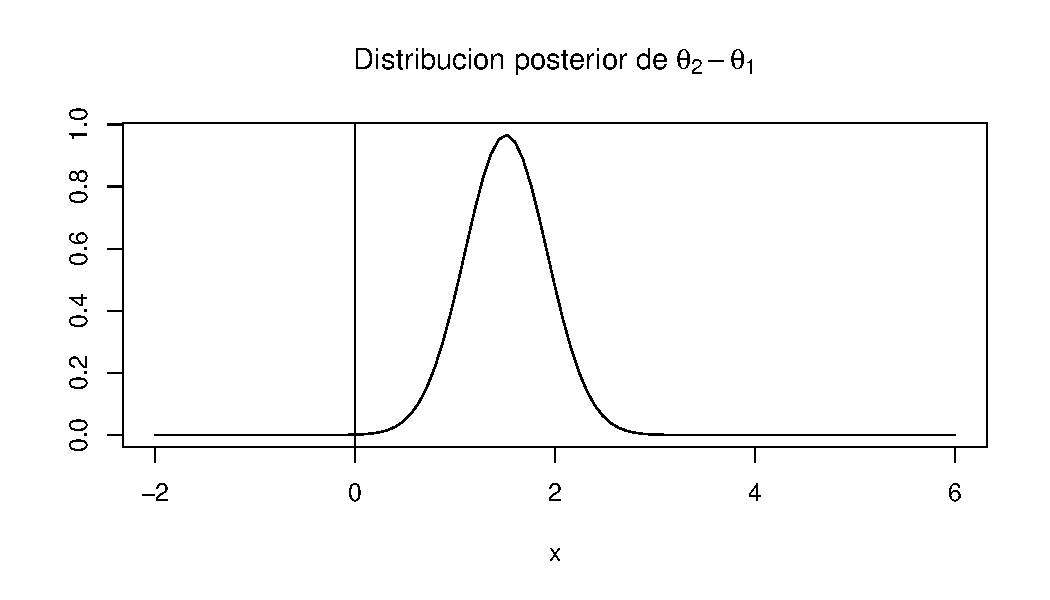
\includegraphics[width=\maxwidth]{figure/unnamed-chunk-44-1} 

\end{knitrout}

De esta forma, podemos concluir que el segundo medicamento tiene un desempe\~no superior al primero.

Finalmente, ilustramos los resultados obtenidos al usar una distribuci\'on previa no informativa, para eso, usaremos $\bGamma=\begin{pmatrix}100&0\\ 0&100\end{pmatrix}$, con $|\bGamma^{-1}|=0.0001$, representando una distribuci\'on previa no informativa. Los resultados de estimaci\'on arroja la siguiente distribuci\'on posterior para el vectro de par\'ametros 
\begin{equation*}
\begin{pmatrix}
\theta_1\\
\theta_2
\end{pmatrix}
\sim N_2\left(\begin{pmatrix}
0.75\\
2.33
\end{pmatrix},\begin{pmatrix}
0.10&0.06\\
0.06&0.20
\end{pmatrix}\right)
\end{equation*}

Los intervalos de credibilidad del 95\% para los par\'ametros $\theta_1$ y $\theta_2$ est\'an dados por $(0.129, 1.368)$ y $(1.451, 3.202)$, respectivamente. Observamos que estos intervalos de credibilidad son muy similares a los intervalos de confianza del 95\% del enfoque cl\'asico\footnote{Estos intervalos de confianza fueron calculados con la expresi\'on $\bar{y}\pm z_{1-\alpha/2}\frac{\sigma}{\sqrt{n}}$} dados por $(0.130, 1.370)$ y $(1.453, 3.207)$. En cuanto a la comparaci\'on entre los dos medicamentos, lo dejamos como ejercicio para los lectores.
\end{Eje}


Finalmente, recordamos los dos siguientes resultados relacionados con la distribuci\'on normal multivariante que pueden resultar \'utiles en otros an\'alisis.
\begin{Res}
La distribuci\'on posterior marginal de un subconjunto de par\'ametros, digamos $\btheta^{(1)}$ es tambi\'en normal multivariante con media igual a la del subvector de medias apropiado, $\bmu_n^{(1)}$ y similar matriz de varianzas $\bGamma_n^{(11)}$.
\end{Res}
  
\begin{Res}
  La distribuci\'on posterior condicional de un subconjunto de par\'ametros, digamos $\btheta^{(1)}$, dado $\btheta^{(2)}$ es tambi\'en normal multivariante dada por
  \begin{equation*}
  \btheta^{(1)} \mid \btheta^{(2)} \sim N_p \left(\bmu_n^{(1)}+\bGamma_n^{(12)}\left(\bGamma_n^{(22)}\right)^{-1}
  \left(\theta^{(2)}-\mu_n^{(2)}\right),\bGamma_n^{(1 \mid 2)}\right).
  \end{equation*}
  En donde
  \begin{align}
  \bGamma_n^{(1 \mid 2)}&= \bGamma_n^{(11)}-\bGamma_n^{(12)}\left(\bGamma_n^{(22)}\right)^{-1}\bGamma_n^{(21)}
  \end{align}

$\bmu^{(1)}$ y $\bmu^{(2)}$ corresponden al vector de medias y $\bGamma_n^{(11)}$, $\bGamma_n^{(22)}$ denotan la matriz de varianzas y covarianzas de $\btheta^{(1)}$ y $\btheta^{(2)}$, respectivamente. $\bGamma_n^{(12)}$ es la matriz de covarianzas entre $\btheta^{(1)}$ y $\btheta^{(2)}$, $\bGamma_n^{(21)}$ es la matriz de covarianzas entre $\btheta^{(2)}$ y $\btheta^{(1)}$. 
\end{Res}
  
La prueba de los dos resultados anteriores se sigue inmediatamente de las propiedades de la distribuci\'on normal multivariante.


\section{Normal multivariante con media y varianza desconocida}
  
Al igual que en la distribuci\'on normal univariada, cuando se desconoce tanto el vector de medias como la matriz de varianzas y covarianzas de la distribuci\'on, es necesario plantear diversos enfoques y situarse en el m\'as conveniente.\footnote{N\'otese que en t\'erminos de par\'ametros, existen $p$ par\'ametros correspondientes al vector de medias $\btheta$ y $\binom{p}{2}=\dfrac{p(p+1)}{2}$ par\'ametros correspondientes a la matriz de varianzas $\bSigma$. Pensando en la gran cantidad de par\'ametros que se deben modelar, es necesario tener en cuenta que el n\'umero de datos en la muestra aleatoria sea lo suficientemente grande.} Suponiendo que el n\'umero de observaciones en la muestra aleatoria sea suficiente, existe otra situaci\'on que se debe surtir y es la asignaci\'on de las distribuciones previas para $\btheta$ y $\bSigma$. En estos t\'erminos, es posible
  
\begin{itemize}
\item Suponer que la distribuci\'on previa $p(\btheta)$ es independiente de la distribuci\'on previa $p(\bSigma)$ y que ambas distribuciones son informativas. Luego, utilizar un an\'alisis de simulaci\'on condicional conjunta para extraer muestras provenientes de las respectivas distribuciones posterior.
\item Suponer que la distribuci\'on previa para $\btheta$ depende de $\bSigma$ y escribirla como $p(\btheta \mid \bSigma)$, mientras que la distribuci\'on previa de $\bSigma$ no depende de $\btheta$ y se puede escribir como $p(\bSigma)$. El an\'alisis posterior de este enfoque encuentra la distribuci\'on posterior de $\bSigma \mid \mathbf{Y}$ y con esta se encuentra la distribuci\'on posterior de $\btheta \mid \bSigma,\mathbf{Y}$.
\item Suponer que la distribuci\'on previa para $\btheta$ y $\bSigma$ es una distribuci\'on no informativas.
\end{itemize}

  
\subsection{Par\'ametros independientes con distribuciones previas informativas}

En este enfoque se supone que las distribuciones previas para los par\'ametros de inter\'es son independientes e informativas. La funci\'on de verosimilitud est\'a dada en la expresi\'on $\ref{Vero_Multi}$. Hacemos siguiente observaci\'on para lograr que las resultantes distribuciones posterior sean conjugadas. 
\begin{align*}
\sum_{i=1}^n(\mathbf{Y}_i-\theta)'\bSigma^{-1}(\mathbf{Y}_i-\theta)&=traza \left(\sum_{i=1}^n(\mathbf{Y}_i-\theta)'\bSigma^{-1}(\mathbf{Y}_i-\theta)\right)\\
&= \sum_{i=1}^ntraza\left((\mathbf{Y}_i-\theta)'\bSigma^{-1}(\mathbf{Y}_i-\theta)\right)\\
&= \sum_{i=1}^ntraza\left(\bSigma^{-1}(\mathbf{Y}_i-\theta)(\mathbf{Y}_i-\theta)'\right)\\
&= traza\left(\bSigma^{-1}\sum_{i=1}^n(\mathbf{Y}_i-\theta)(\mathbf{Y}_i-\theta)'\right)\\
&= traza\left(\bSigma^{-1}\mathbf{S}_{\btheta}\right)
\end{align*}

Donde $\mathbf{S}_{\btheta}=\sum_{i=1}^n(\mathbf{Y}_i-\btheta)(\mathbf{Y}_i-\btheta)'$. En cuanto a la asignaci\'on de las distribuciones previas, para el vector de medias $\btheta$ es posible usar la distribuci\'on normal, esto es,
\begin{equation*}
\btheta \sim Normal_p(\bmu,\bGamma)
\end{equation*}

Por otro lado, la distribuci\'on para la matriz de varianzas $\bSigma$ es
\begin{equation*}
\bSigma \sim Inversa-Wishart(\bLambda,v)
\end{equation*}

donde $v$ denota el grado de libertad y $\bLambda$ la matriz de escala. Esto es, la funci\'on de densidad est\'a dada por
\begin{equation*}
p(\bSigma)\propto |\bSigma|^{-\frac{v+p+1}{2}}\exp\left\{-\frac{1}{2}traza(\bLambda\bSigma^{-1})\right\}
\end{equation*}

Asumiendo independencia previa, la distribuci\'on previa conjunta resulta estar dada por
\begin{align}
p(\btheta,\bSigma)&=p(\btheta)p(\bSigma)\notag\\
&\propto \mid \bSigma \mid ^{-(v+p+1)/2}\notag\\
&\times
\exp\left\{ -\frac{1}{2}\left[traza(\bLambda\bSigma^{-1})+
(\btheta-\bmu)'\bGamma^{-1}(\btheta-\bmu)\right]\right\}
\end{align}


Una vez que se conoce la forma estructural de la distribuci\'on previa conjunta, es posible establecer la distribuci\'on posterior conjunta teniendo en cuenta la forma de la funci\'on de verosimilitud $p(\mathbf{Y} \mid \btheta,\bSigma)$ y la expresi\'on equivalente para $\sum_{i=1}^n(\mathbf{Y}_i-\btheta)'\bSigma^{-1}(\mathbf{Y}_i-\btheta)$ mostrada al inicio de esta secci\'on. Adicionalmente, acudiendo a la simetr\'ia de las matrices $\bLambda$, $\bSigma$ y $\mathbf{S}_{\btheta}$, se tiene que
\begin{align}
p(\btheta,\bSigma \mid \mathbf{Y})&\propto p(\btheta,\bSigma)p(\mathbf{Y} \mid \btheta,\bSigma)\notag\\
&\propto \mid \bSigma \mid ^{-(v+n+p+1)/2}\notag\\
&\times
\exp\left\{ -\frac{1}{2}\left[traza(\bLambda\bSigma^{-1}+\bSigma^{-1}\mathbf{S}_{\btheta})+
                                (\btheta-\bmu)'\bGamma^{-1}(\btheta-\bmu)\right]\right\}\notag\\
                              &\propto \mid \bSigma \mid ^{-(v+n+p+1)/2}\notag\\
                              &\times
                              \exp\left\{ -\frac{1}{2}\left[traza(\bSigma^{-1}(\bLambda+\mathbf{S}_{\btheta}))+
                              (\btheta-\bmu)'\bGamma^{-1}(\btheta-\bmu)\right]\right\}
\end{align}

Dado que la distribuci\'on posterior conjunta no tiene una forma estructural conocida, no es posible utilizar el m\'etodo de integraci\'on anal\'itica. Sin embargo, es posible obtener las distribuciones condicionales de cada uno de los par\'ametros suponiendo fijos los restantes y teniendo en cuenta que
\begin{align*}
p(\btheta \mid \bSigma,\mathbf{Y})\propto p(\btheta,\underbrace{\bSigma}_{fijo} \mid \mathbf{Y})
\ \ \ \ \ \ \ \ \ \text{y} \ \ \ \ \ \ \ \ \ \
p(\bSigma \mid \btheta,\mathbf{Y})\propto p(\underbrace{\btheta}_{fijo},\bSigma \mid \mathbf{Y})
\end{align*}

\begin{Res}
La distribuci\'on posterior de la matriz de par\'ametros $\bSigma$ condicional a $\btheta,\mathbf{Y}$ es
\begin{equation*}\label{Pos_Cond_bSigma}
\bSigma \mid \btheta,\mathbf{Y} \sim Inversa-Wishart_{v+n}(\bLambda+\mathbf{S}_{\btheta})
\end{equation*}
\end{Res}

\begin{proof}
La prueba es inmediata notando que
\begin{align*}
\bSigma \mid \btheta,\mathbf{Y}&\propto\mid \bSigma \mid ^{-(v+n+p+1)/2}\notag\\
&\times\exp\left\{ -\frac{1}{2}\left[traza(\bSigma^{-1}(\bLambda+\mathbf{S}_{\btheta}))+(\btheta-\bmu)'\bGamma^{-1}(\btheta-\bmu)\right]\right\}
\end{align*}

Por lo tanto, factorizando convenientemente, se encuentra una expresi\'on id\'entica a la funci\'on de distribuci\'on de una variable aleatoria con distribuci\'on $Inversa-Wishart_{v+n}(\bLambda+\mathbf{S}_{\btheta})$.
\end{proof}
                          
\begin{Res}
La distribuci\'on posterior del vector de par\'ametros $\btheta$ condicional a $\bSigma,\mathbf{Y}$ es
\begin{equation}\label{Pos_Cond_btheta}
\btheta \mid  \bSigma,\mathbf{Y} \sim Normal_p(\bmu_n,\bGamma_n)
\end{equation}
donde $\bmu_n$ y $\bGamma_n$ est\'an dadas por las expresiones (\ref{Gamma_n}) y (\ref{mu_n}), respectivamente.
\end{Res}
                              
\begin{proof}
La prueba de este resultado es inmediata pues corresponde a la misma situaci\'on de estimar $\btheta$ cuando $\bSigma$ es conocida. 
\end{proof}

Una vez encontradas las distribuciones posteriores condicionales de $\btheta$ y $\bSigma$, se puede obtener la estimaci\'on de estos par\'ametros v\'ia el muestreador de Gibbs, que en este caso se resume en los siguientes pasos:
\begin{enumerate}[(1)]
\item Fijar un valor inicial para $\btheta$, lo denotamos por $\btheta_{(1)}$
\item Simular un valor de la distribuci\'on de $\bSigma|\btheta,\mathbf{Y}$ en \ref{Pos_Cond_bSigma} donde el par\'ametro $\mathbf{S_\mathbf{\btheta}}$ que depende de $\btheta$, debe ser reemplazado por $\btheta_{(1)}$ del paso anterior. Este valor simulado se denotar\'a por $\bSigma_{(1)}$
\item  Simlar un valor de la distribuci\'on de $\btheta|\bSigma,\mathbf{Y}$ en \ref{Pos_Cond_btheta} donde en $\mathbf{mu}_n$ y $\bGamma_n$ se debe reemplazar $\bSigma$ por $\bSigma$. Este valor simulado se denota por $\btheta$.
\item Se repite los pasos (2) y (3) hasta completar un n\'umero de iteraciones suficientes para alcanzar la convergencia en ambos par\'ametros
\end{enumerate}
Una vez tengamos los valores muestreados, se debe garantizar la convergencia y la correlaci\'on nula entre estos valores, con el fin de calcular las estimaciones. En el siguiente ejemplo ilustramos la implementaci\'on de este muestreador de Gibbs en \verb'JAGS' y \verb'R'.

\begin{Eje}\label{Eje_Student_2}
Retomamos los datos del efecto de dos medicamentos sopor\'iferos introducidos por \citeasnoun{Student} que fueron estudiados en el ejemplo \ref{Eje_Student} asumiendo que la matriz de varianzas y covarianzas es conocida. El vector de medias muestrales de estos datos est\'an dados por $\bar{y}=(0.75, 2.33)'$, y la matriz de varianzas y covarianzas muestrales est\'a dada por $\mathbf{S}=\begin{pmatrix}3.20&2.85\\2.85&4.01\end{pmatrix}$. 

Ahora supongamos que tanto el vector de medias como la matriz de varianzas y covarianzas y desconocidos. Para el vectro de medias, asumimos la distribuci\'on previa del ejemplo \ref{Eje_Student}, es decir, $\bmu=(0,1)'$ y $\bGamma=\begin{pmatrix}2&0\\0&2\end{pmatrix}$. Para la matriz de varianzas y covarianzas asumimos la distribuci\'on inversa Wishart con matriz de escala igual a $\bLambda=\begin{pmatrix}20&8\\8&20\end{pmatrix}$ y grado de libertad $v=10$, de esta forma, la estimaci\'on previa de $\bSigma$ viene dada por $\frac{1}{v-2-1}\bLambda=\begin{pmatrix}2.86&1.14\\ 1.14&2.86\end{pmatrix}$. 

Ilustramos los c\'odigos de \verb'JAGS' a continuaci\'on.

\begin{knitrout}
\definecolor{shadecolor}{rgb}{0.933, 0.933, 0.933}\color{fgcolor}\begin{kframe}
\begin{alltt}
\hlkwd{set.seed}\hlstd{(}\hlnum{123456}\hlstd{)}
\hlstd{n} \hlkwb{<-} \hlnum{10}
\hlstd{mu}\hlkwb{<-} \hlkwd{as.vector}\hlstd{(}\hlkwd{c}\hlstd{(}\hlnum{0}\hlstd{,}\hlnum{1}\hlstd{)); Gamma} \hlkwb{<-} \hlkwd{matrix}\hlstd{(}\hlkwd{c}\hlstd{(}\hlnum{2}\hlstd{,}\hlnum{0}\hlstd{,}\hlnum{0}\hlstd{,}\hlnum{2}\hlstd{),}\hlnum{2}\hlstd{,}\hlnum{2}\hlstd{)}
\hlstd{v} \hlkwb{<-} \hlnum{10}\hlstd{; Lambda} \hlkwb{<-} \hlkwd{matrix}\hlstd{(}\hlkwd{c}\hlstd{(}\hlnum{20}\hlstd{,}\hlnum{8}\hlstd{,}\hlnum{8}\hlstd{,}\hlnum{20}\hlstd{),}\hlnum{2}\hlstd{,}\hlnum{2}\hlstd{)}

\hlstd{NormMult2.model} \hlkwb{<-} \hlkwa{function}\hlstd{()\{}
\hlkwa{for}\hlstd{(i} \hlkwa{in} \hlnum{1} \hlopt{:} \hlstd{n)}
\hlstd{\{}
  \hlstd{y[i,} \hlnum{1}\hlopt{:}\hlnum{2}\hlstd{]} \hlopt{~} \hlkwd{dmnorm}\hlstd{(theta[], Tau[,])}
\hlstd{\}}
\hlstd{theta[}\hlnum{1}\hlopt{:}\hlnum{2}\hlstd{]} \hlopt{~} \hlkwd{dmnorm}\hlstd{(mu[], Gamma[,])}
\hlstd{Tau[}\hlnum{1}\hlopt{:}\hlnum{2}\hlstd{,}\hlnum{1}\hlopt{:}\hlnum{2}\hlstd{]} \hlopt{~} \hlkwd{dwish}\hlstd{(Lambda[,] , v)}
\hlstd{Sigma[}\hlnum{1}\hlopt{:}\hlnum{2}\hlstd{,}\hlnum{1}\hlopt{:}\hlnum{2}\hlstd{]} \hlkwb{<-} \hlkwd{inverse}\hlstd{(Tau[,])}
\hlstd{\}}

\hlstd{y} \hlkwb{<-} \hlkwd{structure}\hlstd{(}\hlkwc{.Data} \hlstd{= sleep[,}\hlnum{1}\hlstd{],} \hlkwc{.Dim}\hlstd{=}\hlkwd{c}\hlstd{(}\hlnum{10}\hlstd{,}\hlnum{2}\hlstd{))}

\hlstd{NormMult2.data} \hlkwb{<-} \hlkwd{list}\hlstd{(}\hlstr{"y"}\hlstd{,}\hlstr{"n"}\hlstd{,}\hlstr{"mu"}\hlstd{,}\hlstr{"Gamma"}\hlstd{,} \hlstr{"Lambda"}\hlstd{,}\hlstr{"v"}\hlstd{)}
\hlstd{NormMult2.param} \hlkwb{<-} \hlkwd{c}\hlstd{(}\hlstr{"theta"}\hlstd{,} \hlstr{"Sigma"}\hlstd{)}
\hlstd{NormMult2.inits} \hlkwb{<-} \hlkwa{function}\hlstd{()\{}
\hlkwd{list}\hlstd{(}\hlstr{"theta"}\hlstd{=}\hlkwd{c}\hlstd{(}\hlnum{0}\hlstd{,}\hlnum{0}\hlstd{),}\hlstr{"Tau"}\hlstd{=}\hlkwd{diag}\hlstd{(}\hlkwd{rep}\hlstd{(}\hlnum{1}\hlstd{,}\hlnum{2}\hlstd{)))}
\hlstd{\}}

\hlstd{NormMult2.fit} \hlkwb{<-} \hlkwd{jags}\hlstd{(}\hlkwc{data}\hlstd{=NormMult2.data,} \hlkwc{inits}\hlstd{=NormMult2.inits, NormMult2.param,}
                      \hlkwc{n.iter}\hlstd{=}\hlnum{10000}\hlstd{,} \hlkwc{n.burnin}\hlstd{=}\hlnum{1000}\hlstd{,} \hlkwc{model.file}\hlstd{=NormMult2.model)}

\hlkwd{print}\hlstd{(NormMult2.fit)}
\end{alltt}
\end{kframe}
\end{knitrout}

Con base en los resultados anteriores, podemos ver que la estimaci\'on bayesiana para el n\'umero de horas de sue\~no producidas por los dos medicamentos son 0.29 y 1.74, respectivamente. En cuanto a la estimaci\'on de la matriz de varianzas y covarianzas, \'esta est\'a dada por $\hat{\bSigma}=\begin{pmatrix}3.08&2.2\\2.2&3.63\end{pmatrix}$.

A continuaci\'on se muestran los c\'odigos para implementar el muestreador de Gibbs de forma maual en \verb'R'.

\colorbox{black}{\textcolor{white}{\textbf{c\'odigo R}}}
\begin{knitrout}
\definecolor{shadecolor}{rgb}{0.933, 0.933, 0.933}\color{fgcolor}\begin{kframe}
\begin{alltt}
\hlkwd{library}\hlstd{(MCMCpack)}
\hlkwd{library}\hlstd{(mvtnorm)}
\hlstd{y} \hlkwb{<-} \hlkwd{as.matrix}\hlstd{(}\hlkwd{data.frame}\hlstd{(}\hlkwc{M1}\hlstd{=sleep[}\hlnum{1}\hlopt{:}\hlnum{10}\hlstd{,}\hlnum{1}\hlstd{],} \hlkwc{M2}\hlstd{=sleep[}\hlopt{-}\hlstd{(}\hlnum{1}\hlopt{:}\hlnum{10}\hlstd{),}\hlnum{1}\hlstd{]))}
\hlstd{y.bar} \hlkwb{<-} \hlkwd{colMeans}\hlstd{(y)}
\hlstd{n} \hlkwb{<-} \hlkwd{nrow}\hlstd{(y)}

\hlcom{#parametros previos de theta}
\hlstd{mu}\hlkwb{<-} \hlkwd{as.vector}\hlstd{(}\hlkwd{c}\hlstd{(}\hlnum{0}\hlstd{,}\hlnum{1}\hlstd{)); Gamma} \hlkwb{<-} \hlkwd{matrix}\hlstd{(}\hlkwd{c}\hlstd{(}\hlnum{2}\hlstd{,}\hlnum{0}\hlstd{,}\hlnum{0}\hlstd{,}\hlnum{2}\hlstd{),}\hlnum{2}\hlstd{,}\hlnum{2}\hlstd{)}
\hlcom{#parametros previos de Sigma}
\hlstd{v} \hlkwb{<-} \hlnum{10}
\hlstd{Lambda} \hlkwb{<-} \hlkwd{matrix}\hlstd{(}\hlkwd{c}\hlstd{(}\hlnum{20}\hlstd{,}\hlnum{8}\hlstd{,}\hlnum{8}\hlstd{,}\hlnum{20}\hlstd{),}\hlnum{2}\hlstd{,}\hlnum{2}\hlstd{); Lambda.inv} \hlkwb{<-} \hlkwd{solve}\hlstd{(Lambda)}

\hlstd{nsim} \hlkwb{<-} \hlnum{10000}
\hlstd{theta.pos} \hlkwb{<-} \hlkwd{matrix}\hlstd{(}\hlnum{NA}\hlstd{,nsim,}\hlnum{2}\hlstd{)}
\hlstd{Sigma.pos} \hlkwb{<-} \hlkwd{array}\hlstd{(}\hlnum{NA}\hlstd{,}\hlkwd{c}\hlstd{(nsim,}\hlnum{2}\hlstd{,}\hlnum{2}\hlstd{))}

\hlcom{# Valor inicial de theta}
\hlstd{theta.pos[}\hlnum{1}\hlstd{,]} \hlkwb{<-} \hlkwd{c}\hlstd{(}\hlnum{0}\hlstd{,}\hlnum{1}\hlstd{)}

\hlcom{#parametros posteriores de Sigma}
\hlstd{v.pos} \hlkwb{<-} \hlstd{v} \hlopt{+} \hlstd{n}
\hlstd{matrix.theta} \hlkwb{<-} \hlkwd{kronecker}\hlstd{(}\hlkwd{matrix}\hlstd{(}\hlkwd{rep}\hlstd{(}\hlnum{1}\hlstd{,n)),}\hlkwd{t}\hlstd{(theta.pos[}\hlnum{1}\hlstd{,]))}
\hlstd{S.theta} \hlkwb{<-} \hlkwd{t}\hlstd{(y}\hlopt{-}\hlstd{matrix.theta)} \hlopt \hlstd{(y}\hlopt{-}\hlstd{matrix.theta)}
\hlstd{Lambda.pos} \hlkwb{<-} \hlstd{Lambda} \hlopt{+} \hlstd{S.theta}
\hlcom{#simulacion de la distribucion posterior condicional de Sigma}
\hlstd{Sigma.pos[}\hlnum{1}\hlstd{,,]} \hlkwb{<-} \hlkwd{riwish}\hlstd{(v.pos, Lambda.pos)}

\hlcom{########################}
\hlcom{# Muestreador de Gibbs #}
\hlcom{########################}
\hlkwa{for}\hlstd{(i} \hlkwa{in} \hlnum{2}\hlopt{:}\hlstd{nsim)\{}
  \hlcom{#parametros posteriores de theta	}
  \hlstd{Gamma.n} \hlkwb{<-} \hlkwd{solve}\hlstd{(}\hlkwd{solve}\hlstd{(Gamma)} \hlopt{+} \hlstd{n}\hlopt{*}\hlkwd{solve}\hlstd{(Sigma.pos[i}\hlopt{-}\hlnum{1}\hlstd{,,]))}
  \hlstd{mu.n} \hlkwb{<-} \hlstd{Gamma.n}\hlopt\hlstd{(}\hlkwd{solve}\hlstd{(Gamma)}\hlopt\hlstd{mu} \hlopt{+} \hlstd{n}\hlopt{*}\hlkwd{solve}\hlstd{(Sigma.pos[i}\hlopt{-}\hlnum{1}\hlstd{,,])}\hlopt\hlstd{y.bar)}
  \hlcom{#simulacion de la distribucion posterior condicional de theta}
  \hlstd{theta.pos[i,]} \hlkwb{<-} \hlkwd{rmvnorm}\hlstd{(}\hlnum{1}\hlstd{, mu.n, Gamma.n)}
  \hlcom{#parametros posteriores de Sigma}
  \hlstd{v.pos} \hlkwb{<-} \hlstd{v} \hlopt{+} \hlstd{n}
  \hlstd{matrix.theta} \hlkwb{<-} \hlkwd{kronecker}\hlstd{(}\hlkwd{matrix}\hlstd{(}\hlkwd{rep}\hlstd{(}\hlnum{1}\hlstd{,n)),}\hlkwd{t}\hlstd{(theta.pos[}\hlnum{1}\hlstd{,]))}
  \hlstd{S.theta} \hlkwb{<-} \hlkwd{t}\hlstd{(y}\hlopt{-}\hlstd{matrix.theta)}\hlopt\hlstd{(y}\hlopt{-}\hlstd{matrix.theta)}
  \hlstd{Lambda.pos} \hlkwb{<-} \hlstd{Lambda} \hlopt{+} \hlstd{S.theta}
  \hlcom{#simulacion de la distribucion posterior condicional de Sigma}
  \hlstd{Sigma.pos[i,,]} \hlkwb{<-} \hlkwd{riwish}\hlstd{(v.pos, Lambda.pos)}
\hlstd{\}}
\end{alltt}
\end{kframe}
\end{knitrout}
Una vez finalizada la ejecuci\'on del muestreador de Gibbs, debemos examinar la calidad de los valores muestreados para asegurar que las estimaciones bayesianas sean obtenidas de una muestra de valores que hayan convergido, y en segundo lugar sean aproximadamente incorrelacionados. Para eso a continuaci\'on observamos la gr\'afica de los valores muestreados para algunos par\'ametros (en particular, consideramos los par\'ametros $\theta_1$, $\theta_2$, $\sigma^2_1$ y $\sigma_{12}$), as\'i como la gr\'afica de las autocorrelaciones muestrales.
%<<fig.height=4>>=
%par(mfrow=c(2,2))
%ts.plot(theta.pos[,1]); ts.plot(theta.pos[,2])
%ts.plot(Sigma.pos[,1,1]); ts.plot(Sigma.pos[,2,1])
%acf(theta.pos[,1]); acf(theta.pos[,2])
%acf(Sigma.pos[,1,1]); acf(Sigma.pos[,2,1])
%@
Con estas gr\'aficas, observamos que los valores muestreados han alcanzado la convergencia, adem\'as estos tienen correlaciones cercanas a cero. De esta forma, podemos usar los valores muestreados para calcular las estimaciones y los intervalos de credibilidad.
\begin{knitrout}
\definecolor{shadecolor}{rgb}{0.933, 0.933, 0.933}\color{fgcolor}\begin{kframe}
\begin{alltt}
\hlstd{theta.Bayes} \hlkwb{<-} \hlkwd{colMeans}\hlstd{(theta.pos)}
\hlstd{Sigma.Bayes} \hlkwb{<-} \hlkwd{matrix}\hlstd{(}\hlkwd{c}\hlstd{(}\hlkwd{mean}\hlstd{(Sigma.pos[,}\hlnum{1}\hlstd{,}\hlnum{1}\hlstd{]),} \hlkwd{mean}\hlstd{(Sigma.pos[,}\hlnum{2}\hlstd{,}\hlnum{1}\hlstd{]),}
                        \hlkwd{mean}\hlstd{(Sigma.pos[,}\hlnum{1}\hlstd{,}\hlnum{2}\hlstd{]),} \hlkwd{mean}\hlstd{(Sigma.pos[,}\hlnum{2}\hlstd{,}\hlnum{2}\hlstd{])),}\hlnum{2}\hlstd{,}\hlnum{2}\hlstd{)}
\hlstd{theta.Bayes}
\end{alltt}
\begin{verbatim}
## [1] 0.54 2.04
\end{verbatim}
\begin{alltt}
\hlstd{Sigma.Bayes}
\end{alltt}
\begin{verbatim}
##      [,1] [,2]
## [1,]  3.2  2.6
## [2,]  2.6  4.3
\end{verbatim}
\end{kframe}
\end{knitrout}
El procedimiento inferencial sobre la comparaci\'on entre los efectos de los dos medicamentos se puede realizar de la misma manera como ilustr\'o el ejemplo \ref{Eje_Student}.
\end{Eje}

\subsection{Par\'ametros dependientes}

Al igual que en el caso univariado, la inferencia posterior de los par\'ametros de inter\'es debe ser llevada a cabo en dos etapas: En la primera, se debe establecer la distribuci\'on previa conjunta para ambos par\'ametros mediante
\begin{equation*}
p(\btheta,\bSigma)=p(\bSigma)p(\btheta \mid \bSigma)
\end{equation*}

Luego, en la segunda etapa es posible analizar posterior propiamente cada uno de los par\'ametros de inter\'es puesto que
\begin{equation*}
p(\btheta,\bSigma \mid \mathbf{Y})\propto p(\mathbf{Y} \mid \btheta,\bSigma)p(\btheta,\bSigma)
\end{equation*}

Al igual que en el caso univariado, la anterior formulaci\'on conlleva a asignar una distribuci\'on previa para $\btheta$ dependiente de la matriz $\bSigma$. Esto quiere decir que en la distribuci\'on $p(\btheta \mid \bSigma)$ el valor de $\bSigma$ se considera una constante fija y conocida. Siguiendo los lineamientos de la Secci\'on 3.2, una distribuci\'on previa para $\btheta$  condicional a $\bSigma$ es
\begin{equation*}
p(\btheta \mid \bSigma)\sim Normal_p(\bmu,\bSigma/c_0)
\end{equation*}

Donde $c_0$ es una constante. Por otro lado, y siguiendo los argumentos de la secci\'on anterior, una posible opci\'on para la distribuci\'on previa de $\bSigma$, corresponde a
\begin{equation*}
p(\bSigma)\sim Inversa-Wishart_{v_0}(\bLambda)
\end{equation*}

\begin{Res}
La distribuci\'on previa conjunta de los par\'ametros $\btheta$ y $\bSigma$ est\'a dada por
\begin{equation*}
p(\btheta,\bSigma) \propto \mid \bSigma \mid ^{-(v_0+p)/2-1}
\exp\left\{ -\frac{1}{2}\left[traza(\bLambda_0\bSigma^{-1})+
c_0(\btheta-\bmu)'\bSigma^{-1}(\btheta-\bmu)\right]\right\}
\end{equation*}
\end{Res}
                              
\begin{proof}
La prueba es inmediata al multiplicar las densidades y asignar los t\'erminos que no dependen de los par\'ametros de inter\'es a la constante de proporcionalidad.
\end{proof}
                              
Para encontrar las distribuciones posterior de cada uno de los par\'ametros de inter\'es se utilizan argumentos similares a los de la secci\'on 3.1.2.
                              
\begin{Res}
La distribuci\'on posterior de $\btheta$ condicional a $\bSigma,\mathbf{Y}$ est\'a dada por
\begin{equation*}
\theta \mid \bSigma,\mathbf{Y} \sim Normal_p(\bmu_n,\bSigma/(n+c_0))
\end{equation*}

donde
\begin{equation*}
\mu_n=\frac{n\bar{\mathbf{Y}}+c_0\bmu}{n+c_0}
\end{equation*}
\end{Res}

\begin{proof}
Utilizando propiedades de la distribuci\'on condicional, tenemos que
\begin{align*}
p(\btheta|\bSigma,\mathbf{Y})&\propto p(\btheta, \bSigma|\mathbf{Y})\\
&\propto \mid \bSigma \mid ^{-(v_0+p)/2-1}
\exp\left\{ -\frac{1}{2}\left[traza(\bLambda_0\bSigma^{-1})+
c_0(\btheta-\bmu)'\bSigma^{-1}(\btheta-\bmu)\right]\right\}\\
&\ \ \ \ \ \ \ \ \mid \bSigma \mid ^{-n/2}\exp\left\{-\frac{1}{2}\sum_{i=1}^n(\mathbf{y}_i-\btheta)'\bSigma^{-1}(\mathbf{y}_i-\btheta)\right\}\\
&\propto \exp\left\{ -\frac{1}{2}
c_0(\btheta-\bmu)'\bSigma^{-1}(\btheta-\bmu)\right\}\exp\left\{-\frac{1}{2}\sum_{i=1}^n(\mathbf{y}_i-\btheta)'\bSigma^{-1}(\mathbf{y}_i-\btheta)\right\}
\end{align*}

La anterior expresi\'on es la misma de $p(\btheta\mid\bSigma,\mathbf{Y})$ del resulado \ref{res_mu_n} donde $\bSigma/c_0$ toma el valor de $\bGamma$. as\'i, teniendo en cuenta las ecuaciones (\ref{Gamma_n}) y (\ref{mu_n}), podemos afirmar que el vector de medias y la matriz de varianzas y covarianzas posterior est\'an dadas por
\begin{align}
\bGamma_n&=((\bSigma/c_0)^{-1}+n\bSigma^{-1})^{-1}=\frac{\bSigma}{n+c_0}\\
\bmu_n&=\frac{\bSigma}{n+c_0}((\bSigma/c_0)^{-1}\bmu+n\bSigma^{-1}\bar{\mathbf{y}})=\frac{n\bar{\mathbf{Y}}+c_0\bmu}{n+c_0}
\end{align}
\end{proof}

En cuanto a la distribuci\'on de $\bSigma$, se tiene el siguiente resultado: 
\begin{Res}\label{Pos_Sigma}
La distribuci\'on marginal posterior de la matriz de par\'ametros $\bSigma$ es
\begin{equation*}
\bSigma \mid \mathbf{Y} \sim Inversa-Whishart_{n+v_0}(\bLambda_n)
\end{equation*}

Donde
\begin{equation}\label{bLambda_n}
\bLambda_n=\bLambda+(n-1)\mathbf{S}+\frac{c_0n}{c_0+n}(\bmu-\bar{\mathbf{y}})(\bmu-\bar{\mathbf{y}})'
\end{equation}

con $S$ la matriz de varianzas y covarianzas muestrales.
\end{Res}

\begin{proof}
\begin{align*}
&\ \ \ \ \ p(\bSigma\mid\mathbf{Y})\\
&=\int_{R^p} p(\btheta,\bSigma\mid\mathbf{Y})d\btheta\\
&\propto \int_{R^p}\mid\bSigma\mid^{-(v_0+p+n)/2-1}\exp\left\{-\frac{1}{2}\left[traza(\bLambda\bSigma^{-1})+c_0(\btheta-\bmu)'\bSigma^{-1}(\btheta-\bmu)+\sum_{i=1}^n(\mathbf{y}_i-\btheta)'\bSigma^{-1}(\mathbf{y}_i-\btheta)\right]\right\}d\btheta\\
&\propto \mid\bSigma\mid^{-(v_0+p+n)/2-1} \exp\left\{-\frac{1}{2}\left[traza(\bLambda\bSigma^{-1})\right]\right\}\\
&\ \ \ \ \ \ \ \ \ \ \int_{R^p}\exp\left\{-\frac{1}{2}\left[c_0(\btheta-\bmu)'\bSigma^{-1}(\btheta-\bmu)+\sum_{i=1}^n(\mathbf{y}_i-\btheta)'\bSigma^{-1}(\mathbf{y}_i-\btheta)\right]\right\}d\btheta\\
&\propto \mid\bSigma\mid^{-(v_0+p+n)/2-1} \exp\left\{-\frac{1}{2}\left[traza(\bLambda\bSigma^{-1})+c_0\bmu'\bSigma^{-1}\bmu+\sum_{i=1}^n(\mathbf{y}_i-\bar{\mathbf{y}})'\bSigma^{-1}(\mathbf{y}_i-\bar{\mathbf{y}})+n\bar{\mathbf{y}}'\bSigma^{-1}\bar{\mathbf{y}}\right]\right\}\\
&\ \ \ \ \ \ \ \ \ \ \int_{R^p}\exp\left\{-\frac{1}{2}\left[c_0\btheta'\bSigma^{-1}\btheta-2c_0\bmu'\bSigma^{-1}\btheta-2n\bar{\mathbf{y}}'\bSigma^{-1}\btheta+n\btheta'\bSigma^{-1}\btheta\right]\right\}d\btheta\\
&\propto \mid\bSigma\mid^{-(v_0+p+n)/2-1} \exp\left\{-\frac{1}{2}\left[traza\left((\bLambda+c_0\bmu\bmu'+\sum_{i=1}^n(\mathbf{y}_i-\bar{\mathbf{y}})(\mathbf{y}_i-\bar{\mathbf{y}})'+n\bar{\mathbf{y}}\bar{\mathbf{y}}')\bSigma^{-1}\right)\right]\right\}\\
&\ \ \ \mid\frac{\bSigma}{c_0+n}\mid^{1/2}\exp\left\{\frac{1}{2}\frac{c_0\bmu'+n\bar{\mathbf{y}}'}{c_0+n}\left(\frac{\bSigma}{c_0+n}\right)^{-1}\frac{c_0\bmu+n\bar{\mathbf{y}}}{c_0+n}\right\}\\
&\ \ \ \ \ \ \ \underbrace{\int_{R^p}\mid\frac{\bSigma}{c_0+n}\mid^{-1/2}\exp\left\{-\frac{1}{2}\left(\btheta-\frac{c_0\bmu+n\bar{\mathbf{y}}}{c_0+n}\right)'\left(\frac{\bSigma}{c_0+n}\right)^{-1}\left(\btheta-\frac{c_0\bmu+n\bar{\mathbf{y}}}{c_0+n}\right)\right\}d\btheta}_{\text{Igual a 1}}
\end{align*}

Por otro lado, 
\begin{align*}
&\ \ \ \ \frac{c_0\bmu'+n\bar{\mathbf{y}}'}{c_0+n}\left(\frac{\bSigma}{c_0+n}\right)^{-1}\frac{c_0\bmu+n\bar{\mathbf{y}}}{c_0+n}\\
&=\frac{1}{c_0+n}(c_0\bmu'+n\bar{\mathbf{y}}')\bSigma^{-1}(c_0\bmu+n\bar{\mathbf{y}})\\
&=traza\left(\frac{1}{c_0+n}(c_0\bmu+n\bar{\mathbf{y}})(c_0\bmu'+n\bar{\mathbf{y}}')\bSigma^{-1}\right)\\
&=traza\left(\left(\frac{c_0^2\bmu\bmu'}{c_0+n}+\frac{2c_0n\bar{\mathbf{y}}\bmu'}{c_0+n}+\frac{n^2\bar{\mathbf{y}}\bar{\mathbf{y}}'}{c_0+n}\right)\bSigma^{-1}\right)
\end{align*}

Reemplazando la anterior expresi\'on en $p(\bSigma\mid\mathbf{Y})$, se tiene que
\begin{align*}
&\ \ \ \ \ p(\bSigma\mid\mathbf{Y})\\
&\propto \mid\bSigma\mid^{-(v_0+p+n+1)/2}\exp\left\{-\frac{1}{2}traza\left[\left(\bLambda+(n-1)\mathbf{S}+\frac{c_0n}{c_0+n}(\bmu-\bar{\mathbf{y}})(\bmu-\bar{\mathbf{y}})'\right)\bSigma^{-1}\right]\right\}
\end{align*}

la cual corresponde a la distribuci\'on deseada.
\end{proof}

En t\'erminos de simulaci\'on de densidades, para obtener las estimaciones bayesians de $\btheta$ y $\bSigma$ se debe primero simular valores de $\bSigma$ de la distribuci\'on $p(\bSigma \mid \mathbf{Y})$ y luego, se debe utilizar estos valores para simular valores de $\btheta$ de la distribuci\'on $p(\btheta \mid \bSigma,\mathbf{Y})$.

Una forma equivalente de obtener las estimaciones es calcular directamente la esperanza te\'orica de las distribuciones posteriores marginales de $\btheta$ y de $\bSigma$. 

Del resultado \ref{Pos_Sigma}, podemos concluir que la estimaci\'on bayesiana de la matriz de varianza y covarianzas $\bSigma$ est\'a dada por
\begin{equation*}
\hat{\bSigma}=\dfrac{\bLambda+(n-1)\mathbf{S}+\frac{c_0n}{c_0+n}(\bmu-\bar{\mathbf{y}})(\bmu-\bar{\mathbf{y}})'}{n+v_0-p-1}
\end{equation*}

Teniendo en cuenta que la estimaci\'on previa de $\bSigma$ viene dada por $\hat{\bSigma}_{pre}=\frac{\bLambda}{v_0-p-1}$, podemos ver que la estimaci\'on bayesiana de $\bSigma$ est\'a conformada por tres componentes: la estimaci\'on previa $\hat{\bSigma}_{pre}$, la estimaci\'on cl\'asica $\mathbf{S}$ y una medida de discrepancia entre la estimaci\'on previa y la cl\'asica de $\btheta$. Para encontrar correctas formas de escoger los par\'ametros previas de $\bSigma$, por ahora ignoramos el \'ultimo componente, y vemos que la estimaci\'on previa $\hat{\bSigma}_{pre}$ y la estimaci\'on cl\'asica $\mathbf{S}$ entran al c\'omputo de la estimaci\'on bayesiana con los pesos de $v_0-p-1$ y $n-1$, de esta forma, podemos escoger $v_0$ tal que $v_0-p$ represente el n\'umero de la informaci\'on previa, y el valor de $\bLambda$ se puede calcular a partir de $v_0$ y $\hat{\bSigma}_{pre}$. 

El siguiente resultado muestra la distribuci\'on posterior marginal de $\btheta$. 
                              
\begin{Res}\label{Pos_btheta}
La distribuci\'on marginal posterior del par\'ametro $\btheta$ es la distribuci\'on $t$ de Student multivariante tal que
\begin{equation*}
\btheta \mid \mathbf{Y} \sim t_{n+v_0-p+1}\left(\bmu_n, \frac{\bLambda_n}{(c_0+n)(n+v_0-p+1)}\right)
\end{equation*}

con $\bmu_n=\frac{c_0\bmu+n\bar{\mathbf{y}}}{c_0+n}$ y $\bLambda_n$ dado en la ecuaci\'on (\ref{bLambda_n}).
\end{Res}

\begin{proof}
\begin{align*}
&\ \ \ \ p(\btheta\mid\mathbf{Y})\\
&=\int_{R^p\times R^p}p(\btheta,\bSigma\mid\mathbf{Y})d\bSigma\\
&=\int_{R^p\times R^p} \mid\bSigma\mid^{-(v_0+p+n)/2-1}\exp\left\{-\frac{1}{2}\left[traza(\bLambda\bSigma^{-1})+c_0(\btheta-\bmu)'\bSigma^{-1}(\btheta-\bmu)+\sum_{i=1}^n(\mathbf{y}_i-\btheta)'\bSigma^{-1}(\mathbf{y}_i-\btheta)\right]\right\}d\bSigma\\
&=\int_{R^p\times R^p} \mid\bSigma\mid^{-(v_0+p+n+2)/2}\exp\left\{-\frac{1}{2}traza\left[\bLambda+c_0(\btheta-\bmu)(\btheta-\bmu)'+\sum_{i=1}^n(\mathbf{y}_i-\btheta)(\mathbf{y}_i-\btheta)'\right]\bSigma^{-1}\right\}d\bSigma\\
&\propto \big|\bLambda+c_0(\btheta-\bmu)(\btheta-\bmu)'+\sum_{i=1}^n(\mathbf{y}_i-\btheta)(\mathbf{y}_i-\btheta)'\big|^{-\frac{v_0+n+1}{2}}\\
&=\big|\bLambda+c_0(\btheta-\bmu)(\btheta-\bmu)'+\sum_{i=1}^n(\mathbf{y}_i-\bar{\mathbf{y}})(\mathbf{y}_i-\bar{\mathbf{y}})'+n(\bar{\mathbf{y}}-\btheta)(\bar{\mathbf{y}}-\btheta)'\big|^{-\frac{v_0+n+1}{2}}\\
&=\big|\bLambda+(n-1)\mathbf{S}+\frac{c_0n}{c_0+n}(\bmu-\bar{\mathbf{y}})(\bmu-\bar{\mathbf{y}})'+(c_0+n)(\btheta-\bmu_n)(\btheta-\bmu_n)'\big|^{-\frac{v_0+n+1}{2}}\\
&=\big|\bLambda_n+(c_0+n)(\btheta-\bmu_n)(\btheta-\bmu_n)'\big|^{-\frac{v_0+n+1}{2}}\\
&\propto\big|\mathbf{I}_p+(c_0+n)\bLambda_n^{-1}(\btheta-\bmu_n)(\btheta-\bmu_n)'\big|^{-\frac{v_0+n+1}{2}}\\
&=\big|1+(c_0+n)(\btheta-\bmu_n)'\bLambda_n^{-1}(\btheta-\bmu_n)\big|^{-\frac{v_0+n+1}{2}}\\
&=\big|1+\frac{1}{n+v_0-p+1}(\btheta-\bmu_n)'\left(\frac{\bLambda_n}{(c_0+n)(n+v_0-p+1)}\right)^{-1}(\btheta-\bmu_n)\big|^{-\frac{v_0+n+1}{2}}
\end{align*}

Esta expresi\'on obtenida corresponde a la forma de la distribuci\'on $t$ de Student multivariado. En el desarrollo se utiliz\'o la propiedad $|\mathbf{I}+\mathbf{A}\mathbf{B}|=|\mathbf{I}+\mathbf{B}\mathbf{A}|$ para matrices $\mathbf{A}$ y $\mathbf{B}$ de tama\~nos compatibles para las multiplicaciones. 
\end{proof}

El anterior resultado indica que la estimaci\'on bayesiana del par\'ametro $\btheta$ est\'a dada por 
\begin{equation*}
\hat{\btheta}=\mathbf{\mu}_n=\dfrac{n\hat{\mathbf{Y}}+c_0\mathbf{\mu}}{n+c_0}=\dfrac{n}{n+c_0}\hat{\mathbf{Y}}+\dfrac{c_0}{n+c_0}\mathbf{\mu}
\end{equation*}

donde se puede observar que $\hat{\btheta}$ se acercar\'a a la estimaci\'on cl\'asica $\hat{\mathbf{y}}$ cuando $n$ es grande comparado a $c_0$, de lo contrario se acercar\'a a la estimaci\'on previa $\mathbf{\mu}$. La varianza posterior para el $i$-\'esimo componente de $\btheta$ est\'a dada por 
\begin{equation*}
var(\theta_i|\mathbf{Y})=\dfrac{\lambda_{ii}}{(c_0+n)(n+v_0-p+1)}\dfrac{n+c_0-p+1}{n+c_0-p-1}\approx\dfrac{\lambda_{ii}}{(c_0+n)(n+v_0-p+1)}
\end{equation*}

donde $\lambda_{ii}$ denota el $i$-\'esimo elemento en la diagonal de la matriz $\bLambda_n$.

\begin{Eje}
\citeasnoun{Pena2002} reporta las mediciones de 6 variables indicadoras de desarrollo en 91 paises en los a\~nos noventa. Para este ejemplo, utilizamos tres variables: tasa de natalidad, tasa de mortalidad y mortalidad infantil en algunos paises de Suram\'erica y Asia mostrados en la tabla \ref{Natalidad}. espec\'ificamente, usaresmos los datos de los paises de Suram\'erica como datos muestrales y los de Asia para extraer la informaci\'on previa.
\begin{table}[!htb]\centering
\begin{tabular}{cccc}\hline
Pa\'is&Tasa Nat.&Tasa Mort.&Mort. Inf\\\hline
Argentina&20.7&8.4&25.7\\
Bolivia&46.6&18&111\\
Brasil&28.6&7.9&63\\
Chile&23.4&5.8&17.1\\
Colombia&27.4&6.1&40\\
Ecuador&32.9&7.4&63\\
M\'exico&29&23.2&43\\
Paraguay&34.8&6.6&42\\
Per\'u&32.9&8.3&109.9\\
Uruguay&18&9.6&21.9\\
Venezuela&27.5&4.4&23.3\\
China&21.2&6.7&32\\
India&30.5&10.2&91\\
Indonesia&28.6&9.4&75\\
Malasia&31.6&5.6&24\\
Mongolia&36.1&8.8&68\\
Nepal&39.6&14.8&128\\
Singapur&17.8&5.2&7.5\\\hline
\end{tabular}
\caption{Tasa de natalidad, tasa de mortalidad, mortalidad infantil en algunos pa\'ises}\label{Natalidad}
\end{table}

\begin{knitrout}
\definecolor{shadecolor}{rgb}{0.933, 0.933, 0.933}\color{fgcolor}\begin{kframe}
\begin{alltt}
\hlcom{# Datos muestrales}
\hlstd{y.sam} \hlkwb{<-} \hlkwd{data.frame}\hlstd{(}\hlkwc{Nat}\hlstd{=}\hlkwd{c}\hlstd{(}\hlnum{20.7}\hlstd{,}\hlnum{46.6}\hlstd{,} \hlnum{28.6}\hlstd{,}\hlnum{23.4}\hlstd{,}\hlnum{27.4}\hlstd{,}\hlnum{32.9}\hlstd{,}\hlnum{29}\hlstd{,}\hlnum{34.8}\hlstd{,}\hlnum{32.9}\hlstd{,}\hlnum{18}\hlstd{,}\hlnum{27.5}\hlstd{),}
             \hlkwc{Mort}\hlstd{=}\hlkwd{c}\hlstd{(}\hlnum{8.4}\hlstd{,}\hlnum{18}\hlstd{,}\hlnum{7.9}\hlstd{,}\hlnum{5.8}\hlstd{,}\hlnum{6.1}\hlstd{,}\hlnum{7.4}\hlstd{,}\hlnum{23.2}\hlstd{,}\hlnum{6.6}\hlstd{,}\hlnum{8.3}\hlstd{,}\hlnum{9.6}\hlstd{,}\hlnum{4.4}\hlstd{),}
                \hlkwc{Infa}\hlstd{=}\hlkwd{c}\hlstd{(}\hlnum{25.7}\hlstd{,}\hlnum{111}\hlstd{,}\hlnum{63}\hlstd{,}\hlnum{17.1}\hlstd{,}\hlnum{40}\hlstd{,}\hlnum{63}\hlstd{,}\hlnum{43}\hlstd{,}\hlnum{42}\hlstd{,}\hlnum{109.9}\hlstd{,}\hlnum{21.9}\hlstd{,}\hlnum{23.3}\hlstd{))}
\hlcom{# Datos de la informacion previa}
\hlstd{y.pre} \hlkwb{<-} \hlkwd{data.frame}\hlstd{(}\hlkwc{Nat}\hlstd{=}\hlkwd{c}\hlstd{(}\hlnum{21.2}\hlstd{,}\hlnum{30.5}\hlstd{,}\hlnum{28.6}\hlstd{,}\hlnum{31.6}\hlstd{,}\hlnum{36.1}\hlstd{,}\hlnum{39.6}\hlstd{,}\hlnum{17.8}\hlstd{),}
                         \hlkwc{Mort}\hlstd{=}\hlkwd{c}\hlstd{(}\hlnum{6.7}\hlstd{,}\hlnum{10.2}\hlstd{,}\hlnum{9.4}\hlstd{,}\hlnum{5.6}\hlstd{,}\hlnum{8.8}\hlstd{,}\hlnum{14.8}\hlstd{,}\hlnum{5.2}\hlstd{),}
                            \hlkwc{Infa}\hlstd{=}\hlkwd{c}\hlstd{(}\hlnum{32}\hlstd{,}\hlnum{91}\hlstd{,}\hlnum{75}\hlstd{,}\hlnum{24}\hlstd{,}\hlnum{68}\hlstd{,}\hlnum{128}\hlstd{,}\hlnum{7.5}\hlstd{))}
\hlstd{p} \hlkwb{<-} \hlkwd{ncol}\hlstd{(y.pre)}
\hlcom{# Estimacion clasica de los parametros}
\hlstd{y.bar} \hlkwb{<-} \hlkwd{colMeans}\hlstd{(y.sam); S} \hlkwb{<-} \hlkwd{var}\hlstd{(y.sam); n} \hlkwb{<-} \hlkwd{nrow}\hlstd{(y.sam)}
\hlcom{# Estimacion previa de los parametros}
\hlstd{mu} \hlkwb{<-} \hlkwd{colMeans}\hlstd{(y.pre); c0} \hlkwb{<-} \hlkwd{nrow}\hlstd{(y.pre)}
\hlstd{v0} \hlkwb{<-} \hlstd{p} \hlopt{+} \hlkwd{nrow}\hlstd{(y.pre); Lambda} \hlkwb{<-} \hlkwd{var}\hlstd{(y.pre)}\hlopt{*}\hlstd{(v0}\hlopt{-}\hlstd{p}\hlopt{-}\hlnum{1}\hlstd{)}
\hlcom{# parametro de las distribuciones posteriores marginales}
\hlstd{mu.n} \hlkwb{<-} \hlstd{(n}\hlopt{*}\hlstd{y.bar} \hlopt{+} \hlstd{c0}\hlopt{*}\hlstd{mu)}\hlopt{/}\hlstd{(n}\hlopt{+}\hlstd{c0)}
\hlstd{Lambda.n} \hlkwb{<-} \hlstd{Lambda} \hlopt{+} \hlstd{(n}\hlopt{-}\hlnum{1}\hlstd{)}\hlopt{*}\hlstd{S} \hlopt{+} \hlkwd{matrix}\hlstd{(mu}\hlopt{-}\hlstd{y.bar)}\hlopt\hlkwd{t}\hlstd{(}\hlkwd{matrix}\hlstd{(mu}\hlopt{-}\hlstd{y.bar))}\hlopt{*}\hlstd{c0}\hlopt{*}\hlstd{n}
\hlstd{var.theta} \hlkwb{<-} \hlstd{Lambda.n}\hlopt{/}\hlstd{((c0}\hlopt{+}\hlstd{n)}\hlopt{*}\hlstd{(n}\hlopt{+}\hlstd{v0}\hlopt{-}\hlstd{p}\hlopt{+}\hlnum{1}\hlstd{))}
\hlstd{mu.n}
\end{alltt}
\begin{verbatim}
##  Nat Mort Infa 
## 29.3  9.2 54.7
\end{verbatim}
\begin{alltt}
\hlstd{var.theta}
\end{alltt}
\begin{verbatim}
##        Nat Mort Infa
## Nat   2.80 0.79 10.7
## Mort  0.79 1.35  2.2
## Infa 10.68 2.20 85.5
\end{verbatim}
\begin{alltt}
\hlstd{Lambda.n}
\end{alltt}
\begin{verbatim}
##       Nat Mort  Infa
## Nat   957  270  3651
## Mort  270  463   751
## Infa 3651  751 29257
\end{verbatim}
\end{kframe}
\end{knitrout}

De los anteriores c\'alculos, se puede ver que la distribuci\'on posterior de $\btheta$ est\'a dada por
\begin{equation*}
\btheta\mid\mathbf{Y}\sim t_{19}\left(\begin{pmatrix}29.3\\9.2\\54.7\end{pmatrix}, \begin{pmatrix}2.80&0.79&10.68\\0.79&1.35&2.20\\10.68&2.20&85.55\end{pmatrix}\right)
\end{equation*}

Usando propiedades de la distribuci\'on multivariante $t$ de Student, tenemos que $\theta_1\sim t_{19}(29.29, 2.80)$, $\theta_2\sim t_{19}(9.24, 1.35)$ y $\theta_3\sim t_{19}(0.62, 85.55)$, de all\'i se puede encontrar f\'acilmente los intervalos de credibilidad para cada uno de estos tres par\'ametros.

En cuanto a la distribuci\'on posterior de $\bSigma$, \'esta est\'a dada por
\begin{equation*}
\bSigma\mid\mathbf{Y}\sim Inversa-Wishart_{21}\left(\begin{pmatrix}957&270&3651\\ 270&463&751\\ 3651&751&29257\end{pmatrix}\right)
\end{equation*}

y la estimaci\'on bayesiana de $\bSigma$ viene dada por $\hat{\bSigma}=\begin{pmatrix}56.3&15.9&214.8\\15.9&27.2&44.2\\214.8&44.2&1721.0\end{pmatrix}$. Por propiedad de la distribuci\'on inversa-Wishart, se puede concluir que los elementos diagonales de $\bSigma$ tienen distribuci\'on inversa-Gamma. Por ejemplo, se tiene que $\sigma^2_{1}\sim Inversa-Gamma(21/2, 56.3/2)$ y cualquier inferencia que se desear realizar sobre $\sigma^2_{1}$ es posible a partir de esta distribuci\'on. 

Aparte de los an\'alisis anteriores, tambi\'en podemos realizar ejercicios de comparaci\'on y verificar posible independencia entre parejas de variables. Por ejemplo, queremos verificar la hip\'ostesis de que la tasa de natalidad es dos veces la tasa de mortalidad, esto es $\theta_1=2\theta_2$. Una forma de confirmar o refutar esta hip\'otesis es hallar el intervalo de credibilidad del $\theta_1-2\theta_2$ que se puede expresar como $(1,-2,0)\begin{pmatrix}\theta_1\\ \theta_2\\ \theta_3\end{pmatrix}$. Por propiedad de la distribuci\'on $t$ de Student multivariante, tenemos que $\theta_1-2\theta_2$ tiene distribuci\'on $t$ de Student univariada con el mismo grado de libertad que $\btheta$, la esperanza est\'a dada por $(1,-2,0)\begin{pmatrix}29.3\\9.2\\54.7\end{pmatrix}=10.8$ y la escala est\'a dada por $(1,-2,0)\begin{pmatrix}2.80&0.79&10.68\\0.79&1.35&2.20\\10.68&2.20&85.55\end{pmatrix}\begin{pmatrix}1\\-2\\0\end{pmatrix}=5.054$, esto es, 
\begin{equation*}
\theta_1-2\theta_2 \mid \mathbf{Y}\sim t_{19}(10.8, 5.054)
\end{equation*}

De esta forma, un intervalo de credibilidad para $\theta_1-2\theta_2$ viene dado por los percentiles 2.5\% y 97.5\% de la anterior distribuci\'on, que a la vez son iguales a los percentiles 2.5\% y 97.5\% de la distribuci\'on $t$ de Student estandarizada multiplicado por $\sqrt{5.054}$ y sumado 10.8. Este invervalo es igual a $(6.095, 15.505)$. Al observar que este intervalo no contiene el valor 0, podemos concluir que no es v\'alido afirmar que la tasa de natalidad sea dos veces la tasa de mortalidad.

En el anterior an\'alisis, vemos que el intervalo de crediblidad para $\theta_1-2\theta_2$ contiene solo valores positivos, lo cual es un indicio de que la variable $\theta_1-2\theta_2$ tenga la mayor parte de la funci\'on de densidad ubicado en ele eje positivo. He hecho podemos indagar $Pr(\theta_1-2\theta_2>0)$, esto lo podemos calcular de la distribuci\'on $t_{19}(10.8, 5.054)$ encontrada anteriormente. Esta probabilidad se puede calcular usando \verb'1-pt((0-10.8)/sqrt(5.054),19)' dando como resultado 0.9999383, de donde muestra una fuerte evidencia de que la tasa de natalidad es superior a dos veces la tasa de mortalidad.

Los anteriores resultados fueron obtenidos directamente de las distribuciones posteriores marginales $p(\btheta|\mathbf{Y})$ y $p(\bSigma|\mathbf{Y})$. De forma equivalente tambi\'en se puede usar las t\'ecnicas de simulaci\'on con base en las distribuciones $p(\btheta,\bSigma|\mathbf{Y})$ y $p(\bSigma|\mathbf{Y})$. A continuaci\'on se muestra los c\'odigos:
\begin{knitrout}
\definecolor{shadecolor}{rgb}{0.933, 0.933, 0.933}\color{fgcolor}\begin{kframe}
\begin{alltt}
\hlkwd{library}\hlstd{(MCMCpack)}
\hlkwd{library}\hlstd{(mvtnorm)}
\hlcom{# Datos muestrales}
\hlstd{y.sam} \hlkwb{<-} \hlkwd{data.frame}\hlstd{(}\hlkwc{Nat}\hlstd{=}\hlkwd{c}\hlstd{(}\hlnum{20.7}\hlstd{,}\hlnum{46.6}\hlstd{,} \hlnum{28.6}\hlstd{,}\hlnum{23.4}\hlstd{,}\hlnum{27.4}\hlstd{,}\hlnum{32.9}\hlstd{,}\hlnum{29}\hlstd{,}\hlnum{34.8}\hlstd{,}\hlnum{32.9}\hlstd{,}\hlnum{18}\hlstd{,}\hlnum{27.5}\hlstd{),}
             \hlkwc{Mort}\hlstd{=}\hlkwd{c}\hlstd{(}\hlnum{8.4}\hlstd{,}\hlnum{18}\hlstd{,}\hlnum{7.9}\hlstd{,}\hlnum{5.8}\hlstd{,}\hlnum{6.1}\hlstd{,}\hlnum{7.4}\hlstd{,}\hlnum{23.2}\hlstd{,}\hlnum{6.6}\hlstd{,}\hlnum{8.3}\hlstd{,}\hlnum{9.6}\hlstd{,}\hlnum{4.4}\hlstd{),}
                \hlkwc{Infa}\hlstd{=}\hlkwd{c}\hlstd{(}\hlnum{25.7}\hlstd{,}\hlnum{111}\hlstd{,}\hlnum{63}\hlstd{,}\hlnum{17.1}\hlstd{,}\hlnum{40}\hlstd{,}\hlnum{63}\hlstd{,}\hlnum{43}\hlstd{,}\hlnum{42}\hlstd{,}\hlnum{109.9}\hlstd{,}\hlnum{21.9}\hlstd{,}\hlnum{23.3}\hlstd{))}
\hlcom{# Datos de la informaci\textbackslash{}'on previa}
\hlstd{y.pre} \hlkwb{<-} \hlkwd{data.frame}\hlstd{(}\hlkwc{Nat}\hlstd{=}\hlkwd{c}\hlstd{(}\hlnum{21.2}\hlstd{,}\hlnum{30.5}\hlstd{,}\hlnum{28.6}\hlstd{,}\hlnum{31.6}\hlstd{,}\hlnum{36.1}\hlstd{,}\hlnum{39.6}\hlstd{,}\hlnum{17.8}\hlstd{),}
                        \hlkwc{Mort}\hlstd{=}\hlkwd{c}\hlstd{(}\hlnum{6.7}\hlstd{,}\hlnum{10.2}\hlstd{,}\hlnum{9.4}\hlstd{,}\hlnum{5.6}\hlstd{,}\hlnum{8.8}\hlstd{,}\hlnum{14.8}\hlstd{,}\hlnum{5.2}\hlstd{),}
                           \hlkwc{Infa}\hlstd{=}\hlkwd{c}\hlstd{(}\hlnum{32}\hlstd{,}\hlnum{91}\hlstd{,}\hlnum{75}\hlstd{,}\hlnum{24}\hlstd{,}\hlnum{68}\hlstd{,}\hlnum{128}\hlstd{,}\hlnum{7.5}\hlstd{))}
\hlstd{p} \hlkwb{<-} \hlkwd{ncol}\hlstd{(y.pre)}
\hlcom{# Estimacion clasica de los parametros}
\hlstd{y.bar} \hlkwb{<-} \hlkwd{colMeans}\hlstd{(y.sam); S} \hlkwb{<-} \hlkwd{var}\hlstd{(y.sam); n} \hlkwb{<-} \hlkwd{nrow}\hlstd{(y.sam)}
\hlcom{# Estimacion previa de los parametros}
\hlstd{mu} \hlkwb{<-} \hlkwd{colMeans}\hlstd{(y.pre); c0} \hlkwb{<-} \hlkwd{nrow}\hlstd{(y.pre)}
\hlstd{v0} \hlkwb{<-} \hlstd{p} \hlopt{+} \hlkwd{nrow}\hlstd{(y.pre); Lambda} \hlkwb{<-} \hlkwd{var}\hlstd{(y.pre)}\hlopt{*}\hlstd{(v0}\hlopt{-}\hlstd{p}\hlopt{-}\hlnum{1}\hlstd{)}
\hlcom{# parametros de las posteriores}
\hlstd{Lambda.n} \hlkwb{<-} \hlstd{Lambda} \hlopt{+} \hlstd{(n}\hlopt{-}\hlnum{1}\hlstd{)}\hlopt{*}\hlstd{S} \hlopt{+} \hlkwd{matrix}\hlstd{(mu}\hlopt{-}\hlstd{y.bar)}\hlopt\hlkwd{t}\hlstd{(}\hlkwd{matrix}\hlstd{(mu}\hlopt{-}\hlstd{y.bar))}\hlopt{*}\hlstd{c0}\hlopt{*}\hlstd{n}
\hlstd{mu.n} \hlkwb{<-} \hlstd{(n}\hlopt{*}\hlstd{y.bar} \hlopt{+} \hlstd{c0}\hlopt{*}\hlstd{mu)}\hlopt{/}\hlstd{(n}\hlopt{+}\hlstd{c0)}

\hlstd{nsim} \hlkwb{<-} \hlnum{10000}
\hlstd{theta.pos} \hlkwb{<-} \hlkwd{matrix}\hlstd{(}\hlnum{NA}\hlstd{, nsim, p)}
\hlstd{Sigma.pos} \hlkwb{<-} \hlkwd{array}\hlstd{(}\hlnum{NA}\hlstd{,} \hlkwd{c}\hlstd{(nsim,p,p))}

\hlkwa{for}\hlstd{(i} \hlkwa{in} \hlnum{1}\hlopt{:}\hlstd{nsim)\{}
  \hlstd{Sigma.pos[i,,]} \hlkwb{<-} \hlkwd{riwish}\hlstd{(n}\hlopt{+}\hlstd{v0, Lambda.n)}
  \hlstd{theta.pos[i,]} \hlkwb{<-} \hlkwd{rmvnorm}\hlstd{(}\hlnum{1}\hlstd{, mu.n, Sigma.pos[i,,]}\hlopt{/}\hlstd{(n}\hlopt{+}\hlstd{c0))}
\hlstd{\}}
\hlcom{# Estimaciones finales}
\hlstd{theta.final} \hlkwb{<-} \hlkwd{colMeans}\hlstd{(theta.pos)}
\hlstd{Sigma.final} \hlkwb{<-} \hlkwd{matrix}\hlstd{(}\hlkwd{c}\hlstd{(}\hlkwd{mean}\hlstd{(Sigma.pos[,}\hlnum{1}\hlstd{,}\hlnum{1}\hlstd{]),}\hlkwd{mean}\hlstd{(Sigma.pos[,}\hlnum{1}\hlstd{,}\hlnum{2}\hlstd{]),}
                        \hlkwd{mean}\hlstd{(Sigma.pos[,}\hlnum{1}\hlstd{,}\hlnum{3}\hlstd{]),} \hlkwd{mean}\hlstd{(Sigma.pos[,}\hlnum{2}\hlstd{,}\hlnum{1}\hlstd{]),}
                        \hlkwd{mean}\hlstd{(Sigma.pos[,}\hlnum{2}\hlstd{,}\hlnum{2}\hlstd{]),} \hlkwd{mean}\hlstd{(Sigma.pos[,}\hlnum{2}\hlstd{,}\hlnum{3}\hlstd{]),}
                        \hlkwd{mean}\hlstd{(Sigma.pos[,}\hlnum{3}\hlstd{,}\hlnum{1}\hlstd{]),}\hlkwd{mean}\hlstd{(Sigma.pos[,}\hlnum{3}\hlstd{,}\hlnum{2}\hlstd{]),}
                        \hlkwd{mean}\hlstd{(Sigma.pos[,}\hlnum{3}\hlstd{,}\hlnum{3}\hlstd{])),} \hlnum{3}\hlstd{,} \hlnum{3}\hlstd{)}
\hlstd{theta.final}
\end{alltt}
\begin{verbatim}
## [1] 29.3  9.2 54.8
\end{verbatim}
\begin{alltt}
\hlstd{Sigma.final}
\end{alltt}
\begin{verbatim}
##      [,1] [,2] [,3]
## [1,]   56   16  213
## [2,]   16   27   44
## [3,]  213   44 1715
\end{verbatim}
\end{kframe}
\end{knitrout}
Podemos ver que los resultados obtenidos con los dos m\'etodos. En cuanto al intervalo de credibilidad del $\theta_1-2\theta_2$, este se puede calcular con
\begin{knitrout}
\definecolor{shadecolor}{rgb}{0.933, 0.933, 0.933}\color{fgcolor}\begin{kframe}
\begin{alltt}
\hlkwd{quantile}\hlstd{(theta.pos[,}\hlnum{1}\hlstd{]}\hlopt{-}\hlnum{2}\hlopt{*}\hlstd{theta.pos[,}\hlnum{2}\hlstd{],} \hlkwd{c}\hlstd{(}\hlnum{0.025}\hlstd{,} \hlnum{0.975}\hlstd{))}
\end{alltt}
\begin{verbatim}
## 2.5%  98% 
##  6.1 15.5
\end{verbatim}
\end{kframe}
\end{knitrout}
tambi\'en podemos calcular $Pr(\theta_1-2\theta_2>0)$ como 
\begin{knitrout}
\definecolor{shadecolor}{rgb}{0.933, 0.933, 0.933}\color{fgcolor}\begin{kframe}
\begin{alltt}
\hlkwd{sum}\hlstd{(theta.pos[,}\hlnum{1}\hlstd{]} \hlopt{>} \hlnum{2}\hlopt{*}\hlstd{theta.pos[,}\hlnum{2}\hlstd{])}\hlopt{/}\hlstd{nsim}
\end{alltt}
\begin{verbatim}
## [1] 1
\end{verbatim}
\end{kframe}
\end{knitrout}
Podemos ver que estos resultados son muy simialres a los obtenidos usando $p(\btheta|\mathbf{Y})$.
\end{Eje}


\subsection{par\'ametros no informativos}

\citeasnoun{Gelman03} afirma que la distribuci\'on previa no informativa de Jeffreys conjunta para $\btheta,\bSigma$, en este caso est\'a dada por la siguiente expresi\'on
\begin{equation*}
p(\btheta,\bSigma)\propto \mid \bSigma \mid ^{-(p+1)/2}
\end{equation*}

N\'otese que para el caso de la distribuci\'on normal univariada, $p=1$ y la anterior distribuci\'on previa se convierte en $p(\theta,\sigma^2)\propto \sigma^{-2}$, la cual coincide con la distribuci\'on previa no informativa de la ecuaci\'on \ref{previa_noinfo_conjunta} 

La distribuci\'on posterior conjunta para $\btheta,\bSigma$ est\'a dada por

\begin{equation*}
p(\btheta,\bSigma \mid \mathbf{Y})\propto
\mid \bSigma \mid ^{-(p+n+1)/2}
\exp\left\{ -\frac{1}{2}\sum_{i=1}^n
  (\mathbf{Y}_i-\btheta)'\bSigma^{-1}(\mathbf{Y}_i-\btheta)\right\}
  \end{equation*}

De la anterior distribuci\'on, podemos encontrar la distribuci\'on condicional posterior de $\btheta$ dada en el siguiente resultado.
\begin{Res}
La distribuci\'on posterior del vector de par\'ametros $\btheta$ condicional a $\bSigma,\mathbf{Y}$ es
\begin{equation*}
\btheta \mid \bSigma,\mathbf{Y}\sim Normal_p(\bar{\mathbf{y}},\bSigma/n)
\end{equation*}
\end{Res}


\begin{proof}
Algunas simples operaciones algebr\'aicas muestran que:
\begin{align*}
p(\btheta \mid \bSigma,\mathbf{Y}) &\propto \exp\left\{ -\frac{1}{2}\sum_{i=1}^n (\mathbf{Y}_i-\btheta)'\bSigma^{-1}(\mathbf{Y}_i-\btheta)\right\}\\
&\propto \exp\left\{ -\frac{n}{2}(\btheta-\bar{\mathbf{Y}})'\bSigma^{-1}(\btheta-\bar{\mathbf{Y}})\right\}
\end{align*}
Por lo tanto, factorizando convenientemente, se encuentra una expresi\'on id\'entica a la funci\'on de distribuci\'on de una variable aleatoria con distribuci\'on $Normal_p(\bar{y},\bSigma/n)$.
\end{proof}

En cuanto a la estimaci\'on de $\bSigma$, en el siguiente resultado encontramos su distribuci\'on posterior.
\begin{Res}
La distribuci\'on marginal posterior de la matriz de par\'ametros $\bSigma$ es
\begin{equation*}
\bSigma \mid \mathbf{Y}\sim Inversa-Whishart_{n-1}(\mathbf{S})
\end{equation*}
donde $\mathbf{S}=\sum_{i=1}^n(\mathbf{y}_i-\bar{\mathbf{y}})(\mathbf{y}_i-\bar{\mathbf{y}})'$
\end{Res}

\begin{proof}
En primer lugar recordamos la expresi\'on 
\begin{equation*}
\textbf{S}_{\btheta}=\sum_{i=1}^n(\mathbf{y}_i-\btheta)(\mathbf{y}_i-\btheta)'=\mathbf{S}+n(\btheta-\bar{\mathbf{y}})(\btheta-\bar{\mathbf{y}})'
\end{equation*}


Por otro lado, recurriendo a las propiedades del operador $traza$, e integrando la distribuci\'on posterior conjunta con respecto a $\btheta$, se tiene que
\begin{align*}
p(\bSigma \mid \mathbf{Y})&=\int p(\btheta,\bSigma \mid \mathbf{Y}) \ d\btheta\\
&= \mid \bSigma \mid ^{-(p+n+1)/2}\int\exp\left\{ -\frac{1}{2}\sum_{i=1}^n
  (\mathbf{Y}_i-\btheta)'\bSigma^{-1}(\mathbf{Y}_i-\btheta)\right\} \ d\btheta\\
  &= \mid \bSigma \mid ^{-(p+n+1)/2}\int
  \exp\left\{ -\frac{1}{2}traza(\bSigma^{-1}\mathbf{S}_{\btheta})\right\} \ d\btheta\\
  &= \mid \bSigma \mid ^{-(p+n+1)/2}\int
  \exp\left\{ -\frac{1}{2}traza(\bSigma^{-1}
  (\mathbf{S}+n(\btheta-\bar{\mathbf{y}})(\btheta-\bar{\mathbf{y}})'))\right\} \ d\btheta\\
&= \mid \bSigma \mid ^{-(p+n)/2}\exp\left\{ -\frac{1}{2}traza(\bSigma^{-1}\mathbf{S})\right\}\\
&\hspace{2cm}\times
\int \mid \bSigma \mid ^{-1/2}\exp\left\{ -\frac{n}{2}traza(\bSigma^{-1}(\btheta-\bar{\mathbf{y}})(\btheta-\bar{\mathbf{y}})')\right\} \ d\btheta\\
&= \mid \bSigma \mid ^{-(p+n)/2}\exp\left\{ -\frac{1}{2}traza(\bSigma^{-1}\mathbf{S})\right\}\\
&\hspace{2cm}\times\int \mid \bSigma \mid ^{-1/2}\exp\left\{ -\frac{n}{2}traza((\btheta-\bar{\mathbf{y}})'\bSigma^{-1}(\btheta-\bar{\mathbf{y}}))\right\} \ d\btheta\\
&= \mid \bSigma \mid ^{-(p+n)/2}\exp\left\{ -\frac{1}{2}traza(\bSigma^{-1}\mathbf{S})\right\}\\
&\hspace{2cm}\times
\int\underbrace{ \mid \bSigma \mid ^{-1/2}\exp\left\{ -\frac{n}{2}(\btheta-\bar{\mathbf{y}})'\bSigma^{-1}(\btheta-\bar{\mathbf{y}})\right\}}_{Normal_p(\bar{\mathbf{y}},\bSigma/n)} \ d\btheta\\
&= \mid \bSigma \mid ^{-(p+n)/2}\exp\left\{ -\frac{1}{2}traza(\bSigma^{-1}\mathbf{S})\right\}
\end{align*}

Por lo tanto, factorizando convenientemente, se encuentra una expresi\'on id\'entica a la funci\'on de distribuci\'on de una variable aleatoria con distribuci\'on $Inversa-Whishart_{n-1}(\mathbf{S})$.
\end{proof}

El anterior resultado indica que la estimaci\'on bayesiana de $\bSigma$ cuando se utiliza una previa no informativa est\'a dada por 
\begin{equation*}
\hat{\bSigma}=\frac{\sum_{i=1}^n(\mathbf{y}_i-\bar{\mathbf{y}})(\mathbf{y}_i-\bar{\mathbf{y}})'}{n-p-2}
\end{equation*}

Esta expresi\'on es muy similar a la estimaci\'on cl\'asica de la matriz de varianzas y covarianzas dada por $\frac{\sum_{i=1}^n(\mathbf{y}_i-\bar{\mathbf{y}})(\mathbf{y}_i-\bar{\mathbf{y}})'}{n-1}$. Se puede observar que a medida que $n$ se aumente, las dos expresiones dar\'an resultados muy similares, pero siempre la estimaci\'on bayesiana ser\'a mayor a la estimaci\'on cl\'asica, especialmente en situaciones donde el tama\~no muestral es peque\~no.

Para obtener la estimaci\'on de $\bSigma$ junto con la estimaci\'on de $\btheta$, podemos proceder de la siguiente forma para obetener valores simulados de $\btheta$ y $\bSigma$ y as\'i, obtener las estimaciones respectivas. Si el n\'umero de iteraciones se fija como $G$, entonces se procede a:
\begin{enumerate}[(1)]
\item Simular $G$ valores de la distribuci\'on de $\bSigma|\mathbf{Y}$, estos valores se denotan por $\bSigma_{(1)},\bSigma_{(2)},\cdots,\bSigma_{(G)}$.
\item  Para cada valor de $\bSigma_{(g)}$, con $g=1,\cdots,G$, simlar un valor de la distribuci\'on de $\btheta|\bSigma,\mathbf{Y}$, es decir, de la distribuci\'on $N_p(\bar{\mathbf{y}}, \bSigma/n)$, donde $\bSigma$ se reemplaza por $\bSigma_{(g)}$. De sta forma, se obtiene los valores $\btheta_{(1)},\btheta_{(2)},\cdots,\btheta_{(G)}$.
\end{enumerate}

El siguiente ejemplo ilustra la forma de obtener las estimaciones siguiendo el anterior procedimiento. 

\begin{Eje}\label{Eje_Student_3}
Retomamos los datos del efecto de aumento en horas de sue\~no de dos medicamentos sopor\'iferos utilizados en los ejemplos \ref{Eje_Student} y \ref{Eje_Student_2}. Los siguientes c\'odigos de \verb'R' ilustra el procedimiento computacional para obtener valores de la distribuci\'on posterior conjunta de $\btheta$ y $\bSigma$.

\begin{knitrout}
\definecolor{shadecolor}{rgb}{0.933, 0.933, 0.933}\color{fgcolor}\begin{kframe}
\begin{alltt}
\hlkwd{library}\hlstd{(MCMCpack)}
\hlkwd{library}\hlstd{(mvtnorm)}
\hlstd{y} \hlkwb{<-} \hlkwd{as.matrix}\hlstd{(}\hlkwd{data.frame}\hlstd{(}\hlkwc{M1}\hlstd{=sleep[}\hlnum{1}\hlopt{:}\hlnum{10}\hlstd{,}\hlnum{1}\hlstd{],} \hlkwc{M2}\hlstd{=sleep[}\hlopt{-}\hlstd{(}\hlnum{1}\hlopt{:}\hlnum{10}\hlstd{),}\hlnum{1}\hlstd{]))}
\hlstd{n} \hlkwb{<-} \hlkwd{nrow}\hlstd{(y)}
\hlstd{y.bar} \hlkwb{<-} \hlkwd{colMeans}\hlstd{(y); S} \hlkwb{<-} \hlkwd{var}\hlstd{(y)}\hlopt{*}\hlstd{(n}\hlopt{-}\hlnum{1}\hlstd{)}

\hlstd{nsim} \hlkwb{<-} \hlnum{10000}
\hlstd{theta.pos} \hlkwb{<-} \hlkwd{matrix}\hlstd{(}\hlnum{NA}\hlstd{, nsim,} \hlnum{2}\hlstd{)}
\hlstd{Sigma.pos} \hlkwb{<-} \hlkwd{array}\hlstd{(}\hlnum{NA}\hlstd{,} \hlkwd{c}\hlstd{(nsim,}\hlnum{2}\hlstd{,}\hlnum{2}\hlstd{))}

\hlkwa{for}\hlstd{(i} \hlkwa{in} \hlnum{1}\hlopt{:}\hlstd{nsim)\{}
  \hlcom{#simulacion de la distribucion posterior condicional de Sigma}
  \hlstd{Sigma.pos[i,,]} \hlkwb{<-} \hlkwd{riwish}\hlstd{(n}\hlopt{-}\hlnum{1}\hlstd{, S)}
  \hlcom{#simulacion de la distribucion posterior condicional de theta}
  \hlstd{theta.pos[i,]} \hlkwb{<-} \hlkwd{rmvnorm}\hlstd{(}\hlnum{1}\hlstd{, y.bar, Sigma.pos[i,,]}\hlopt{/}\hlstd{n)}
\hlstd{\}}
\end{alltt}
\end{kframe}
\end{knitrout}
Dado que en el c\'alculo no se hizo uso de valores iniciales y por la forma de las distribuciones posteriores de $p(\btheta|\bSigma,\mathbf{Y})$ y $\bSigma|\mathbf{Y}$, los valores muestrados en la diferentes iteraciones no guardan relaci\'on entre s\'i, podemos usar directamente todos los valores muestreados para el c\'alculo de las estimaciones bayesianas.
\begin{knitrout}
\definecolor{shadecolor}{rgb}{0.933, 0.933, 0.933}\color{fgcolor}\begin{kframe}
\begin{alltt}
\hlstd{theta.Bayes} \hlkwb{<-} \hlkwd{colMeans}\hlstd{(theta.pos)}
\hlstd{Sigma.Bayes} \hlkwb{<-} \hlkwd{matrix}\hlstd{(}\hlkwd{c}\hlstd{(}\hlkwd{mean}\hlstd{(Sigma.pos[,}\hlnum{1}\hlstd{,}\hlnum{1}\hlstd{]),}\hlkwd{mean}\hlstd{(Sigma.pos[,}\hlnum{2}\hlstd{,}\hlnum{1}\hlstd{]),}
                        \hlkwd{mean}\hlstd{(Sigma.pos[,}\hlnum{1}\hlstd{,}\hlnum{2}\hlstd{]),}\hlkwd{mean}\hlstd{(Sigma.pos[,}\hlnum{2}\hlstd{,}\hlnum{2}\hlstd{])),} \hlnum{2}\hlstd{,} \hlnum{2}\hlstd{)}
\hlstd{theta.Bayes}
\end{alltt}
\begin{verbatim}
## [1] 0.77 2.34
\end{verbatim}
\begin{alltt}
\hlstd{Sigma.Bayes}
\end{alltt}
\begin{verbatim}
##      [,1] [,2]
## [1,]  4.9  4.3
## [2,]  4.3  6.0
\end{verbatim}
\end{kframe}
\end{knitrout}
Por otro lado, la estimaci\'on cl\'asica de los par\'ametros est\'a dada por
\begin{knitrout}
\definecolor{shadecolor}{rgb}{0.933, 0.933, 0.933}\color{fgcolor}\begin{kframe}
\begin{alltt}
\hlstd{y.bar}
\end{alltt}
\begin{verbatim}
##   M1   M2 
## 0.75 2.33
\end{verbatim}
\begin{alltt}
\hlkwd{var}\hlstd{(y)}
\end{alltt}
\begin{verbatim}
##     M1  M2
## M1 3.2 2.8
## M2 2.8 4.0
\end{verbatim}
\end{kframe}
\end{knitrout}
Podemos observar que en cuanto al par\'ametro $\btheta$ la estimaci\'on bayesiana es igual a la estimaci\'on cl\'asica, mientras que la estimaci\'on bayesiana de $\bSigma$ es mucho mayor que la estimaci\'on cl\'asica, esto ocurre en situaciones cuando el tama\~no muestral es peque\~no.

En cuanto a la estimaci\'on por intervalo de los efectos promedios de los dos medicamentos, tenemos que:
\begin{knitrout}
\definecolor{shadecolor}{rgb}{0.933, 0.933, 0.933}\color{fgcolor}\begin{kframe}
\begin{alltt}
\hlkwd{quantile}\hlstd{(theta.pos[,}\hlnum{1}\hlstd{],} \hlkwd{c}\hlstd{(}\hlnum{0.025}\hlstd{,}\hlnum{0.975}\hlstd{))}
\end{alltt}
\begin{verbatim}
## 2.5%  98% 
## -0.6  2.2
\end{verbatim}
\begin{alltt}
\hlkwd{t.test}\hlstd{(y[,}\hlnum{1}\hlstd{])}\hlopt{$}\hlstd{conf.int}
\end{alltt}
\begin{verbatim}
## [1] -0.53  2.03
## attr(,"conf.level")
## [1] 0.95
\end{verbatim}
\begin{alltt}
\hlkwd{quantile}\hlstd{(theta.pos[,}\hlnum{2}\hlstd{],} \hlkwd{c}\hlstd{(}\hlnum{0.025}\hlstd{,}\hlnum{0.975}\hlstd{))}
\end{alltt}
\begin{verbatim}
## 2.5%  98% 
##  0.8  3.9
\end{verbatim}
\begin{alltt}
\hlkwd{t.test}\hlstd{(y[,}\hlnum{2}\hlstd{])}\hlopt{$}\hlstd{conf.int}
\end{alltt}
\begin{verbatim}
## [1] 0.9 3.8
## attr(,"conf.level")
## [1] 0.95
\end{verbatim}
\end{kframe}
\end{knitrout}
Observamos que los resultados obtenidos con el enfoque bayesiano aunque no es exactamente igual a los obtenidos con el enfoque cl\'asico, s\'i son muy similares.

En cuanto a la estimaci\'on por intervalo de confianza de las varianzas y covarianzas. Primero consideramos la varianza del primer medicamento denotada por $\sigma^2_1$. La distribuci\'on posterior de la matriz de varianzas y covarianzas est\'a dada por
\begin{equation*}
\bSigma=\begin{pmatrix}\sigma^2_1&\sigma_{12}\\\sigma_{21}&\sigma^2_{2} \end{pmatrix}\sim Inversa-Wishart_9(\mathbf{S})
\end{equation*}

con $\mathbf{S}=\sum_{i=1}^{10}(\mathbf{y}_i-\bar{\mathbf{y}})(\mathbf{y}_i-\bar{\mathbf{y}})'=\begin{pmatrix}28.81&25.64\\25.64&36.08\end{pmatrix}$. Usando propiedad de la distribuci\'on Inversa-Wishart, se puede concluir que la distribuci\'on marginal posterior de $\sigma^2_1$ est\'a dada por $Inversa-Gamma(\alpha=\frac{9-1}{2}, \beta=\frac{28.81}{2})$, y su intervalo de credibilidad se puede calcular directamente de dicha distribuci\'on, o equivalentemente usando los percentiles muestrales de los valores de $\sigma^2_1$ muestrados. El intervalo obtenido por estos dos medios son muy similares como se puede ver a continuaci\'on.
\begin{knitrout}
\definecolor{shadecolor}{rgb}{0.933, 0.933, 0.933}\color{fgcolor}\begin{kframe}
\begin{alltt}
\hlkwd{library}\hlstd{(pscl)}
\hlkwd{qigamma}\hlstd{(}\hlnum{0.025}\hlstd{,} \hlkwc{alpha}\hlstd{=}\hlnum{8}\hlopt{/}\hlnum{2}\hlstd{,} \hlkwc{beta}\hlstd{=}\hlnum{28.81}\hlopt{/}\hlnum{2}\hlstd{)}
\end{alltt}
\begin{verbatim}
## [1] 1.6
\end{verbatim}
\begin{alltt}
\hlkwd{qigamma}\hlstd{(}\hlnum{0.975}\hlstd{,} \hlkwc{alpha}\hlstd{=}\hlnum{8}\hlopt{/}\hlnum{2}\hlstd{,} \hlkwc{beta}\hlstd{=}\hlnum{28.81}\hlopt{/}\hlnum{2}\hlstd{)}
\end{alltt}
\begin{verbatim}
## [1] 13
\end{verbatim}
\begin{alltt}
\hlkwd{quantile}\hlstd{(Sigma.pos[,}\hlnum{1}\hlstd{,}\hlnum{1}\hlstd{],} \hlkwd{c}\hlstd{(}\hlnum{0.025}\hlstd{,} \hlnum{0.975}\hlstd{))}
\end{alltt}
\begin{verbatim}
## 2.5%  98% 
##  1.6 13.4
\end{verbatim}
\end{kframe}
\end{knitrout}

El intervalo de confianza del 95\% se puede obtener con el siguiente c\'odigo (consultar \citeasnoun[Sec.3.2.1]{Zhang} para mayor informaci\'on)
\begin{knitrout}
\definecolor{shadecolor}{rgb}{0.933, 0.933, 0.933}\color{fgcolor}\begin{kframe}
\begin{alltt}
\hlkwd{c}\hlstd{(}\hlnum{9} \hlopt{*} \hlkwd{var}\hlstd{(y[,}\hlnum{1}\hlstd{])} \hlopt{/} \hlkwd{qchisq}\hlstd{(}\hlnum{0.975}\hlstd{,}\hlnum{9}\hlstd{),} \hlnum{9} \hlopt{*} \hlkwd{var}\hlstd{(y[,}\hlnum{2}\hlstd{])} \hlopt{/} \hlkwd{qchisq}\hlstd{(}\hlnum{0.025}\hlstd{,}\hlnum{9}\hlstd{))}
\end{alltt}
\begin{verbatim}
## [1]  1.5 13.4
\end{verbatim}
\end{kframe}
\end{knitrout}
En comparaci\'on con el intervalo de credibilidad, el intervalo de confianza est\'a ubicado levemente hacia la izquierda del eje real, esto se debe a que la estimaci\'on cl\'asica de la varianza siempre ser\'a menor a la estimaci\'on bayesiana con una previa no informativa.
\end{Eje}
  
\section{Multinomial}
En esta secci\'on discutimos el modelamiento bayesiano de datos provenientes de una distribuci\'on multinomial que corresponde a una extensi\'on multivariada de la distribuci\'on binomial. 

Suponga que $\textbf{Y}=(Y_1,\ldots,Y_p)'$ es un vector aleatorio con distribuci\'on multinomial, as\'i, su distribuci\'on est\'a parametrizada por el vector $\btheta=(\theta_1,\ldots,\theta_p)'$ y est\'a dada por la siguiente expresi\'on
  \begin{equation}
  p(\mathbf{Y} \mid \btheta)=\binom{n}{y_1,\ldots,y_p}\prod_{i=1}^p\theta_i^{y_i} \ \ \ \ \ \theta_i>0 \texttt{ , }  \sum_{i=1}^py_i=n \texttt{ y } \sum_{i=1}^p\theta_i=1
  \end{equation}
  
  donde
  \begin{equation*}
  \binom{n}{y_1,\ldots,y_p}=\frac{n!}{y_1!\cdots y_p!}.
  \end{equation*}
  
  Como cada par\'ametro $\theta_i$ est\'a restringido al espacio $\Theta=[0,1]$, entonces es posible asignar a la distribuci\'on de Dirichlet como la distribuci\'on previa del vector de par\'ametros. Por lo tanto la distribuci\'on previa del vector de par\'ametros $\btheta$, parametrizada por el vector de hiperpar\'ametros $\balpha=(\alpha_1,\ldots,\alpha_p)'$, est\'a dada por
  
  \begin{equation}
  p(\btheta \mid \balpha)=\frac{\Gamma(\alpha_1+\cdots+\alpha_p)}{\Gamma(\alpha_1)\cdots\Gamma(\alpha_p)}
  \prod_{i=1}^p\theta_i^{\alpha_i-1} \ \ \ \ \ \alpha_i>0 \texttt{ y } \sum_{i=1}^p\theta_i=1
  \end{equation}
  
Bajo este marco de referencia se tienen los siguientes resultados
  
\begin{Res}
La distribuci\'on posterior del par\'ametro $\btheta$ sigue una distribuci\'on $Dirichlet(y_1+\alpha_1,\ldots,y_p+\alpha_p)$
\end{Res}

\begin{proof}
\begin{align*}
p(\btheta \mid \mathbf{Y})&\propto p(\mathbf{Y} \mid \btheta)p(\btheta \mid \balpha)\\
&=\binom{n}{y_1,\ldots,y_p}\prod_{i=1}^p\theta_i^{y_i}\frac{\Gamma(\alpha_1+\cdots+\alpha_p)}{\Gamma(\alpha_1)
  \cdots\Gamma(\alpha_p)}
\prod_{i=1}^p\theta_i^{\alpha_i-1}\\
&\propto \prod_{i=1}^p\theta_i^{y_i+\alpha_i-1}
\end{align*}
Dado que $\sum_{i=1}^p\theta_i=1$, entonces factorizando convenientemente, se encuentra una expresi\'on id\'entica a la funci\'on de distribuci\'on de una vector aleatorio con distribuci\'on $Dirichelt(y_1+\alpha_1,\ldots,y_p+\alpha_p)$.
\end{proof}

Del anterior resultado, podemos ver que la estimaci\'on bayesiana de cada par\'ametro $\theta_i$ con $i=1,\cdots,p$ est\'a dada por
\begin{align*}
\hat{\theta}_i=\dfrac{y_i+\alpha_i}{\sum_{j=1}^py_j+\sum_{j=1}^p\alpha_j}
\end{align*}

Debido a que el valor de $y_i$ normalmente denota el n\'umero de datos en la $i$-\'esima categor\'ia, y $\theta_i$ denota la probabilidad de que un dato est\'a en esa categor\'ia, la anterior expresi\'on sugiere que podemos usar el n\'umero de datos en la $i$-\'esima categor\'ia como $\alpha_i$. De esta forma, $\sum_{j=1}^p\alpha_j$ denota el n\'umero total de datos en la informaci\'on previa, y la estimaci\'on de $\theta_i$ se puede ver como el proporci\'on de datos en la $i$-\'esima categor\'ia combinando la informaci\'on actual con la informaci\'on previa.

En los dos siguientes resultados, examinamos la forma de la distribuci\'on predictiva previa y posterior para una nueva observaci\'on.
\begin{Res}
La distribuci\'on predictiva previa para una observaci\'on $\mathbf{y}$ est\'a dada por
\begin{equation}
p(\mathbf{Y})=\binom{n}{y_1,\ldots,y_p} \frac{\Gamma(\sum_{i=1}^p\alpha_i)}{\prod_{i=1}^p\Gamma(\alpha_i)}
\frac{\prod_{i=1}^p\Gamma(y_i+\alpha_i)}{\Gamma(\sum_{i=1}^py_i+\sum_{i=1}^p\alpha_i)}
\end{equation}
y define una aut\'entica funci\'on de densidad de probabilidad continua.
\end{Res}

\begin{proof}
De la definici\'on de funci\'on de distribuci\'on predictiva se tiene que
\begin{align*}
p(\mathbf{Y})&=\int p(\mathbf{Y} \mid \btheta)p(\btheta \mid \balpha)\ d\btheta\\
&=\binom{n}{y_1,\ldots,y_p} \frac{\Gamma(\alpha_1+\cdots+\alpha_p)}{\Gamma(\alpha_1)\cdots\Gamma(\alpha_p)}
\frac{\Gamma(y_1+\alpha_1)\cdots\Gamma(y_p+\alpha_p)}{\Gamma(y_1+\alpha_1+\cdots + y_p+\alpha_p)}\\
&\times
\int_0^1 \cdots \int_0^1 \frac{\Gamma(y_1+\alpha_1+\cdots+y_p+\alpha_p)}{\Gamma(y_1+\alpha_1)\cdots\Gamma(y_p+\alpha_p)}
\prod_{i=1}^p\theta_i^{y_i+\alpha_i-1} \ d\theta_1 \cdots d\theta_p\\
&=\binom{n}{y_1,\ldots,y_p} \frac{\Gamma(\alpha_1+\cdots+\alpha_p)}{\Gamma(\alpha_1)\cdots\Gamma(\alpha_p)}
\frac{\Gamma(y_1+\alpha_1)\cdots\Gamma(y_p+\alpha_p)}{\Gamma(y_1+\alpha_1+\cdots + y_p+\alpha_p)}\\
&=\binom{n}{y_1,\ldots,y_p} \frac{\Gamma(\sum_{i=1}^p\alpha_i)}{\prod_{i=1}^p\Gamma(\alpha_i)}
\frac{\prod_{i=1}^p\Gamma(y_i+\alpha_i)}{\Gamma(\sum_{i=1}^py_i+\sum_{i=1}^p\alpha_i)}
\end{align*}
\end{proof}

\begin{Res}
Despu\'es de la recolecci\'on de los datos, la distribuci\'on predictiva posterior para una nueva observaci\'on del vector aleatorio $\tilde{\mathbf{y}}$ de tama\~no $p$, para $n^*$ repeticiones del mismo experimento aleatorio, est\'a dada por
\begin{align}
p(\tilde{\mathbf{y}} \mid \mathbf{Y})&=
  \binom{n^*}{\tilde{y}_1,\ldots,\tilde{y}_p} \frac{\Gamma(\sum_{i=1}^p(y_i+\alpha_i))}{\prod_{i=1}^p\Gamma(y_i+\alpha_i)}
\frac{\prod_{i=1}^p\Gamma(\tilde{y}_i+y_i+\alpha_i)}{\Gamma(\sum_{i=1}^p(\tilde{y}_i+y_i+\alpha_i))}
\end{align}
\end{Res}

\begin{proof}
De la definici\'on de funci\'on de distribuci\'on predictiva posterior se tiene que
\begin{align*}
p(\tilde{\mathbf{y}} \mid \mathbf{Y})&=\int p(\tilde{\mathbf{y}} \mid \btheta)p(\btheta \mid \mathbf{Y})\ d\btheta\\
&=\binom{n^*}{\tilde{y}_1,\ldots,\tilde{y}_p} \frac{\Gamma(\sum_{i=1}^p(y_i+\alpha_i))}{\prod_{i=1}^p\Gamma(y_i+\alpha_i)}
\frac{\prod_{i=1}^p\Gamma(\tilde{y}_i+y_i+\alpha_i)}{\Gamma(\sum_{i=1}^p(\tilde{y}_i+y_i+\alpha_i))}\\
&\times
\int_0^1 \cdots \int_0^1 \frac{\Gamma(\sum_{i=1}^p(\tilde{y}_i+y_i+\alpha_i))}{\prod_{i=1}^p\Gamma(\tilde{y}_i+y_i+\alpha_i)}
\prod_{i=1}^p\theta_i^{\tilde{y}_i+y_i+\alpha_i-1} \ d\theta_1 \cdots d\theta_p\\
&=\binom{n^*}{\tilde{y}_1,\ldots,\tilde{y}_p} \frac{\Gamma(\sum_{i=1}^p(y_i+\alpha_i))}{\prod_{i=1}^p\Gamma(y_i+\alpha_i)}
\frac{\prod_{i=1}^p\Gamma(\tilde{y}_i+y_i+\alpha_i)}{\Gamma(\sum_{i=1}^p(\tilde{y}_i+y_i+\alpha_i))}
\end{align*}
\end{proof}

Ahora, suponga que no hay disponible ninguna fuente de informaci\'on previa disponible, podemos usar la distribuci\'on previa no informativa de Jeffreys, teniendo en cuenta que en el caso de modelos multiparam\'etricos, este est\'a dada por $p(\btheta)\propto \mid J(\btheta)\mid^{1/2}$, con 
\begin{align*}
J(\btheta)&=-E\left(\dfrac{\partial^2 \ln p(\mathbf{Y}\mid\btheta)}{\partial\btheta\partial\btheta'}\right)\\
&=-E\left(\dfrac{\partial}{\partial\btheta}\left(\frac{y_1}{\theta_1},\cdots,\frac{y_p}{\theta_p}\right)\right)\\
&=\begin{pmatrix}\frac{n}{\theta_1}&\cdots&0\\
\vdots&\ddots&\vdots\\0&\cdots&\frac{n}{\theta_p}\end{pmatrix}
\end{align*}

De donde podemos ver que la previa no informativa de Jeffreys para $\btheta$ est\'a dada por 
\begin{equation*}
p(\btheta)\propto(\theta_1)^{-1/2}\cdots(\theta_p)^{-1/2}
\end{equation*}

la cual corresponde a una distribuci\'on $Dirichlet(1/2,\cdots,1/2)$. El uso de esta distribuci\'on previa conduce a la distribuci\'on posterior $\btheta\mid\mathbf{Y}\sim Dirichlet(y_1+1/2,\cdots,y_p+1/2)$, y la estimaci\'on posterior de cada $\theta_i$ viene dada por 
\begin{equation*}
\hat{\theta}_i=\frac{y_i+1/2}{n+p/2}
\end{equation*}

la cual es muy similar a la estimaci\'on cl\'asica de $\theta_i$ dada por $y_i/n$, especialmente cuando $n$ es grande o $p$ es peque\~no.


\begin{Eje}\label{Multinomial}
En este ejemplo se realiza un an\'alisis bayesiano acerca de la intenci\'on de voto para una elecci\'on de la alcald\'ia de la ciudad de Bogot\'a del a\~no 2011. El an\'alisis electoral, en una primera instancia, se trata de conocer la probabilidad de \'exito de un candidato, que aplicada a una poblaci\'on espec\'ifica se traduce en la intenci\'on de voto hacia el candidato. Como hay varios candidatos en la disputa, entonces es conveniente suponer que el fen\'omeno puede ser descrito mediante el uso de una distribuci\'on multinomial. Como el par\'ametro en este caso es un vector de probabilidades, es adecuado suponer una distribuci\'on previa de tipo Dirichlet para este vector. Para este ejemplo, desarrollaremos un an\'alisis b\'asico con base en una primera encuesta realizada del 12 al 14 de agosto del 2011, en donde seg\'un el portal WEB de la revista Semana (\url{http://www.semana.com/nacion/articulo/petro-penalosa-empate-intencion-voto/245005-3}) se afirma que:
  
\begin{quote}
Seg\'un la encuesta de Ipsos Napole\'on Franco, hay un cabeza a cabeza (cada uno con el 22\%) entre los dos candidatos Pe\~nalosa y Petro, Mockus es tercero, pero con notable diferencia: 12\%, seguido, muy cerca, por Gina Parody, con 9\%.
\end{quote}

Con base en esta informaci\'on, y teniendo en cuenta que hubo 604 respondientes, se afina la distribuci\'on previa que es Dirichlet con par\'ametros 133 (igual a 604*0.22), 133 (igual a 604*0.22), 72 (igual a 604*0.12) y 64 (igual a 604*0.09), para los candidatos Pe\~nalosa, Petro, Mockus y Parody, respectivamente. Por otro lado, seg\'un la \'ultima encuesta electoral reportada por un medio de comunicaci\'on, correspondiente a la realizada por la firma Centro Nacional de Consultor\'ia, entre el 30 de agosto y el primero de Septiembre, y publicada por el portal WEB de ElTiempo.com afirma que:

\begin{quote}
(En 1000 respondientes) Pe\~nalosa alcanza el 22\% de preferencia. Segundo aparece Gustavo Petro, con 17\%, en tercer lugar Antanas Mockus, con 12\%. El cuarto lugar es para la candidata Gina Parody, con 11\%.
\end{quote}

Como se trata de la encuesta m\'as reciente, supondremos que estos datos corresponden a la realizaci\'on de una distribuci\'on multinomial. Es bien sabido que el an\'alisis conjugado, se\~nala que la distribuci\'on posterior del par\'ametro es de tipo Dirichlet, que en este ejercicio particular, tiene par\'ametros 353, 302, 192 y 164, para los candidatos Pe\~nalosa, Petro, Mockus y Parody, respectivamente. 

Otra pregunta de inter\'es radica en comparar la intenci\'on de voto de los candidatos Pe\~nalosa y Petro, pues son los que tienen mayor apoyo ciudadano. Los c\'odigos \verb'JAGS' para el an\'alisis se presentan a continuaci\'on, donde se define un nuevo par\'ametro $\delta=\theta_1-\theta_2$ (donde $\theta_1$ y $\theta_2$ denotan la intenci\'on de voto de Pe\~nalosa y Petro, respectivamente), del cual se obtiene estimaci\'on e intervalo de credibilidad:

\begin{knitrout}
\definecolor{shadecolor}{rgb}{0.933, 0.933, 0.933}\color{fgcolor}\begin{kframe}
\begin{alltt}
\hlstd{k}\hlkwb{=}\hlnum{4}\hlstd{; alpha}\hlkwb{=}\hlkwd{c}\hlstd{(}\hlnum{133}\hlstd{,}\hlnum{133}\hlstd{,}\hlnum{72}\hlstd{,}\hlnum{54}\hlstd{)}
\hlstd{y}\hlkwb{=}\hlkwd{c}\hlstd{(}\hlnum{220}\hlstd{,}\hlnum{170}\hlstd{,}\hlnum{120}\hlstd{,}\hlnum{110}\hlstd{); n}\hlkwb{=}\hlkwd{sum}\hlstd{(y)}
\hlstd{MulNomial.model} \hlkwb{<-} \hlkwa{function}\hlstd{()\{}
     \hlstd{y[}\hlnum{1}\hlopt{:}\hlstd{k]} \hlopt{~} \hlkwd{dmulti}\hlstd{(theta[}\hlnum{1}\hlopt{:}\hlstd{k],n)}
    \hlstd{theta[}\hlnum{1}\hlopt{:}\hlstd{k]} \hlopt{~} \hlkwd{ddirch}\hlstd{(alpha[}\hlnum{1}\hlopt{:}\hlstd{k])}
    \hlstd{delta} \hlkwb{<-} \hlstd{theta[}\hlnum{1}\hlstd{]}\hlopt{-}\hlstd{theta[}\hlnum{2}\hlstd{]}
\hlstd{\}}
\hlstd{MulNomial.data} \hlkwb{<-} \hlkwd{list}\hlstd{(}\hlstr{"y"}\hlstd{,}\hlstr{"n"}\hlstd{,}\hlstr{"alpha"}\hlstd{,}\hlstr{"k"}\hlstd{)}
\hlstd{MulNomial.param} \hlkwb{<-} \hlkwd{c}\hlstd{(}\hlstr{"theta"}\hlstd{,} \hlstr{"delta"}\hlstd{)}
\hlstd{MulNomial.inits} \hlkwb{<-} \hlkwa{function}\hlstd{()\{}
  \hlkwd{list}\hlstd{(}\hlstr{"theta"}\hlstd{=}\hlkwd{c}\hlstd{(}\hlnum{0.3}\hlstd{,}\hlnum{0.3}\hlstd{,}\hlnum{0.2}\hlstd{,}\hlnum{0.2}\hlstd{))}
\hlstd{\}}

\hlstd{MulNomial.fit} \hlkwb{<-} \hlkwd{jags}\hlstd{(}\hlkwc{data}\hlstd{=MulNomial.data,} \hlkwc{inits}\hlstd{=MulNomial.inits, MulNomial.param,}
                      \hlkwc{n.iter}\hlstd{=}\hlnum{10000}\hlstd{,} \hlkwc{n.burnin}\hlstd{=}\hlnum{1000}\hlstd{,} \hlkwc{model.file}\hlstd{=MulNomial.model)}

\hlkwd{print}\hlstd{(MulNomial.fit)}
\end{alltt}
\end{kframe}
\end{knitrout}
De los resultados obtenidos, vemos que la estimaci\'on bayesiana del vectro de inteciones de voto es $\hat{\btheta}=(34.9\%, 30\%, 19\%, 16.2\%)$, esto es, un resultado favorable para el candidato Pe\~nalosa, con una ventaja de casi 5\% sobre el candidato Petro. 

El mismo procedimiento se puede realizar en \verb'R' usando los siguientes comandos:

\begin{knitrout}
\definecolor{shadecolor}{rgb}{0.933, 0.933, 0.933}\color{fgcolor}\begin{kframe}
\begin{alltt}
\hlstd{k}\hlkwb{=}\hlnum{4}\hlstd{; alpha}\hlkwb{=}\hlkwd{c}\hlstd{(}\hlnum{133}\hlstd{,}\hlnum{133}\hlstd{,}\hlnum{72}\hlstd{,}\hlnum{54}\hlstd{)}
\hlstd{y}\hlkwb{=}\hlkwd{c}\hlstd{(}\hlnum{220}\hlstd{,}\hlnum{170}\hlstd{,}\hlnum{120}\hlstd{,}\hlnum{110}\hlstd{); n}\hlkwb{=}\hlkwd{sum}\hlstd{(y)}
\hlstd{nsim} \hlkwb{<-} \hlnum{10000}
\hlstd{theta.pos} \hlkwb{<-} \hlkwd{rdirichlet}\hlstd{(nsim, y}\hlopt{+}\hlstd{alpha)}
\hlcom{# Estimacion de intencion de voto para los candidatos}
\hlkwd{colMeans}\hlstd{(theta.pos)}
\end{alltt}
\begin{verbatim}
## [1] 0.35 0.30 0.19 0.16
\end{verbatim}
\begin{alltt}
\hlcom{# Ventaja de intencion de voto de Penalosa sobre Petro}
\hlkwd{mean}\hlstd{(theta.pos[,}\hlnum{1}\hlstd{]}\hlopt{-}\hlstd{theta.pos[,}\hlnum{2}\hlstd{])}
\end{alltt}
\begin{verbatim}
## [1] 0.049
\end{verbatim}
\begin{alltt}
\hlcom{# Intervalo de credibilidad para la ventaja de  Penalosa sobre Petro}
\hlkwd{quantile}\hlstd{(theta.pos[,}\hlnum{1}\hlstd{]}\hlopt{-}\hlstd{theta.pos[,}\hlnum{2}\hlstd{],} \hlkwd{c}\hlstd{(}\hlnum{0.025}\hlstd{,}\hlnum{0.975}\hlstd{))}
\end{alltt}
\begin{verbatim}
##    2.5%     98% 
## 0.00095 0.09878
\end{verbatim}
\end{kframe}
\end{knitrout}
Vemos que la estimaci\'on de $\btheta$ es similar a lo obtenido en \verb'JAGS'. Ahora, para comparar la intenci\'on de voto de Pe\~nalosa y Petro, se puede calcular la probabilidad $Pr(\theta_1 > \theta_2)$, tal como sigue:
\begin{knitrout}
\definecolor{shadecolor}{rgb}{0.933, 0.933, 0.933}\color{fgcolor}\begin{kframe}
\begin{alltt}
\hlcom{# Probabilidad de que Penalosa obtenga mas votos que Petro}
\hlkwd{sum}\hlstd{(theta.pos[,}\hlnum{1}\hlstd{]}\hlopt{>}\hlstd{theta.pos[,}\hlnum{2}\hlstd{])}\hlopt{/}\hlstd{nsim}
\end{alltt}
\begin{verbatim}
## [1] 0.98
\end{verbatim}
\end{kframe}
\end{knitrout}
Observamos que la probabilidad de un triunfo de Pe\~nalosa sobre Petro es muy cercana a 1. 
\end{Eje}
                                                    
                                      
\section{Ejercicios}
\begin{enumerate}
\item Realizar los desarrollos algebr\'aicos necesarios para obtener la expresi\'on (\ref{post_y_no_informativa_t_student}).
\item En una muestra de variables con distribuci\'on $N(\theta,\sigma^2)$ donde $\theta$ y $\sigma^2$ son dependientes en la distribuci\'on previa, describa c\'omo es el procedimiento para el pron\'ostico para (1) una nueva variable aleatoria, y (2) la media de una nueva muestra $\bar{Y}^*$. Calcule el pron\'ostico y el intervalo de pron\'ostico para 20 nuevos pacientes en el ejemplo \ref{Eje2.1.2}.
\item Para los datos de \citeasnoun{Student} sobre el incremento de sue\~no producido por dos medicamentos sopor\'iferos. Realizar un an\'alisis bayesiano as\'i como un an\'alisis cl\'asico para comparar los dos medicamentos. Utilizar $\Sigma=\begin{pmatrix}1&0.6\\ 0.6&2\end{pmatrix}$, $\bmu=(0,1)'$ y $\Gamma=\begin{pmatrix}100&0\\ 0&100\end{pmatrix}$. Compara las conclusiones obtenidas.
\item Para los datos de aumento de sue\~no utilizados en el ejemplo \ref{Eje_Student_2}, realice los siguientes ejercicios
\begin{enumerate}
  \item Manteniendo los valores para los dem\'as par\'ametros, incrementa los valores de la matriz $\Gamma$ y obtenga la estimaci\'on bayesiana de $\btheta$ y $\bSigma$. qu\'e conclusi\'on puede obtener?
  \item Manteniendo los valores para los dem\'as par\'ametros, incrementa los valores del grado de libertad de la distribuci\'on previa inversa Wishart dejando invariante la estimaci\'on previa de $\bSigma$ y obtenga la estimaci\'on bayesiana de $\btheta$ y $\bSigma$. qu\'e conclusi\'on puede obtener?
\end{enumerate}
\item En el ejemplo \ref{Multinomial}, utilice directamente la distribuci\'on posterior de $\btheta$ para calcular la estimaci\'on de los par\'ametros y un intervalo de credibilidad de cada uno de componentes de $\btheta$. Compare los resultados con los obtenidos con \verb'JAGS'.
\end{enumerate}




%--------------------
 
\chapter{Modelos emp\'iricos y jer\'arquicos}

En las \'ultimas d\'ecadas la formulaci\'on de modelos estad\'isticos ha evolucionado mucho En un principio, los modelos establecidos obedec\'ian a reglas est\'andares que se supon\'ian ciertas para toda la poblaci\'on. Sin embargo, el estado de la naturaleza de la mayor\'ia de los problemas pr\'actico no sigue una regla com\'un para todos y cada uno de los elementos de una poblaci\'on aleatoria. De hecho el sentido com\'un establece que para una misma poblaci\'on, pueden existir tendencias comunes entre diferentes miembros de la misma y la estructura de dispersi\'on de los elementos puede obedecer comportamientos dis\'imiles a trav\'es de \'estos.

Lo anterior ha permitido que el investigador pueda proponer modelos que siguen comportamientos estructurales distintos y en algunos casos que se encuentran anidados en modelos m\'as complejos. En el caso bayesiano, es claro que el momento de coyuntura en el cual el investigador no contempla un punto de retorno est\'a dado en la formulaci\'on de la distribuci\'on previa para el vector de par\'ametros de inter\'es $\btheta$. m\'as a\'un, la influencia de la distribuci\'on previa en la resultante distribuci\'on posterior est\'a dada por la asignaci\'on del vector de hiperpar\'ametros $\bEta$ que parametriza la distribuci\'on previa. Cuando los valores exactos de los hiperpar\'ametros se desconocen o cuando no se tiene plena certeza del comportamiento estructural de la distribuci\'on previa, entonces es necesario estimarlos pues de estos dependen los resultados en cualquier investigaci\'on de tipo causal. En otras palabras, una mala asignaci\'on de los valores de los hiperpar\'ametros conduce a una distribuci\'on previa que no es acorde con la realidad y esto puede conllevar a su vez a que la distribuci\'on posterior no concuerde con la realidad, produciendo as\'i resultados enga\~nosos.

Siguiendo los fundamentos filos\'oficos de la estad\'istica bayesiana, tener que estimar el vector de hiperpar\'ametros envuelve al investigador en una paradoja cuya soluci\'on no siempre est\'a dada por m\'etodos bayesianos. En primer lugar, n\'otese la forma de la distribuci\'on previa del vector de par\'ametros de inter\'es: $p(\btheta \mid \bEta)$. A simple vista se puede concluir que $\bEta$ hace parte de la distribuci\'on previa la cual, seg\'un la l\'ogica de la filosof\'ia bayesiana, involucra el conocimiento del investigador antes de la recolecci\'on de los datos. Por tanto la pregunta directa que surge es Por qu\'e estimar algo que se deber\'ia suponer conocido?. En segundo lugar y si se concibe tal estimaci\'on, la otra pregunta natural es: Se deben utilizar los datos para estimar tales hiperpar\'ametros?. Las posibles respuestas a las anteriores preguntas han creado toda una nueva corriente alterna a la bayesiana pura llamada <<corriente bayesiana emp\'irica>>\footnote{\citeasnoun{Carlin96} menciona que el an\'alisis emp\'irico toma este nombre por dos razones: En primer lugar porque estima el vector de hiper-par\'ametros $\bEta$ con los datos observados, contradiciendo de alguna manera el esp\'iritu y la filosof\'ia de la corriente bayesiana radical. En segundo lugar, porque esta estimaci\'on se realiza con m\'etodos frecuentistas ya sean param\'etricos o no-param\'etricos} la cual utiliza los m\'etodos de estimaci\'on puntual frecuentista para estimar estos hiperpar\'ametros y por consiguiente definir la distribuci\'on previa del vector de par\'ametros de inter\'es.

LADY TASTING TEA SOBRE EMPIRICAL Y BAYES

Por supuesto, existe la contraparte te\'orica a la corriente emp\'irica y es la llamada <<corriente bayesiana jer\'arquica>> la cual asume una posici\'on totalmente bayesiana desde su concepci\'on y establece un modelo posterior para los hiperpar\'ametros.

Suponga entonces que la variable de inter\'es sigue un modelo com\'un a toda la poblaci\'on aunque parametrizado por par\'ametros que toman distintos valores para cada individuo y que est\'a regido por la siguiente expresi\'on
\begin{equation*}
Y_i\sim p(Y_i \mid \theta_i)
\end{equation*}

\section{an\'alisis emp\'irico}

COLOCAR LOS TIPOS DE an\'alisis: param\'etricO Y NO param\'etricO Y LOS PRINCIPALES RESULTADOS

Este enfoque, criticado por muchos bayesianos radicales, se centra en la escogencia de una estimaci\'on $\hat{\bEta}$ de $\bEta$ obtenida como el valor que hace maxima la verosimilitud marginal previa dada por
\begin{align}\label{ecua1}
p(\mathbf{Y} \mid \bEta)=\int p(\mathbf{Y} \mid \btheta)p(\btheta \mid \bEta) \ d\btheta
\end{align}

Por lo tanto todo el andamiaje inferencial est\'a supeditado a la distribuci\'on posterior estimada, $p(\btheta \mid Y,\hat{\bEta})$. Una vez que \'esta est\'a bien definida, el proceso de estimaci\'on puntual, estimaci\'on por intervalo y pruebas de hip\'otesis sigue su curso bayesiano id\'enticamente como en los cap\'itulos anteriores.

En t\'erminos pr\'acticos suponga que se tiene un modelo en dos etapas para cada una de las observaciones. Se asume que existen $n$ observaciones que, si bien no conforman una muestra aleatoria, conservan la caracter\'istica de intercambiebilidad y est\'an definidas en los siguientes t\'erminos
\begin{equation*}
Y_i \sim p(Y_i \mid \theta_i) \ \ \ \ \ \ \ i=1,\ldots,n
\end{equation*}

La segunda etapa comienza con la asignaci\'on de una distribuci\'on\footnote{En esta etapa la distribuci\'on previa no est\'a completamente especificada puesto que se desconocen los hiperpar\'ametros que la indexan.} previa para los par\'ametros de inter\'es $\theta_i$.
\begin{equation*}
\theta_i \sim p(\theta_i \mid \bEta) \ \ \ \ \ \ \ i=1,\ldots,n
\end{equation*}

n\'otese que detr\'as de la asignaci\'on de la estructura probabil\'istica para cada uno de los $\theta_i$, se supone que \'estos \'ultimos determinan una muestra aleatoria de la distribuci\'on $p(\btheta \mid \bEta)$.
El objetivo de este enfoque es encontrar estimadores que maximicen la verosimilitud marginal previa la cual, para este caso particular y considerando independencia marginal entre las observaciones y el vector de hiperpar\'ametros, es
\begin{align}
p(Y_i \mid \bEta)&=\int p(Y_i,\theta_i \mid \bEta) \ d\theta_i \notag \\
&=\int p(Y_i \mid \theta_i,\bEta)p(\theta_i \mid \bEta) \ d\theta_i \notag \\
&=\int p(Y_i \mid \theta_i)p(\theta_i \mid \bEta) \ d\theta_i
\end{align}

De lo anterior, la verosimilitud marginal previa del vector de observaciones dada por la expresi\'on (\ref{ecua1}) queda convertida en
\begin{align}
p(Y \mid \bEta)&=\prod_{i=1}^np(Y_i \mid \bEta) \notag \\
&=\prod_{i=1}^n\int p(Y_i \mid \theta_i)p(\theta_i \mid \bEta) \ d\theta_i
\end{align}

A continuaci\'on, examninamos algunas distribuciones 

\subsection{Modelo Binomial-Beta}\label{Binomial-Beta}
Suponga el siguiente modelo binomial (intercambiable) en una primera etapa
\begin{equation*}
Y_i \mid \theta_i \sim Binomial(n_i,\theta_i)  \ \ \ \ \ \ \ i=1,\ldots,p
\end{equation*}

Para la segunda etapa, se supone una muestra aleatoria (independientes e id\'enticamente distribuidos) proveniente de una misma distribuci\'on tal que
\begin{equation*}
\theta_i \sim Beta(\alpha, \beta)  \ \ \ \ \ \ \ i=1,\ldots,p
\end{equation*}

puesto que cada $\theta_i$ se encuentra en el intervalo $(0,1)$ y es apropiado asignarle una distribuci\'on Beta.
\subsubsection{an\'alisis preliminar}

Es bien sabido que la distribuci\'on posterior para cada uno de los par\'ametros de inter\'es involucrados en el anterior contexto est\'a dada por
\begin{equation*}
\theta_i \mid Y_i \sim Beta(\alpha+Y_i, \beta+n_i-y_i)
\end{equation*}

para todo $i=1,\cdots,p$. Sin embargo, como se desconoce totalmente el valor de los hiperpar\'ametros $\alpha$ y $\beta$, entonces se debe encontrar una estimaci\'on de estos, $\hat{\alpha}$ y $\hat{\beta}$, respectivamente, para proseguir normalmente con la inferencia bayesiana, pero esta vez enfocados en la estimaci\'on de la distribuci\'on posterior dada por
\begin{equation*}
\theta_i \mid Y_i \sim Beta(\hat{\alpha}+Y_i, \hat{\beta}+n_i-y_i)
\end{equation*}

Para tal fin, n\'otese que la esperanza y la varianza previa de $\theta_i$ est\'an dadas por las siguientes expresiones
\begin{align}
E(\theta_i)&=\frac{\alpha}{\alpha+\beta}\label{ecua2}\\
Var(\theta_i)&=\frac{\alpha\beta}{(\alpha+\beta)^2(\alpha+\beta+1)}\label{ecua3}
\end{align}

De donde se tiene que
\begin{align}\label{ecua5}
\alpha=E(\theta_i)(\alpha+\beta)
\end{align}

y tambi\'en que
\begin{align}\label{ecua4}
1-E(\theta_i)=\frac{\beta}{\alpha+\beta}
\end{align}

por lo tanto
\begin{align}\label{ecua6}
\beta=(1-E(\theta_i))(\alpha+\beta)
\end{align}

y reemplazando (\ref{ecua2}) y (\ref{ecua4}) en (\ref{ecua3}) se concluye que
\begin{align*}
Var(\theta_i)&=\frac{E(\theta_i)(1-E(\theta_i))}{(\alpha+\beta+1)}
\end{align*}

por tanto
\begin{align}
\alpha+\beta=\frac{E(\theta_i)(1-E(\theta_i))}{Var(\theta_i)}-1
\end{align}

Con el anterior razonamiento, es posible encontrar los estimadores basados en el m\'etodo frecuentista de los momentos los cuales corresponden a
\begin{align}
\widehat{\alpha+\beta}&=\frac{\bar{Y}(1-\bar{Y})}{S^2}-1
\end{align}

Donde $\bar{Y}$ y $S^2$ es el promedio y la varianza de las cantidades $Y_1/n_1, Y_2/n_2,\ldots, Y_p/n_p$, respectivamente. Ahora, teniendo en cuenta que (\ref{ecua5}) y (\ref{ecua6}), se tiene que:
\begin{align}
\hat{\alpha}&=(\widehat{\alpha+\beta})\bar{Y}\\
\hat{\beta}&=(\widehat{\alpha+\beta})(1-\bar{Y})
\end{align}

 Con las anteriores estimaciones es posible ahora conectarlas a la distribuci\'on posterior de $\theta_i$.

\subsubsection{an\'alisis leg\'itimo}

seg\'un \citeasnoun[p. 119]{Gelman03}, el anterior an\'alisis no implica simplemente un punto de partida que da pie a la exploraci\'on de la idea de la estimaci\'on de los par\'ametros de la distribuci\'on posterior y, de ninguna manera, constituye un c\'alculo bayesiano puesto que no est\'a basado en ning\'un modelo de probabilidad. Sin embargo, el an\'alisis emp\'irico de esta situaci\'on, hace uso de la  esperanza y varianza condicional a la distribuci\'on beta de los par\'ametros $\theta_i$ ($i=1,\ldots, p$).

Para realizar este tipo de an\'alisis, vamos a suponer que contamos con una variable $Y$, distribuida de forma binomial en $n$ ensayos y con probabilidad de \'exito $\theta$. De esta manera, se tiene que el primer momento est\'a dado por

\begin{align}\label{ecua7}
E_{binom}\left(\frac{Y}{n}\right)&=E_{beta}\left(E_{binom}\left(\frac{Y}{n} \mid \theta\right)\right) \notag \\
&=E_{beta}\left(\theta\right) \notag \\
&=\frac{\alpha}{\alpha+\beta}
\end{align}

Por otro lado, se tiene que la varianza, que es funci\'on del primer y segundo momento, est\'a dada por

\begin{align*}
Var_{binom}\left(\frac{Y}{n}\right)
&=E_{beta}\left(Var_{binom}\left(\frac{Y}{n} \mid \theta\right)\right)
+ Var_{beta}\left(E_{binom}\left(\frac{Y}{n} \mid \theta\right)\right)  \\
&=E_{beta}\left( \frac{1}{n}\theta(1-\theta)\right)
+ Var_{beta}\left(\theta\right)  \\
&=\frac{1}{n}E_{beta}(\theta) - \frac{1}{n}E_{beta}(\theta^2)+ Var_{beta}\left(\theta\right)  \\
&=\frac{1}{n}E_{beta}(\theta) - \frac{1}{n}Var_{beta}(\theta)- \frac{1}{n}(E_{beta}\theta)^2+ Var_{beta}\left(\theta\right)  \\
&=\frac{n-1}{n}Var_{beta}(\theta) + \frac{1}{n}E_{beta}(\theta)(1-E_{beta}(\theta))  \\
&=\frac{n-1}{n}\frac{\alpha\beta}{(\alpha+\beta)^2(\alpha+\beta+1)} +
\frac{1}{n}\frac{\alpha\beta}{(\alpha+\beta)^2}   \\
&=\frac{1}{n}\frac{\alpha}{\alpha+\beta}\frac{\beta}{\alpha+\beta}
\left(\frac{n-1}{\alpha+\beta+1}+1\right)   \\
&=\frac{1}{n}E_{binom}\left(\frac{Y}{n}\right)\left(1-E_{binom}\left(\frac{Y}{n}\right)\right)
\left(\frac{n-1}{\alpha+\beta+1}+1\right)
\end{align*}

De esta \'ultima expresi\'on, y despejando $\alpha +\beta$, se tiene que

\begin{align}
\alpha+\beta&=\frac{(n-1)E_{binom}\left(\frac{Y}{n}\right)\left(1-E_{binom}\left(\frac{Y}{n}\right)\right)}
{nVar_{binom}\left(\frac{Y}{n}\right)-
E_{binom}\left(\frac{Y}{n}\right)\left(1-E_{binom}\left(\frac{Y}{n}\right)\right)}-1\notag \\
&=\frac{E_{binom}\left(\frac{Y}{n}\right)\left(1-E_{binom}\left(\frac{Y}{n}\right)\right)-Var_{binom}\left(\frac{Y}{n}\right)}
{Var_{binom}\left(\frac{Y}{n}\right)-\frac{1}{n}E_{binom}\left(\frac{Y}{n}\right)\left(1-E_{binom}\left(\frac{Y}{n}\right)\right)}
\end{align}

Ahora, despejando $\alpha$ de la expresi\'on (\ref{ecua7}) se tiene que
\begin{align}
\alpha=E_{binom}\left(\frac{Y}{n}\right)\frac{E_{binom}\left(\frac{Y}{n}\right)\left(1-E_{binom}\left(\frac{Y}{n}\right)\right)
-Var_{binom}\left(\frac{Y}{n}\right)}{Var_{binom}\left(\frac{Y}{n}\right)
-\frac{1}{n}E_{binom}\left(\frac{Y}{n}\right)\left(1-E_{binom}\left(\frac{Y}{n}\right)\right)}
\end{align}

adem\'as, tambi\'en despejando $\beta$ de (\ref{ecua7}) se tiene que
\begin{align}
\beta&=\frac{\alpha\left(1-E_{binom}\left(\frac{Y}{n}\right)\right)}{E_{binom}\left(\frac{Y}{n}\right)} \notag \\
&=\frac{E_{binom}\left(\frac{Y}{n}\right)\left(1-E_{binom}\left(\frac{Y}{n}\right)\right)-Var_{binom}\left(\frac{Y}{n}\right)}
{Var_{binom}\left(\frac{Y}{n}\right)-\frac{1}{n}E_{binom}\left(\frac{Y}{n}\right)\left(1-E_{binom}\left(\frac{Y}{n}\right)\right)}\left(1-E_{binom}\left(\frac{Y}{n}\right)\right)
\end{align}

El anterior enfoque nos ha llevado a poder expresar los par\'ametros de inter\'es en t\'erminos de $E_{binom}\left(\frac{Y}{n}\right)$, $Var_{binom}\left(\frac{Y}{n}\right)$ y $n$. Una vez que podamos estimar las anteriores cantidades, es posible realizar la inferencia bayesiana emp\'irica de la manera correcta. Para lo anterior, es necesario observar al naturaleza de las observaciones que, aunque no representan una muestra aleatoria, s\'i son una sucesi\'on de variables aleatorias intercambiables. Por lo anterior, y teniendo en cuenta que la inferencia se realiza con las cantidades $Y_1/n_1, Y_2/n_2, \ldots, Y_p/n_p$, es posible proponer los siguientes estimadores
\begin{align}
\hat{E}_{binom}\left(\frac{Y}{n}\right)&=\bar{Y} \\
\hat{Var}_{binom}\left(\frac{Y}{n}\right)&=S^2 \\
\hat{n}&=\frac{1}{p}\sum_{i=1}^pn_i
\end{align}

Con base en lo anterior, unas estimaciones emp\'iricas de los par\'ametros $\alpha$ y $\beta$ son
\begin{align}
\hat{\alpha}=\bar{Y}\left(\frac{\bar{Y}\left(1-\bar{Y}\right)
-S^2}{S^2-\frac{1}{\hat{n}}\bar{Y}\left(1-\bar{Y}\right)}\right)
\end{align}

y
\begin{align}
\hat{\beta}&=(1-\bar{Y})\frac{\bar{Y}\left(1-\bar{Y}\right)-S^2}{S^2-\frac{1}{\hat{n}}\bar{Y}\left(1-\bar{Y}\right)}
\end{align}

respectivamente. Cuando la cantidad de ensayos $n_i$ es diferente en cada experimento, existen otras formas de obtener estimaciones para los par\'ametros $\alpha$ y $\beta$ \cite[p. 81]{Carlin96}.

\begin{Eje}\label{Beisbol_jerarquico}
En el ejemplo \ref{Beisbol} se estudi\'o datos que corresponden al porcentaje de bateo en 18 jugadores profesionales de beisbol. 
\begin{knitrout}
\definecolor{shadecolor}{rgb}{0.933, 0.933, 0.933}\color{fgcolor}\begin{kframe}
\begin{alltt}
\hlkwd{library}\hlstd{(pscl)}
\hlkwd{data}\hlstd{(EfronMorris)}
\hlkwd{attach}\hlstd{(EfronMorris)}
\end{alltt}


{\ttfamily\noindent\itshape\color{messagecolor}{\#\# The following objects are masked \_by\_ .GlobalEnv:\\\#\# \\\#\#\ \ \ \  n, p, y}}\begin{alltt}
\hlstd{y} \hlkwb{<-} \hlstd{p} \hlcom{# Porcentaje de bateo de los 18 jugadores}
\hlstd{y.bar} \hlkwb{<-} \hlkwd{mean}\hlstd{(y)}
\hlstd{S2} \hlkwb{<-} \hlkwd{var}\hlstd{(y)}
\hlstd{n.hat} \hlkwb{<-} \hlkwd{mean}\hlstd{(n)}
\hlstd{alfa} \hlkwb{<-} \hlstd{y.bar}\hlopt{*}\hlstd{(y.bar}\hlopt{*}\hlstd{(}\hlnum{1}\hlopt{-}\hlstd{y.bar)}\hlopt{-}\hlstd{S2)}\hlopt{/}\hlstd{(S2}\hlopt{-}\hlstd{y.bar}\hlopt{*}\hlstd{(}\hlnum{1}\hlopt{-}\hlstd{y.bar)}\hlopt{/}\hlstd{n.hat)}
\hlstd{beta} \hlkwb{<-} \hlstd{(}\hlnum{1}\hlopt{-}\hlstd{y.bar)}\hlopt{*}\hlstd{(y.bar}\hlopt{*}\hlstd{(}\hlnum{1}\hlopt{-}\hlstd{y.bar)}\hlopt{-}\hlstd{S2)}\hlopt{/}\hlstd{(S2}\hlopt{-}\hlstd{y.bar}\hlopt{*}\hlstd{(}\hlnum{1}\hlopt{-}\hlstd{y.bar)}\hlopt{/}\hlstd{n.hat)}
\hlstd{alfa}
\end{alltt}
\begin{verbatim}
## [1] NA
\end{verbatim}
\begin{alltt}
\hlstd{beta}
\end{alltt}
\begin{verbatim}
## [1] NA
\end{verbatim}
\end{kframe}
\end{knitrout}
De donde podemos concluir que la distribuci\'on previa para cada $\theta_i$ es la distribuci\'on $Beta(57, 158)$, observamos que la esperanza de esta distribuci\'on coincide con el porcentaje de bateo promedio de los datos de los 18 jugadres. Ahora, podemos calcular los par\'ametros de la distribuci\'on para cada $\theta_i$ con $i=1,\cdots,18$ como sigue:
\begin{knitrout}
\definecolor{shadecolor}{rgb}{0.933, 0.933, 0.933}\color{fgcolor}\begin{kframe}
\begin{alltt}
\hlstd{alfa.new} \hlkwb{<-} \hlstd{alfa} \hlopt{+} \hlstd{p}\hlopt{*}\hlstd{n}
\hlstd{beta.new} \hlkwb{<-} \hlstd{beta} \hlopt{+} \hlstd{(}\hlnum{1}\hlopt{-}\hlstd{p)}\hlopt{*}\hlstd{n}
\hlkwd{head}\hlstd{(alfa.new)}
\end{alltt}
\begin{verbatim}
## [1] NA
\end{verbatim}
\begin{alltt}
\hlkwd{head}\hlstd{(beta.new)}
\end{alltt}
\begin{verbatim}
## [1] NA
\end{verbatim}
\end{kframe}
\end{knitrout}
Y as\'i podemos realizar inferencias para cualquier $\theta_i$. Por ejemplo, para primer jugador, Roberto Clemente, la distribuci\'on posterior para el porcentaje de bateo es $Beta(184, 398)$, por consiguiente la estimaci\'on para el porcentaje de bateo de este jugador es $184/(184+398)=0.3162$ y un intervalo de credibilidad est\'a dada por $(0.279,0.354)$. 
\end{Eje}

\subsection{Modelo Poisson-Gamma}

Suponga el siguiente modelo de Poisson intercambiable
\begin{align*}
Y_i  \mid  \theta_i \sim Poisson(\theta_i)
\end{align*}

para $i=1,\ldots,n$. Y considerando que cada $\theta_i$ debe ser estrictamente positivo, entonces la distribuci\'on del par\'ametro $\theta_i$ es
\begin{align*}
\theta_i \sim Gamma(\alpha,\beta)
\end{align*}

Donde $\alpha$ y $\beta$ son hiperpar\'ametros desconocidos. Utilizando el resultado \ref{ResPoissonPost}, se tiene que la distribuci\'on posterior de cada par\'ametro $\theta_i$ est\'a dada por
\begin{align*}
\theta_i \mid \mathbf{Y} \sim Gamma\left(\sum_{i=1}^n Y_i+\alpha,\beta+n\right)
\end{align*}

Por supuesto, la distribuci\'on anterior no es \'util a no ser que los hiperpar\'ametros puedan ser estimados. Para realizar esta estimaci\'on, el enfoque emp\'irico sugiere utilizar el m\'etodo de los momentos. Para esto, n\'otese que el primer momento est\'a dado por
\begin{align}\label{ESP_Poisson_Gamma}
E_{Poisson}(Y_i)&=E_{Gamma}\left(E_{Poisson}(Y_i \mid \theta_i)\right)\notag \\
&=E_{Gamma}\left(\theta_i\right) \notag \\
&=\frac{\alpha}{\beta}
\end{align}

Mientras que la varianza, funci\'on del primer y segundo momento, est\'a dada por
\begin{align}\label{var_Poisson_Gamma}
Var_{Poisson}(Y_i)&=E_{Gamma}\left(Var_{Poisson}(Y_i \mid \theta_i)\right)+Var_{Gamma}\left(E_{Poisson}(Y_i \mid \theta_i)\right) \notag \\
&=E_{Gamma}\left(\theta_i\right)+Var_{Gamma}\left(\theta_i\right) \notag \\
&=\frac{\alpha}{\beta}+\frac{\alpha}{\beta^2} \notag \\
&=\frac{\alpha}{\beta^2}(\beta+1)
\end{align}

Ahora, siguiendo el enfoque del m\'etodo de los momentos, es claro que la expresi\'on (\ref{ESP_Poisson_Gamma}) puede ser estimada con  la media muestral, $\bar{Y}$; mientras que la expresi\'on (\ref{var_Poisson_Gamma}) puede ser estimada con la varianza muestral, $S^2$. Por otro lado, al dividir estas expresiones se tiene que
\begin{align}
\frac{\frac{\alpha}{\beta^2}(\beta+1)}{\frac{\alpha}{\beta}}
&=1+\frac{1}{\beta}
\end{align}

y, siguiendo un razonamiento similar, esta \'ultima expresi\'on es estimada por $S^2/\bar{Y}$. Por tanto, un estimador del m\'etodo de los momentos para $\beta$ es
\begin{align}
\hat{\beta}=\frac{1}{\frac{S^2}{\bar{Y}}-1}=\frac{\bar{Y}}{S^2-\bar{Y}}
\end{align}

De la expresi\'on (4.1.12), se nota que $\alpha=\beta E_{Poisson}(Y_i)$. Por tanto, un estimador del m\'etodo de los momentos para $\alpha$ es
\begin{align}
\hat{\alpha}=\hat{\beta}\bar{Y}=\frac{\bar{Y}^2}{S^2-\bar{Y}}
\end{align}

De lo anterior, se tiene que, siguiendo el enfoque bayesiano emp\'irico, la distribuci\'on posterior para $\theta_i$ est\'a dada por

\begin{align*}
\theta_i \mid \mathbf{Y} \sim Gamma\left(\sum_{i=1}^n Y_i+\hat{\alpha},\hat{\beta}+n\right)
\end{align*}

y la obtenci\'on de estimaci\'on de $\theta_i$ se sigue lo expuesto en cap\'itulos anteriores.

\begin{Eje}
Retomamos los datos del ejemplo \ref{Datos_Poisson} sobre la ocurrencia de accidentes de tr\'ansito relacionados con conductores en estado de embriaguez. En los siguientes c\'odigos mostramos el procedmiento para calcular $\hat{\alpha}$ y $\hat{\beta}$ y las estimaciones obtenidas para $\theta$ que denota el n\'umero prommedio diario de accidentes. 
\begin{knitrout}
\definecolor{shadecolor}{rgb}{0.933, 0.933, 0.933}\color{fgcolor}\begin{kframe}
\begin{alltt}
\hlstd{Trans} \hlkwb{<-} \hlkwd{c}\hlstd{(}\hlnum{22}\hlstd{,} \hlnum{9}\hlstd{,} \hlnum{9}\hlstd{,} \hlnum{20}\hlstd{,} \hlnum{10}\hlstd{,} \hlnum{14}\hlstd{,} \hlnum{11}\hlstd{,} \hlnum{14}\hlstd{,} \hlnum{11}\hlstd{,} \hlnum{11}\hlstd{,} \hlnum{19}\hlstd{,} \hlnum{12}\hlstd{,} \hlnum{8}\hlstd{,} \hlnum{9}\hlstd{,} \hlnum{16}\hlstd{,} \hlnum{8}\hlstd{,} \hlnum{13}\hlstd{,} \hlnum{8}\hlstd{,} \hlnum{14}\hlstd{,} \hlnum{12}\hlstd{,}
           \hlnum{14}\hlstd{,} \hlnum{11}\hlstd{,} \hlnum{14}\hlstd{,} \hlnum{13}\hlstd{,} \hlnum{11}\hlstd{,} \hlnum{14}\hlstd{,} \hlnum{13}\hlstd{,} \hlnum{11}\hlstd{,} \hlnum{7}\hlstd{,} \hlnum{12} \hlstd{)}
\hlstd{y.bar} \hlkwb{<-} \hlkwd{mean}\hlstd{(Trans); S2} \hlkwb{<-} \hlkwd{var}\hlstd{(Trans); n} \hlkwb{<-} \hlkwd{length}\hlstd{(Trans)}
\hlstd{beta} \hlkwb{<-} \hlstd{y.bar}\hlopt{/}\hlstd{(S2}\hlopt{-}\hlstd{y.bar)}
\hlstd{alpha} \hlkwb{<-} \hlstd{beta}\hlopt{*}\hlstd{y.bar}
\hlstd{alpha}\hlopt{/}\hlstd{beta}
\end{alltt}
\begin{verbatim}
## [1] 12
\end{verbatim}
\begin{alltt}
\hlstd{(}\hlkwd{sum}\hlstd{(Trans)}\hlopt{+}\hlstd{alpha)}\hlopt{/}\hlstd{(beta}\hlopt{+}\hlstd{n)}
\end{alltt}
\begin{verbatim}
## [1] 12
\end{verbatim}
\begin{alltt}
\hlstd{y.bar}
\end{alltt}
\begin{verbatim}
## [1] 12
\end{verbatim}
\begin{alltt}
\hlcom{# Intervalo con enfoque jer\textbackslash{}'arquico}
\hlkwd{qgamma}\hlstd{(}\hlkwd{c}\hlstd{(}\hlnum{0.025}\hlstd{,}\hlnum{0.975}\hlstd{),} \hlkwc{shape}\hlstd{=}\hlkwd{sum}\hlstd{(Trans)}\hlopt{+}\hlstd{alpha,} \hlkwc{rate}\hlstd{=beta}\hlopt{+}\hlstd{n)}
\end{alltt}
\begin{verbatim}
## [1] 12 13
\end{verbatim}
\begin{alltt}
\hlcom{# Intervalo con enfoque cl??sico}
\hlkwd{c}\hlstd{(}\hlkwd{qchisq}\hlstd{(alpha}\hlopt{/}\hlnum{2}\hlstd{,} \hlkwc{df}\hlstd{=}\hlnum{2}\hlopt{*}\hlstd{y.bar}\hlopt{*}\hlstd{n)}\hlopt{/}\hlstd{(}\hlnum{2}\hlopt{*}\hlstd{n),} \hlkwd{qchisq}\hlstd{(}\hlnum{1}\hlopt{-}\hlstd{alpha}\hlopt{/}\hlnum{2}\hlstd{,} \hlkwc{df}\hlstd{=}\hlnum{2}\hlopt{*}\hlstd{(y.bar}\hlopt{*}\hlstd{n}\hlopt{+}\hlnum{1}\hlstd{))}\hlopt{/}\hlstd{(}\hlnum{2}\hlopt{*}\hlstd{n))}
\end{alltt}


{\ttfamily\noindent\color{warningcolor}{\#\# Warning in qchisq(alpha/2, df = 2 * y.bar * n): NaNs produced}}

{\ttfamily\noindent\color{warningcolor}{\#\# Warning in qchisq(1 - alpha/2, df = 2 * (y.bar * n + 1)): NaNs produced}}\begin{verbatim}
## [1] NaN NaN
\end{verbatim}
\begin{alltt}
\hlcom{# Intervalo con previa no informativa de Jeffreys}
\hlkwd{qgamma}\hlstd{(}\hlkwd{c}\hlstd{(}\hlnum{0.025}\hlstd{,}\hlnum{0.975}\hlstd{),} \hlkwc{shape}\hlstd{=}\hlkwd{sum}\hlstd{(Trans)}\hlopt{+}\hlnum{0.5}\hlstd{,} \hlkwc{rate}\hlstd{=n)}
\end{alltt}
\begin{verbatim}
## [1] 11 14
\end{verbatim}
\end{kframe}
\end{knitrout}
En primer lugar, observamos que el no es posible calcular el intervalo de confianza para $\theta$ puesto que el grado de libertad de la distribuci\'on $\chi^2$ es muy grande. Por otro lado, vemos que la estimaci\'on bayesina obtenida de esta forma es exactamente igual a la estimaci\'oncl\'asica $\bar{y}$, con un intervalo de credibilidad de menor longitud que el intervalo de confianzacl\'asico. tambi\'en se calcul\'o el intervalo de credilidad para $\theta$ usando una previa no informativa de Jeffreys, el cual es m\'as ancho que el obtenido con el enfoque emp\'irico.
\end{Eje}

\subsection{Modelo Normal-Normal}\label{Normal_Normal}
Uno de los modelos m\'as utilizados en la aplicaciones pr\'acticas se da cuando la distribuci\'on com\'un de los datos es la distribuci\'on normal. Considere el siguiente modelo en dos etapas en donde cada una de las observaciones se supone intercambiable y para la primera etapa se tiene que
\begin{equation*}
Y_i \mid \theta_i \sim Normal(\theta_i,\sigma^2) \ \ \ \ \ \ \ i=1,\ldots,n
\end{equation*}

en donde el par\'ametro $\sigma^2$ se supone conocido. En la segunda etapa, la distribuci\'on previa para los par\'ametros de inter\'es $\theta_i$ es
\begin{equation*}
\theta_i \mid \mu \sim Normal(\mu, \tau^2) \ \ \ \ \ \ \ i=1,\ldots,n
\end{equation*}
en donde el par\'ametro $\tau^2$ se supone conocido.Para poder proseguir con el an\'alisis emp\'irico bayesiano, podemos calcular la esperanza de la variable $Y_i$ similar a como se hizo en las secciones anteriores y encontrar que $\mu$ se puede calcular como $\bar{y}$. Otra forma de hallar el valor de $\mu$ es encontrar la estimaci\'on de m\'axima verosimilitud de $\mu$ escribiendo la densidad de $Y_i$ como funci\'on de $\mu$, el siguiente resultado nos da la expresi\'on.

\begin{Res}
La verosimilitud marginal previa de una observaci\'on condicional al hiperpar\'ametro $\mu$ es
\begin{equation*}
Y_i \mid \mu\sim Normal(\mu,\sigma^2+ \tau^2) \ \ \ \ \ \ \ i=1,\ldots,n
\end{equation*}
\end{Res}

\begin{proof}
Desarrollando la expresi\'on (4.1.2) se tiene que
\begin{align*}
p(Y_i \mid \mu)&=\int p(Y_i \mid \theta_i)p(\theta_i \mid \mu) \ d\theta_i\\
&=\int \frac{1}{\sqrt{2\pi\sigma^2}}\exp\left\{-\frac{1}{2}\frac{(y_i-\theta_i)^2}{\sigma^2}\right\} \frac{1}{\sqrt{2\pi\tau^2}}\exp\left\{-\frac{1}{2}\frac{(\theta_i-\mu)^2}{\tau^2}\right\}\ d\theta_i\\
&=\int \frac{1}{2\pi\sqrt{\sigma^2\tau^2}}
\exp\left\{-\frac{1}{2}\frac{\tau^2(\theta_i-y_i)^2+\sigma^2(\theta_i-\mu)^2}{\sigma^2\tau^2}\right\}\ d\theta_i\\
&=\int \frac{1}{2\pi\sqrt{\sigma^2\tau^2}}
\exp\left\{-\frac{1}{2\sigma^2\tau^2}\left[\theta_i^2(\tau^2+\sigma^2)
-2\theta_i(y_i\tau^2+\mu\sigma^2)+\tau^2y_i^2+\sigma^2\mu^2\right]\right\}\ d\theta_i\\
&=\int \frac{1}{2\pi\sqrt{\sigma^2\tau^2}}
\exp\left\{-\frac{\tau^2+\sigma^2}{2\sigma^2\tau^2}
\left[\theta_i^2-2\theta_i\frac{y_i\tau^2+\mu\sigma^2}{\tau^2+\sigma^2}
+\frac{\tau^2y_i^2+\sigma^2\mu^2}{\tau^2+\sigma^2}\right]\right\}\ d\theta_i\\
&=\int \frac{1}{2\pi\sqrt{\sigma^2\tau^2}}
\exp\left\{-\frac{\tau^2+\sigma^2}{2\sigma^2\tau^2}
\left[(\theta_i-\frac{y_i\tau^2+\mu\sigma^2}{\tau^2+\sigma^2})^2
-\left(\frac{y_i\tau^2+\mu\sigma^2}{\tau^2+\sigma^2}\right)^2
+\frac{\tau^2y_i^2+\sigma^2\mu^2}{\tau^2+\sigma^2}\right]\right\}\ d\theta_i\\
&=\int \frac{1}{\sqrt{2\pi}\sqrt{\frac{\sigma^2\tau^2}{\tau^2+\sigma^2}}}
\exp\left\{-\frac{1}{2\frac{\sigma^2\tau^2}{\tau^2+\sigma^2}}
\left(\theta_i-\frac{y_i\tau^2+\mu\sigma^2}{\tau^2+\sigma^2}\right)^2\right\}\ d\theta_i \\
& \times \frac{1}{\sqrt{2\pi}\sqrt{\sigma^2\tau^2}}\sqrt{\frac{\sigma^2\tau^2}{\tau^2+\sigma^2}}
\exp\left\{\frac{(y_i\tau^2+\mu\sigma^2)^2}{2\sigma^2\tau^2(\tau^2+\sigma^2)}
-\frac{\tau^2y_i^2+\sigma^2\mu^2}{2\sigma^2\tau^2}\right\}\\
&=\frac{1}{\sqrt{2\pi(\tau^2+\sigma^2)}}
\exp\left\{-\frac{1}{2(\tau^2+\sigma^2)}
\left[\frac{(\tau^2y_i^2+\sigma^2\mu^2)(\tau^2+\sigma^2)}{\sigma^2\tau^2}
-\frac{(y_i\tau^2+\mu\sigma^2)^2}{\sigma^2\tau^2}\right]\right\}\\
&=\frac{1}{\sqrt{2\pi(\tau^2+\sigma^2)}}
\exp\left\{-\frac{1}{2(\tau^2+\sigma^2)}
\left[\frac{\tau^2\sigma^2y_i^2+\sigma^2\tau^2\mu^2
-2y_i\mu\tau^2\sigma^2}{\sigma^2\tau^2}\right]\right\}\\
&=\frac{1}{\sqrt{2\pi(\tau^2+\sigma^2)}}
\exp\left\{-\frac{1}{2(\tau^2+\sigma^2)}\left[y_i^2+\mu^2-2y_i\mu\right]\right\}\\
&=\frac{1}{\sqrt{2\pi(\tau^2+\sigma^2)}}
\exp\left\{-\frac{1}{2(\tau^2+\sigma^2)}\left[y_i-\mu\right]^2\right\}
\end{align*}

la cual corresponde a la funci\'on de distribuci\'on de una variable aleatoria con densidad $Normal(\mu,\sigma^2+ \tau^2)$
\end{proof}

Del anterior resultado, y teniendo la independencia de las variables, se tiene que la verosimilitud marginal previa del vector de observaciones $\mathbf{Y}=(Y_1,\ldots,Y_n)'$ condicionado al hiperpar\'ametro $\mu$ es
\begin{equation*}
p(\mathbf{Y} \mid \mu)=\left(\frac{1}{2\pi(\tau^2+\sigma^2)}\right)^{n/2}
\exp\left\{-\frac{1}{2(\tau^2+\sigma^2)}\sum_{i=1}^n\left(y_i-\mu\right)^2\right\}
\end{equation*}

El objetivo del enfoque emp\'irico bayesiano es encontrar una estad\'istica que maximice la anterior expresi\'on. No es dif\'icil notar que un estimador de m\'axima verosimilitud para $\mu$ est\'a dado por la media muestral $\hat{\mu}=\frac{1}{n}\sum_{i=1}^n Y_i$. Con este estimador para el hiperpar\'ametro se considera que las distribuciones previa y posterior del par\'ametro de inter\'es quedan totalmente definidas y es posible continuar con el an\'alisis bayesiano com\'un.

\textcolor{red}{Y qu\'e pasa con $\sigma^2$, si encontramos el valor de $\sigma^2$ que maximiza a $p(\mathbf{Y}\mid\mu)$, entonces me da que $\tau^2=S^2-\sigma^2$ (lo mismo me da si calculo $Var(Y_i)$), pero eso en la pr\'actica puede dar negativo.}

\begin{Eje}
Los datos del ejemplo \ref{eje_vidrios} muestran el grosor de 12 l\'aminas de vidrio, donde la media muestral es 3.18cm, la varianza te\'orica es $\sigma^2=0.1cm^2$, mientras que la varianza muestral es de $s^2=0.1068cm^2$. Usando los resultados encontrados en esta secci\'on, la distribuci\'on previa para el grosor promedio de las l\'aminas est\'a dada por $\theta\sim Normal(\mu=3.18cm,\tau^2=0.1068cm^2)$. 

\textcolor{red}{Completar el ejemplo seg\'un los anteriores textos en rojo.}
\end{Eje}

\section{an\'alisis jer\'arquico}
En esta parte, consideramos el an\'alisis jer\'arquico donde se asigma distribuciones de probabilidad tambi\'en a los hiperpar\'ametros. Consideramos una muestra aleatoria $\mathbf{Y}=\{Y_1,\ldots,Y_n\}$ parametrizada por $\btheta=(\theta_1,\ldots,\theta_n)'$ cuya funci\'on de verosimilitud est\'a dada por
\begin{equation}
p(\mathbf{Y} \mid \btheta)=\prod_{i=1}^n p(Y_i \mid \theta_i)
\end{equation}

Por otro lado, suponga que la distribuci\'on previa del par\'ametro de inter\'es $\theta_i$ est\'a parametrizada por un vector de hiperpar\'ametros $\bEta=(\eta_1,\ldots,\eta_J)$ tal que la distribuci\'on previa de cada $\theta_i$ queda denotada por $p(\theta_i \mid \bEta)$.

De lo anterior, y suponiendo que existe intercambiabilidad entre cada uno de los par\'ametros de inter\'es, la distribuci\'on previa del vector de par\'ametros $\btheta$, parametrizada por $\bEta$ est\'a dada por
\begin{equation}
p(\btheta \mid \bEta)=\prod_{i=1}^n p(\theta_i \mid \bEta)
\end{equation}

Por tanto, es posible formular una distribuci\'on previa conjunta para $\btheta,\bEta$ que al igual que en cap\'itulos anteriores, teniendo en cuenta el esp\'iritu jer\'arquico y dependiente, vendr\'ia dada por
\begin{equation}
p(\btheta,\bEta)=p(\btheta \mid \bEta)p(\bEta)
\end{equation}

Luego, la distribuci\'on marginal previa del vector de par\'ametros de inter\'es viene dada por
\begin{align*}
p(\btheta)&=\int p(\btheta,\bEta) \ d\btheta\\
&=\int p(\btheta \mid \bEta)p(\bEta) \ d\btheta\\
&=\int \cdots \int \prod_{i=1}^n p(\theta_j \mid \bEta)p(\bEta) \ d\theta_1\cdots d\theta_n
\end{align*}

Con esta formulaci\'on, y suponiendo que las observaciones son condicionalmente independientes del vector de hiperpar\'ametros $\bEta$\footnote{Esta suposici\'on tiene como base que las observaciones s\'olo dependen de $\bEta$ a trav\'es del vector de par\'ametros de inter\'es $\btheta$.},la distribuci\'on posterior conjunta para $\btheta,\bEta$ es
\begin{align}\label{pos_theta_eta}
p(\btheta, \bEta \mid \mathbf{Y}) &\propto p(\mathbf{Y} \mid \btheta, \bEta)p(\btheta,\bEta)  \notag \\
&= p(\mathbf{Y} \mid \btheta, \bEta) p(\btheta \mid \bEta) p(\bEta)  \notag \\
&= p(\mathbf{Y} \mid \btheta) p(\btheta \mid \bEta) p(\bEta)
\end{align}

n\'otese que tanto para la distribuci\'on previa como para la distribuci\'on posterior de los par\'ametros, se supone conocido la distribuci\'on marginal previa de $\bEta$, $p(\bEta)$, y tambi\'en la distribuci\'on previa de $\btheta$ condicional a $\bEta$, $p(\btheta\mid\bEta)$. La anterior formulaci\'on es acorde con la filosof\'ia jer\'arquica pues supone relaciones de dependencia en distintos niveles. Conociendo el comportamiento estructural de $\bEta$ se puede conocer el comportamiento estructural de $\btheta$. \citeasnoun{Gelman03} afirma que cuando no se tiene certeza acerca del comportamiento de $\bEta$ se debe utilizar una distribuci\'on previa no informativa aunque siempre se debe tener alguna sospecha acerca del espacio param\'etrico al cual sea posible restringirlos.

En t\'erminos de estimaci\'on, los siguientes pasos son esenciales para realizar un an\'alisis bayesiano propiamente dicho \cite{Gelman03}:

\begin{enumerate}
  \item Escribir la distribuci\'on posterior de $\btheta,\bEta$ de forma no normalizada como en la expresi\'on (\ref{pos_theta_eta}).
  \item Determinar anal\'iticamente la distribuci\'on posterior de $\btheta$ condicional a $\bEta,\mathbf{Y}$, utilizando la siguiente regla
      \begin{equation*}
      p(\btheta \mid \bEta,\mathbf{Y}) \propto p(\btheta,\underbrace{\bEta}_{fijo} \mid \mathbf{Y})
      \end{equation*}
      Es decir, los t\'erminos que no dependan de $\btheta$ pueden ser introducidos en la constante de proporcionalidad.
  \item Determinar la distribuci\'on posterior de $\bEta$, utilizando alguna de las siguientes expresiones (se debe escoger la m\'as conveniente dependiendo del contexto del problema):
      \begin{align}
      p(\bEta \mid \mathbf{Y})&\propto p(\mathbf{Y} \mid \bEta)p(\bEta)\label{bEta1}\\
      p(\bEta \mid \mathbf{Y})&= \int p(\btheta, \bEta \mid \mathbf{Y}) d\btheta\label{bEta2}\\
      p(\bEta \mid \mathbf{Y})&= \frac{p(\btheta, \bEta \mid \mathbf{Y})}{p(\btheta \mid \bEta,\mathbf{Y})}\label{bEta3}
      \end{align}
  \item Por medio de $p(\bEta \mid \mathbf{Y})$ encontrar una estimaci\'on para $\bEta$.
  \item Recurriendo a  $p(\btheta \mid \bEta,\mathbf{Y})$ encontrar una estimaci\'on para $\btheta$.
\end{enumerate}

A continuaci\'on, ilustramos la implmentaci\'on del anteior procedimiento en datos de distintas naturalezas. 

\subsection{Modelo Binomial}
Suponga el mismo modelo binomial de la secci\'on \ref{Binomial-Beta} dado por
\begin{equation*}
Y_i \sim Binomial(n_i,\theta_i)\ \ \ \text{con $i=1,\cdots,n$}
\end{equation*}

en donde la distribuci\'on de los par\'ametros de inter\'es es tal que
\begin{equation*}
\theta_i \sim Beta(\alpha, \beta)
\end{equation*}

Para esta situaci\'on el an\'alisis bayesiano propiamente dicho requiere el planteamiento de un modelo que contemple el comportamiento estructural tanto del vector de par\'ametros $\btheta$ como de los hiperpar\'ametros $\alpha, \beta$. Por lo tanto, suponiendo que existe total ignorancia acerca del comportamiento estructural de los hiperpar\'ametros, la distribuci\'on previa marginal para los hiperpar\'ametros es no informativa \cite{Gelman03}, \'esta est\'a dada por
\begin{equation*}
p(\alpha,\beta)\propto(\alpha+\beta)^{-5/2}
\end{equation*}
Suponiendo que los par\'ametros de inter\'es $\theta_i$ $(i=1,\ldots,n)$ conforman una muestra aleatoria, entonces su distribuci\'on previa es
\begin{align*}
p(\btheta \mid \alpha, \beta)&=\prod_{i=1}^n p(\theta_i \mid \alpha, \beta)\\
&=\prod_{i=1}^n \frac{\Gamma(\alpha+\beta)}{\Gamma(\alpha)+\Gamma(\beta)}
\theta_i^{\alpha-1}(1-\theta_i)^{\beta-1}
\end{align*}

Por \'ultimo, teniendo en cuenta que la distribuci\'on de las observaciones es intercambiable, entonces es posible definir la verosimilitud de la muestra como una productoria tal que
\begin{align*}
p(\mathbf{Y} \mid \btheta)&=\prod_{i=1}^n p(Y_i \mid \theta_i)\\
&\propto \prod_{i=1}^n \theta_i^{y_i}(1-\theta_i)^{n_i-y_i}
\end{align*}

De esta manera, siguiendo la expresi\'on (\ref{pos_theta_eta}), la distribuci\'on posterior conjunta estar\'ia dada por
\begin{equation*}
p(\btheta,\alpha,\beta \mid \mathbf{Y})\propto
(\alpha+\beta)^{-5/2}\prod_{i=1}^n \frac{\Gamma(\alpha+\beta)}{\Gamma(\alpha)+\Gamma(\beta)}
\theta_i^{\alpha-1}(1-\theta_i)^{\beta-1}\prod_{i=1}^n \theta_i^{y_i}(1-\theta_i)^{n_i-y_i}
\end{equation*}

Utilizando la regla del condicionamiento, la distribuci\'on posterior del vector de par\'ametros de inter\'es condicionado a los hiperpar\'ametros y a los datos observados es
\begin{align*}
p(\btheta \mid \alpha,\beta,\mathbf{Y})
&\propto p(\btheta,\underbrace{\alpha,\beta}_{fijos} \mid \mathbf{Y})\\
&\propto \prod_{i=1}^n \theta_i^{\alpha-1}(1-\theta_i)^{\beta-1}\prod_{i=1}^n \theta_i^{y_i}(1-\theta_i)^{n_i-y_i}\\
&\propto \prod_{i=1}^n \theta_i^{\alpha+y_i-1}(1-\theta_i)^{\beta+n_i-y_i-1}
\end{align*}

De donde se concluye que la distribuci\'on posterior para el vector de par\'ametros de inter\'es es
\begin{equation*}
\theta_i \mid \alpha,\beta,Y_i \sim Beta(\alpha+Y_i, \beta+n_i-y_i)
\end{equation*}

Por supuesto, la anterior distribuci\'on no es \'util frente al desconocimiento de los hiperpar\'ametros que deben ser estimados posterior, en este caso particular, utilizando la expresi\'on (\ref{bEta3}) la cual da como resultado
\begin{align*}
p(\alpha,\beta \mid \mathbf{Y})
&=\frac{p(\btheta, \alpha,\beta \mid \mathbf{Y})}{p(\btheta \mid \alpha,\beta,\mathbf{Y})}\\
&\propto
\frac{(\alpha+\beta)^{-5/2}\prod_{i=1}^n \dfrac{\Gamma(\alpha+\beta)}{\Gamma(\alpha)\Gamma(\beta)}
\theta_i^{\alpha-1}(1-\theta_i)^{\beta-1}\prod_{i=1}^n \theta_i^{y_i}(1-\theta_i)^{n_i-y_i}}
{\prod_{i=1}^n \dfrac{\Gamma(\alpha+y_i+\beta+n_i-y_i)}{\Gamma(\alpha+y_i)\Gamma(\beta+n_i-y_i)}
\theta_i^{\alpha+y_i-1}(1-\theta_i)^{\beta+n_i-y_i-1}}\\
&=(\alpha+\beta)^{-5/2}
\prod_{i=1}^n \frac{\Gamma(\alpha+\beta)}{\Gamma(\alpha)\Gamma(\beta)}
\frac{\Gamma(\alpha+y_i)\Gamma(\beta+n_i-y_i)}{\Gamma(\alpha+\beta+n_i)}
\end{align*}

Aunque la anterior distribuci\'on no tiene una forma cerrada o conocida, es posible simular valores provenientes de \'esta utilizando el m\'etodo de la grilla. Una vez que se tienen las observaciones simuladas, entonces se encuentra un estimador para los hiperpar\'ametros y con estos, la distribuci\'on posterior del vector de par\'ametros de inter\'es queda correctamente definida.

En \verb'R', una funci\'on que calcula la probabilidad posterior para los hiperpar\'ametros est\'a dada por
\begin{knitrout}
\definecolor{shadecolor}{rgb}{0.933, 0.933, 0.933}\color{fgcolor}\begin{kframe}
\begin{alltt}
\hlstd{post}\hlkwb{<-}\hlkwa{function}\hlstd{(}\hlkwc{a}\hlstd{,}\hlkwc{b}\hlstd{,}\hlkwc{n}\hlstd{,}\hlkwc{y}\hlstd{)\{}
   \hlstd{P1}\hlkwb{<-} \hlkwd{gamma}\hlstd{(a}\hlopt{+}\hlstd{b)}
   \hlstd{P2}\hlkwb{<-} \hlkwd{gamma}\hlstd{(a)}\hlopt{*}\hlkwd{gamma}\hlstd{(b)}
   \hlstd{P3}\hlkwb{<-} \hlkwd{gamma}\hlstd{(a}\hlopt{+}\hlstd{y)}\hlopt{*}\hlkwd{gamma}\hlstd{(b}\hlopt{+}\hlstd{n}\hlopt{-}\hlstd{y)}
   \hlstd{P4}\hlkwb{<-} \hlkwd{gamma}\hlstd{(a}\hlopt{+}\hlstd{b}\hlopt{+}\hlstd{n)}
   \hlstd{(a}\hlopt{+}\hlstd{b)}\hlopt{^}\hlstd{(}\hlopt{-}\hlnum{5}\hlopt{/}\hlnum{2}\hlstd{)}\hlopt{*}\hlkwd{prod}\hlstd{((P1}\hlopt{/}\hlstd{P2)}\hlopt{*}\hlstd{(P3}\hlopt{/}\hlstd{P4))}
 \hlstd{\}}
\end{alltt}
\end{kframe}
\end{knitrout}


Para implementar el m\'etodo de la grilla, se debe tener en cuenta que como la distribuci\'on es bivariada entonces la grilla debe estar contenida en $R^2$. En $\verb'R'$, una funci\'on que devuelve una grilla bivariada est\'a dada por el siguiente c\'odigo
\begin{knitrout}
\definecolor{shadecolor}{rgb}{0.933, 0.933, 0.933}\color{fgcolor}\begin{kframe}
\begin{alltt}
 \hlstd{grilla}\hlkwb{<-}\hlkwa{function}\hlstd{(}\hlkwc{a}\hlstd{,}\hlkwc{b}\hlstd{)\{}
   \hlstd{A}\hlkwb{<-}\hlkwd{seq}\hlstd{(}\hlnum{1}\hlopt{:}\hlkwd{length}\hlstd{(a))}
   \hlstd{unoA} \hlkwb{<-}\hlkwd{rep}\hlstd{(}\hlnum{1}\hlstd{,}\hlkwd{length}\hlstd{(A))}
   \hlstd{B}\hlkwb{<-}\hlkwd{seq}\hlstd{(}\hlnum{1}\hlopt{:}\hlkwd{length}\hlstd{(b))}
   \hlstd{unoB} \hlkwb{<-}\hlkwd{rep}\hlstd{(}\hlnum{1}\hlstd{,}\hlkwd{length}\hlstd{(B))}
   \hlstd{P1}\hlkwb{<-}\hlkwd{kronecker}\hlstd{(A,unoB)}
   \hlstd{P2}\hlkwb{<-}\hlkwd{kronecker}\hlstd{(unoA,B)}
   \hlstd{grid}\hlkwb{<-}\hlkwd{cbind}\hlstd{(a[P1],b[P2])}
   \hlkwd{return}\hlstd{(grid)}
 \hlstd{\}}
\end{alltt}
\end{kframe}
\end{knitrout}

\citeasnoun[p.118]{Gelman03} presentan datos que corresponden a 70 grupos de ratones de laboratorio, cada grupo tiene entre 10 y 52 ratones y se registran el n\'umero de ratones por grupo que desarrolle un tipo espec\'ifico de tumor. El par\'ametro de inter\'es es la probabilidad de desarrollar dicho tumor. En primer lugar se cre\'o una grilla bivariada contenida entre $\{1,1.5\ldots,49.5,50\}^2$ (el super\'indice denota el producto cartesiano) y para cada punto se calcul\'o la respectiva probabilidad dada por la distribuci\'on posterior.
\begin{knitrout}
\definecolor{shadecolor}{rgb}{0.933, 0.933, 0.933}\color{fgcolor}\begin{kframe}
\begin{alltt}
\hlstd{n}\hlkwb{<-}\hlkwd{c}\hlstd{(}\hlnum{20}\hlstd{,}\hlnum{19}\hlstd{,}\hlnum{18}\hlstd{,}\hlnum{20}\hlstd{,}\hlnum{20}\hlstd{,}\hlnum{20}\hlstd{,}\hlnum{23}\hlstd{,}\hlnum{20}\hlstd{,}\hlnum{18}\hlstd{,}\hlnum{18}\hlstd{,}\hlnum{10}\hlstd{,}\hlnum{13}\hlstd{,}\hlnum{48}\hlstd{,}\hlnum{19}\hlstd{,}\hlnum{20}\hlstd{,}\hlnum{18}\hlstd{,}\hlnum{25}\hlstd{,}\hlnum{49}\hlstd{,}\hlnum{48}\hlstd{,}\hlnum{19}\hlstd{,}\hlnum{22}\hlstd{,}\hlnum{20}\hlstd{,}\hlnum{17}\hlstd{,}\hlnum{24}\hlstd{,}\hlnum{19}\hlstd{,}\hlnum{50}\hlstd{,}
     \hlnum{19}\hlstd{,}\hlnum{20}\hlstd{,}\hlnum{20}\hlstd{,}\hlnum{20}\hlstd{,}\hlnum{23}\hlstd{,}\hlnum{46}\hlstd{,}\hlnum{20}\hlstd{,}\hlnum{19}\hlstd{,}\hlnum{20}\hlstd{,}\hlnum{20}\hlstd{,}\hlnum{20}\hlstd{,}\hlnum{20}\hlstd{,}\hlnum{27}\hlstd{,}\hlnum{20}\hlstd{,}\hlnum{22}\hlstd{,}\hlnum{20}\hlstd{,} \hlnum{20}\hlstd{,}\hlnum{20}\hlstd{,}\hlnum{20}\hlstd{,}\hlnum{17}\hlstd{,}\hlnum{20}\hlstd{,}\hlnum{46}\hlstd{,}\hlnum{52}\hlstd{,}\hlnum{19}\hlstd{,}\hlnum{20}\hlstd{,}\hlnum{20}\hlstd{,}
     \hlnum{49}\hlstd{,}\hlnum{20}\hlstd{,}\hlnum{49}\hlstd{,}\hlnum{47}\hlstd{,}\hlnum{19}\hlstd{,}\hlnum{19}\hlstd{,}\hlnum{20}\hlstd{,}\hlnum{47}\hlstd{,}\hlnum{20}\hlstd{,}\hlnum{20}\hlstd{,}\hlnum{46}\hlstd{,}\hlnum{19}\hlstd{,}\hlnum{19}\hlstd{,}\hlnum{20}\hlstd{,}\hlnum{20}\hlstd{,}\hlnum{20}\hlstd{,}\hlnum{20}\hlstd{,}\hlnum{24}\hlstd{)}
 \hlstd{y}\hlkwb{<-}\hlkwd{c}\hlstd{(}\hlnum{0}\hlstd{,}\hlnum{0}\hlstd{,}\hlnum{1}\hlstd{,}\hlnum{2}\hlstd{,}\hlnum{3}\hlstd{,}\hlnum{4}\hlstd{,}\hlnum{6}\hlstd{,}\hlnum{0}\hlstd{,}\hlnum{0}\hlstd{,}\hlnum{1}\hlstd{,}\hlnum{1}\hlstd{,}\hlnum{2}\hlstd{,}\hlnum{10}\hlstd{,}\hlnum{5}\hlstd{,}\hlnum{0}\hlstd{,}\hlnum{0}\hlstd{,}\hlnum{2}\hlstd{,}\hlnum{5}\hlstd{,}\hlnum{9}\hlstd{,}\hlnum{4}\hlstd{,}\hlnum{6}\hlstd{,}\hlnum{0}\hlstd{,}\hlnum{0}\hlstd{,}\hlnum{2}\hlstd{,}\hlnum{2}\hlstd{,}\hlnum{10}\hlstd{,}\hlnum{4}\hlstd{,}\hlnum{6}\hlstd{,}\hlnum{0}\hlstd{,}\hlnum{1}\hlstd{,}\hlnum{2}\hlstd{,}\hlnum{5}\hlstd{,}\hlnum{4}\hlstd{,}\hlnum{4}\hlstd{,}\hlnum{6}\hlstd{,}\hlnum{0}\hlstd{,}\hlnum{1}\hlstd{,}\hlnum{2}\hlstd{,}
      \hlnum{3}\hlstd{,}\hlnum{4}\hlstd{,}\hlnum{5}\hlstd{,}\hlnum{6}\hlstd{,}\hlnum{0}\hlstd{,}\hlnum{1}\hlstd{,}\hlnum{2}\hlstd{,}\hlnum{2}\hlstd{,}\hlnum{4}\hlstd{,}\hlnum{11}\hlstd{,}\hlnum{16}\hlstd{,}\hlnum{0}\hlstd{,}\hlnum{1}\hlstd{,}\hlnum{2}\hlstd{,}\hlnum{7}\hlstd{,}\hlnum{4}\hlstd{,}\hlnum{12}\hlstd{,}\hlnum{15}\hlstd{,}\hlnum{0}\hlstd{,}\hlnum{1}\hlstd{,}\hlnum{2}\hlstd{,}\hlnum{7}\hlstd{,}\hlnum{4}\hlstd{,}\hlnum{5}\hlstd{,}\hlnum{15}\hlstd{,}\hlnum{0}\hlstd{,}\hlnum{1}\hlstd{,}\hlnum{2}\hlstd{,}\hlnum{3}\hlstd{,}\hlnum{4}\hlstd{,}\hlnum{5}\hlstd{,}\hlnum{9}\hlstd{)}

 \hlstd{a.grid}\hlkwb{<-}\hlkwd{seq}\hlstd{(}\hlnum{1}\hlstd{,}\hlnum{50}\hlstd{,}\hlkwc{by}\hlstd{=}\hlnum{0.5}\hlstd{)}
 \hlstd{b.grid}\hlkwb{<-}\hlkwd{seq}\hlstd{(}\hlnum{1}\hlstd{,}\hlnum{50}\hlstd{,}\hlkwc{by}\hlstd{=}\hlnum{0.5}\hlstd{)}
 \hlstd{ab.grid}\hlkwb{<-}\hlkwd{grilla}\hlstd{(a.grid,b.grid)}
 \hlstd{N.grid}\hlkwb{<-}\hlkwd{dim}\hlstd{(ab.grid)[}\hlnum{1}\hlstd{]}

 \hlstd{p.ab} \hlkwb{<-} \hlkwd{rep}\hlstd{(}\hlnum{NA}\hlstd{, N.grid)}
 \hlkwa{for}\hlstd{(j} \hlkwa{in} \hlnum{1}\hlopt{:}\hlstd{N.grid)\{}
   \hlstd{p.ab[j]} \hlkwb{<-} \hlkwd{post}\hlstd{(ab.grid[j,}\hlnum{1}\hlstd{], ab.grid[j,}\hlnum{2}\hlstd{], n, y)}
 \hlstd{\}}
\end{alltt}
\end{kframe}
\end{knitrout}

Luego, se utiliz\'o la funci\'on \verb'sample' para generar una muestra aleatoria de tama\~no $n=1000$ proveniente de la distribuci\'on posterior normalizada de los hiperpar\'ametros
\begin{knitrout}
\definecolor{shadecolor}{rgb}{0.933, 0.933, 0.933}\color{fgcolor}\begin{kframe}
\begin{alltt}
 \hlstd{p.ab}\hlkwb{<-}\hlkwd{as.vector}\hlstd{(p.ab}\hlopt{/}\hlkwd{sum}\hlstd{(p.ab))}
 \hlkwd{sum}\hlstd{(p.ab)}
\end{alltt}
\begin{verbatim}
## [1] 1
\end{verbatim}
\begin{alltt}
 \hlstd{r.post}\hlkwb{<-}\hlkwd{sample}\hlstd{(N.grid,}\hlnum{5000}\hlstd{,}\hlkwc{prob}\hlstd{=p.ab,}\hlkwc{replace}\hlstd{=T)}
 \hlstd{rab.post}\hlkwb{<-}\hlstd{ab.grid[r.post,]}
 \hlstd{ra.post}\hlkwb{<-}\hlstd{rab.post[,}\hlnum{1}\hlstd{]}
 \hlstd{rb.post}\hlkwb{<-}\hlstd{rab.post[,}\hlnum{2}\hlstd{]}
\end{alltt}
\end{kframe}
\end{knitrout}

El objeto \verb'rab.post' es una matriz de dos columnnas y cinco mil filas. Cada fila contiene una observaci\'on simulada de la distribuci\'on posterior; por tanto, \verb'rab.pos' contiene cinco mil duplas simuladas. A continuaci\'on, es posible obtener estimaciones puntuales posterior para el vector de hiperpar\'ametros; teniendo en cuenta el criterio de m\'inima p\'erdida cuadr\'atica, estas estimaciones son $(\hat{\alpha},\hat{\beta})'=(2.3675, 14.2862)'$. De la misma manera, tambi\'en es posible obtener intervalos de credibilidad al 95\%.

\begin{knitrout}
\definecolor{shadecolor}{rgb}{0.933, 0.933, 0.933}\color{fgcolor}\begin{kframe}
\begin{alltt}
 \hlkwd{mean}\hlstd{(ra.post)}
\end{alltt}
\begin{verbatim}
## [1] 2.4
\end{verbatim}
\begin{alltt}
 \hlkwd{mean}\hlstd{(rb.post)}
\end{alltt}
\begin{verbatim}
## [1] 14
\end{verbatim}
\begin{alltt}
 \hlkwd{quantile}\hlstd{(ra.post,}\hlkwd{c}\hlstd{(}\hlnum{0.025}\hlstd{,}\hlnum{0.975}\hlstd{))}
\end{alltt}
\begin{verbatim}
## 2.5%  98% 
##  1.0  4.5
\end{verbatim}
\begin{alltt}
 \hlkwd{quantile}\hlstd{(rb.post,}\hlkwd{c}\hlstd{(}\hlnum{0.025}\hlstd{,}\hlnum{0.975}\hlstd{))}
\end{alltt}
\begin{verbatim}
## 2.5%  98% 
##    7   28
\end{verbatim}
\end{kframe}
\end{knitrout}
Aunque el objetivo primario del an\'alisis jer\'arquico es obtener una estimaci\'on bayesiana de los hiperpar\'ametros para conectarla directamente a la distribuci\'on posterior de cada uno de los par\'ametros de inter\'es $\theta_i, \ \ i=1, \ldots, n$, es posible preguntarse acerca de la forma estructural de la distribuci\'on posterior de los hiperpar\'ametros. De esta manera, un primer acercamiento gr\'afico se presenta cuando se genera el contorno bivariado para la distribuci\'on, se puede notar que la distribuci\'on posterior conjunta para $(\alpha, \beta)'$ no tiene una forma conocida y tiene varios picos, justo como se ve en la en la figura XXXX. La forma de la distribuci\'on en tercera dimensi\'on, considerada la figura XXXX, comprueba que, en efecto, esta distribuci\'on debe ser tratada en conjunto. Por otra parte, se resalta la potencia del m\'etodo de la grilla que permite simular observaciones bivariadas de una distribuci\'on compleja como la desarrollada ac\'a. El c\'odigo computacional para generar estas gr\'aficas se presenta a continuaci\'on.
\begin{knitrout}
\definecolor{shadecolor}{rgb}{0.933, 0.933, 0.933}\color{fgcolor}\begin{kframe}
\begin{alltt}
 \hlstd{a}\hlkwb{<-}\hlstd{a.grid}
 \hlstd{b}\hlkwb{<-}\hlstd{b.grid}

 \hlstd{mat}\hlkwb{<-}\hlkwd{matrix}\hlstd{(}\hlnum{NA}\hlstd{,} \hlkwc{nrow}\hlstd{=}\hlkwd{length}\hlstd{(a),} \hlkwc{ncol}\hlstd{=}\hlkwd{length}\hlstd{(b))}
 \hlkwa{for}\hlstd{(i} \hlkwa{in} \hlnum{1}\hlopt{:}\hlkwd{length}\hlstd{(a))\{}
 \hlkwa{for}\hlstd{(j} \hlkwa{in} \hlnum{1}\hlopt{:}\hlkwd{length}\hlstd{(b))\{}
   \hlstd{mat[i,j]}\hlkwb{<-}\hlkwd{post}\hlstd{(a[i],b[j],n,y)}
 \hlstd{\}}
 \hlstd{\}}

 \hlstd{mat}\hlkwb{<-}\hlstd{mat}\hlopt{/}\hlstd{(}\hlkwd{sum}\hlstd{(mat))}
\hlcom{# gr\textbackslash{}'afica de contorno}
  \hlstd{mat3d} \hlkwb{<-} \hlkwd{melt}\hlstd{(mat)}
  \hlkwd{names}\hlstd{(mat3d)} \hlkwb{<-} \hlkwd{c}\hlstd{(}\hlstr{"x"}\hlstd{,} \hlstr{"y"}\hlstd{,} \hlstr{"z"}\hlstd{)}
  \hlstd{v} \hlkwb{<-} \hlkwd{ggplot}\hlstd{(mat3d,} \hlkwd{aes}\hlstd{(x, y,} \hlkwc{z} \hlstd{= z))}
  \hlstd{v} \hlopt{+} \hlkwd{stat_contour}\hlstd{(}\hlkwd{aes}\hlstd{(}\hlkwc{colour} \hlstd{= ..level..))}
\end{alltt}
\end{kframe}
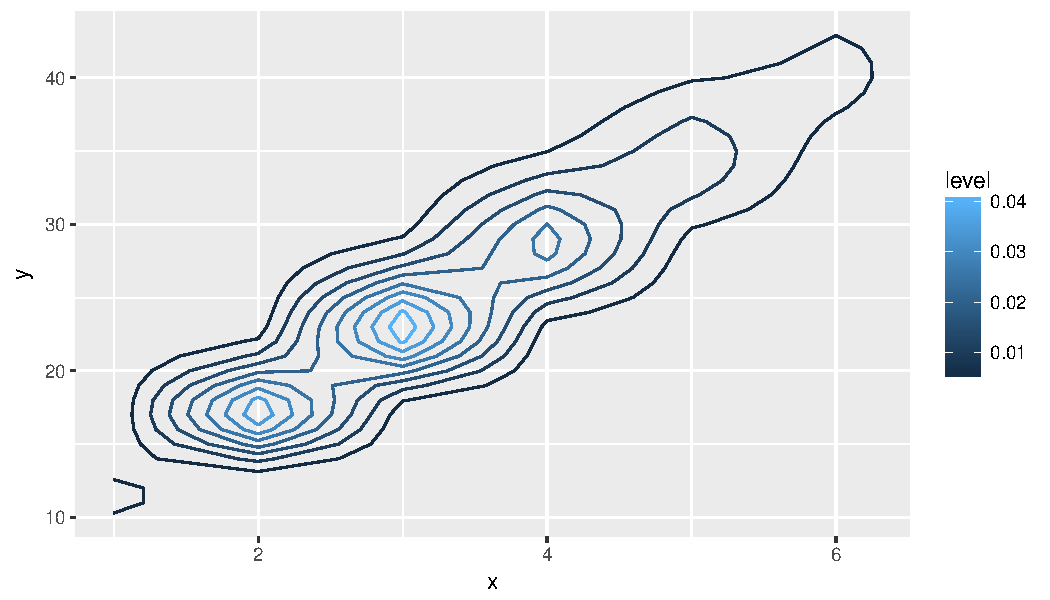
\includegraphics[width=\maxwidth]{figure/unnamed-chunk-70-1} 
\begin{kframe}\begin{alltt}
\hlcom{# gr\textbackslash{}'afica de perspectiva}
  \hlkwd{persp3D}\hlstd{(}\hlkwc{z}\hlstd{=mat,} \hlkwc{x}\hlstd{=a,} \hlkwc{y}\hlstd{=b)}
\end{alltt}
\end{kframe}
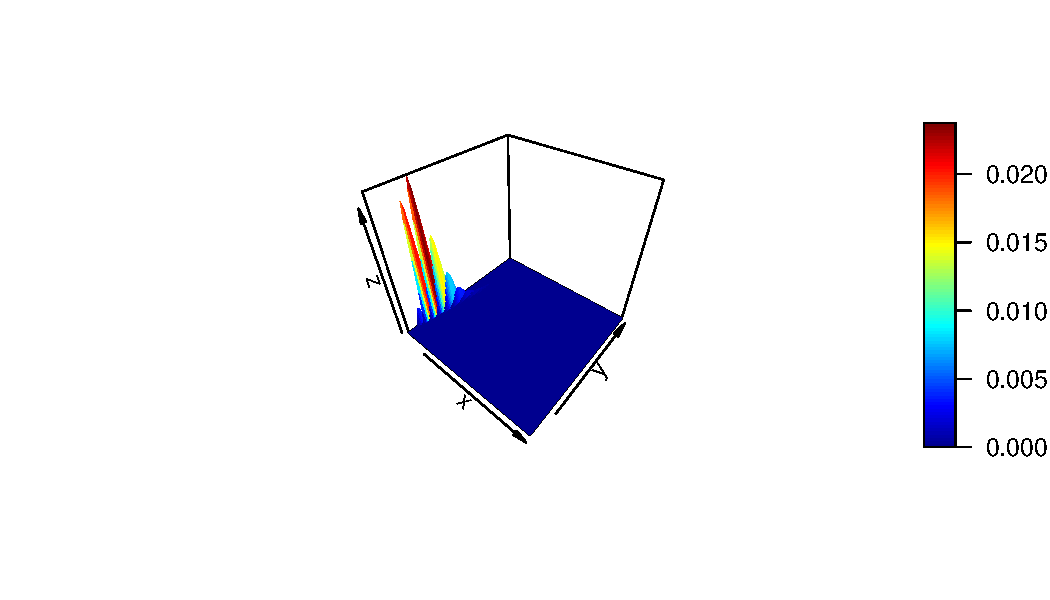
\includegraphics[width=\maxwidth]{figure/unnamed-chunk-70-2} 

\end{knitrout}

%\begin{figure}[!htb]
%\centering
%\includegraphics[scale=0.5]{congrilla.eps}
%\caption{\emph{Contorno de la distribuci\'on posterior de los hiperpar\'ametros $(\alpha, \beta)'$}}
%\end{figure}

%\begin{figure}[!htb]
%\centering
%\includegraphics[scale=0.5]{pergrilla.eps}
%\caption{\emph{Densidad bivariada de la distribuci\'on posterior de los hiperpar\'ametros $(\alpha, \beta)'$}}
%\end{figure}

\subsection{Modelo Poisson}
Ahora, suponga el modelo Poisson para los datos, dado por 
\begin{align*}
Y_i \mid \theta_i \sim Poisson(\theta_i)
\end{align*}

donde los $Y_i$ forman una sucesi\'on de variables aleatorias intercambiables y con cada par\'ametro $\theta_i$ ($i=1,\ldots,n$) distribuido como
\begin{align*}
\theta_i \mid (\alpha,\beta) \sim Gamma(\alpha,\beta)
\end{align*}

donde $\alpha$ y $\beta$ son hiperpar\'ametros desconocidos.Como estos hiperpar\'ametros son positivos ambos, es razonable asignarles la distribuci\'on $Gamma$ tales que
\begin{align*}
\alpha &\sim Gamma(a,b)\\
\beta &\sim Gamma(c,d)
\end{align*}

Usualmente los par\'ametros $a$, $b$, $c$ y $d$ son conocidos y son tales que las distribuciones de $\alpha$ y $\beta$ sean planas o no-informativas. De esta manera, el enfoque bayesiano jer\'arquico plantea que se debe realizar la inferencia conjunta para el vector de par\'ametros $\btheta=(\theta_1, \ldots, \theta_n)'$ y para $(\alpha, \beta)'$. Con base en lo anterior, la distribuci\'on posterior de los par\'ametros de inter\'es toma la siguiente forma
\begin{align*}
p(\btheta,\alpha,\beta \mid \mathbf{Y})&\propto
\prod_{i=1}^n p(Y\mid \theta_i)p(\theta_i\mid \alpha, \beta)p(\alpha)p(\beta)\\
&\propto \prod_{i=1}^n \frac{e^{-\theta_i}\theta_i^{y_i}}{y_i!}
\frac{\beta^\alpha}{\Gamma(\alpha)}\theta_i^{\alpha-1}e^{-\beta\theta_i}
e^{-\alpha b}\alpha^{a-1}e^{-\beta d}\beta^{c-1}
\end{align*}

Como es usual, y acudiendo a la anterior distribuci\'on posterior conjunta, se utilizar\'a la t\'ecnica del condicionamiento sucesivo para encontrar las distribuciones posterior marginales de cada uno de los par\'ametros de inter\'es. En este orden de ideas, se tiene que para cada $\theta_i$ con $i=1,\ldots,n$, la distribuci\'on posterior marginal est\'a dada por
\begin{align*}
p(\theta_i \mid \alpha,\beta,\theta_1,\ldots,\theta_{i-1},\theta_{i+1},\cdots,\theta_n,\mathbf{Y})
&\propto
p(\theta_i, \underbrace{\alpha,\beta,\theta_1,\ldots,\theta_{i-1},\theta_{i+1},\cdots,\theta_n}_{fijos}\mid\mathbf{Y})\\
&\propto e^{-\theta_i}\theta_i^{y_i}\theta_i^{\alpha-1}e^{-\beta\theta_i}\\
&= \exp\{-\theta_i(\beta+1)\}\theta^{y_i+\alpha-1}
\end{align*}

Con base en lo anterior, se tiene que la distribuci\'on posterior para cada par\'ametro $\theta_i$ es
\begin{equation*}
\theta_i\mid \alpha,\beta,\theta_1,\ldots,\theta_{i-1},\theta_{i+1},\theta_n,\mathbf{Y}
\sim Gamma(y_i+\alpha, \beta+1)
\end{equation*}

Para el hiperpar\'ametro $\alpha$, se tiene que la distribuci\'on posterior marginal est\'a dada por
\begin{align*}
p(\alpha\mid \beta, \btheta, \mathbf{Y})
&\propto p(\alpha, \underbrace{\beta,\btheta}_{fijos}\mid\mathbf{Y})\\
&\propto \prod_{i=1}^n \frac{\beta^\alpha\theta_i^{\alpha-1}}{\Gamma(\alpha)}\alpha^{a-1}\exp\{-\alpha b\}
\end{align*}

La anterior distribuci\'on no tiene una forma conocida y es necesario utilizar m\'etodos num\'ericos para simular observaciones de provenientes de \'esta. Para esto es posible utilizar el m\'etodo de la grilla.

Por \'ultimo, la distribuci\'on posterior marginal del hiperpar\'ametro $\beta$ se encuentra, similarmente mediante el condicionamiento sucesivo, de la siguiente forma
\begin{align*}
p(\beta \mid \alpha,\btheta,\mathbf{Y})
&\propto p(\beta, \underbrace{\alpha,\btheta}_{fijos}\mid\mathbf{Y})\\
&\propto \prod_{i=1}^n \beta^{\alpha}\exp\{-\beta\theta_i\}\beta^{c-1}\exp\{-\beta d\}\\
&=\beta^{n(\alpha+c-1)}\exp\left\{-\beta\left(nd+\sum_{i=1}^n\theta_i\right)\right\}
\end{align*}

Por lo tanto, se concluye que la distribuci\'on posterior para el hiperpar\'ametro $\beta$ es
\begin{equation*}
\beta\mid \alpha,\btheta,\mathbf{Y}
\sim Gamma\left(n(\alpha+c-1)+1, nd+\sum_{i=1}^n\theta_i\right)
\end{equation*}

Para realizar la inferencia bayesiana jer\'arquica para los par\'ametros de inter\'es se deben fijar valores iniciales para cada par\'ametro y mediante simulaci\'on renovarlos hasta obtener convergencia. Por ejemplo, un posible camino para obtener convergencia en la simulaci\'on se describe a continuaci\'on:

\begin{itemize}
  \item Fijar valores iniciales para $\alpha$ y $\beta$.
  \item Con los anteriores valores simular una observaci\'on para cada distribuci\'on posterior de los par\'ametros $\theta_i$ $(i=1,\ldots,n)$.
  \item Con estos valores de $\theta_i$ y el valor inicial de $\beta$, simular una observaci\'on de la distribuci\'on posterior de $\alpha$.
  \item Con los valores de $\theta_i$ y la anterior observaci\'on de $\alpha$, simular un nuevo valor para $\beta$.
  \item Repetir el anterior proceso hasta lograr convergencia.
\end{itemize}

Dado que las distribuciones posterior de los par\'ametros $\theta_i$ $(i=1,\ldots,n)$ y del hiperpar\'ametro $\beta$ est\'an ligadas a la distribuci\'on Gamma, la simulaci\'on para estos par\'ametros es f\'acil. Sin eambrgo, como la distribuci\'on posterior marginal de $\alpha$ no tiene una forma cerrada, es necesario implementar un c\'odigo propio en \verb'R' que permita simular un valor proveniente de esta distribuci\'on. Es posible utilizar el m\'etodo de la grilla que, en este caso, es univariado pues se trata de un s\'olo hiperpar\'ametro. Con base en lo anterior, se tiene la siguiente funci\'on que reproduce esta distribuci\'on no conocida.

\begin{knitrout}
\definecolor{shadecolor}{rgb}{0.933, 0.933, 0.933}\color{fgcolor}\begin{kframe}
\begin{alltt}
 \hlstd{post} \hlkwb{<-} \hlkwa{function}\hlstd{(}\hlkwc{theta}\hlstd{,} \hlkwc{alpha}\hlstd{,} \hlkwc{beta}\hlstd{,} \hlkwc{a}\hlstd{,} \hlkwc{b}\hlstd{)\{}
   \hlstd{P1} \hlkwb{<-} \hlstd{beta}\hlopt{^}\hlstd{alpha} \hlopt{*} \hlstd{(theta}\hlopt{^}\hlstd{(alpha}\hlopt{-}\hlnum{1}\hlstd{))} \hlopt{/} \hlkwd{gamma}\hlstd{(alpha)}
   \hlstd{P2} \hlkwb{<-} \hlstd{alpha}\hlopt{^}\hlstd{(a}\hlopt{-}\hlnum{1}\hlstd{)}
   \hlstd{P3} \hlkwb{<-}  \hlkwd{exp}\hlstd{(}\hlopt{-}\hlstd{alpha}\hlopt{*}\hlstd{beta)}
   \hlstd{res} \hlkwb{<-} \hlkwd{prod}\hlstd{(P1)}\hlopt{*}\hlstd{P2}\hlopt{*}\hlstd{P3}
   \hlstd{res}
 \hlstd{\}}
\end{alltt}
\end{kframe}
\end{knitrout}

Por ejemplo, suponga que $\btheta=(\theta_1, \theta_2, \theta_3)'$ cuyas observaciones, para una iteraci\'on en particular, fueron $(2, 2, 3)$ y que la observaci\'on para $\beta$ fue 0.9. De esta manera, se crea una grilla de los posibles valores que puede tomar $\alpha$ y mediante el  uso de la funci\'on \verb'sample' se simula un valor proveniente de esta distribuci\'on rara.

\begin{knitrout}
\definecolor{shadecolor}{rgb}{0.933, 0.933, 0.933}\color{fgcolor}\begin{kframe}
\begin{alltt}
 \hlcom{# creaci\textbackslash{}'on de la grilla para alpha}
 \hlstd{alpha.grid} \hlkwb{<-} \hlkwd{seq}\hlstd{(}\hlnum{0.05}\hlstd{,} \hlnum{20}\hlstd{,} \hlkwc{by}\hlstd{=}\hlnum{0.01}\hlstd{)}
 \hlstd{be} \hlkwb{<-} \hlnum{0.9}
 \hlstd{a1} \hlkwb{<-} \hlnum{2}
 \hlstd{b2} \hlkwb{<-} \hlnum{3}
 \hlstd{t} \hlkwb{<-} \hlkwd{c}\hlstd{(}\hlnum{2}\hlstd{,}\hlnum{2}\hlstd{,}\hlnum{3}\hlstd{)}

 \hlcom{# probabilidad para cada valor en la grilla}
 \hlstd{post.alpha} \hlkwb{<-} \hlkwd{c}\hlstd{()}
 \hlkwa{for}\hlstd{(k} \hlkwa{in} \hlnum{1}\hlopt{:}\hlkwd{length}\hlstd{(alpha.grid))\{}
  \hlstd{post.alpha[k]} \hlkwb{<-} \hlkwd{post}\hlstd{(t,alpha.grid[k],be,a1,b1)}
 \hlstd{\}}
 \hlstd{N.grid} \hlkwb{<-} \hlkwd{length}\hlstd{(post.alpha)}
 \hlstd{post.alpha} \hlkwb{<-} \hlstd{post.alpha}\hlopt{/}\hlkwd{sum}\hlstd{(post.alpha)}
 \hlkwd{sum}\hlstd{(post.alpha)}
\end{alltt}
\begin{verbatim}
## [1] 1
\end{verbatim}
\begin{alltt}
 \hlcom{# simulaci\textbackslash{}'on de una sola observaci\textbackslash{}'on}
 \hlstd{rpost} \hlkwb{<-} \hlkwd{sample}\hlstd{(N.grid,} \hlnum{1}\hlstd{,} \hlkwc{prob}\hlstd{=post.alpha,} \hlkwc{replace}\hlstd{=}\hlnum{TRUE}\hlstd{)}
 \hlstd{r.alpha} \hlkwb{<-} \hlstd{alpha.grid[rpost]}
 \hlstd{r.alpha}
\end{alltt}
\begin{verbatim}
## [1] 3.7
\end{verbatim}
\end{kframe}
\end{knitrout}

Por otro lado, en t\'erminos exploratorios, es posible simular varios valores de la distribuci\'on no conocida y determinar qu\'e forma tiene. Para la anterior configuraci\'on, y utilizando el siguiente c\'odigo, se simularon 100 valores de esta distribuci\'on. En general, es posible afirmar que su forma es parecida a la de una distribuci\'on gamma, esto tiene sentido pues est\'a en funci\'on de distribuciones gamma, sesgadas a la derecha y unimodales.

\begin{knitrout}
\definecolor{shadecolor}{rgb}{0.933, 0.933, 0.933}\color{fgcolor}\begin{kframe}
\begin{alltt}
\hlcom{# corroborar la estructura de la cadena}
\hlstd{N.sim} \hlkwb{<-} \hlnum{1000}

\hlstd{rpost} \hlkwb{<-} \hlkwd{sample}\hlstd{(N.grid, N.sim,} \hlkwc{prob}\hlstd{=post.alpha,} \hlkwc{replace}\hlstd{=}\hlnum{TRUE}\hlstd{)}
\hlstd{r.alpha} \hlkwb{<-} \hlstd{alpha.grid[rpost]}
\hlkwd{mean}\hlstd{(r.alpha)}
\end{alltt}
\begin{verbatim}
## [1] 2.4
\end{verbatim}
\begin{alltt}
\hlkwd{plot}\hlstd{(r.alpha)}
\end{alltt}
\end{kframe}
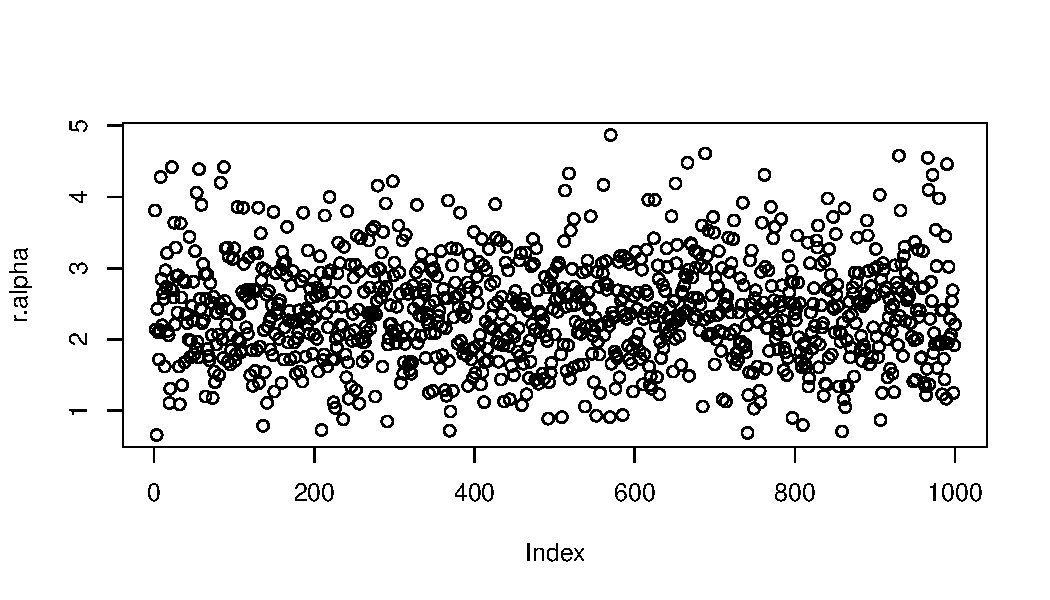
\includegraphics[width=\maxwidth]{figure/unnamed-chunk-73-1} 
\begin{kframe}\begin{alltt}
\hlkwd{hist}\hlstd{(r.alpha,} \hlkwc{breaks}\hlstd{=}\hlnum{20}\hlstd{)}
\end{alltt}
\end{kframe}
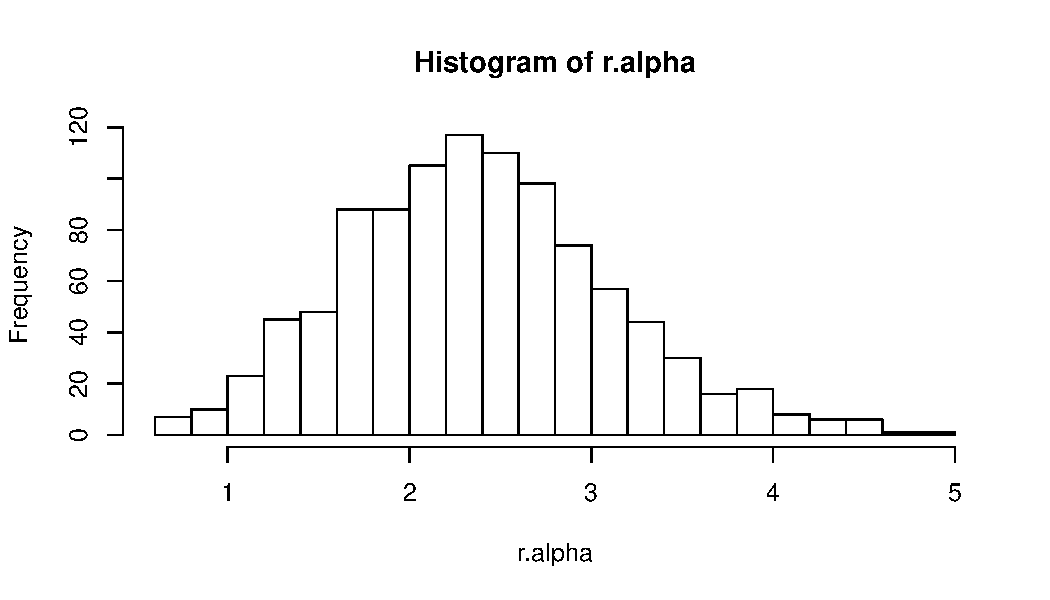
\includegraphics[width=\maxwidth]{figure/unnamed-chunk-73-2} 
\begin{kframe}\begin{alltt}
\hlkwd{ts.plot}\hlstd{(post.alpha)}
\end{alltt}
\end{kframe}
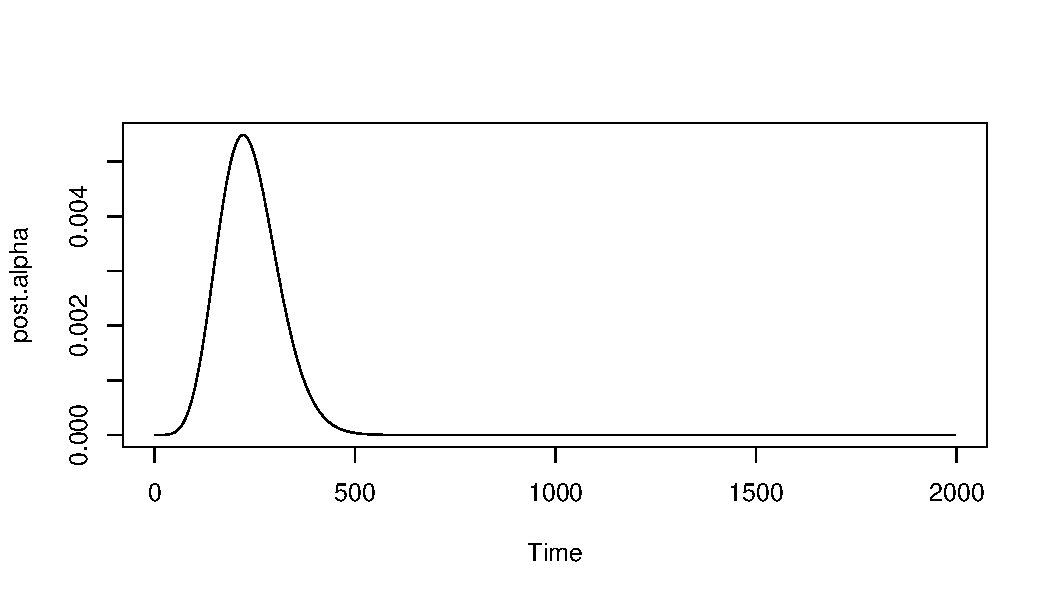
\includegraphics[width=\maxwidth]{figure/unnamed-chunk-73-3} 

\end{knitrout}
Ahora ilustramos el procedimiento de obtener la estimaci\'on de $\alpha$, $\beta$ y los $\theta_i$ usando suponiendo que se quiere estimar el n\'umero de accidentes de tr\'ansito relacionados con motociclistas en las veinte localidades de la ciudad de Bogot\'a, suponga que en un mismo d\'ia determinado los n\'umeros de estos accidentes son: $6, 5, 9, 2, 3, 0, 4, 1, 1, 2, 1, 6, 7, 2, 4, 3, 0, 4, 3, 2$.
\begin{knitrout}
\definecolor{shadecolor}{rgb}{0.933, 0.933, 0.933}\color{fgcolor}\begin{kframe}
\begin{alltt}
\hlstd{y} \hlkwb{<-} \hlkwd{c}\hlstd{(}\hlnum{6}\hlstd{,} \hlnum{5}\hlstd{,} \hlnum{9}\hlstd{,} \hlnum{2}\hlstd{,} \hlnum{3}\hlstd{,} \hlnum{0}\hlstd{,} \hlnum{4}\hlstd{,} \hlnum{1}\hlstd{,} \hlnum{1}\hlstd{,} \hlnum{2}\hlstd{,} \hlnum{1}\hlstd{,} \hlnum{6}\hlstd{,} \hlnum{7}\hlstd{,} \hlnum{2}\hlstd{,} \hlnum{4}\hlstd{,} \hlnum{3}\hlstd{,} \hlnum{0}\hlstd{,} \hlnum{4}\hlstd{,} \hlnum{3}\hlstd{,} \hlnum{2}\hlstd{)}
\hlstd{n} \hlkwb{<-} \hlkwd{length}\hlstd{(y)}
\hlstd{n.sim} \hlkwb{<-} \hlnum{1000}
\hlstd{res.theta} \hlkwb{<-} \hlkwd{matrix}\hlstd{(}\hlnum{NA}\hlstd{,n.sim,n); res.beta} \hlkwb{<-} \hlkwd{c}\hlstd{(); res.alpha} \hlkwb{<-} \hlkwd{c}\hlstd{()}
\hlcom{# Valor inicial para theta}
\hlstd{res.theta[}\hlnum{1}\hlstd{,]} \hlkwb{<-} \hlnum{20}
\hlcom{# Valor inicial para beta}
\hlstd{res.beta[}\hlnum{1}\hlstd{]} \hlkwb{<-} \hlnum{1}
\hlcom{# Simular un valor para alpha}
 \hlcom{# creaci\textbackslash{}'on de la grilla para alpha}
 \hlstd{alpha.grid} \hlkwb{<-} \hlkwd{seq}\hlstd{(}\hlnum{0.05}\hlstd{,} \hlnum{20}\hlstd{,} \hlkwc{by}\hlstd{=}\hlnum{0.01}\hlstd{)}
 \hlstd{a} \hlkwb{<-} \hlstd{c} \hlkwb{<-} \hlnum{2}
 \hlstd{b} \hlkwb{<-} \hlstd{d} \hlkwb{<-} \hlnum{3}
 \hlcom{# probabilidad para cada valor en la grilla}
 \hlstd{post.alpha} \hlkwb{<-} \hlkwd{c}\hlstd{()}
 \hlkwa{for}\hlstd{(k} \hlkwa{in} \hlnum{1}\hlopt{:}\hlkwd{length}\hlstd{(alpha.grid))\{}
  \hlstd{post.alpha[k]} \hlkwb{<-} \hlkwd{post}\hlstd{(res.theta[}\hlnum{1}\hlstd{,], alpha.grid[k], res.beta[}\hlnum{1}\hlstd{],a,b)}
 \hlstd{\}}
 \hlstd{N.grid} \hlkwb{<-} \hlkwd{length}\hlstd{(post.alpha)}
 \hlstd{post.alpha} \hlkwb{<-} \hlstd{post.alpha}\hlopt{/}\hlkwd{sum}\hlstd{(post.alpha)}
 \hlstd{res.alpha[}\hlnum{1}\hlstd{]} \hlkwb{<-} \hlstd{alpha.grid[}\hlkwd{sample}\hlstd{(}\hlkwd{length}\hlstd{(alpha.grid),} \hlnum{1}\hlstd{,} \hlkwc{prob}\hlstd{=post.alpha,} \hlkwc{replace}\hlstd{=}\hlnum{TRUE}\hlstd{)]}
 \hlcom{# Aqu?? comienza a simular los valores de los par\textbackslash{}'ametros}
 \hlkwa{for}\hlstd{(i} \hlkwa{in} \hlnum{2}\hlopt{:}\hlstd{n.sim)\{}
 \hlcom{# Simular un valor para theta}
   \hlkwa{for}\hlstd{(j} \hlkwa{in} \hlnum{1}\hlopt{:}\hlstd{n)\{}
     \hlstd{res.theta[i,j]} \hlkwb{<-} \hlkwd{rgamma}\hlstd{(}\hlnum{1}\hlstd{,} \hlkwc{shape}\hlstd{=y[j]}\hlopt{+}\hlstd{res.alpha[i}\hlopt{-}\hlnum{1}\hlstd{],} \hlkwc{rate}\hlstd{=res.beta[i}\hlopt{-}\hlnum{1}\hlstd{]}\hlopt{+}\hlnum{1}\hlstd{)}
   \hlstd{\}}
 \hlcom{# Simular un valor para beta}
   \hlstd{res.beta[i]} \hlkwb{<-} \hlkwd{rgamma}\hlstd{(}\hlnum{1}\hlstd{, n}\hlopt{*}\hlstd{(res.alpha[i}\hlopt{-}\hlnum{1}\hlstd{]}\hlopt{+}\hlstd{c}\hlopt{-}\hlnum{1}\hlstd{)}\hlopt{+}\hlnum{1}\hlstd{,} \hlkwc{rate}\hlstd{=n}\hlopt{*}\hlstd{d}\hlopt{+}\hlkwd{sum}\hlstd{(res.theta[i,]))}
 \hlcom{# Simular un valor para alpha}
 \hlstd{post.alpha} \hlkwb{<-} \hlkwd{c}\hlstd{()}
 \hlkwa{for}\hlstd{(k} \hlkwa{in} \hlnum{1}\hlopt{:}\hlkwd{length}\hlstd{(alpha.grid))\{}
  \hlstd{post.alpha[k]} \hlkwb{<-} \hlkwd{post}\hlstd{(res.theta[i,],alpha.grid[k],res.beta[i],a,b)}
 \hlstd{\}}
 \hlstd{post.alpha} \hlkwb{<-} \hlstd{post.alpha}\hlopt{/}\hlkwd{sum}\hlstd{(post.alpha)}

 \hlstd{res.alpha[i]} \hlkwb{<-} \hlstd{alpha.grid[}\hlkwd{sample}\hlstd{(}\hlkwd{length}\hlstd{(post.alpha),} \hlnum{1}\hlstd{,} \hlkwc{prob}\hlstd{=post.alpha,} \hlkwc{replace}\hlstd{=}\hlnum{TRUE}\hlstd{)]}
 \hlstd{\}}
 \hlcom{# Verificar la convergencia de algunos par??metros}
 \hlkwd{par}\hlstd{(}\hlkwc{mfrow}\hlstd{=}\hlkwd{c}\hlstd{(}\hlnum{2}\hlstd{,}\hlnum{2}\hlstd{))}
 \hlkwd{ts.plot}\hlstd{(res.theta[,}\hlnum{1}\hlstd{]);} \hlkwd{ts.plot}\hlstd{(res.theta[,}\hlnum{2}\hlstd{])}
 \hlkwd{ts.plot}\hlstd{(res.alpha);} \hlkwd{ts.plot}\hlstd{(res.beta)}
\end{alltt}
\end{kframe}
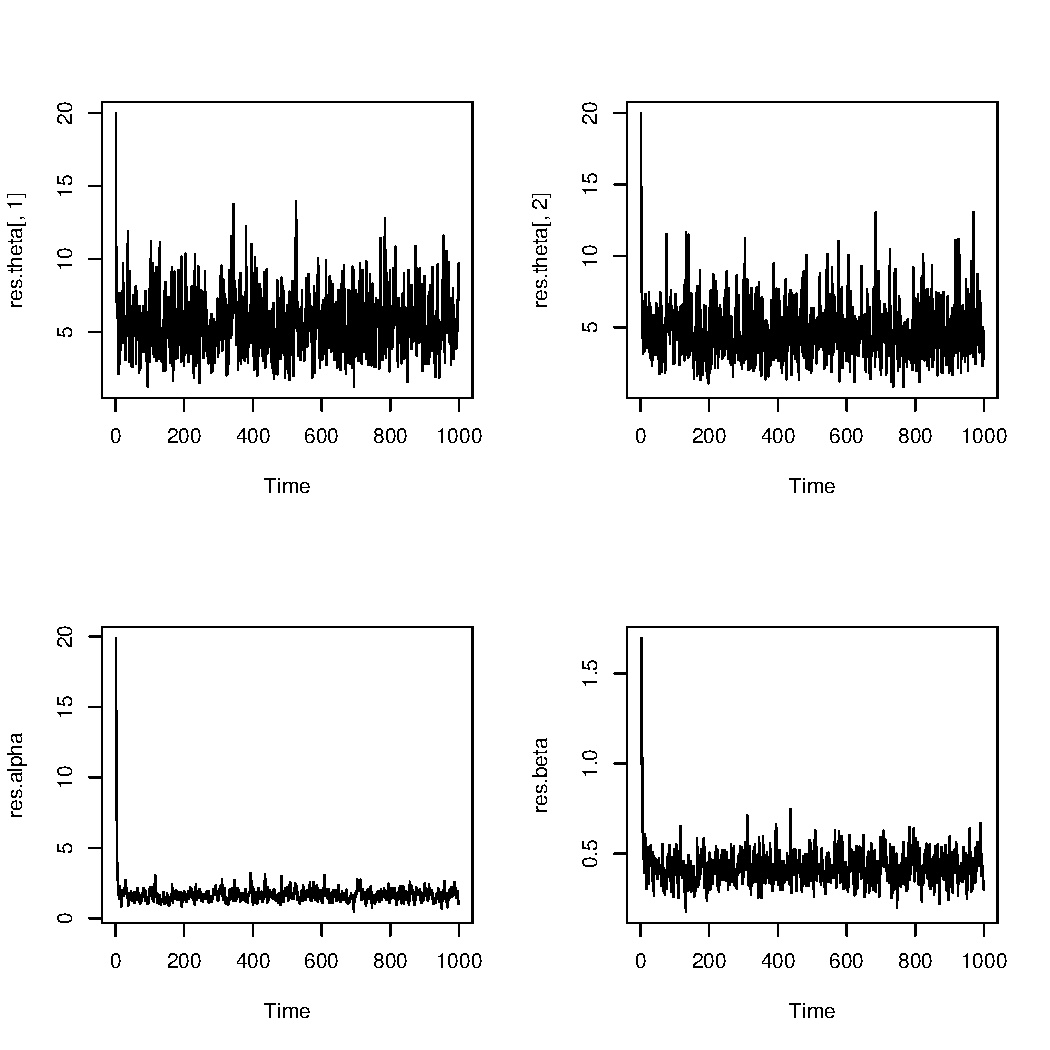
\includegraphics[width=\maxwidth]{figure/unnamed-chunk-74-1} 
\begin{kframe}\begin{alltt}
 \hlcom{# Calcular la estimaci\textbackslash{}'on de los par\textbackslash{}'ametros tomando la segunda mitad de los valores simulados}
 \hlkwd{colMeans}\hlstd{(res.theta[}\hlopt{-}\hlstd{(}\hlnum{1}\hlopt{:}\hlstd{(n.sim}\hlopt{/}\hlnum{2}\hlstd{)),])}
\end{alltt}
\begin{verbatim}
##  [1] 5.6 4.7 7.5 2.6 3.3 1.1 3.9 1.9 1.9 2.5 1.8 5.4 6.0 2.6 3.9 3.4 1.2
## [18] 3.8 3.2 2.6
\end{verbatim}
\begin{alltt}
 \hlkwd{mean}\hlstd{(res.alpha[}\hlopt{-}\hlstd{(}\hlnum{1}\hlopt{:}\hlstd{(n.sim}\hlopt{/}\hlnum{2}\hlstd{))])}
\end{alltt}
\begin{verbatim}
## [1] 1.7
\end{verbatim}
\begin{alltt}
 \hlkwd{mean}\hlstd{(res.beta[}\hlopt{-}\hlstd{(}\hlnum{1}\hlopt{:}\hlstd{(n.sim}\hlopt{/}\hlnum{2}\hlstd{))])}
\end{alltt}
\begin{verbatim}
## [1] 0.42
\end{verbatim}
\end{kframe}
\end{knitrout}

El anterior desarrollo te\'orico tambi\'en se puede adaptar para el caso cuando se asume la misma media para todas las variables observadas, esto es, $Y_i\mid\theta$ para $i=1,\cdots,n$. En este caso, se tiene que 
\begin{equation*}
p(\theta,\alpha,\beta\mid\mathbf{Y})\propto e^{-(n+\beta)\theta}\theta^{\sum y_i+\alpha-1}\beta^{\alpha+c-1}e^{-\alpha b-\beta d}\alpha^{a-1}/\Gamma(\alpha)
\end{equation*}

de donde se puede concluir que 
\begin{align}
\theta\mid\alpha,\beta,\mathbf{Y}&\sim Gamma(\sum y_i+\alpha,n+\beta)\label{Poisson_Gamma1}\\
\alpha\mid\theta,\beta,\mathbf{Y}&\propto(\theta\beta)^\alpha e^{-\alpha b}\alpha^{a-1}/\Gamma(\alpha)\label{Poisson_Gamma2}\\
\beta\mid\theta,\alpha,\mathbf{Y}&\sim Gamma(\alpha+c,\theta+d)\label{Poisson_Gamma3}
\end{align}

\subsection{Modelo Normal}
Considere una variaci\'on de la estructura jer\'arquica de la secci\'on \ref{Normal_Normal}, en donde las observaciones siguen el siguiente modelo de probabilidad
\begin{equation*}
Y_i \mid \theta_i \sim Normal(\theta_i,\sigma^2) \ \ \ \ \ \ \ i=1,\ldots,n
\end{equation*}

y el par\'ametro $\sigma^2$ se supone conocido. Sin embargo, la distribuci\'on previa para los par\'ametros de inter\'es $\theta_i$ es
\begin{equation*}
\theta_i \mid \mu \sim Normal(\mu, \tau^2) \ \ \ \ \ \ \ i=1,\ldots,n
\end{equation*}
en donde los par\'ametros $\mu$ y $\tau^2$ son desconocidos. De esta forma, es necesario hallar una forma de estimar los valores de estos dos hiperpar\'ametros, esto se puede llevar a cabo considerando diferente estructuras de dependencia entre $mu$ y $\tau^2$. 

\subsubsection{Hiperpar\'ametros independientes}
En primer lugar, supongamos que los hiperpar\'ametros son independientes en la distribuci\'on previa, es decir que su funci\'on de densidad conjunta se puede factorizar como el producto de las distribuciones marginales de cada uno de los hiperpar\'ametros. m\'as a\'un, si se supone que las distribuciones previa marginales son no informativas y siguen una estructura probabil\'istica uniforme, entonces se tiene que
\begin{equation*}
p(\mu,\tau^2)=p(\mu)p(\tau^2)\propto k
\end{equation*}

Con esta formulaci\'on se deduce que la distribuci\'on posterior conjunta condicional a una sola observaci\'on est\'a dada por
\begin{align}
p(\theta_i,\mu,\tau^2 \mid Y_i) &\propto p(Y_i \mid \theta_i)p(\theta_i \mid \mu,\tau^2)p(\mu,\tau^2) \notag \\
&\propto p(Y_i \mid \theta_i)p(\theta_i \mid \mu,\tau^2) \notag \\
&\propto \exp\left\{-\frac{1}{2\sigma^2}(y_i-\theta_i)^2\right\}
\frac{1}{\tau}\exp\left\{-\frac{1}{2\tau^2}(\theta_i-\mu)^2\right\}
\end{align}

Y la distribuci\'on distribuci\'on posterior conjunta condicional a todas las observaciones y a todos los par\'ametros de inter\'es es
\begin{align*}
p(\btheta,\mu,\tau^2 \mid \mathbf{Y})
&\propto p(\mathbf{Y} \mid \btheta)p(\btheta \mid \mu,\tau^2)  \\
&\propto \prod_{i=1}^n p(Y_i \mid \theta_i) \prod_{i=1}^n p(\theta_i \mid \mu,\tau^2)  \\
&\propto \exp\left\{\frac{1}{2\sigma^2}\sum_{i=1}^n(y_i-\theta_i)^2\right\}
\frac{1}{\tau^n}\exp\left\{\frac{1}{2\tau^2}\sum_{i=1}^n(\theta_i-\mu)^2\right\}
\end{align*}

Utilizaremos la t\'ecnica del condicionamiento para encontrar la distribuci\'on condicional del vector de par\'ametros de inter\'es $\btheta$ y de los hiperpar\'ametros. Por lo tanto se tiene que
\begin{align*}
p(\btheta \mid \mu,\tau^2,\mathbf{Y})
&\propto p(\btheta,\underbrace{\mu,\tau^2}_{fijos},\mathbf{Y})\\
p(\mu \mid \btheta,\tau^2,\mathbf{Y})
&\propto p(\mu,\underbrace{\btheta,\tau^2}_{fijos},\mathbf{Y}) \\
p(\tau^2 \mid \btheta,\mu,\mathbf{Y})
&\propto p(\mu,\underbrace{\btheta,\tau^2}_{fijos},\mathbf{Y})
\end{align*}

Con la anterior formulaci\'on se tiene la siguiente serie de resultados que dan cuenta de las distribuciones apropiadas para cada uno de los par\'ametros.

\begin{Res}
La distribuci\'on posterior del par\'ametro de inter\'es $\theta_i$ es
\begin{equation*}
\theta_i\sim Normal(\mu_i,\tau_1^2)
\end{equation*}
en donde
\begin{equation*}
\mu_i=\frac{\frac{1}{\sigma^2}Y_i+\frac{1}{\tau^2}\mu}{\frac{1}{\sigma^2}+\frac{1}{\tau^2}}
\ \ \ \ \ \ \ \text{y} \ \ \ \ \ \ \
\tau_1^2=\left(\frac{1}{\sigma^2}+\frac{1}{\tau^2}\right)^{-1}
\end{equation*}
\end{Res}

\begin{proof}
Utilizando la t\'ecnica del condicionamiento posterior se tiene que
\begin{align*}
p(\theta_i \mid \mu,\tau^2,Y_i)
&\propto p(\theta_i,\underbrace{\mu,\tau^2}_{fijos},Y_i)\\
&\propto \exp\left\{-\frac{1}{2\sigma^2}(y_i-\theta_i)^2-\frac{1}{2\tau^2}(\theta_i-\mu)^2\right\}
\end{align*}
y utilizando el mismo razonamiento que en la demostraci\'on del Resultado 2.6.1 se encuentra una expresi\'on id\'entica a la funci\'on de distribuci\'on de una variable aleatoria con distribuci\'on $Normal(\mu_i,\tau_1^2)$.
\end{proof}

\begin{Res}
La distribuci\'on posterior del hiper-par\'ametro $\mu$ es
\begin{equation*}
\mu\sim Normal(\bar{\theta},\tau^2/n)
\end{equation*}
en donde $\bar{\theta}=\dfrac{1}{n}\sum_{i=1}^n\theta_i$.
\end{Res}

\begin{proof}
Utilizando la t\'ecnica del condicionamiento posterior y teniendo en cuenta que
\begin{equation*}
\sum_{i=1}^n(\theta_i-\mu)^2=\sum_{i=1}^n(\theta_i-\bar{\theta})^2+n(\mu-\bar{\theta})^2
\end{equation*}

entonces, se tiene que
\begin{align*}
p(\mu \mid \btheta,\tau^2,\mathbf{Y})
&\propto p(\mu,\underbrace{\btheta,\tau^2}_{fijos},\mathbf{Y})\\
&\propto \exp\left\{-\frac{1}{2\tau^2}\sum_{i=1}^n(\theta_i-\mu)^2\right\}
 \propto \exp\left\{-\frac{n}{2\tau^2}(\mu-\bar{\theta})^2\right\}
\end{align*}
Por lo tanto, factorizando convenientemente, se encuentra una expresi\'on id\'entica a la funci\'on de distribuci\'on de una variable aleatoria con distribuci\'on $Normal(\bar{\theta},\tau^2/n)$.
\end{proof}

\begin{Res}
La distribuci\'on posterior del hiper-par\'ametro $\tau^2$ es
\begin{equation*}
\tau^2 \sim Inversa-Gamma(n/2-1,nS^2_{\mu}/2)
\end{equation*}
en donde $nS^2_{\mu}=\sum_{i=1}^n(\theta_i-\mu)^2$.
\end{Res}

\begin{proof}
Utilizando la t\'ecnica del condicionamiento posterior se tiene que
\begin{align*}
p(\tau^2 \mid \btheta,\mu,\mathbf{Y})
&\propto p(\tau^2,\underbrace{\btheta,\mu}_{fijos},\mathbf{Y})\\
&\propto \frac{1}{\tau^n} \exp\left\{\frac{1}{2\tau^2}\sum_{i=1}^n(\theta_i-\mu)^2\right\}\\
&\propto \left(\tau^2\right)^{-n/2} \exp\left\{\frac{nS^2_{\mu}}{2\tau^2}\right\}
\end{align*}
Por lo tanto, factorizando convenientemente, se encuentra una expresi\'on id\'entica a la funci\'on de distribuci\'on de una variable aleatoria con distribuci\'on $Inversa-Gamma(n/2-1,nS^2_{\mu}/2)$.
\end{proof}

Utilizando un algoritmo que genere una cadena de Markov, y utilizando los anteriores resultados se realiza un an\'alisis bayesiano propiamente dicho.

Ilustramos la implementaci\'on en \verb'R' a continuaci\'on para datos de $y$ de 5.8, 4.7, 7.0, 8.3, 3.7, 3.7, 5.5, 7.7, 6.7 y 6.7, usando $\sigma^2=1$.
\begin{knitrout}
\definecolor{shadecolor}{rgb}{0.933, 0.933, 0.933}\color{fgcolor}\begin{kframe}
\begin{alltt}
\hlkwd{library}\hlstd{(pscl)}
\hlstd{y} \hlkwb{<-} \hlkwd{c}\hlstd{(}\hlnum{5.8}\hlstd{,} \hlnum{4.7}\hlstd{,} \hlnum{7.0}\hlstd{,} \hlnum{8.3}\hlstd{,} \hlnum{3.7}\hlstd{,} \hlnum{3.7}\hlstd{,} \hlnum{5.5}\hlstd{,} \hlnum{7.7}\hlstd{,} \hlnum{6.7}\hlstd{,} \hlnum{6.7}\hlstd{)}
\hlstd{n} \hlkwb{<-} \hlkwd{length}\hlstd{(y); sigma2} \hlkwb{<-} \hlnum{1}
\hlstd{n.sim} \hlkwb{<-} \hlnum{1000}
\hlcom{# Espacio para guardar los resultados simulados}
\hlstd{res.mu} \hlkwb{<-} \hlkwd{rep}\hlstd{(}\hlnum{0}\hlstd{, n.sim); res.tau2} \hlkwb{<-} \hlkwd{rep}\hlstd{(}\hlnum{1}\hlstd{, n.sim); res.theta}\hlkwb{<-} \hlkwd{matrix}\hlstd{(}\hlnum{NA}\hlstd{, n.sim, n)}
\hlcom{# Simular el primer valor para theta}
\hlstd{tau2_1} \hlkwb{<-} \hlstd{(sigma2}\hlopt{^-}\hlnum{1} \hlopt{+} \hlstd{res.tau2[}\hlnum{1}\hlstd{]}\hlopt{^-}\hlnum{1}\hlstd{)}\hlopt{^-}\hlnum{1}
\hlstd{mu_i} \hlkwb{<-} \hlstd{(y}\hlopt{/}\hlstd{sigma2} \hlopt{+} \hlstd{res.mu[}\hlnum{1}\hlstd{]}\hlopt{/}\hlstd{res.tau2[}\hlnum{1}\hlstd{])}\hlopt{*}\hlstd{tau2_1}
\hlkwa{for}\hlstd{(j} \hlkwa{in} \hlnum{1}\hlopt{:}\hlstd{n)\{}
  \hlstd{res.theta[}\hlnum{1}\hlstd{,j]} \hlkwb{<-} \hlkwd{rnorm}\hlstd{(}\hlnum{1}\hlstd{, mu_i[j],} \hlkwd{sqrt}\hlstd{(tau2_1))}
\hlstd{\}}
\hlcom{# Aqu?? comienza a simular valores para todos los par\textbackslash{}'ametros}
\hlkwa{for}\hlstd{(i} \hlkwa{in} \hlnum{2}\hlopt{:}\hlstd{n.sim)\{}
  \hlstd{res.mu[i]} \hlkwb{<-} \hlkwd{rnorm}\hlstd{(}\hlnum{1}\hlstd{,} \hlkwd{mean}\hlstd{(res.theta[i}\hlopt{-}\hlnum{1}\hlstd{,]),} \hlkwd{sqrt}\hlstd{(res.tau2[i}\hlopt{-}\hlnum{1}\hlstd{]}\hlopt{/}\hlstd{n))}
  \hlstd{res.tau2[i]} \hlkwb{<-} \hlkwd{rigamma}\hlstd{(}\hlnum{1}\hlstd{,} \hlkwc{alpha}\hlstd{=n}\hlopt{/}\hlnum{2}\hlopt{-}\hlnum{1}\hlstd{,} \hlkwc{beta}\hlstd{=}\hlkwd{sum}\hlstd{((res.theta[i}\hlopt{-}\hlnum{1}\hlstd{,]}\hlopt{-}\hlstd{res.mu[i])}\hlopt{^}\hlnum{2}\hlstd{)}\hlopt{/}\hlnum{2}\hlstd{)}
  \hlstd{tau2_1} \hlkwb{<-} \hlstd{(sigma2}\hlopt{^-}\hlnum{1} \hlopt{+} \hlstd{res.tau2[i]}\hlopt{^-}\hlnum{1}\hlstd{)}\hlopt{^-}\hlnum{1}
  \hlstd{mu_i} \hlkwb{<-} \hlstd{(y}\hlopt{/}\hlstd{sigma2} \hlopt{+} \hlstd{res.mu[i]}\hlopt{/}\hlstd{res.tau2[i])}\hlopt{*}\hlstd{tau2_1}
  \hlkwa{for}\hlstd{(j} \hlkwa{in} \hlnum{1}\hlopt{:}\hlstd{n)\{}
    \hlstd{res.theta[i,j]} \hlkwb{<-} \hlkwd{rnorm}\hlstd{(}\hlnum{1}\hlstd{, mu_i[j],} \hlkwd{sqrt}\hlstd{(tau2_1))}
  \hlstd{\}}
\hlstd{\}}
 \hlcom{# Verificar la convergencia de algunos par??metros}
 \hlkwd{par}\hlstd{(}\hlkwc{mfrow}\hlstd{=}\hlkwd{c}\hlstd{(}\hlnum{2}\hlstd{,}\hlnum{2}\hlstd{))}
 \hlkwd{ts.plot}\hlstd{(res.theta[,}\hlnum{1}\hlstd{]);} \hlkwd{ts.plot}\hlstd{(res.theta[,}\hlnum{2}\hlstd{])}
 \hlkwd{ts.plot}\hlstd{(res.mu);} \hlkwd{ts.plot}\hlstd{(res.tau2)}
\end{alltt}
\end{kframe}
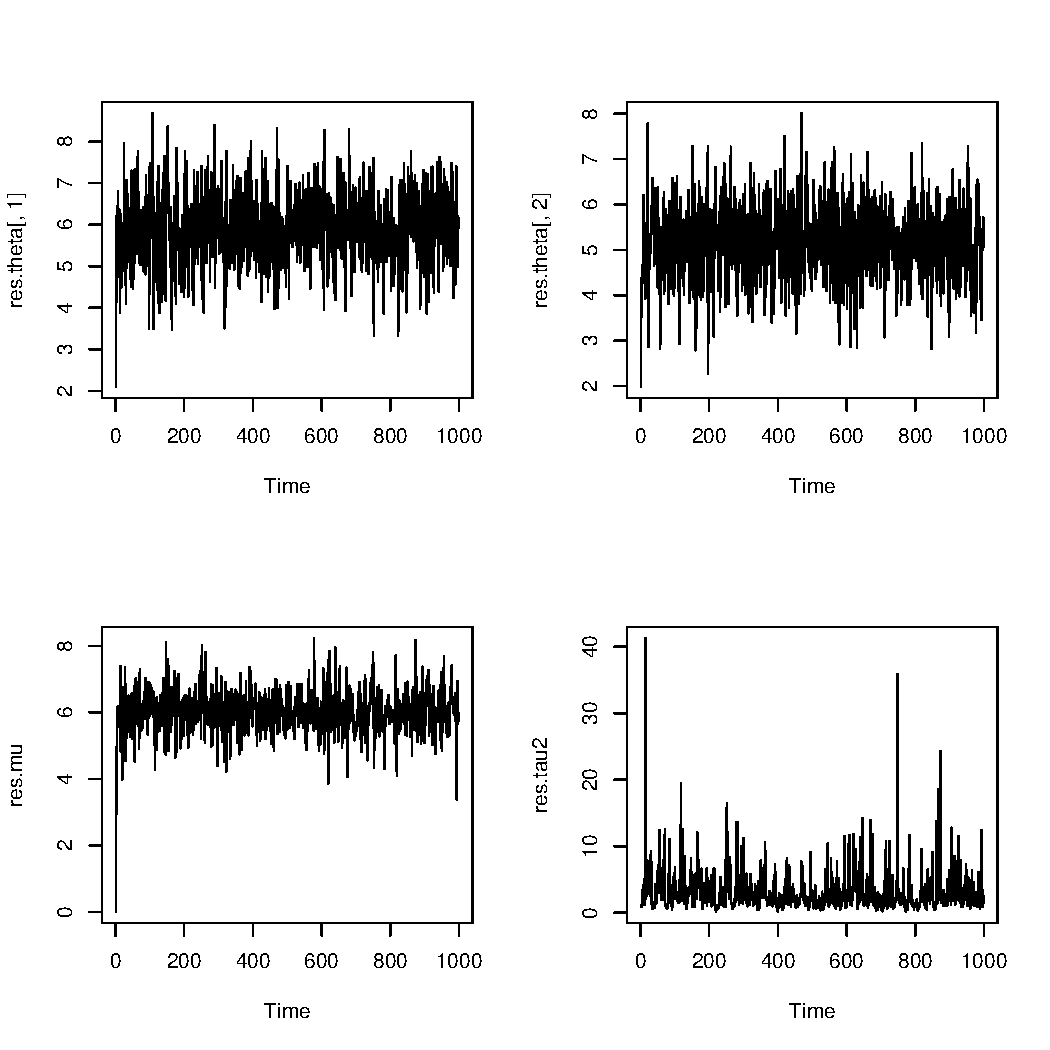
\includegraphics[width=\maxwidth]{figure/unnamed-chunk-75-1} 
\begin{kframe}\begin{alltt}
 \hlcom{# Calcular la estimaci\textbackslash{}'on de los par\textbackslash{}'ametros tomando la segunda mitad de los valores simulados}
 \hlkwd{colMeans}\hlstd{(res.theta[}\hlopt{-}\hlstd{(}\hlnum{1}\hlopt{:}\hlstd{(n.sim}\hlopt{/}\hlnum{2}\hlstd{)),])}
\end{alltt}
\begin{verbatim}
##  [1] 6.0 5.1 6.6 7.5 4.4 4.5 5.7 7.1 6.5 6.5
\end{verbatim}
\begin{alltt}
 \hlkwd{mean}\hlstd{(res.mu[}\hlopt{-}\hlstd{(}\hlnum{1}\hlopt{:}\hlstd{(n.sim}\hlopt{/}\hlnum{2}\hlstd{))])}
\end{alltt}
\begin{verbatim}
## [1] 6
\end{verbatim}
\begin{alltt}
 \hlkwd{mean}\hlstd{(res.tau2[}\hlopt{-}\hlstd{(}\hlnum{1}\hlopt{:}\hlstd{(n.sim}\hlopt{/}\hlnum{2}\hlstd{))])}
\end{alltt}
\begin{verbatim}
## [1] 3.1
\end{verbatim}
\end{kframe}
\end{knitrout}

Ahora consideramos el caso cuando la media de las variables observadas es com\'un, esto es, $Y_i\mid\theta\sim Normal(\theta,\sigma^2)$ y $\theta\mid\mu\sim Normal(\mu,\tau^2)$ para $i=1,\cdots,n$, asumimos la misma distribuci\'on no informativa para $\mu$ y $\tau^2$. En este caso tenemos que
\begin{equation*}
p(\theta,\mu,\tau^2\mid\mathbf{Y})\propto\exp\left\{-\frac{1}{2\sigma^2}\sum_i(y_i-\theta)^2\right\}
\frac{1}{\tau}\exp\left\{-\frac{1}{2\tau^2}(\theta-\mu)^2\right\}
\end{equation*}

De la expresi\'on se tiene que 
\begin{align}
\theta\mid\mu,\tau^2,\mathbf{Y}&\sim Normal(\mu_n,\tau^2_n)\label{Normal_N_1}\\
\mu\mid\theta,\tau^2,\mathbf{Y}&\sim Normal(\theta,\tau^2)\label{Normal_N_2}\\
p(\tau^2\mid\theta,\mu,\mathbf{Y})&\propto (\tau^2)^{-1/2}\exp\left\{-\frac{(\theta-\mu)^2}{2\tau^2}\right\}\label{Normal_N_3}
\end{align}

con $\tau^2_n=(\frac{n}{\sigma^2}+\frac{1}{\tau^2})^{-1}$ y $\mu_n=\tau^2_n(\frac{n\bar{y}}{\sigma^2}+\frac{\mu}{\tau^2})$. La expresi\'on en (\ref{Normal_N_3}) no corresponde a ninguna distribuci\'on con forma conocida, y debe hacer uso de m\'etodos de simulaci\'on para muestrear valores de $\tau^2$


\subsubsection{Hiperpar\'ametros dependientes}
Siguiendo el algoritmo dado al comienzo de esta secci\'on, en donde se dan los lineamentos generales para realizar un an\'alisis jer\'arquico. En primer lugar se debe considerar la distribuci\'on posterior de los par\'ametros, que en este caso depende de la distribuci\'on previa de los hiperpar\'ametros.

Suponga entonces, al igual que en cap\'itulos anteriores, que los hiperpar\'ametros son dependientes a una v\'ia. Es decir, que $\mu$ depende de $\tau^2$ pero que $\tau^2$ no depende de $\mu$. En estos t\'erminos, la distribuci\'on previa de los hiperpar\'ametros est\'a dada por
\begin{equation*}
p(\mu,\tau^2)=p(\mu \mid \tau^2)p(\tau^2)
\end{equation*}

Luego, siguiendo la regla de bayes y suponiendo que los hiperpar\'ametros son condicionalmente independientes de las observaciones dado el vector de par\'ametros de inter\'es, la distribuci\'on posterior del vector de par\'ametros de inter\'es $\btheta=(\theta_1,\ldots,\theta_n)'$ y de los hiperpar\'ametros $\mu, \tau^2$ es
\begin{align*}
p(\btheta,\mu,\tau^2 \mid \mathbf{Y})
&\propto p(\mathbf{Y} \mid \btheta)p(\btheta \mid \mu,\tau^2)p(\mu,\tau^2)  \\
&\propto p(\mu,\tau^2) \prod_{i=1}^n p(Y_i \mid \theta_i) \prod_{i=1}^n p(\theta_i \mid \mu,\tau^2)  \\
&\propto p(\mu,\tau^2) \exp\left\{\frac{-1}{2\sigma^2}\sum_{i=1}^n(y_i-\theta_i)^2\right\}
\frac{1}{\tau^n}\exp\left\{\frac{-1}{2\tau^2}\sum_{i=1}^n(\theta_i-\mu)^2\right\}
\end{align*}

Con base en lo anterior, se tienen el siguiente resultado para el an\'alisis bayesiano jer\'arquico de un s\'olo componente $\theta_i$ de $\btheta$.

\begin{Res}
La distribuci\'on posterior del componente $\theta_i$ perteneciente al vector de par\'ametros de inter\'es $\btheta$ es
\begin{equation*}
\theta_i\sim Normal(\mu_i,\tau_1^2)
\end{equation*}
en donde
\begin{equation*}
\mu_i=\frac{\frac{1}{\sigma^2}Y_i+\frac{1}{\tau^2}\mu}{\frac{1}{\sigma^2}+\frac{1}{\tau^2}}
\ \ \ \ \ \ \ \text{y} \ \ \ \ \ \ \
\tau_1^2=\left(\frac{1}{\sigma^2}+\frac{1}{\tau^2}\right)^{-1}
\end{equation*}
\end{Res}

\begin{proof}
La prueba del resultado es inmediata al considerar la t\'ecnica del condicionamiento posterior como en la demostraci\'on del Resultado 4.2.1. puesto que
\begin{align*}
p(\theta_i \mid \mu,\tau^2,Y_i)&\propto
p(\theta_i,\underbrace{\mu,\tau^2}_{fijos} \mid Y_i)\\
&\propto
p(Y_i \mid \theta_i)p(\theta_i \mid \mu,\tau^2)p(\mu,\tau^2)\\
&\propto
(Y_i \mid \theta_i)p(\theta_i \mid \mu,\tau^2)
\end{align*}
\end{proof}

siguiendo con el algoritmo del an\'alisis jer\'arquico, el siguiente paso corresponde a la determinaci\'on de la distribuci\'on posterior de los hiperpar\'ametros $\mu, \tau^2$ la cual, suponiendo que la distribuci\'on previa conjunta para ambos hiperpar\'ametros es uniforme y no informativa, est\'a dada por el Resultado 4.1.1.
\begin{align*}
p(\mu, \tau^2 \mid \mathbf{Y})&\propto p(\mu,\tau^2)p(\mathbf{Y} \mid \mu,\tau^2)\\
&\propto \prod_{i=1}^n p(Y_i \mid \mu,\tau^2))\\
&\propto \prod_{i=1}^n Normal(\mu,\tau^2+\sigma^2)
\end{align*}

Ahora, por otro lado, el an\'alisis individual de los hiperpar\'ametros est\'a regido por la siguiente expresi\'on
\begin{align*}
p(\mu, \tau^2 \mid \mathbf{Y})=p(\mu \mid  \tau^2,\mathbf{Y})p(\tau^2 \mid \mathbf{Y})
\end{align*}

En este orden de ideas, se tienen los siguientes resultados acerca de la distribuci\'on posterior para $\mu$ dada por $p(\mu \mid  \tau^2,\mathbf{Y})$ y para $\tau^2$ dada por $p(\tau^2 \mid \mathbf{Y})$

\begin{Res}
La distribuci\'on posterior del hiperpar\'ametro $mu$ condicionada a $\tau^2,\mathbf{Y}$ es
\begin{equation*}
\mu \mid \tau^2,\mathbf{Y} \sim Normal \left(\hat{\mu},\hat{\tau}^2\right)
\end{equation*}
donde $\hat{\mu}=\bar{Y}$ y $n\hat{\tau}^2=\sigma^2+\tau^2$.
\end{Res}

\begin{proof}
Utilizando la t\'ecnica del condicionamiento posterior, n\'otese que la distribuci\'on posterior de $mu$ toma la siguiente forma

\begin{align*}
p(\mu \mid \tau^2,\mathbf{Y})&\propto p(\mu,\underbrace{\tau^2}_{fijo} \mid \mathbf{Y}) \\
&\propto \prod_{i=1}^n Normal(\mu,\tau^2+\sigma^2)
\end{align*}

Partiendo de este hecho, es f\'acil confirmar que

\begin{align*}
p(\mu \mid \tau^2,\mathbf{Y})&\propto
&\propto \exp\left\{\frac{1}{2(\sigma^2+\tau^2)}\sum_{i=1}^n(y_i-\mu)^2\right\}\\
&= \exp\left\{\frac{1}{2(\sigma^2+\tau^2)}\sum_{i=1}^n(y_i^2-2\mu Y_i+\mu^2)\right\}\\
&\propto \exp\left\{\frac{n}{2(\sigma^2+\tau^2)}(\mu^2-2\mu\bar{Y})\right\}\\
&\propto \exp\left\{\frac{n}{2(\sigma^2+\tau^2)}(\mu-\bar{Y})^2\right\}
\end{align*}
Por lo tanto, factorizando convenientemente, se encuentra una expresi\'on id\'entica a la
funci\'on de distribuci\'on de una variable aleatoria con distribuci\'on $Normal(\hat{\mu},\hat{\tau}^2)$.
\end{proof}

\begin{Res}
La distribuci\'on posterior del hiperpar\'ametro $\tau$ es
\begin{equation*}
p(\tau^2 \mid \mathbf{Y})
\propto \sqrt{\hat{\tau}} \prod_{i=1}^n (\sigma^2+\tau^2)^{-1/2}\exp\left\{-\frac{1}{2(\sigma^2+\tau^2)}(y_i-\hat{\mu})^2\right\}
\end{equation*}
\end{Res}

\begin{proof}
En primer lugar, n\'otese que
\begin{align*}
p(\tau \mid \mathbf{Y})&= \frac{p(\mu,\tau^2 \mid \mathbf{Y})}{p(\mu \mid \tau^2,\mathbf{Y})}
\ \ \ \ \ \ \ \ \ \ \ \ \ \ \ \forall \mu \\
&\propto \frac{\prod_{i=1}^n Normal(\mu,\sigma^2+\tau^2)}{Normal(\hat{\mu},\hat{\tau}^2)}
\ \ \ \ \ \ \ \ \ \ \ \ \ \ \ \forall \mu
\end{align*}

La anterior igualdad debe mantenerse para cualquier valor de $\mu$; en particular se debe mantener para $\mu=\hat{\mu}$ \cite{Gelman03}. Por tanto,
\begin{align*}
p(\tau \mid \mathbf{Y}) &\propto \frac{Normal(\hat{\mu},\sigma^2+\tau^2)}{Normal(\hat{\mu},\hat{\tau}^2)}\\
&\propto \frac{\prod_{i=1}^n Normal(\hat{\mu},\sigma^2+\tau^2)}{Normal(\hat{\mu},\hat{\tau}^2)}\\
&\propto \sqrt{\hat{\tau}}\prod_{i=1}^n (\sigma^2+\tau^2)^{-1/2}\exp\left\{-\frac{1}{2(\sigma^2+\tau^2)}(y_i-\hat{\mu})^2\right\} \exp\left\{\frac{1}{2\hat{\tau}^2}(\hat{\mu}-\hat{\mu})^2\right\}\\
&\propto \sqrt{\hat{\tau}}\prod_{i=1}^n (\sigma^2+\tau^2)^{-1/2}\exp\left\{-\frac{1}{2(\sigma^2+\tau^2)}(y_i-\hat{\mu})^2\right\}
\end{align*}
\end{proof}

En t\'erminos de simulaci\'on, los anteriores resultados garantizan una estructura formal que permita simular la distribuci\'on posterior del hiperpar\'ametro $\tau^2$, y mediante esta encontrar una estimaci\'on para reemplazarla en la distribuci\'on posterior del hiperpar\'ametro $\mu$ y repetir el proceso anterior. Con estos valores bien definidos, entonces utilizar el Resultado 4.2.4 para proseguir con el an\'alisis bayesianocl\'asico. 
\begin{knitrout}
\definecolor{shadecolor}{rgb}{0.933, 0.933, 0.933}\color{fgcolor}\begin{kframe}
\begin{alltt}
\hlkwd{library}\hlstd{(pscl)}
\hlstd{y} \hlkwb{<-} \hlkwd{c}\hlstd{(}\hlnum{5.8}\hlstd{,} \hlnum{4.7}\hlstd{,} \hlnum{7.0}\hlstd{,} \hlnum{8.3}\hlstd{,} \hlnum{3.7}\hlstd{,} \hlnum{3.7}\hlstd{,} \hlnum{5.5}\hlstd{,} \hlnum{7.7}\hlstd{,} \hlnum{6.7}\hlstd{,} \hlnum{6.7}\hlstd{)}
\hlstd{n} \hlkwb{<-} \hlkwd{length}\hlstd{(y); sigma2} \hlkwb{<-} \hlnum{1}
\hlstd{n.sim} \hlkwb{<-} \hlnum{1000}
\hlcom{# Espacio para guardar los resultados simulados}
\hlstd{res.mu} \hlkwb{<-} \hlkwd{rep}\hlstd{(}\hlnum{0}\hlstd{, n.sim); res.theta} \hlkwb{<-} \hlkwd{matrix}\hlstd{(}\hlnum{NA}\hlstd{, n.sim, n)}
\hlcom{# Simular un valor para tau^2 con Grilla}
\hlstd{grid.tau2} \hlkwb{<-} \hlkwd{seq}\hlstd{(}\hlnum{0.001}\hlstd{,}\hlnum{5}\hlstd{,}\hlkwc{by}\hlstd{=}\hlnum{0.001}\hlstd{)}
\hlstd{pos.tau2} \hlkwb{<-} \hlstd{grid.tau2}\hlopt{^}\hlstd{(}\hlnum{1}\hlopt{/}\hlnum{4}\hlstd{)}\hlopt{*}\hlstd{(sigma2}\hlopt{+}\hlstd{grid.tau2)}\hlopt{^}\hlstd{(}\hlopt{-}\hlstd{n}\hlopt{/}\hlnum{2}\hlstd{)}\hlopt{*}\hlkwd{exp}\hlstd{(}\hlopt{-}\hlstd{(n}\hlopt{-}\hlnum{1}\hlstd{)}\hlopt{*}\hlkwd{var}\hlstd{(y)}\hlopt{/}\hlstd{(}\hlnum{2}\hlopt{*}\hlstd{(sigma2}\hlopt{+}\hlstd{grid.tau2)))}
\hlstd{pos.tau2} \hlkwb{<-} \hlstd{pos.tau2}\hlopt{/}\hlkwd{sum}\hlstd{(pos.tau2)}
\hlstd{res.tau2} \hlkwb{<-} \hlkwd{sample}\hlstd{(grid.tau2, n.sim,} \hlkwc{prob}\hlstd{=pos.tau2,} \hlkwc{replace}\hlstd{=}\hlnum{TRUE}\hlstd{)}
\hlkwa{for}\hlstd{(i} \hlkwa{in} \hlnum{1}\hlopt{:}\hlstd{n.sim)\{}
  \hlcom{# Simular el primer valor para mu}
  \hlstd{res.mu[i]} \hlkwb{<-} \hlkwd{rnorm}\hlstd{(}\hlnum{1}\hlstd{,} \hlkwd{mean}\hlstd{(y),} \hlkwd{sqrt}\hlstd{((sigma2}\hlopt{+}\hlstd{res.tau2[i])}\hlopt{/}\hlstd{n))}
  \hlcom{# Simular el primer valor para theta}
  \hlstd{tau2_1} \hlkwb{<-} \hlstd{(sigma2}\hlopt{^-}\hlnum{1} \hlopt{+} \hlstd{res.tau2[i]}\hlopt{^-}\hlnum{1}\hlstd{)}\hlopt{^-}\hlnum{1}
  \hlstd{mu_i} \hlkwb{<-} \hlstd{(y}\hlopt{/}\hlstd{sigma2} \hlopt{+} \hlstd{res.mu[i]}\hlopt{/}\hlstd{res.tau2[i])}\hlopt{*}\hlstd{tau2_1}
  \hlkwa{for}\hlstd{(j} \hlkwa{in} \hlnum{1}\hlopt{:}\hlstd{n)\{}
    \hlstd{res.theta[i,j]} \hlkwb{<-} \hlkwd{rnorm}\hlstd{(}\hlnum{1}\hlstd{, mu_i[j],} \hlkwd{sqrt}\hlstd{(tau2_1))}
  \hlstd{\}}
\hlstd{\}}
 \hlcom{# Calcular la estimaci\textbackslash{}'on de los par\textbackslash{}'ametros tomando la segunda mitad de los valores simulados}
 \hlkwd{colMeans}\hlstd{(res.theta[}\hlopt{-}\hlstd{(}\hlnum{1}\hlopt{:}\hlstd{(n.sim}\hlopt{/}\hlnum{2}\hlstd{)),])}
\end{alltt}
\begin{verbatim}
##  [1] 5.9 5.1 6.6 7.5 4.4 4.5 5.7 7.1 6.4 6.5
\end{verbatim}
\begin{alltt}
 \hlkwd{mean}\hlstd{(res.mu[}\hlopt{-}\hlstd{(}\hlnum{1}\hlopt{:}\hlstd{(n.sim}\hlopt{/}\hlnum{2}\hlstd{))])}
\end{alltt}
\begin{verbatim}
## [1] 6
\end{verbatim}
\begin{alltt}
 \hlkwd{mean}\hlstd{(res.tau2[}\hlopt{-}\hlstd{(}\hlnum{1}\hlopt{:}\hlstd{(n.sim}\hlopt{/}\hlnum{2}\hlstd{))])}
\end{alltt}
\begin{verbatim}
## [1] 2.4
\end{verbatim}
\end{kframe}
\end{knitrout}


\section{Ejercicios}
\begin{enumerate}
\item Para el modelo $Y_i\sim\theta_i Normal(\theta_i,\sigma^2)$ para $i=1,\cdots,n$ del modelo Normal-Normal, desarrollando $E(Y_i)$, encuentra que $\mu$ se peude calcular como $\bar{y}$.
\item Demustre las ecuaciones \ref{Poisson_Gamma1}, \ref{Poisson_Gamma2} y \ref{Poisson_Gamma3}. Modifique los c\'odigos del caso $Y_i\mid\theta_i\sim Poisson(\theta_i)$ para estimar $\alpha$, $\beta$ y $\theta$, y apl\'iquelos a los datos del ejemplo \ref{Datos_Poisson} asumiendo (i) $\alpha=\beta=0.1$ y (ii) $\alpha=\beta=10$. C\'omo afectan los valores de $\alpha$ y $\beta$ sobre la estimaci\'on final de $\theta$?
\item Para los datos del ejemplo \ref{eje_vidrios}, implementa las ecuaciones (\ref{Normal_N_1}), (\ref{Normal_N_2}) y (\ref{Normal_N_3}) para estimar los valores de $\theta$, $\mu$ y $\tau^2$. Utilice $\sigma=0.1cm$.
\item Encuentre la forma de estimar los par\'ametros $\mu$ y $\tau^2$ en una muestra aleatoria $Y_i\sim Normal(\theta,\sigma^2)$ con $\sigma^2$ conocido, para $i=1,\cdots,n$, asumiendo (i) independencia entre $\mu$ y $\tau^2$, (2) $\mu$ depende de $\tau^2$, pero $\tau^2$ no depende de $\mu$.
\end{enumerate}
%knit_child('Cap4.Rnw')
% knit_child('Cap5.Rnw')
% knit_child('Cap6.Rnw')
%  knit_child('Cap7.Rnw')
%   knit_child('Cap8.Rnw')
%  knit_child('cap9.Rnw')
%   knit_child('cap10.Rnw')
%   knit_child('cap0.Rnw')
% --------------------------------------------------------------------------------
    \bibliography{LibroBayesBib}
% --------------------------------------------------------------------------------
% --------------------------------------------------------------------------------
    \listoffigures
    \listoftables
    \printindex
% --------------------------------------------------------------------------------
% --------------------------------------------------------------------------------
  \end{document}
